%%%%%% Memoir document class modified as needed in UPFthesis
%\def\DRAFTMODE{}   % Comment if generating the final version
%\def\PRINTVER{}    % Comment if generating the final pdf version (print version has a boundary)
\documentclass[12pt,a4paper,twoside,showtrims]{memoir}
% Some information about the thesis
\renewcommand{\title}{Automatic Assessment of Singing Voice Pronunciation: A Case Study with Jingju Music}
%\newcommand{\subtitle}{A data-driven Bayesian approach}
\renewcommand{\author}{Rong Gong}
\newcommand{\thyear}{2018}
\newcommand{\departmenta}{Music Technology Group}
\newcommand{\departmentb}{Dept. of Information and Communication Technologies}
\newcommand{\supervisor}{Dr. Xavier Serra Casals}
% Load some basic latex packages
\usepackage[table]{xcolor}
\usepackage{setspace}
%\usepackage[none]{hyphenat}
\usepackage{calc}
\usepackage{tocloft}
\usepackage{moresize}
\usepackage{amsmath,amssymb,amsfonts,mathalfa,bbm,mathtools} % math fonts and symbols
\usepackage{nicefrac}
\usepackage{epsfig}
\usepackage{multirow}
\usepackage{enumitem}
\usepackage{morewrites} 
\usepackage{colortbl} % For some nice looking tables, assumes xcolor is already loaded
\usepackage{algorithm,algorithmicx}
\usepackage[noend]{algpseudocode}
\usepackage{epigraph}
\usepackage{etoolbox} 	% Needed to patch some commands
\usepackage{longtable}
\usepackage{idxlayout} % Default two columns and adds to TOC
\usepackage{placeins}
\usepackage{lscape}
\usepackage{makecell}
%\usepackage{caption}
\usepackage{subfig}

\makeindex
\usepackage{url}
\usepackage[xetex,backref=page,hyperfigures,breaklinks,colorlinks,bookmarksopenlevel=0,bookmarksdepth=2]{hyperref} % hypperef should be loaded at the end
\usepackage[labelfont=bf,font=small]{caption}
% Some commands based on latex setup
\newcommand\colorrule[3][black]{\textcolor{#1}{\rule{#2}{#3}}}
\setlength{\epigraphwidth}{0.586\textwidth}
\renewcommand{\textflush}{flushleftright}
% \renewcommand{\textflush}{flushepinormal} % Use this if the previous does not work
\newlength{\boxlength}
\newcolumntype{L}{l<{\kern\tabcolsep}@{}} 
\newcolumntype{C}{c<{\kern\tabcolsep}@{}}
\newcolumntype{P}[1]{>{\centering\arraybackslash}p{#1}}
\definecolor{tabgray}{gray}{0.8}
\definecolor{CiteColor}{rgb}{0, 0, 0.3} 
\definecolor{LinkColor}{rgb}{0, 0, 0.5} 
% \definecolor{LinkColor}{rgb}{0, 1, 0} 
% \definecolor{ExtLinkColor}{rgb}{0, 0.4, 0}
\definecolor{ExtLinkColor}{rgb}{0, 0, 0.6}
% Some settings for the pdf generated using hyperref
\hypersetup{pdfauthor = {\author},pdftitle = {\title},pdfkeywords = {Meter tracking, rhythm analysis},pdfcreator = {XeLaTeX+hyperref}}
\ifdefined\PRINTVER
\hypersetup{citecolor=black,linkcolor=black,urlcolor=black}
\else
\hypersetup{citecolor=CiteColor,linkcolor=LinkColor,urlcolor=ExtLinkColor}
\fi
% \renewcommand{\backrefxxx}[3]{(\hyperlink{page.#1}{#1})} % This backref option shows (page. 3)(page. 4)
\makeatletter  % Patch for backref to show (pg. 1, 5, 45)
%\patchcmd{\BR@backref}{\newblock}{\newblock(pg.~}{}{}
%\patchcmd{\BR@backref}{\par}{)\par}{}{}
\patchcmd{\BR@backref}{\newblock}{\newblock[}{}{}
\patchcmd{\BR@backref}{\par}{]\par}{}{}
\makeatother
% Font and language settings
\usepackage{fontspec}
\usepackage[catalan,english]{babel}
\setmainfont[Mapping=tex-text]{Times New Roman}
\newfontfamily\music{MusiSync}
\newfontfamily\syllable{Cousine}
\newfontfamily\algofont{Cousine}
\newfontfamily\dataset{Anonymous Pro}
\newfontfamily\ipafont{Charis SIL}
\usepackage[indentfirst=false]{xeCJK}
\setCJKmainfont{SimSun}
\setCJKsansfont{SimSun}
\newcommand\ipa[1]{{\ipafont #1}}

% Bibliography and index
\usepackage[nodoi]{apacite}
\bibliographystyle{myapacite}
%
% Define custom things for the document
\graphicspath{{./figs/}}
%\newcommand{\sylDa}{\syllable DA\normalfont}
%\newcommand{\sylCang}{\syllable CANG\normalfont}
%\newcommand{\sylTai}{\syllable TAI\normalfont}
%\newcommand{\sylQi}{\syllable QI\normalfont}
%\newcommand{\sylQie}{\syllable QIE\normalfont}
\newcommand{\syl}[1]{\syllable #1\normalfont}
% Mridangam syllables
\newcommand{\sylAchapu}{\syllable ACH\normalfont} 
\newcommand{\sylAchaput}{\syllable ACHt\normalfont} 
\newcommand{\sylChapu}{\syllable CHP \normalfont}
\newcommand{\sylChaput}{\syllable CHPt\normalfont}
\newcommand{\sylDheem}{\syllable DHM\normalfont}
\newcommand{\sylDhia}{\syllable DH3\normalfont}
\newcommand{\sylDhiat}{\syllable DH3t\normalfont}
\newcommand{\sylDhiam}{\syllable DH3m\normalfont}
\newcommand{\sylDhib}{\syllable DH4\normalfont}
\newcommand{\sylDhibt}{\syllable DH4t\normalfont}
\newcommand{\sylDhin}{\syllable DHIN\normalfont}
\newcommand{\sylDhint}{\syllable DHINt\normalfont}
\newcommand{\sylLf}{\syllable LF\normalfont}
\newcommand{\sylLft}{\syllable LFt\normalfont}
\newcommand{\sylNam}{\syllable NAM\normalfont}
\newcommand{\sylNamt}{\syllable NAMt\normalfont}
\newcommand{\sylTha}{\syllable THA\normalfont}
\newcommand{\sylTa}{\syllable TA\normalfont}
\newcommand{\sylTatha}{\syllable TAT\normalfont}
\newcommand{\sylThom}{\syllable THOM\normalfont}
\newcommand{\sylTmg}{\syllable TMG\normalfont}

% Some formatting commands
\newcommand{\figref}[1]{Figure~\ref{#1}}
\newcommand{\figrefs}[2]{Figures~\ref{#1}-\ref{#2}}
\newcommand{\tabref}[1]{Table~\ref{#1}}
\newcommand{\tabrefs}[2]{Table~\ref{#1}-\ref{#2}}
\newcommand{\eqnref}[1]{Eq.~\ref{#1}}
\newcommand{\eqnrefs}[2]{Eq.~\ref{#1}-\ref{#2}}
\newcommand{\algoref}[1]{Algorithm~\ref{#1}}
\newcommand{\secref}[1]{Section~\ref{#1}}
\newcommand{\secrefs}[2]{Section~\ref{#1}-\ref{#2}}
\newcommand{\chapref}[1]{Chapter~\ref{#1}}
\newcommand{\appref}[1]{Appendix~\ref{#1}}
\newcommand{\defref}[1]{Definition~\ref{#1}}
\newcommand{\tsup}{\textsuperscript}
\newcommand{\optstar}{\ensuremath{\ast}}
\DeclareMathOperator*{\argmin}{\arg\min} % no space, limits underneath in displays
\DeclareMathOperator*{\argmax}{\arg\max} % no space, limits underneath in displays

% Datasets are defined here
\newcommand{\cmdf}{{\dataset{CMR}$_\mathrm{f}$}}
\newcommand{\cmds}{{\dataset{CMR}}}
\newcommand{\hmdf}{{\dataset{HMR}$_\mathrm{f}$}}
\newcommand{\hmds}{{\dataset{HMR}$_\mathrm{s}$}}
\newcommand{\hmdl}{{\dataset{HMR}$_\mathrm{l}$}}
\newcommand{\cmdo}{{\dataset{CMD}$_\mathrm{o}$}}
\newcommand{\hmdo}{{\dataset{HMD}$_\mathrm{o}$}}
\newcommand{\tsd}{{\dataset{MTS}}}
\newcommand{\amsd}{{\dataset{AMS}}}
\newcommand{\umsd}{{\dataset{UMS}}}
\newcommand{\bopp}{{\dataset{JPP}}}
\newcommand{\bopi}{{\dataset{JPI}}}
\newcommand{\bbeta}{{\boldsymbol{\beta}}}
\newcommand{\balpha}{{\boldsymbol{\alpha}}}

\newcommand{\rlcso}{{\algofont{RLCS}$_\mathrm{0}$}}
\newcommand{\rlcss}{{\algofont{RLCS}$_\mathrm{s}$}}
\newcommand{\rlcsd}{{\algofont{RLCS}$_\mathrm{d}$}}

% Algorithms
\newcommand{\pfprior}{{\algofont{AMPF}$_\mathrm{0}$}}
\newcommand{\hmmprior}{{\algofont{HMM}$_\mathrm{0}$}}
\newcommand{\pfnotrans}{{\algofont{AMPF}$_\mathrm{n}$}}
\newcommand{\pfmix}{{\algofont{AMPF}$_\mathrm{m}$}}
\newcommand{\hmmmix}{{\algofont{HMM}$_\mathrm{m}$}}
\newcommand{\pfsec}{{\algofont{AMPF}$_\mathrm{s}$}}
\newcommand{\hmmsec}{{\algofont{HMM}$_\mathrm{s}$}}
\newcommand{\pfacc}{{\algofont{AMPF}$_\mathrm{e}$}}
\newcommand{\pfobshop}{{\algofont{AMPF}$_\mathrm{g}$}}
\newcommand{\pfpkhop}{{\algofont{AMPF}$_\mathrm{p}$}}

% Models
\newcommand{\bpmodel}{{BP-model}}
\newcommand{\spmodel}{{SP-model}}
\newcommand{\spmodelsimp}{{SP-model-simp}}
\newcommand{\momodel}{{MO-model}}
%
% Glossaries: All glossaries related things are done in this file
\usepackage{acronym}
\usepackage[section,numberedsection=autolabel,nomain,acronym,nonumberlist,nogroupskip=true]{glossaries}
%\renewcommand*{\glspostdescription}{}
%\renewcommand*{\bflabel}[1]{{\textbf{\textsf{#1}:}\hfill}}
%\renewcommand*{\glossarysubentryfield}[6]{\glossaryentryfield{##2}{##3}{##4}{##5}{##6}}
\newglossary[lgc]{CM}{gic}{goc}{Carnatic music}  
\newglossary[lgh]{HM}{gih}{goh}{Hindustani music} 
\newglossary[lgt]{TM}{git}{got}{Turkish Makam Music} 
\newglossary[lgb]{BO}{gib}{gob}{Beijing opera (Jingju)}
\newglossary[lgx]{TechTerms}{gix}{gox}{Technical Terms and Datasets} % Unused...
\newignoredglossary{NoShow}
\input{../Papers/commonPool/BOGlossary.tex}
\input{../Papers/commonPool/CarnaticGlossary.tex}
\input{../Papers/commonPool/HindustaniGlossary.tex}
\input{../Papers/commonPool/TurkishGlossary.tex}
\input{../Papers/commonPool/TechGlossary.tex}
%
% Put glsmoveentry to NoShow if you dont want it listed in Glossaries
% \glsmoveentry{tala}{NoShow}
% Set style and make glossaries
\setglossarystyle{index}
% \makeglossaries
% Defining a new style
%%%%%%%%%%%%%%%%%%%%%%%%%%%%%%%%%%%%%%%%%%%%%%%%%%%%%%%%%%%%%%%%%%%%
% New glossary style if needed
\newglossarystyle{myIndex}{%
\setglossarystyle{index}% base this style on the list style
\renewcommand{\glsgroupskip}{}% make nothing happen between groups
\renewcommand*{\glspostdescription}{}
\renewcommand*{\glossentry}[2]{%
\item % bullet point
\glstarget{##1}{\textbf{\glossentryname{##1}}}% the entry name
%\space (\glossentrysymbol{##1})% the symbol in brackets
\space\space\glossentrydesc{##1}% the description
% \space [##2]% the number list in square brackets
}
\renewcommand*{\subglossentry}[3]{%
\item % bullet point
\hspace{4ex} \glstarget{##2}{\textbf{\glossentryname{##2}}}% the entry name
%\space (\glossentrysymbol{##1})% the symbol in brackets
\space\space\glossentrydesc{##2}% the description
% \space [##2]% the number list in square brackets
}
}% End of myIndex
%\makeindex
%\glossarystyle{index}
\setglossarystyle{myIndex}
\renewcommand{\glsglossarymark}[1]{%
\markright{#1}
% \ifglsucmark
% \markright{\MakeTextUppercase{#1}}%
% \else
% \markright{#1}%
% \fi
}
\makeglossaries
% Finally setup the layout for thesis that overrides all the previous settings
% UPF layout, two sides
% A4: (210,297), B5: (176,250)
% If using B5, typically you print in A4 and them use trim.
% So, don't change it.
\ifdefined\PRINTVER
	\setstocksize{297mm}{210mm}  % The size of the stock paper (support), A4
	\settrimmedsize{250mm}{176mm}{*} % B5, the size of the final copy, cut from the stock paper.
	\setlength{\trimtop}{23mm}   % Top margin: top_stock - top_page
	\setlength{\trimedge}{17mm}  % Outer later margin: lat_stock - lat_page
	\setlrmarginsandblock{34mm}{30mm}{*} % 
	\setulmarginsandblock{27mm}{25mm}{*} % 
	\trimLmarks % Ls, not crosses (which may leave traces on the final copy) as trimmarks.
\else
  \setstocksize{250mm}{176mm}  % The size of the stock paper (support), A4
	\settrimmedsize{\stockheight}{\stockwidth}{*} % B5, the size of the final copy, cut from the stock paper.
	\setlength{\trimtop}{0mm}   % Top margin: top_stock - top_page
	\setlength{\trimedge}{0mm}  % Outer later margin: lat_stock - lat_page
	\setlrmarginsandblock{32mm}{32mm}{*} % 
	\setulmarginsandblock{27mm}{25mm}{1.0} % 
	\showtrimsoff
\fi
% Call this to fix layout
\checkandfixthelayout

\maxsecnumdepth{subsection}
\setsecnumdepth{subsection}
\maxtocdepth{subsection}
\settocdepth{subsection}

% Abstract format
\renewcommand{\abstractnamefont}{\large\bfseries}
\renewcommand{\abstracttextfont}{\normalfont}
%
% Some new page styles
% For main matter
\makeatletter
\makepagestyle{mainmatter}
\setlength{\headwidth}{\textwidth}
\makerunningwidth{mainmatter}{\headwidth}
\makeheadrule{mainmatter}{\headwidth}{0pt}
\makeheadposition{mainmatter}{flushright}{flushleft}{}{}
\makepsmarks{mainmatter}{%
  \let\@mkboth\markboth
  \def\chaptermark##1{\markboth{##1}{##1}}    % left mark & right marks
  \def\sectionmark##1{\markright{%
    \ifnum \c@secnumdepth>\z@
      \thesection \ \ %
    \fi
    ##1}}
  \def\tocmark{\markboth{\contentsname}{\contentsname}}%
  \def\lofmark{\markboth{\listfigurename}{\listfigurename}}%
  \def\lotmark{\markboth{\listtablename}{\listtablename}}%
  \def\bibmark{\markboth{\bibname}{\bibname}}%
  \def\indexmark{\markboth{\indexname}{\indexname}}%
}
\makeevenhead{mainmatter}{\normalfont\thepage}{}%\bfseries
                        {\normalfont\slshape\leftmark}
\makeoddhead{mainmatter}{\normalfont\slshape\rightmark}{}%
                       {\normalfont\thepage}%\bfseries
\ifdraftdoc
\makeevenfoot{mainmatter}{\thepage}{}{\textit{Draft: \today, \printtime*{}}}
\makeoddfoot{mainmatter}{\textit{Draft: \today, \printtime*{}}}{}{\thepage}
\fi
\makeatother
% For front matter
\makepagestyle{frontmatter}
\makeevenhead{frontmatter}{\thepage}{}{}%\bfseries
\makeoddhead{frontmatter}{}{}{\thepage}%\bfseries

\chapterstyle{madsen}
\renewcommand\partnamefont{\normalfont\Huge\sffamily\scshape\raggedleft}
\renewcommand\partnumfont{\normalfont\Huge\sffamily\scshape\raggedleft}
\renewcommand\parttitlefont{\normalfont\HUGE\bfseries\sffamily\raggedleft}
\setsecheadstyle{\Large\bfseries\sffamily}
\setsubsecheadstyle{\large\bfseries\sffamily}
% To add the black chapter box
\addtolength{\marginparwidth}{3mm}   % This is a hack because memoir adds some extra leeway margins
\renewcommand*{\printchapternum}{%
    \makebox[0pt][l]{\hspace{0.4em}%
      \resizebox{!}{4ex}{%
        \chapnamefont\bfseries\sffamily\thechapter}%
    }%
		\marginpar[]{\raggedleft \colorrule[black]{5.8ex}{5.8ex}}
  }%	
\noprelistbreak
% For backmatter
\renewcommand\cftappendixname{\appendixname~}
% A blank page with notes on the top
\newcommand{\blanknotepage}{
\newpage
\thispagestyle{empty}
\begin{center}
-- Notes --
\end{center}
\mbox{}
\newpage
}
% Bibliography
\makeatletter
\newcommand\bibStartNote[1]{\def\@addnote{#1}}
\providecommand\@addnote{}
\patchcmd{\thebibliography}
  {\list}
  {\@addnote\par\list}
  {}
  {}
\makeatother
\bibStartNote{The numbers in brackets at the end of each bibliographic entry indicate the pages in which it is cited.}
% Setting up figures and floats
\renewcommand{\textfraction}{0.01}
\renewcommand{\topfraction}{0.99} 
\renewcommand{\bottomfraction}{0.99}
\renewcommand{\floatpagefraction}{0.95} % floatpagefraction must always be less than the topfraction.
\renewcommand{\abovecaptionskip}{5pt}
% A simple commenting system with colored and highlighted text
\usepackage{soul}
%\newcommand\crule[3][black]{\textcolor{#1}{\rule{#2}{#3}}}
\sethlcolor{yellow}
\def\update#1{{\color{red} #1}}
\ifdefined\DRAFTMODE
	\def\AH#1{{\textbf{\color{green} AH: #1}}}
	\def\AS#1{{\textbf{\color{orange} AS: #1}}}
	\def\comment#1{{\textbf{\color{violet} #1}}}
	\def\note#1{{\textbf{\color{red} #1}}}
	\def\dtext#1{{\textbf{\color{gray} #1}}}
	\def\hlt#1{{\hl{\textbf{#1}}}}
\else
	\def\AH#1{}
	\def\AS#1{}
	\def\comment#1{}
	\def\dtext#1{}
	\def\note#1{}
	\def\hlt#1{}
\fi
% Unnumbered footnotes
\let\svthefootnote\thefootnote
\newcommand\blankfootnote[1]{%
  \let\thefootnote\relax\footnotetext{#1}%
  \let\thefootnote\svthefootnote%
}
% CHANGE-UPF: For using A4
%\settrimmedsize{\stockheight}{\stockwidth}{*} 
%\setlrmarginsandblock{*}{30mm}{1.3} % 
%\setulmarginsandblock{30mm}{*}{1.0} % 
%\captionnamefont{\small\bfseries}
%\captiontitlefont{\normalsize}
%\newlength{\leftspace}
%\setlength{\leftspace}{4cm}
% Some other options for customization. Left for documentation
% \newlength{\umargin}
% \setlength{\umargin}{30mm}
% % \addtolength{\umargin}{\headheight}
% % \addtolength{\umargin}{\headsep}
% \newlength{\lmargin}
% \setlength{\lmargin}{30mm}
% % \addtolength{\lmargin}{\footskip}
%
% \setlength{\trimedge}{\stockwidth}
% \addtolength{\trimedge}{-\paperwidth}
% \addtolength{\trimedge}{-48pt} % 48pt
% \settypeblocksize{48pc}{32pc}{*} % width: Bringhurst 26-29, kth 33
%\setlrmarginsandblock{*}{30mm}{0.75} % change to 1.0 when oneside option
%\setulmarginsandblock{30mm}{*}{1.1} % 
%
%\setheaderspaces{25mm}{*}{*}
% \setmarginnotes{17pt}{51pt}{\onelineskip}
%\setheadfoot{1.5\onelineskip}{2\onelineskip}
%
%\traditionalparskip % For making it zero 
%\abnormalparskip{11pt} % for fixing it to something, uggly
%\nonzeroparskip % probably better than the previous one
%\setlength{\parindent}{0in}
%%%%%%%%%% Document begins %%%%%%%%%%
\begin{document} 
\frontmatter
\pagestyle{frontmatter}
\thispagestyle{empty}

%\begin{center}
  \vspace*{1cm}

  {\LARGE \textsf{Automatic Assessment of} \vspace*{0.5em}}
  
	{\LARGE \textsf{Singing Voice Pronunciation:} \vspace*{0.5em}}
	
	{\large \textsf{A Case Study with Jingju Music} \vspace*{0.5em}}
	
	%{\huge \textsf{Automatic Rhythm Analysis of} \vspace*{0.5em}}
	
	%{\huge \textsf{Indian Art Music} \vspace*{2em}}

  % {\large \textsf{\subtitle}}

  \vspace*{2cm}
  
  \textsf{\Large \author}
  
  \setlength{\unitlength}{1.5cm}
  \begin{picture}(10,0.2)
    \linethickness{0.7mm}
    %\thicklines
    \put(0,0){\line(1,0){7}}
  \end{picture}

  \vspace*{2.5cm}

% For Master thesis, and Projects
% uncomment one of the following
  \textsf{\large TESI DOCTORAL UPF / \thyear}
%  \textsf{\large MASTER THESIS UPF / 2010}
%  \textsf{\large END OF STUDIES PROJECT UPF / 2010}

  \vspace*{2cm}

  \textsf{Director de la tesi}
  
  \vspace*{0.3cm}

 \textsf{\textbf{\supervisor}}

  \textsf{\departmenta}
	
	\textsf{\departmentb}


\vfill

\begin{center}
  
\includegraphics[scale=0.08]{figs/logo-upf-color}
\end{center}



%\clearpage
\sloppy  
% Revoke sloppy with \fussy if it is giving too much space between words
%\thispagestyle{empty}

\noindent Copyright~\copyright~2018 by Rong Gong

\vspace{2.5em}
\noindent \url{http://compmusic.upf.edu/phd-thesis-rgong}

\vspace{2em}
\noindent Licensed under \href{http://creativecommons.org/licenses/by-nc-nd/4.0/}{Creative Commons Attribution-NonCommercial-NoDerivatives 4.0}

\vspace{1em}
\noindent \href{http://creativecommons.org/licenses/by-nc-nd/4.0/}{
\includegraphics[scale=0.12]{figs/creative-commons.png}}

\vfill

\noindent You are free to share -- to copy and redistribute the material in any medium or format under the following conditions:
\begin{itemize}
\item \textbf{Attribution} -- You must give appropriate credit, provide a link to the license, and indicate if changes were made. You may do so in any reasonable manner, but not in any way that suggests the licensor endorses you or your use.
\item \textbf{NonCommercial} -- You may not use the material for commercial purposes.
\item \textbf{NoDerivatives} -- If you remix, transform, or build upon the material, you may not distribute the modified material.
\end{itemize}
\vspace{1cm}
\hrule
\vspace{0.2em}
{\footnotesize \noindent Music Technology Group (\url{http://mtg.upf.edu/}), Department of Information and Communication Technologies (\url{http://www.upf.edu/etic}), Universitat Pompeu Fabra (\url{http://www.upf.edu}), Barcelona, Spain\par}
% \noindent With the understanding that:
% 
% \begin{description}
% \item[Waiver] -- Any of the above conditions can be waived if you
%   get permission from the copyright holder.  
% \item[Public Domain] -- Where
%   the work or any of its elements is in the public domain under
%   applicable law, that status is in no way affected by the license.
% \item[Other Rights] -- In no way are any of the following rights affected
%   by the license: 
%   \begin{itemize}
%   \item Your fair dealing or fair use rights, or other applicable
%     copyright exceptions and limitations;
%   \item The author's moral rights;
%   \item Rights other persons may have either in the work itself or in how
%     the work is used, such as publicity or privacy rights.
%   \end{itemize}
% \item[Notice] -- For any reuse or distribution, you must make clear to
%   others the license terms of this work. The best way to do this is
%   with a link to this web page.
% \end{description}



%%% Local Variables: 
%%% mode: latex
%%% TeX-master: "thesis"
%%% End: 


%\cleartorecto
\begingroup
%\setlength{\parindent}{0in}
%\nonzeroparskip
%\thispagestyle{empty}
%% Jury members, names, affiliations, and signature space...

% who decides the "`court"' Who appoints the jury

% The court's PhD was appointed by the rector of Universitat Pompeu Fabra on
% .............................................., 2016.
\newcommand\advisor[2]{
\vspace{1.3cm}
\begin{center}
	\rule{6cm}{0.8pt}\\
	\textbf{#1}\\
	(Thesis Supervisor)\\
	#2
\end{center}
}
\newcommand\member[2]{
\vspace{1.3cm}
\begin{center}
	\rule{6cm}{0.8pt}\\
	\textbf{#1}\\
	(Thesis Committee Member) \\
	#2
\end{center}
} 

%\begin{itemize}
%\item[] Chairman
%\item[] Member
%\item[] Member
%\item[] Member
%\item[] Secretary
%\end{itemize}
\noindent The doctoral defense was held on ......................... at the Universitat Pompeu Fabra and scored as ...........................................................\par
\advisor{\supervisor}{Universitat Pompeu Fabra (UPF), Barcelona}
\vspace*{0.3cm}
%\begin{center}
	%\large{\textbf{Thesis committee}}
%\end{center}

\member{Dr. Simon Dixon}{Queen Mary University of London (QMUL), London}
\member{Dr. Geoffroy Peeters}{Institut de Recherche et Coordination Acoustique/Musique (IRCAM), Paris}
\member{Dr. Juan Pablo Bello}{New York University (NYU), New York}
%\vspace*{5cm}
%
%\begin{tabular}{ccc} 
   %\begin{minipage}[t]{0.27\linewidth}
     %\centering PRESIDENT
%
%\vspace*{3.5cm}
   %\end{minipage}
%& & 
  %\begin{minipage}[t]{0.27\linewidth}
   %\centering   MEMBERS
%
%\vspace*{3.5cm}
   %\end{minipage}
%\\  
%&
   %\begin{minipage}[t]{0.27\linewidth}
%\centering      SECRETARY
%
%\vspace*{3.5cm}
   %\end{minipage}
%&  \\  
%\end{tabular} 
  


%\cleartorecto
%\thispagestyle{empty}

\begin{epigraphs}
  \qitem{致我亲爱的父母. To my beloved parents.}{}
\end{epigraphs}

%\cleartorecto
%\clearpage
%%\chapter{Preface}
%\vspace*{-1cm}
%To be completed ...
%\begin{itemize}
%\item Two or three pages.
%\item Try to avoid references...
%\end{itemize}
%
% UPF (Prof. Xavier Serra), IITM (Prof. Hema Murthy), Bogazici (Dr. Andre Holzapfel, Prof. Ali Taylan Cemgil), IITB (Prof. Preeti Rao).  
\null
\vfill

{\small \noindent This thesis has been carried out between Oct. 2015 and Sep. 2018 at the Music Technology Group (MTG) of Universitat Pompeu Fabra (UPF) in Barcelona (Spain), supervised by Dr. Xavier Serra Casals. This work has been supported by the Dept. of Information and Communication Technologies (DTIC) PhD fellowship (2015-18), Universitat Pompeu Fabra and the European Research Council under the European Union's Seventh Framework Program, as part of the \href{http://compmusic.upf.edu}{CompMusic} project (ERC grant agreement 267583).\par}
%Aug. 2011 and between Jan. 2012 and July. 2013, and at the Sound Analysis/Synthesis
%research team of the Institut de Recherche et Coordination
%Acoustique/Musique (IRCAM) in Paris, France between Sep. 2011 and
%Dec. 2011. This work has been supported by the Programa de Formaci´on del
%Profesorado Universitario (FPU) of the Spanish Ministry of Education and
%by the European Commission, FP7 (Seventh Framework Programme), ICT-
%2011.1.5 Networked Media and Search Systems, grant agreement No. 287711
%(MIRES). This work is partly supported by the European Research Council under the European Union's Seventh Framework Program, as part of the CompMusic project (ERC grant agreement 267583).
% 
% All of the work presented henceforth was conducted ... 
% All projects and associated methods were approved by ... 
% 
% A version of Chapter 2 has been published [Campbell AD, Dakin CJ, Carpenter MG. Postural responses explored 
% through classical conditioning. Neurosci 164:986 - 997, 2009]. I was the lead investigator, responsible for all 
% major areas of concept formation, data collection and analysis, as well as manuscript composition. Da
% kin CJ was involved in the early stages of concept formation and contributed to manuscript edits. Carpenter MG was 
% the supervisory author on this project and was involved throughout the project in concept formation and 
% manuscript composition.
% A version of Chapter 3 has been published in the Journal of Neurophysiology [Campbell AD, Chua R, Inglis JT, 
% Carpenter MG. Startle induces early initiation of conditioned postural responses. J Neurophysiol doi: 
% 10.1152/jn.01157.2011]. I was the lead investigator, responsible for all major areas of concept formation, data 
% collection and analysis, as well as the majority of manuscript composition. Chua R and Inglis JT were involved in 
% the early stages of concept formation and contributed to manuscript edits. Carpenter MGwas the supervisory 
% author on this project and was involved throughout the project in concept formation and manuscript edits.
% I was the lead investigator for the projects located in Chapters 4 and 5 where I was responsible for all major 
% areas of concept formation, data collection and analysis, as well as the majority of manuscript composition. 
% Chua R and Inglis JT were involved in the early stages of concept formation and contributed to manuscript edits. 
% Squair JW contributed to data collection and manuscript edits. Carpenter MG was the supervisory author on 
% this project and was involved throughout the project in concept formation and manuscript edits
% 
%
% 
% Some of results presented in the dissertation have been published in the following articles:
%\cleartorecto
%\chapter*{Acknowledgements}
\vspace*{-1cm}
% To be completed ... 
%Thank CompMusic 
%
%CompMusic partners. 
%
%Help with datasets. 
%
%Help with code. 
%
%Help with music concepts. 
%
%Help with conferences. 
% We are thankful to Dr. R. Reigle for inspiring discussion and help regarding terminology. We would also like to thank Dr. A. Klapuri, Dr. A. Pikrakis, Dr. M. E. P. Davies, J. Hockman, and S. Gulati providing their code and implementation of the algorithms for evaluation in this paper. This work is partly supported by the European Research Council under the European Union's Seventh Framework Program, as part of the CompMusic project (ERC grant agreement 267583).
Someone said four years is a long time, but for me it has gone past in a blink and has left me wanting more! The main reason I believe for that is the group of people I have been fortunate to be a part of. I am extremely grateful to my advisor Xavier Serra for the direction, guidance, mentoring, support and freedom he has given me. His research vision, initiative, perspective and far-sightedness are some qualities that leave me in awe every time. I also thank him for his initiative of conceiving and leading the CompMusic project, and the opportunity he gave me to be a part of it. 

I wish to express a deep sense of gratitude to Andre Holzapfel, who has guided me throughout our continuous collaboration. I have greatly benefited from his multidisciplinary experience and his deep understanding of rhythm in music cultures around the world. It is a great joy to work with him and learn from his meticulous approach to research spanning diverse areas. When I was stuck in a research problem, he would surely know what was to be done next! His second PhD is a sign of his steadfastness and is a great inspiration for me. I would like to thank Taylan Cemgil for the crucially important ideas stemming from his vast experience with Bayesian methods and inference. I also thank Taylan Cemgil and Andre Holzapfel for inviting me for a short research stay at Boğaziçi University to work with them. % His second PhD is beyond what I consider is humanly possible and is a great inspiration for me!

I thank Hema Murthy and Preeti Rao for their pioneering contributions in CompMusic, and for their guidance, support and collaboration on several research topics. I also thank Barış Bozkurt for his ideas and fruitful discussions. I sincerely thank all my collaborators and co-authors Mark Sandler, Mi Tian, Manoj Kumar and Harshavardhan for their contribution. Special thanks to Martin Clayton for his interest in technology tools for rhythm analysis, guidance on musicological aspects of the work, and a review of parts of the dissertation to provide musicological insights.

I have had the best experience working with the CompMusic team, my culturally diverse research family that supported me both professionally and personally. My personal thanks go to Sankalp Gulati (the dependable guy next seat who can make even a block of wood sound good and even a lump of salt taste good), Gopala Krishna Koduri (the guru of discipline and planning), Sertan Şentürk (Otomobil), Vignesh Ishwar (cooking and singing, up for both), Kaustuv Kanti Ganguli (best Kedar and Kesaribhath ever), Rafael Caro (who spreads laughter contagiously), Swapnil Gupta (the fellow \gls{taal} companion), Mohamed Sordo (the walking-talking experience), Rong Gong (chef de cuisine), Georgi Dzhambazov (the fellow graphical models explorer), Alastair Porter (if he doesn't know, nobody else will), Andres Ferraro, Yile Yang, Vinutha Prasad, Ashwin Bellur, Shuo Zhang, Shrey Dutta, Padi Sarala, Hasan Sercan Atlı, Burak Uyar, Joe Cheri Ross, Sridharan Sankaran, Akshay Anantapadmanabhan, Jom Kuriakose, Jilt Sebastian and Amruta Vidwans. I also thank the collaborators of CompMusic T M Krishna, Amin Chachoo, Suvarnalata Rao for helping us formulate research problems and correcting us with feedback. 

MTG has been an incubator for several of my thoughts and ideas, fueled by encouraging conversations and discussions with many of its past and present members: Sergi Jordà, Emilia Gómez, Rafael Ramírez, Jordi Bonada, Perfecto Herrera, Agustín Martorell, Marius Miron, Oscar Mayor, Frederic Font, Sebastián Mealla, Panos Papiotis, Sergio Giraldo, Sergio Oramas, Jordi Pons, Dmitry Bogdanov, Esteban Maestre, Carles Julià, Juan José Bosch, Nadine Kroher, Cárthach Ó Nuanáin, Álvaro Sarasúa, Zacharias Vamvakousis, Julio Carabias, Giuseppe Bandiera, Martí Umbert and Daniel Gomez. Many thanks to all mentioned here and others I might have missed. Special thanks to Rafael and Jordi for their help in translating the abstract and showing how much my Catalan and Spanish can be improved! Thanks to Cristina Garrido, Sonia Espí, Alba Rosado, Vanessa Jimenez, Jana Safrankova and Lydia García for their reassuring support in hooping through piles of paperwork. 

I gratefully acknowledge Florian Krebs, Sebastian Böck and Gerhard Widmer for their inputs on this work and for providing me access to their code and data. Special thanks to Juan Bello and Carlos Guedes for the opportunity to attend the rhythm workshop at NYUAD (2014) and broaden my horizons with a multitude of perspectives on rhythm. On my journey so far, I have interacted and learned from several more researchers who have been eager to give their inputs and share ideas - (ordered alphabetically by last name) Jean-Julian Aucouturier, Emmanouil Benetos, Matthew Davies, Simon Dixon, Simon Durand, Gyorgy Fazekas, Shayan Garani, Fabien Gouyon, Shantala Hegde, Robert Kaye, Andres Lewin-Richter, Meinard Müller, Gautham Mysore, Luiz Naveda, Uri Nieto, Maria Panteli, Geoffroy Peeters, Colin Raffel, Ranjani H G, Robert Reigle, Martin Rocamora, Gerard Roma, Justin Salamon, Joan Serrà, William Sethares, Umut Şimşekli, T V Sreenivas, Bob Sturm, Julián Urbano, Anja Volk, Frans Weiring and Jose Zapata. My work has been influenced by them in more ways than one, many thanks to all of them and others in the MIR community. I am specially grateful to Dan Ellis, Anssi Klapuri, Aggelos Pikrakis, Matthew Davies and Jason Hockman for providing their code and implementation of the algorithms for evaluation. 

A note of thanks to ERC, DTIC-UPF and Erasmus+ for funding parts of the thesis work. Humble thanks to the maestros of music who have kept the Indian music cultures alive through generations, and the present day music community for being receptive and providing a context for this work. Special thanks to Padma Vibhushan Umayalpuram K. Sivaraman and Pt. Arvind Mulgaonkar for providing their music to build percussion datasets. My sincere thanks go to Vid. G S Nagaraj, to whom I owe all my music training. 

I wholeheartedly thank my flatmates over the years at Mallorca 529: Alastair, Gopal, Sankalp and Shefali (a life coach whose words are collectables), all of whom can be nominated to the best flatmate awards. Special thanks to Eva, whose sense of care and concern goes beyond my comprehension. Thanks to Ratheesh, Geordie, Manoj, Kalpani, Windhya, Waqas, Praveen, Princy, Pallabi and Srinibas for making sunny Barcelona sunnier. 

I am deeply thankful to my parents in India for their unflinching support, daily reminders towards overall well-being, and for bearing with me even on the weeks-long communication blackouts during submission deadlines. Thanks to Sunanda, Veena (the benevolent devil's advocate of my work), Rashmi and friend-philosopher Srinivas for their patient efforts to understand my work. Special thanks to my guide-friend-brother Sharath, who stood 7 hours ahead of me to shield and guide me through matters small and big. And to Soumya, who will be the co-author on all our life's publications in the time to come!\par
\vspace{1em}\par
\noindent Unlike some journeys that end, the research journey never does $\ldots$ \par
\par \par
\noindent Ajay Srinivasamurthy\par
\noindent 29\tsup{th} June 2016

%\cleartorecto
\selectlanguage{english}
\chapter{Abstract}
\vspace*{-1cm}
Online learning has altered music education remarkable in the last decade. Large and increasing amount of music performing learners participate in online music learning courses due to the easy-accessibility and boundless of time-space constraints. However, online music learning cannot be extended to a large-scale unless there is an automatic system to provide assessment feedback for the student music performances.

Singing can be considered the most basic form of music performing. The critical role of singing played in music education cannot be overemphasized. Automatic singing voice assessment, as an important task in \gls{MIR}, aims to extract musically meaningful information and measure the quality of learners' singing voice.

Singing correctness and quality is culture-specific and its assessment requires culture-aware methodologies. Jingju (also known as Beijing opera) music is one of the representative music traditions in China and has spread to many places in the world where there are Chinese communities. The Chinese tonal languages and the strict conventions in oral transmission adopted by jingju singing training pose unique challenges that have not been addressed by the current \gls{MIR} research, which motivates us to select it as the major music tradition for this dissertation. Our goal is to tackle unexplored automatic singing voice assessment problems in jingju music, to make the current eurogeneric assessment approaches more culture-aware, and in return, to develop new assessment approaches which can be generalized to other music traditions.

This dissertation aims to develop data-driven audio signal processing and machine learning (deep learning) models for automatic singing voice assessment in audio collections of jingju music. We identify challenges and opportunities, and present several research tasks relevant to automatic singing voice assessment of jingju music. Data-driven computational approaches require well-organized data for model training and testing, and we report the process of curating the data collections (audio and editorial metadata) in detail. We then focus on the research topics of automatic syllable and phoneme segmentation, automatic mispronunciation detection and automatic pronunciation similarity measurement in jingju music.

It is extremely demanding in jingju singing training that students have to pronounce each singing syllable correctly and to reproduce the teacher's reference pronunciation quality. Automatic syllable and phoneme segmentation, as a preliminary step for the assessment, aims to divide the singing audio stream into finer granularities -- syllable and phoneme. The proposed method adopts deep learning models to calculate syllable and phoneme onset probabilities, and achieves a state of the art segmentation accuracy by incorporating side information -- syllable and phoneme durations estimated from musical scores, into the algorithm.

Jingju singing uses a unique pronunciation system which is a mixture of several Chinese language dialects. This pronunciation system contains various special pronounced syllables which are not included in standard Mandarin. A crucial step in jingju singing training is to pronounce these special syllables correctly. We approach the problem of automatic mispronunciation detection for special pronunciation syllables using a deep learning-based classification method by which the student's interpretation of a special pronounced syllable segment is assessed. The proposed method shows a great potential by comparing with the existing forced alignment-based approach, indicates its validity in pronunciation correctness assessment.

The strict oral transmission convention in jingju singing teaching requires that students accurately reproduce the teacher's reference pronunciation at phoneme level. Hence, the proposed assessment method needs to be able to measure the pronunciation similarity between teacher's and student's corresponding phonemes. Acoustic phoneme embeddings learned by deep learning models can capture the pronunciation nuance and convert variable-length phoneme segment into the fixed-length vector, and consequently to facilitate the pronunciation similarity measurement.

The technologies developed from the work of this dissertation are a part of the comprehensive toolset within the CompMusic project, aimed at enriching the online learning experience for jingju music singing. The data and methodologies should also be contributed to computational musicology research and other \gls{MIR} or speech tasks related to automatic voice assessment.
% \selectlanguage{catalan}
% \chapter{Resum}
% \vspace*{-1cm}
% %%%%%% v2: Pre-final, 25/06/2016


% \vfill

% {\small \noindent (\emph{Translated from English by})}
%%%%%%% v1: 24/06/2016 
%Les co\lgem eccions de música són cada vegada més grans i variades, fet que fa necessari buscar noves fórmules per a organitzar automàticament aquestes co\lgem eccions. El ritme és una de les dimensions bàsiques de la música, i el seu anàlisi automàtic és una de les principals àrees d'investigació en la disciplina de l'extracció de la informació musical (MIR, acrònim de la traducció a l'anglès).
%
%El ritme, com la majoria de les dimensions musicals, és específic per a cada cultura i per tant, la seva anàlisi requereix de mètodes que incloguin el context cultural. La complexitat rítmica de la música clàssica de l'Índia, una de les tradicions musicals més grans al món, no ha estat encara treballada en el camp d'investigació de MIR - motiu pel qual l'escollim com a principal material d'estudi. La nostra intenció és abordar les problemàtiques que presenta ll'anàlisi rítmic de la música clàssica de l'Índia, encara no tractades en MIR, amb la finalitat de contribuir a la disciplina amb nous models sensibles al context cultural i generalitzables a altres tradicions musicals.
%
%L'objectiu de la tesi consisteix en desenvolupar tècniques de processament de senyal i d'aprenentatge automàtic per a l'anàlisi, descripció i descobriment automàtic d'estructures i patrons rítmics en co\lgem eccions de música clàssica de l'Índia. Després d'identificar els reptes i les oportunitats, així com les diverses tasques d'investigació rellevants per a aquest objectiu, detallem el procés d'elaboració del corpus de dades, fonamentals per als mètodes basats en dades. A continuació, ens centrem en les tasques d'anàlisis mètric i descobriment de patrons de percussió.
%
%L'anàlisi mètric consisteix en alinear els diversos esdeveniments mètrics -a diferents nivells- que es produeixen en una gravació d'àudio. En aquesta tesi formulem les tasques de deducció, seguiment i seguiment informat de la mètrica. D'acord amb la tradició musical estudiada, s'avaluen diferents models bayesians que poden incorporar explícitament estructures mètriques d'alt nivell i es proposen noves extensions per al mètode. Els mètodes proposats superen les limitacions dels mètodes ja existents i el seu rendiment indica l'efectivitat dels mètodes informats d'anàlisis mètric.
%
%La percussió en la música clàssica de l'Índia utilitza onomatopeies per a la transmissió del repertori i de la tècnica, fet que construeix un llenguatge per a la percussió. Utilitzem aquestes sí\lgem abes percussives per a definir, representar i descobrir patrons en els enregistraments de solos de percussió. Enfoquem el problema del descobriment de patrons percussius amb un model de transcripció automàtica basat en models ocults de Markov, seguida d'una recerca aproximada de "cadena de caràcters" utilitzant una llibreria de patrons de percussions derivada de dades. Experiments preliminars amb patrons de percussió d'òpera de Pequín, i amb gravacions de solos de tabla i mridangam, demostren la utilitat de les sí\lgem abes percussives. Identificant, així, nous horitzons per al desenvolupament de sistemes pràctics de descobriment.
%
%Les tecnologies resultants d'aquesta recerca són part de les eines desenvolupades dins el projecte de CompMusic, que té com a objectiu millorar l'experiència d'escoltar i descobrir música per a la millor comprensió i organització de la música clàssica de l'Índia, entre d'altres. Aquestes dades i eines poden ser rellevants per a estudis musicològics basats en dades i, també, altres tasques MIR poden beneficiar-se de l'anàlisi automàtic del ritme.
%
\chapter{Resumen}
\vspace*{-1cm}
%%%%% v2: 23/06/2016: short version (almost final)
El aprendizaje en línea ha cambiado notablemente la educación musical en la pasada década. Una cada vez mayor cantidad de estudiantes de interpretación musical participan en cursos de aprendizaje musical en línea por su fácil accesibilidad y no estar limitada por restricciones de tiempo y espacio. Sin embargo, el aprendizaje musical en línea no puede extenderse a gran escala a menos que haya un sistema automático que proporcione una evaluación sobre las interpretaciones musicales del estudiante.

Puede considerarse el canto como la forma más básica de interpretación. No puede dejar de recalcarse el crítico papel que desempeña el canto en la educación musical. La evaluación automática de la voz cantada, como tarea importante en la disciplina de Recuperación de Información Musical (MIR por sus siglas en inglés) tiene como objetivo la extracción de información musicalmente significativa y la medición de la calidad de la voz cantada del estudiante.

La corrección y calidad del canto son específicas a cada cultura y su evaluación requiere metodologías con especificidad cultural. La música del jingju (también conocido como ópera de Beijing) es una de las tradiciones musicales más representativas de China y se ha difundido a muchos lugares del mundo donde existen comunidades chinas. Las lenguas tonales chinas y las estrictas convenciones de transmisión oral adoptadas en la formación del canto del jingju plantean dificultades singulares que no han sido tratadas en la investigación actual de MIR, lo que nos ha motivado para elegirla como la principal tradición musical para esta tesis. Nuestro objetivo es abordar problemas aún no explorados sobre la evaluación automática de la voz cantada en la música del jingju, hacer que las propuestas eurogenéticas actuales sobre evaluación sean más específicas culturalmente, y al mismo tiempo, desarrollar nuevas propuestas sobre evaluación que puedan ser generalizables para otras tradiciones musicales.

El objetivo de esta tesis consiste en el desarrollo de modelos basados en datos de procesamiento de señal de audio y de aprendizaje automático (aprendizaje profundo) para la evaluación automática de la voz cantada en colecciones de música del jingju. Definimos sus retos y oportunidades, y presentamos varias tareas relevantes para la evaluación automática de la voz cantada en la música del jingju. Los métodos computacionales basados en datos requieren datos bien organizados para el entrenamiento y testeo del modelo, y describimos en detalle el proceso de gestión de las colecciones de datos (audio y metadatos de edición). Después nos centramos en los temas de investigación de segmentación automática de sílaba y fonema, detección automática de pronunciación incorrecta y medición automática de similitud de pronunciación en la música del jingu.

Es de una extrema exigencia en el estudio del canto de jingju que los alumnos pronuncien cada sílaba cantada correctamente y reproducir la calidad de pronunciación que proporciona la referencia del profesor. La segmentación automática de sílaba y fonema, como un paso preliminar para la evaluación, tiene como objetivo dividir la corriente sonora del canto en niveles más específicos, a saber, la sílaba y el fonema. El método propuesto adopta modelos de aprendizaje profundo para calcular las probabilidades de inicio de sílabas y fonemas, y alcanza una precisión de segmentación similar a la más avanzada en el estado de la cuestión actual mediante la incorporación en el algoritmo de información extra, como la duración de las sílabas y los fonemas, estimada a partir de partituras musicales.

El canto del jingju utiliza un sistema de pronunciación único que combina diferentes dialectos de la lengua China. Este sistema de pronunciación contiene varias sílabas con pronunciación especial que no están incluidas en el mandarín estándar. Un paso crucial en el estudio del canto de jingju es la correcta pronunciación de estas sílabas especiales. El problema de la detección automática de la pronunciación incorrecta de caracteres de pronunciación especial es tratado mediante un método de clasificación basado en aprendizaje profundo por el cual se evalúa la interpretación del estudiante de un segmento silábico de pronunciación especial. El método propuesto muestra un gran potencial comparado con el método actual basado en alineación forzada, indicando su validez para la evaluación de pronunciación correcta.

\vfill

{\small \noindent (\emph{Translated from English by Rafael Caro Repetto})}
%
%
%
%
%%%%%%% v2 23/06/2016: Long version
%Las colecciones de música disponibles bajo demanda son cada vez mayores y más variadas, haciendo necesarias nuevas fórmulas para su organización automática de acuerdo con diferentes dimensiones musicales. El análisis automático del ritmo, una de las dimensiones musicales básicas, tiene como fin la extracción de información rítmica musicalmente relevante y es una de las principales áreas de investigación en la disciplina de extracción de información musical (MIR por sus siglas en inglés).
%
%El ritmo, como la mayoría de las dimensiones musicales, es específico a una cultura y por tanto su análisis requiere métodos que incluyan el contexto cultural. Si bien la música clásica de la India es una de las mayores tradiciones musicales del mundo, sus complejidades rítmicas no han sido tratadas hasta la fecha en MIR, lo que nos ha impulsado a elegir esta tradición como nuestro principal objeto de estudio. Nuestra intención es abordar cuestiones de análisis rítmico aún no tratadas en MIR con el fin de contribuir a la disciplina con nuevos métodos que incluyan el contexto cultural y sean generalizables a otras tradiciones musicales.
%
%El objetivo de la tesis es el desarrollo de técnicas de procesamiento de señales y aprendizaje automático dirigidas por datos para el análisis, descripción y descubrimiento automáticos de estructuras y patrones rítmicos en colecciones de audio de música clásica de la India. Tras identificar los retos y las oportunidades, presentamos varias tareas de investigación relevantes para el análisis automático de ritmo en esta tradición. La meticulosa elaboración de corpus de estudio y conjuntos de datos, detallados a continuación, es fundamental para métodos dirigidos por datos. El contenido principal de la tesis son las tareas de análisis métrico y descubrimiento de patrones de percusión.
%
%El análisis métrico tiene como fin la alineación de eventos métricos a diferentes niveles con una grabación de audio. Las tareas de análisis métrico tales como deducción del metro, seguimiento de metro y seguimiento informado de metro se formulan de acuerdo a la música clásica de la India. Se evalúan diferentes modelos bayesianos capaces de incorporar explícitamente información de estructuras métricas de niveles superiores para estas tareas y se proponen nuevas extensiones. Los métodos propuestos superan las limitaciones de las propuestas existentes y los resultados indican la efectividad del análisis informado de metro.
%
%La percusión en la música clásica de la India utiliza sílabas orales onomatopéyicas como recurso nemotécnico para la transmisión del repertorio y la técnica, proveyendo un lenguaje para la percusión. Utilizamos estas sílabas de percusión para definir, representar y descubrir patrones de percusión en grabaciones de solos de percusión. Abordamos la cuestión del descubrimiento de patrones de percusión usando una transcripción automática basada en un modelo oculto de Márkov, seguida de una búsqueda aproximada de subcadenas usando una biblioteca de patrones de percusión derivada de datos. Experimentos preliminares en patrones de percusión de ópera de Pekín, y en grabaciones de solos de tabla y mridangam en música clásica de la India, demuestran la utilidad de las sílabas de percusión, identificando nuevos retos para la construcción de sistemas prácticos de descubrimiento.
%
%Las tecnologías resultantes de la investigación descrita en la tesis son parte de un conjunto de herramientas desarrollado en el proyecto CompMusic para el mejor entendimiento y organización de la música clásica de la India, con el objetivo de proveer una experiencia mejorada de escucha y descubrimiento de música. Estos datos y herramientas pueden ser también relevantes para estudios musicológicos dirigidos por datos y otras tareas de MIR que puedan beneficiarse de análisis automáticos de ritmo.
%
%
%%%%% v1: 20/06/2016
%Actualmente extensas y crecientes colecciones de una amplia variedad de música están disponibles bajo demanda para los oyentes, lo que precisa de nuevas fórmulas para la estructuración automática de estas colecciones a partir de diferentes dimensiones musicales. El ritmo es una de las dimensiones musicales básicas y su análisis automático, cuyo fin es la extracción de información musicalmente relevante relacionada con el ritmo de la música, es una tarea esencial para la disciplina de recuperación de información musical (MIR, por sus siglas en inglés).
%\vspace{-0.2em}
%
%El ritmo musical, como la mayoría de las dimensiones musicales, es específico a una cultura y por tanto su análisis requiere enfoques con atención a la cultura. La música clásica de la India es una de las mayores tradiciones musicales del mundo y sus complejidades rítmicas no han sido tratadas hasta la fecha en MIR. Esto nos a motivado a elegir esta tradición musical como la principal para nuestro estudio. Nuestra intención es abordar problemas de análisis rítmico aún no explorados con el objetivo de avanzar en los enfoques actuales de MIR haciéndolos sensibles a la cultura y generalizables a otras tradiciones musicales.
%\vspace{-0.2em}
%
%El objetivo de la tesis es construir enfoques de procesamiento de señales y aprendizaje automático dirigidos por datos para el análisis, descripción y descubrimiento automáticos de estructuras y patrones rítmicos en colecciones de audio musical de música clásica de la India. Tras identificar los retos y las oportunidades, presentamos varias tareas de investigación relevantes que abren el campo de análisis automático de ritmo de la música clásica de la India. Enfoques dirigidos por datos requieren corpus de datos para investigación bien seleccionados y los esfuerzos para la creación de tales corpus y conjuntos de datos están documentados al detalle. A continuación nos concentramos en los temas de análisis métrico y descubrimiento de patrones de percusión en la música clásica de la India.
%\vspace{-0.2em}
%
%El análisis métrico tiene como fin la alineación de varios eventos métricos jerárquicos con una grabación de audio. Las tareas de análisis métrico tales como deducción del metro, seguimiento de metro y seguimiento informado de metro se formulan de acuerdo a la música clásica de la India. Se evalúan diferentes modeles bayesianos capaces de incorporar explícitamente información de estructuras métricas de niveles superiores para estas tareas y nuevas extensiones son propuestas. Los métodos propuestos superan las limitaciones de los enfoques existentes y su funcionamiento indica la efectividad del análisis informado de metro.
%\vspace{-0.2em}

%La percusión en la música clásica de la India utiliza sílabas orales onomatopéyicas con fines nemotécnicos para la transmisión del repertorio y la técnica, proveyendo un lenguaje para la percusión. Utilizamos estas sílabas de percusión para definir, representar y descubrir patrones de percusión en grabaciones de audio de solos de percusión. Abordamos la cuestión del descubrimiento de patrones de percusión usando una transcripción automática basada en un modelo oculto de Márkov, seguida de una búsqueda aproximada de subcadenas usando una biblioteca de patrones de percusión derivados de datos. Experimentos preliminares en patrones de percusión de ópera de Pekín, y en grabaciones de solos de tabla y mridangam en música clásica de la India, demuestran la utilidad de las sílabas de percusión, identificando nuevos retos para la construcción de sistemas prácticos de descubrimiento.
%\vspace{-0.2em}

%Las tecnologías resultantes de la investigación descrita en la tesis es parte de un conjunto completo de herramientas desarrollado en el proyecto CompMusic para el mejor entendimiento y organización de la música clásica de la India, con el objetivo de proveer una experiencia mejorada de escucha y descubrimiento de música. Los datos y las herramientas pueden ser también relevantes para estudios musicológicos dirigidos por datos y otras tareas de MIR que pueden beneficiarse de análisis automáticos de ritmo.
%
%150 palabras.
%
% Reenabling. Assume \openright. See memoir.cls
%\gdef\clearforchapter{\cleartorecto}
\selectlanguage{english}
%
%%% Local Variables: 
%%% mode: latex
%%% TeX-master: "thesis"
%%% End: 
%
\cleartorecto
\tableofcontents
\cleartorecto
%% The list of symbols is a chapter, but without a number
\chapter*{List of Symbols} 
\addcontentsline{toc}{chapter}{List of Symbols}
The following is a list of different symbols used in the dissertation along with a short description of each symbol. 
% Define symbol definitions
\newcommand\listSymbol[3]{\protected\gdef#1{#2}#2 & #3 \tabularnewline \addlinespace[2pt]} % Defined and listed
\newcommand\nolistSymbol[3]{\protected\gdef#1{#2}} % Defined, but not listed
%
%% A few symbols won't go identically into the list, so we define them as nolistSymbols here. And some essential ones
\nolistSymbol{\obsVar}{\ensuremath{\mathbf{y}}}{Feature vector at frame $k$}
\nolistSymbol{\hidVar}{\ensuremath{\mathbf{x}}}{A vector of latent variables at frame $k$}
\nolistSymbol{\qInd}{\ensuremath{q}}{Query pattern indexing}
% The table starts here
\begin{longtable}{P{15mm}>{\raggedright}p{85mm}}
\toprule
\textbf{Symbol} & \textbf{Description} \tabularnewline \midrule
\endhead % all the lines above this will be repeated on every page
& \tabularnewline \addlinespace[-2pt]
%Format: \listSymbol{\<symbolVariable>}{\ensuremath{<symbol>}}{<symbol description>}
 & \textbf{Audio Signal and Music} \tabularnewline \addlinespace[10pt] 
\listSymbol{\timeVar}{\ensuremath{t}}{Time variable (in seconds)}
$k$ & Time frame index \tabularnewline \addlinespace[2pt] 
\listSymbol{\signal}{\ensuremath{f[n]}}{Discrete audio signal}
\listSymbol{\percsignal}{\ensuremath{f_p[n]}}{Percussion enhanced audio music signal}
\listSymbol{\songlen}{\ensuremath{T_f}}{Time duration of an audio recording}
\listSymbol{\framehop}{\ensuremath{h}}{Hop size used for audio analysis}
\listSymbol{\nframes}{\ensuremath{K}}{Number of analysis frames in an audio recording}
\listSymbol{\songVar}{\ensuremath{z}}{Audio music recording index}
\listSymbol{\beatSet}{\ensuremath{\mathcal{B}_\songVar}}{Set of all beats in an audio music recording \songVar}
\listSymbol{\samaSet}{\ensuremath{\mathcal{S}_\songVar}}{Set of all \glspl{sama}/downbeats in an audio music recording \songVar}
\listSymbol{\aksSet}{\ensuremath{\mathcal{O}_\songVar}}{Set of all \glspl{akshara}/tatum pulses in an audio music recording \songVar}
\listSymbol{\isi}{\ensuremath{{\tau_{s}}}}{Inter-\gls{sama} interval}
\listSymbol{\ibi}{\ensuremath{{\tau_{b}}}}{Inter-beat/\gls{matra} interval}
\listSymbol{\iai}{\ensuremath{{\tau_{o}}}}{Inter-\gls{akshara} interval or
\gls{akshara} pulse period}
\listSymbol{\fzero}{\ensuremath{{F_0}}}{Fundamental frequency}
\listSymbol{\bpm}{BPM}{Beats per minute}
\listSymbol{\mpm}{MPM}{\Glspl{matra} per minute}
\listSymbol{\nbeats}{\ensuremath{B}}{Number of beats in a bar or a \gls{tala} cycle} \addlinespace[8pt]
 & \textbf{Meter Analysis} \tabularnewline \addlinespace[10pt] 
$\mathbf{y}_k$ & Audio feature vector at frame $k$ \tabularnewline \addlinespace[2pt] % Already defined
$\mathbf{x}_k$ & A vector of latent variables at frame $k$ \tabularnewline \addlinespace[2pt] 
\listSymbol{\tgMat}{\ensuremath{\mathbf{G}}}{The tempogram matrix}
\listSymbol{\npos}{\ensuremath{M}}{Total metrical position states}
\listSymbol{\mpos}{\ensuremath{\phi}}{Position in bar/section/metrical cycle}
\listSymbol{\mposDisc}{\ensuremath{m}}{Position in bar/section/metrical cycle (discretized)}
\listSymbol{\ntempo}{\ensuremath{N}}{Total tempo states}
\listSymbol{\tempoVar}{\ensuremath{\dot{\phi}}}{Rate of change of position in bar/section/metrical cycle}
\listSymbol{\tempoVarDisc}{\ensuremath{n}}{Rate of change of position in bar/section/metrical cycle (discretized)}
\listSymbol{\nrhythmPatts}{\ensuremath{R}}{Number of rhythm patterns}
\listSymbol{\rpattVar}{\ensuremath{r}}{Rhythm pattern indicator variable}
\listSymbol{\nSections}{\ensuremath{V}}{Number of metrical sections}
\listSymbol{\secVar}{\ensuremath{v}}{Section (\gls{vibhaag}/\gls{anga}) indicator variable}
\listSymbol{\tmPatt}{\ensuremath{\mathbb{A}}}{Rhythmic pattern transition matrix}
\listSymbol{\tmSec}{\ensuremath{\mathbb{B}}}{Section transition matrix}
\listSymbol{\indicator}{\ensuremath{\mathbbm{1}}}{Indicator function}
\listSymbol{\nparticles}{\ensuremath{{N_p}}}{Number of particles in the particle filter} 
\listSymbol{\weight}{\ensuremath{w}}{The weight of a particle}
\listSymbol{\weightVec}{\ensuremath{\mathbf{w}}}{A vector of particle weights}
\listSymbol{\clust}{\ensuremath{c}}{Cluster assignment variable in mixture particle filters}
\listSymbol{\sampInterval}{\ensuremath{T_s}}{Resampling interval for systematic resampling}
\listSymbol{\normDistFull}{\ensuremath{\mathcal{N}\left(\boldsymbol{\mu}, \boldsymbol{\Sigma}\right)}}{Normal distribution with mean $\boldsymbol{\mu}$ and covariance matrix $\boldsymbol{\Sigma}$} \addlinespace[8pt] 
 & \textbf{Percussion Pattern Analysis} \tabularnewline \addlinespace[10pt] 
\listSymbol{\sylSet}{\ensuremath{\mathcal{A}}}{The set of all percussion syllables}
\listSymbol{\nSyllables}{\ensuremath{{N_s}}}{The total number of percussion syllables}
\listSymbol{\sylSetVar}{\ensuremath{A}}{A percussion syllable in the set \sylSet} 
\listSymbol{\sylVar}{\ensuremath{a}}{An instance of a percussion syllable}
\listSymbol{\percPattSeq}{\ensuremath{\mathbf{A}}}{A syllabic percussion pattern}
\listSymbol{\pattLen}{\ensuremath{L}}{Length of a percussion pattern (in syllables)}
\listSymbol{\pattSet}{\ensuremath{\mathcal{P}}}{The set of all syllabic percussion patterns}
\listSymbol{\nPercPatterns}{\ensuremath{{N_a}}}{The total number of percussion patterns}
%\listSymbol{\hmmParams}{\ensuremath{\boldsymbol{\lambda}}}{The set of HMM parameters}
\listSymbol{\hmmSym}{\ensuremath{\Lambda}}{The set of all HMM parameters}
\listSymbol{\warMat}{\ensuremath{\mathbb{R}}}{\acrshort{RLCS} \acrfull{WAR} matrix}
\listSymbol{\waqMat}{\ensuremath{\mathbb{Q}}}{\acrshort{RLCS} \acrfull{WAQ} matrix}
\listSymbol{\rlcsLen}{\ensuremath{\mathbb{H}}}{\acrshort{RLCS} length of match matrix}
\listSymbol{\rlcsWt}{\ensuremath{\boldsymbol{\sigma}}}{\acrshort{RLCS} weight matrix} 
\listSymbol{\warpfn}{\ensuremath{\mathcal{W}}}{\acrshort{RLCS} warping function}
\listSymbol{\warpParam}{\ensuremath{\kappa}}{\acrshort{RLCS} warping parameter}
\listSymbol{\minFracThres}{\ensuremath{\rho}}{\acrshort{RLCS} minimum fraction of match threshold}
\listSymbol{\rlcsScoreThres}{\ensuremath{\xi}}{\acrshort{RLCS} score threshold}
\listSymbol{\sylDistThres}{\ensuremath{\delta}}{\acrshort{RLCS} syllable distance threshold} 
\listSymbol{\rlcsMixParam}{\ensuremath{\eta}}{\acrshort{RLCS} mixing parameter} 
\addlinespace[8pt]
 & \textbf{Evaluation measures} \tabularnewline \addlinespace[10pt]
\listSymbol{\bigO}{\ensuremath{O}}{The big O notation (Order of the function)}
\listSymbol{\ovlp}{\ensuremath{\Theta}}{The \textit{overlap} measure for data corpora}
\listSymbol{\precision}{\ensuremath{\mathfrak{p}}}{Precision}
\listSymbol{\recall}{\ensuremath{\mathfrak{r}}}{Recall}
\listSymbol{\fmeas}{\ensuremath{\mathfrak{f}}}{f-measure}
\listSymbol{\infoGain}{\ensuremath{\mathfrak{I}}}{Information Gain}
\listSymbol{\cmlt}{\ensuremath{\mathrm{CML_t}}}{Correct Metrical Level (No continuity) measure}
%\listSymbol{\cmlc}{\ensuremath{\mathrm{CML_c}}}{Correct Metrical Level (Continuity required) measure}
\listSymbol{\amlt}{\ensuremath{\mathrm{AML_t}}}{All Metrical Levels (No continuity) measure}
%\listSymbol{\amlc}{\ensuremath{\mathrm{AML_c}}}{All Metrical Level (Continuity required) measure}
\listSymbol{\corrMeas}{\ensuremath{\mathfrak{C}}}{Correctness measure for automatic transcription}
\listSymbol{\accuMeas}{\ensuremath{\mathfrak{A}}}{Accuracy measure for automatic transcription}
\listSymbol{\strInsErr}{\ensuremath{\mathtt{I}}}{String insertion error}
\listSymbol{\strDelErr}{\ensuremath{\mathtt{D}}}{String deletion error}
\listSymbol{\strSubErr}{\ensuremath{\mathtt{S}}}{String substitution error}
\listSymbol{\strTrnErr}{\ensuremath{\mathtt{T}}}{String transposition error}
%\listSymbol{\aksSetb}{\ensuremath{\{\mathbb{A}_q\}}}{bold}
%\listSymbol{\aksSeta}{\ensuremath{\{\mathfrak{A}_q\}}}{frak}
%\listSymbol{\}{\ensuremath{}}{}
% If something is already defined, they can be used here as well again, such as,
\end{longtable}
\nolistSymbol{\deltatempo}{\ensuremath{{\Delta_{\tempoVar}}}}{Delta tempo used in discretizing the tempo grid}
\nolistSymbol{\mfccoda}{MFCC\_0\_D\_A}{MFCC features with energy, delta and double-delta coefficients}
\nolistSymbol{\mfccda}{MFCC\_D\_A}{MFCC features without energy, but with delta and double-delta coefficients}
%$\mathcal{P},,,\mathbf{P},,,P$
\nolistSymbol{\normDist}{\ensuremath{\mathcal{N}}}{No defn needed}
% Now the symbols that should be listed down
\nolistSymbol{\odfsplow}{\ensuremath{y_l[k]}}{Onset detection function, low frequency band}
\nolistSymbol{\odfspfull}{\ensuremath{y_f[k]}}{Onset detection function, whole frequency band}
\nolistSymbol{\sdfsp}{\ensuremath{y_s[k]}}{Sama detection function}
\nolistSymbol{\Osym}{\ensuremath{\mathfrak{O}}}{The O symbol}
\nolistSymbol{\mpostempoVar}{\ensuremath{\bbeta}}{The subset of mpos and tempo variables}
\nolistSymbol{\mpostemposecVar}{\ensuremath{\balpha}}{The subset of mpos+tempo+section variables}
\nolistSymbol{\distMeas}{\ensuremath{d}}{distance measure}
\nolistSymbol{\obsHigh}{\ensuremath{y_h}}{High frequency band feature}
\nolistSymbol{\obsLow}{\ensuremath{y_l}}{Low frequency band feature}
\nolistSymbol{\weightSum}{\ensuremath{\Omega}}{Sum of all particle weights across patterns}
\nolistSymbol{\barstartVar}{\ensuremath{\psi}}{Bar starts here}
\nolistSymbol{\nTGframes}{\ensuremath{K_G}}{Number of tempogram sampling points}
%\nolistSymbol{\zetaVar}{\ensuremath{\zeta}}{No definition}
%%%%%%%%%%%%%%%%%%%%%%%%%%% Extras %%%%%%%%%%%%%%%%%%%%%%%%%%%%%%
%\acrshort{pfprior} \acrshort{pfnotrans} \acrshort{pffull}
%
% Now you can use them wherever needed!
% Min working example
%\tempoVar, \mpos, \nparticles, \gpos
%\begin{equation}
%\tempoVar + \mpos + \nparticles = \tempoVar + \gpos
%\label{eq:aass}
%\end{equation}
%
% Define a mysymbol
% \newcommand\listSymbol[3]{%
% \protected\gdef#1{#2}%
% \item[#2]: #3}
%\begin{longtable}{>{\raggedright}m{15mm}>{\raggedright}p{85mm}}
%\cleartorecto
%\listoffigures
%\cleartorecto
%\listoftables
%\cleartorecto
\endgroup
%%% Main Matter starts %%%
\mainmatter
\fussy
\pagestyle{mainmatter}
\chapter{Introduction}\label{chap:intro}
%\begin{epigraphs}
%  %\qitem{\emph{śr̥tiḥ mātā layaḥ pitā} (Tone is the mother, rhythm is the father) says an old adage...}{This dissertation is about daddy issues! Only in draft, to be taken away}
%  %\qitem{Music creates order out of chaos: for rhythm imposes unanimity upon the divergent, melody imposes continuity upon the disjointed, and harmony imposes compatibility upon the incongruous}{Yehudi Menuhin}  
%  \qitem{...the most necessary, most difficult and principal thing in music, that is time...}{W. A. Mozart from \emph{Mozart: The Man and the Artist, as Revealed in his own Words} by Friedrich Kerst, trans. Henry Edward Krehbiel (1906)}
%\end{epigraphs}
%%\note{Chapter in brief: An introduction to thesis, motivating the problem of rhythm analysis with applications, provide a context for the thesis within MIR and within CompMusic, focus on broad approach in the work, mention the main aims and contributions, provide an organization and the best way to read it. Material presented here is derived mainly out of the thesis proposals 2012, 2013, and new learnings in hindsight.}
%%
%%ICT and how they have impacted our lives.
%\noindent We live in a multicultural world that is replete with rich sources of data and information, which keep increasing each passing day. The present day \gls{ICT} and tools help us to generate, organize, interact, interpret, consume, assimilate these data and information, enhancing our experience with the data, information and knowledge of the world. The technology needs in a multicultural world are evolving to cater to the complex sociocultural contexts in which these technologies and tools are being built and used. 
%
%Music is an integral part of our lives and is being produced and consumed at an ever increasing rate. The consumption channels and practices of music have changed significantly over the last two decades. With music going digital, there are large collections of music available on demand to users, necessitating novel ways of automatically structuring these collections. The interaction with music has grown beyond just listening into an enriching and engaging experience with the music content. Such a scenario provides a great opportunity to enhance our experience interacting with music. There are significant efforts to build automatic tools and technologies that enhance our experience with large (and ever increasing in size) music collections. Music being a sociocultural phenomenon needs these automatic tools to be aware and adaptable to such a context and cater to specific music cultures, music producers (musicians and artists) and the widely diverse audiences.
%
%\gls{MIR} is a specialized area of research within music technology that aims to develop tools and applications for representation, understanding, analysis and synthesis of music. Though a new and interdisciplinary field of research, it has a significant community working on various problems within the purview of \gls{MIR}. \gls{MIR} focuses on understanding and modeling what music is and how it functions. Its basic aim is to develop veridical and effective computational models of the whole music understanding chain, from sound and structure perception to the kinds of high-level concepts that humans associate with music, such as melody, rhythm, harmony, structure, mood and other possibly subjective attributes and characteristics. Automatic music analysis in \gls{MIR} aims to `make sense' of music and extract useful, musically relevant and semantically meaningful information from music pieces and music collections. 
%
%Music is multi-dimensional and rhythm is one of the most basic dimensions of music. Music manifests as musical events unfolding in time, and the arrangement of these events constitutes the rhythm of a music piece. These events can be grouped and organized in several layers into rhythmic structures and patterns. Rhythm can be studied from many different perspectives \cite{bello:15:perspective}, and this work takes an \gls{MIR} viewpoint aiming at automatic rhythm analysis: to estimate and characterize these rhythmic structures and patterns from music to extract musically meaningful rhythm related information from music. 
%
%The work presented in this dissertation is at the crossroads of music technology and automatic analysis of music, focusing on rhythm analysis, aiming at domain specific analysis approaches within a multicultural context. We now delve into the context and motivation for the thesis. The scope and objectives of the thesis are then clearly identified. The concluding section of the chapter describes the organization of the dissertation in detail. 
%\section{Context and relevance}
%In the last two decades, \gls{MIR} has received significant attention from the research community and has addressed several relevant research problems advancing the field of sound and music computing. However, the current research in \gls{MIR} has been largely limited to Eurogenetic\index{Eurogenetic music} (popular) music\footnote{The term Eurogenetic music was introduced by \citeA{ajay:14:rhythmJNMR} to avoid the misleading dichotomy of Western and non-Western music. The discussed theoretical constructs of western music are motivated by music of the European common practice period. We use the word ``genetic" rather with its connotation as ``pertaining to origins", coined in 1831 by Carlyle from Gk. genetikos ``genitive", from genesis ``origin", and not in its biological sense as first applied by Darwin in 1859 (\url{http://www.etymonline.com}). The term was proposed by Prof. Robert Reigle (MIAM, Istanbul) in personal communication.} cultures and do not generalize to other music cultures of the world. The approaches have not been developed within a multicultural context and are incapable of extending to the wide variety of music cultures we encounter. 
%
%There is still a wide gap between what can accurately be recognised and extracted from music audio signals and the high level semantically meaningful concepts that human listeners associate with music. Current attempts at narrowing this semantic gap are only producing small incremental progress. One of the main reasons for this lack of major progress seems to be the bottom-up approach currently being used, in which features are extracted from audio signals and higher-level features or labels are then computed by analysing and aggregating these features. The limitation here being the lack of infusion of higher level music knowledge directly into automatic analysis. The CompMusic\index{CompMusic} project \cite{serra:11:compmusic} was conceived in such a context to address these limitations. 
%
%CompMusic \footnote{\url{http://compmusic.upf.edu}} (Computational Models for the Discovery of the World's Music) is focused on the advancement in the field of \gls{MIR} by approaching a number of current research challenges from a culture specific perspective to build domain specific approaches. CompMusic aims to  develop information modelling techniques of relevance to several non-Western music cultures and in the process contributing to the overall field of \gls{MIR}. Five different music cultures are being studied in the project: Hindustani (North India), Carnatic (South India), Turkish-makam (Turkey), Arab-Andalusian (Maghreb), and Beijing opera (China). 
%
%CompMusic aims to challenge the current Western centered information paradigms, advance our information technology research, and contribute to our rich multicultural society. The motivation behind CompMusic is that the information technologies used for music processing have typically targeted the western music traditions, and current research is emphasizing this bias even more. However, to develop technologies that can deal with the richness of our world's music, there is a need to study and exploit the unique aspects of other musical cultures. 
%
%CompMusic further identifies that `making sense' of music is much more than decoding and parsing an incoming stream of sound waves into higher-level musical objects such as onsets, notes, beats, melodies and harmonies. Music is embedded in a rich web of cultural, historical, commercial and social contexts that influence how it is interpreted and categorized. Though all music traditions share common characteristics, each one can be recognized by particular features that need to be identified and preserved. Many qualities attributed to a piece of music by listeners and musicians cannot solely be explained by the content of the audio signal itself. It is clear that high-quality automatic music description and understanding can only be achieved by also taking into account additional information external to the music. %This also constitutes a fruitful opportunity for interdisciplinary research involving engineers, musicians, musicologists and psychologists to collaborate and contribute their valuable knowledge.
%
%Looking at the problems emerging from various musical cultures will not only help those specific cultures, but we will open up our existing computational methodologies, making them much more versatile. It will emphasize the limitations of the current methodologies and present open issues. In turn, it will also help preserve the diversity of our world's culture. The research results of CompMusic are integrated into Dunya~\cite{porter:13:dunya}, which is a web-based software application that lets users interact with an audio music collection through the use of musical concepts that are derived from a specific music culture. The users can also access all the research results and extracted features through Dunya. % through a web API. 
%
%Within the field of \gls{MIR} there are many research problems that can benefit from a culture specific perspective. CompMusic focuses on the extraction of features from audio music recordings related to melody and rhythm, and on the semantic analysis of the contextual information of those recordings. The goal is to characterize culture specific musical facets of each repertoire and to develop musically meaningful similarity measures with them. The research in CompMusic is data-driven, thus it revolves around corpora. One of the goals of CompMusic is to construct a research corpus for each music tradition~\cite{serra:14:corpus}. The types of data gathered are mainly audio recordings and editorial metadata, which are then complemented with descriptive information such as editorial metadata, scores and/or lyrics as available. 
%
%The work presented in this dissertation has been conducted in the context of the CompMusic project but focusing on automatic rhythm analysis research problems for Indian art music from a data-driven perspective using signal processing and machine learning approaches. The dissertation imbibes and inherits all the goals and context of CompMusic project as applied to rhythm analysis. A meaningful automatic rhythm analysis hence should consider cultural aspects attached to it~\cite{serra:13:roadmap}. Through a culture-aware and domain specific approach to computational rhythm modeling of Indian art music, we will also get better insights into the current \gls{MIR} tools which would improve their performance. We will be able to develop better algorithms, newer methodologies and techniques for the study of world's music and reach out to a much larger part of our multicultural world. The development of these models would also allow cross cultural comparative studies between different musical systems, enriching the present knowledge of world's music and provide interesting sociocultural, cognitive, and musical perspectives. Such an approach is relevant since it aims to push ahead the boundaries of automatic rhythm analysis to address current challenges and be more inclusive to address varied needs of different music cultures of the world. 
%\section{Motivation}
%Rhythm is a fundamental dimension of music. Music has repeating structures and patterns, with several musical events organized in time. It is primarily an event-based phenomenon and detecting and characterizing musical events and their transitions is an important task. The automatic analysis of these musical events can provide us useful insights into music and help us to derive semantically meaningful higher level concepts. 
%
%Musical events are often organized in several hierarchical layers leading to metrical structures\index{Meter}. The metrical structures provide a fundamental framework in time to organize events and hence play a pivotal role in music. Most melodic and rhythmic phrases, lyrical lines, and harmonic changes are organized around metrical structures and hence the estimation of different aspects of the meter is an important \gls{MIR} task. Estimating the note onsets, tempo, beats and downbeats are useful and necessary for any further analysis of music. Though each of these aspects can be extracted in an isolated fashion, there is significant interplay between these entities and hence a holistic approach to describing all these aspects of meter is an approach that needs to be explored further. 
%
%There are additional structures often in music at a longer time scale than the metrical structures. These are structural components (e.g. verse, chorus, bridge, intro, outro, solo) and are well defined in many music forms as different sections of a music piece. Segmenting a song at these section boundaries is also a useful task for summarizing the audio or for structural analysis of music pieces. Such a structural analysis can benefit from metrical analysis of a music piece since most of these sections are aligned with metrical boundaries in a song. 
%
%Music is also replete with rhythmic patterns at several different levels. Music is expressed through a grouping of events into rhythmic patterns\index{Rhythm pattern} and hence these patterns are fundamental to understanding rhythm. The rhythmic patterns can also be indicative of the underlying musical structure. Understanding and analysis of these patterns would help in a comprehensive computational description of the music piece and can be further used in several applications. 
%
%Analysis of rhythmic structures and patterns hence is an important research task in \gls{MIR}. Tools developed for rhythm analysis can be useful in a multitude of applications such as intelligent music archival, enhanced navigation of music collections, content based music retrieval and for an enriched and informed listening of music. The target audience for such tools span across serious music listeners who wish for an enhanced experience with music, music students who wish to learn more about the music they are listening to, musicians who can use these tools to better promote their music, musicologists who can use these tools in their work, and music collectors and record labels who can use these tools to organize, archive and present their music better. % All these tools will further be integrated into Dunya, a culture aware music navigation 
%
%With large and ever growing music collections, the need of the hour are innovative ways for meaningful organization and navigation through these large collections. Large music collections would mean an automatic analysis is desired over a manual curation that can be tedious, time consuming and highly resource intensive. In addition to the metadata associated with music recordings, using the underlying musical concepts to organize music collections is the best approach in such a case for better search and discovery within the collection. This necessitates defining similarity (or distance) measures between these recordings that can be used to group and collate recordings. In addition to the context based similarity (that uses mainly editorial metadata) that is predominantly used today, there is a need to develop content based similarity (using music content of the audio recordings). Further, navigating within a recording would also mean that these similarity measures are additionally needed intra-piece i.e. for different parts of a single piece. 
%
%As specified earlier, a meaningful navigation and retrieval can be better achieved using the sociocultural context of the music with all its unique features and specificities - using culture specific similarity measures. Rhythmic features are a component of the overall similarity measures for such a task and rhythm similarity\index{Rhythm similarity} measures can hugely benefit from automatic rhythm analysis of rhythmic structures and patterns. The culture specificity applies at several levels - it applies to identifying unique challenges for the current day \glspl{ICT} making them specific and meaningful, applies to research approaches for automatic analysis of music, and to the methodologies of combining information from several data sources to define meaningful similarity measures. 
%
%With a significantly sophisticated rhythmic framework, Indian art music poses a big challenge to the current state of the art in automatic rhythm analysis \cite{ajay:14:rhythmJNMR}. There are several important automatic rhythm analysis tasks in Indian art music that have not been studied. With such complexities, developing approaches for rhythm analysis in Indian art music can help to identify the limitations of current approaches to improve their performance and make them better and more general. As emphasized earlier, there is a significant gap between the current capabilities of the music technologies used in commercial services and the needs of our culturally diverse world. This is evident in Indian art music - where the existing technologies fall short of utilizing even the basic musical characteristics and limit our music listening experience. Being well established art music traditions with a significant audience around the world, Indian art music traditions are ideal candidates to develop culture-aware automatic rhythm analysis methods. 
%
%It is important to comment that in the pursuit of culture specific methodologies, it is illusionary to believe that specialist systems can be developed for each of the musics of the world. Therefore, a more rational approach is to develop culture-aware methods that are also generalizable and adaptable to other contexts and musics. 
%
%The motivation for culture-aware automatic rhythm analysis in Indian art music stems from all the above described reasons. In addition to the above, to the best of our knowledge, this is the first thesis to comprehensively address automatic rhythm analysis problems in Indian art music and hence would open up the way for further research on the topic. Being an unexplored area of research with many different open problems, it is important and necessary to clearly identify the scope and objectives of this dissertation. 
%\section{Scope and objectives}
%The work presented in the dissertation on automatic rhythm analysis stands at the intersection of audio music processing, machine learning, music theory, musicology, and the application of enriched music listening. Automatic rhythm analysis is itself a broad area of research and hence it is quite necessary to define and delimit the scope of the research presented in the dissertation, while identifying the research questions and the objectives of the thesis clearly. The broad objectives of the presented research are listed below:
%\begin{itemize}[leftmargin=*]
%\item To identify challenges and opportunities in automatic rhythm analysis of Indian art music and formulate relevant automatic rhythm analysis problems. Convert musical definitions into engineering formulations amenable to quantitative analysis using signal processing and machine learning approaches. 
%\item To build useful annotated music collections of Indian art music (both audio and symbolic) with a focus on rhythm, for future research in automatic rhythm analysis
%\item To create and construct culture-aware computational rhythm models for Hindustani and Carnatic music
%\item To develop novel signal processing and machine learning methods for rhythm analysis of Indian art music
%\item To devise and develop musically meaningful rhythm similarity measures for a better structuring and discovery of Indian art music music collections
%\item To explore extensions and generalizations the specific models to other relevant music cultures being studied in the context of CompMusic project, such as Beijing opera and Turkish makam music. 
%% \item To develop applications and tools for enhancing people's experience with rhythm in specific. 
%\end{itemize}
%
%\noindent To explain the scope of the thesis, a long and comprehensive title that defines the scope of the work presented can be written as: 
%\begin{quote} 
%  \noindent \textit{Culture-aware and data-driven signal processing and machine learning approaches for automatic analysis, description and discovery of rhythmic structures and patterns in audio music collections of Indian art music}
%\end{quote}
%In alignment with the goals of CompMusic, the final goal of such an analysis is to define culture specific and musically meaningful rhythm similarity measures within a music repertoire. The main focus of the thesis is on Indian art music. While there are three other music traditions under study in CompMusic project, the thesis only aims to explore extensions to some relevant rhythm analysis problems in Beijing opera. 
%
%The thesis explores data-driven engineering approaches for analysis of audio music recordings. An audio recording is hence the primary source of information and is at the centre of analysis, with several types of rhythm related information extracted from a recording. \figref{fig:intro:rhythmanalysis} shows an example of such a paradigm, showing meter, patterns and structure extracted from an audio recording of a music piece. Other possible media of music dissemination such as scores, lyrics and contextual information are considered secondary sources in the scope of the thesis, though used in some tasks. The approaches taken in the thesis are primarily audio signal processing and Bayesian machine learning methods, exploring mostly supervised learning methods to develop novel rhythm analysis algorithms. Semantic analysis, which is the other core research area of CompMusic is not the focus of this thesis.
%\begin{figure}
%\centering
%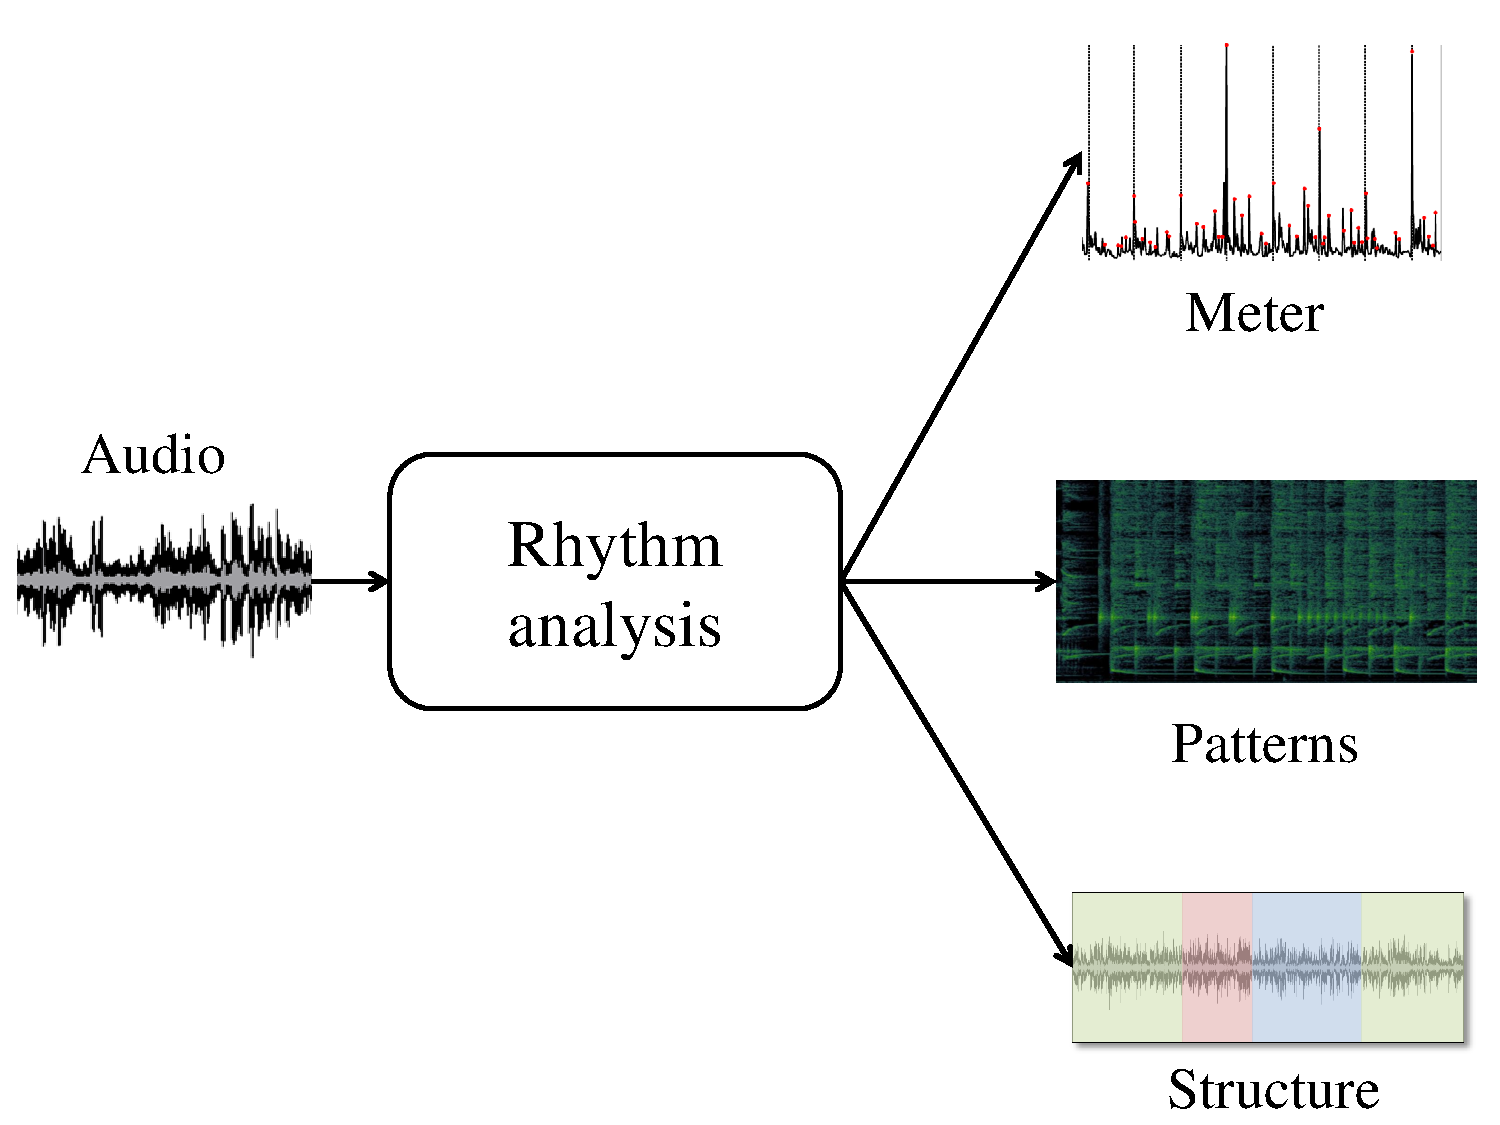
\includegraphics[width=0.9\textwidth]{figs/blockDiags/rhythmAnalysis.pdf}
%\caption[Automatic rhythm analysis from audio]{Example of automatic rhythm analysis from audio recordings estimating meter, rhythmic patterns and structure from audio recordings. The approaches in the dissertation follow a similar flow, with an audio recording being at the centre of analysis.}\label{fig:intro:rhythmanalysis}
%\end{figure}
%
%The thesis aims to bring in as much musical knowledge to the methods as possible, including and using all the known attributes of music. The goal is to build domain specific and informed signal processing and machine learning methods, so that the extracted information is musically relevant and useful. Bayesian models\index{Bayesian model} and methods provide an effective framework to bring in higher level music knowledge into models, in terms of model structure and priors. Bayesian models are hence a central theme for the analysis approaches in the thesis. 
%
%The emphasis of the thesis is on data and methods. The data-driven approaches need good quality datasets, which have been careful compiled and annotated within the context of the thesis. The algorithms are built to work on real world representative music collections - organized curated collections of music that are accessible. 
%
%The thesis focuses only on music analysis and not on music generation, composition and synthesis. The generative models used for analysis in the thesis can however be used for such a task if needed, though it is not the focus of the thesis. In terms of our interaction and experience with music, the thesis focuses mainly on enhanced music listening. Though some of the tools and methods can be useful to both teachers and students of music, it is not the focus of the thesis. 
%
%The work presented is done on well studied art music cultures of India and borrows from the significant musicological literature already available. The thesis however aims to aid musicologists further in their work with these rhythm analysis tools. The data and the methods presented in the thesis can be used by musicologists for large scale corpus level musicological analysis. There are illustrative examples of such analyses in the dissertation, but the thesis does not aim to make any significant musicological conclusions. 
%
%The work in the thesis also borrows from consultation with several musician collaborators over the course of CompMusic project. The analysis methods developed in the thesis do not aim to replace expert musician opinions, but only work within the framework provided by musicians, musicologists, listeners and learners to enhance our experience with music. The problems formulated and addressed in the thesis are on concepts that have well grounded definitions and agreement among the musician and musicologist community. 
%
%In addition to exploring novel approaches to automatic rhythm analysis, the thesis aims to answer the following research questions within the context of rhythm analysis: 
%\begin{enumerate}[leftmargin=*]
% \item It is hypothesized that automatic analysis of rhythmic structures and patterns from audio signals needs specific methodologies that make use of the knowledge about the underlying rhythmic structures. To what extent does incorporating higher level knowledge affect the performance of automatic analysis algorithms? What kinds of higher level information are useful and lead to a better performance? How can such higher level information be included in the framework of Bayesian models to develop novel rhythm analysis algorithms? 
% \item How do the existing rhythm analysis methods designed with different rhythmic structures extend to complex metrical structures in Indian art music? What limitations can we identify of the existing state of the art? 
% \item It is hypothesized that instead of a component-wise disjoint approach to estimating different components of rhythm, it might be useful to jointly estimate all the relevant components together in a single framework. The methods can then utilize the interplay between the components for better estimation. Does a holistic approach work better or is it better to estimate individual components separately? Which components of rhythm are better estimated jointly, and which components can be independently estimated?
% \item It still remains an open question if we need more specialist approaches, or more general approaches that are able to react to a large variety of music. Generally, it appears desirable to have generic approaches that can be adapted to a target music using machine learning methods. What are some such methods, and how can they be useful to adapt it to different music cultures? 
% \item Indian art music and several other music traditions of the world have developed syllabic percussion\index{Syllabic percussion} systems for transmission of their repertoire and technique, which provide a language for percussion in those music cultures. What is the utility of these syllabic percussion systems in automatic percussion pattern analysis? 
% \item Given the availability of useful annotated datasets, one of the questions to ask is if the annotations and the data can be used for a corpus level analysis leading to meaningful and valid musicological conclusions. 
%\end{enumerate}
%
%Broadly, the thesis identifies the challenges and opportunities in automatic rhythm analysis of Indian art music, formulates several rhythm analysis tasks, addresses the issues with building datasets for rhythm analysis, and then focuses on the tasks of meter and percussion pattern analysis. 
%
%The scope of the thesis within CompMusic is to provide rhythm analysis tools and methods to be a part of the comprehensive set of content based analysis methods for the music cultures under study, with the final goal of utilizing these analysis methods to define musically relevant similarity measures. 
%
%A major strategy of CompMusic is open and reproducible research - to be open in sharing ideas, goals, results, data and code as widely as possible. All the data, code and results presented in the thesis will be available openly or be accessible to the research community. Whenever possible, resources will be provided to reproduce the results of the thesis. The data and code will be shared with the community through open source platforms under open licenses. An open dissemination strategy is one of the primary objectives of the thesis. 
%% \comment{Write about the broad tasks addressed in the thesis, so that Chapter 2 (background) has a better context.}
%\section{Organization and thesis outline}
%The dissertation has seven chapters. Each chapter is written on a major topic of the thesis and is aimed to be self contained with a short introduction, content, and a summary. The writing style followed in the thesis is a mixture of both active and passive voice. Most of the dissertation derives content from published research papers describing the work done by collaborative teams. Hence the word `we' refers to the author and when applicable, additionally includes the co-authors and collaborators in research papers. When presenting results and making observations, the word `we' further includes the reader who can equally make such an observation from the results. However, the main original contributions by the author of the thesis are emphasized appropriately, wherever needed. 
%
%After an introduction to the thesis in \chapref{chap:intro}, \chapref{chap:bkgnd} provides an overview of the music background and a review of the state of the art as needed for the thesis. \chapref{chap:probdef} is focused on identifying and discussing several novel automatic rhythm analysis problems in Indian art music. \chapref{chap:datasets} presents the research corpora and all the rhythm related datasets compiled as a part of CompMusic project that will be used for various rhythm analysis tasks. \chapref{chap:meterInfTrack} and \chapref{chap:percpatt} are the main chapters of the dissertation discussing the topics of meter analysis and percussion pattern discovery, respectively. \chapref{chap:conclusions} presents some of the applications and conclusions with pointers for future work. In addition, the links to resources from the thesis (data, code, examples) are listed in \appref{app:resources}. There are several new non-standard terms in the dissertation including unfamiliar terms related to Indian art music which are all listed with a short description in a glossary in \appref{app:glossary}. The glossary also lists the acronyms used for datasets and analysis methods in the dissertation. 
%
%\chapref{chap:bkgnd} provides an overview of the background material necessary for the thesis. It introduces a concrete terminology for rhythm concepts and a basic introduction to rhythm and percussion in Indian art music and Beijing opera. It then provides an overview of the state of the art for automatic rhythm analysis in \gls{MIR}. The chapter ends with a brief overview of the technical concepts useful to understand the thesis work better. The content of the chapter is compiled and presented from several external sources cited appropriately when necessary. 
%
%\chapref{chap:probdef} identifies several challenges and opportunities to automatic rhythm analysis in Indian art music. The chapter aims to present all identified relevant research problems, while only a subset of them are addressed in the thesis. For these problems, the chapter also presents an overview of the state of the art when available. It further elaborates and formulates the thesis problems that are addressed in detail in the next chapters of the dissertation and presents an evaluation of the state of the art for some of these tasks on Indian art music. A large part of the content of the chapter is derived from several discussions of with collaborators of CompMusic, musicians, musicologists and listeners on what they consider are important rhythm analysis problems, with some content and results from our published journal article \cite{ajay:14:rhythmJNMR}. 
%
%\chapref{chap:datasets} describes the efforts of CompMusic in compiling and annotating the research corpora and test datasets. The chapter presents a systematic framework to elucidate a set of design principles to build data corpora for research in Indian art music \cite{serra:14:corpus}. All the annotated rhythm related datasets are described in detail emphasizing on the research problems in which they are useful. Other state of the art datasets that are used in the thesis are also described. Apart from being useful as test datasets to evaluate algorithms and approaches, annotated datasets are also useful to infer musically meaningful observations. Hence an illustrative corpus level statistical analysis of relevant test datasets is also presented to point out some interesting observations. The rhythm related datasets described in the chapter have a major contribution from the author, but still are collective efforts of the CompMusic team, as indicated with each dataset. Some of the content of the chapter is from our published papers~\cite{ajay:14:smc,ajay:14:talaTrack,tian:14:icassp,ajay:14:ismirbo,gupta:15:tabla,ajay:16:spmodel} while some of it is unpublished content. 
%\begin{figure}
%\centering
%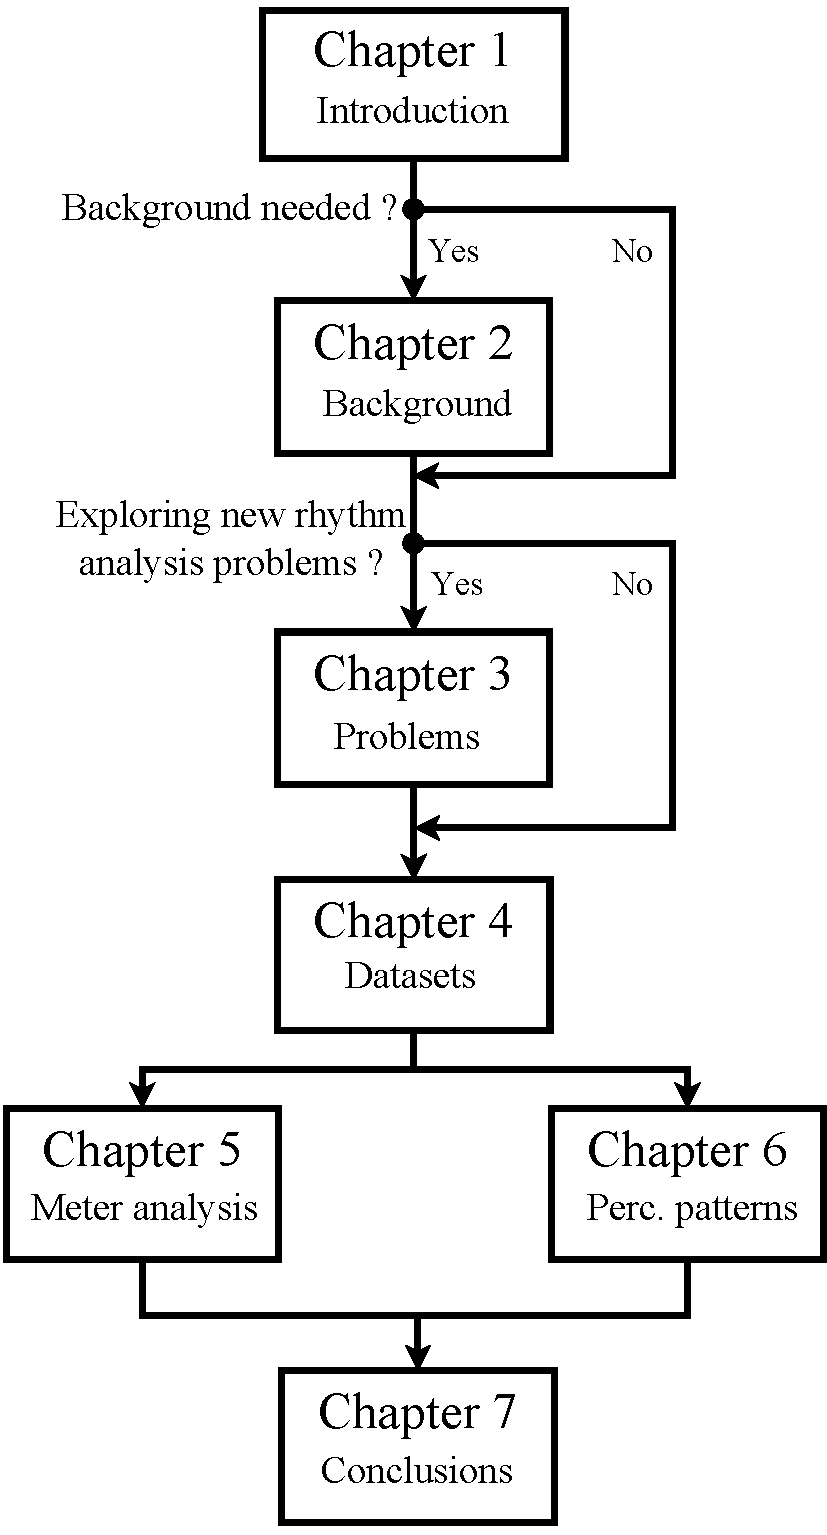
\includegraphics[scale=0.52]{figs/blockDiags/chapterOrg.pdf}
%\caption[Dependencies between the chapters of the dissertation]{Dependencies between the chapters of the dissertation, also indicating a suggested reading order for the chapters}\label{fig:intro:chapread}
%\end{figure}
%
%\chapref{chap:meterInfTrack} presents the primary contribution of the thesis and describes one of the main research problems addressed. The chapter focuses on the problem of meter analysis and describes several approaches to the task in the context of both Carnatic and Hindustani music of India. The chapter proposes novel Bayesian models and novel inference algorithms for different levels of informed meter analysis, with a comprehensive evaluation on annotated datasets. The content of the chapter is derived from the current state of the art in beat and downbeat tracking~\cite{krebs:13:bpm,krebs:15:pf}, along with some of our recently published papers~\cite{ajay:14:talaTrack,ajay:15:pf,ajay:16:spmodel,holzapfel:14:odd} and from latest unpublished work. 
%
%\chapref{chap:percpatt} presents the other important contribution of the thesis and describes the task of percussion pattern discovery in Indian art music. The work presented in the chapter is preliminary and exploratory, but demonstrates the effective use of syllabic percussion systems in representation, transcription and search of percussion patterns in percussion solo recordings. As a preliminary test case, experiments on percussion pattern classification in Beijing opera are presented. The approaches are extended to Indian art music and an evaluation is provided on drum solo datasets. A part of the results presented in the chapter are derived from our published papers \cite{gupta:15:tabla,ajay:14:ismirbo} while many results are yet unpublished. \chapref{chap:conclusions} presents some of the applications and conclusions. The chapter summarizes the results from different chapters and presents pointers for future work. 
%
%Each chapter of the dissertation is self contained and can be read in isolation with sufficient background. However, the following dependencies exist between chapters, which is a possible indicator of the recommended order for reading and is further summarized in \figref{fig:intro:chapread}. Starting with \chapref{chap:intro}, if the reader has sufficient background on rhythm in Indian music and rhythm analysis problems in \gls{MIR}, \chapref{chap:bkgnd} would be a recap. For a researcher starting out and exploring new problems and resources in Indian art music, \chapref{chap:probdef} and \chapref{chap:datasets} might be more interesting. \chapref{chap:meterInfTrack} and \chapref{chap:percpatt} focus on separate research problems and can be read independently. \chapref{chap:datasets} might be necessary to understand the evaluations presented in \chapref{chap:meterInfTrack} and \chapref{chap:percpatt}. \chapref{chap:conclusions} might be useful to understand some of the applications in more detail. \appref{app:resources} and \appref{app:glossary} can be used as quick guides for resources and term definitions, respectively. 
%
%To the best of our knowledge, this dissertation is the first comprehensive attempt at rhythm analysis of Indian art music. By addressing the problems discussed in this dissertation within the context of CompMusic project, we aim to develop useful tools and algorithms for automatic rhythm analysis of Indian art music. Integrated into Dunya, we hope that these tools will provide an enriched experience to a music listener, enhanced through a cultural context. In the process, we also hope to obtain a better understanding and provide deeper insights into the nature of rhythm in Indian art music, and contribute to improving the state of the art in \gls{MIR}. 

\noindent We live in a world with explodingly increasing data and information. The information and communication technologies (ICT) help us assimilate, organize, interpret, interact, consume and generate these data and information, enhancing the experience with knowledge of the world. The technologies are kept developing to follow the fast-evolving sociocultural context, in which we build tools and devise new methods.

Music is a necessary part of many people's lives. Teaching and learning music is not only a hobby but a professional commitment of many people. The knowledge-learning experience has been updating rapidly in the past few years along with the fast developing ICTs. A large amount of amateur or professional learners are converted into the online education environment, thus benefited from its easy-accessibility, various course content, and most importantly, the automatic practice assessment feedback which is used to keep the learners aware their shortcomings and gets their skill improved. Music performance, as a type of knowledge and skill, although different and more abstract than other subjects. Its online learning requires automatic tools to adapt to such context and widely diverse learners.

Music Information Retrieval (MIR) is a specialized field within the music technology, in which people invent and develop methods and tools to analyze, synthesize, understand and represent the music. It aims to explain the music concepts at various levels and build computational models for the human music perception and understanding aspects, such as melody, rhythm, timbre, harmony, structure, mood. Automatic music performance assessment in MIR aims to extract perceptual and semantic representations in music performance recordings and devise computational models for the performance assessment.

Music has many elements. The singing voice is one of those elements which plays the central role in songs, and it's the main attraction for listeners. The pronunciation aspect of the singing voice is essential in many music traditions as it conveys the semantic information of the lyrics and the aesthetic pleasure to the listeners. This work takes the MIR point of view dealing with automatic singing voice assessment and focusing on the pronunciation aspect: to segment pronunciation meaningful singing voice events, extract pronunciation meaningful representations and develop computational models to assess the pronunciation correctness and measure the pronunciation similarity.

The work presented in this dissertation lies in the automatic music performance assessment subject of the MIR field, aiming at domain-specific analysis and assessment approach within a culture-specific context. We now reach the context and motivation of the thesis. The scope and objectives are then defined. Finally, we describe the organization and thesis outline. 

\section{Context and relevance}

In the last two decades, many new methods, models and algorithms have been developed in the MIR community, which significantly promoted the advancement of the fields of sound and music computing, and music technology. Initially, the MIR research has been restrained to eurogeneric music. Not until recently, we witness an increasing amount of researchers who devote themselves to the MIR research of non-eurogeneric music. The CompMusic project plays an essential role in boosting this trend.

CompMusic (Computational Models for the Discovery of the World's Music) is focused on the advancement in the field of MIR by approaching new challenges from a culture-specific perspective. CompMusic aims to develop computational models for several non-western music traditions and in the meantime, advance the overall development of MIR. CompMusic studies five music traditions: Jingju (also known as Beijing opera, China), Hindustani (North India), Carnatic (South India), Turkish-makam (Turkey), and Arab-Andalusian (Maghreb).  The current information technologies in MIR field are typically targeting to solve the problems emerging from the western music. However, a wide range of music traditions other than western music can bring many new challenges. The motivation behind CompMusic is to face these new challenges by studying the five non-western music traditions, and to develop MIR technologies to embrace the richness of the world's music.

CompMusic further aims to understand music both perceptually and semantically. The typically MIR methods revolve around the audio-centric idea, which parses the incoming audio into high-level music events or concepts, such as onsets, notes, beats, melodies and chords. Although all music traditions share some common concepts, each one has its unique perceptual or semantic attributes that require different interpretations. Additionally, music is encapsulated in a complex sociocultural and historical context, which affects deeply the way of how we interpret it. Many attributes of the five non-western music traditions studied in CompMusic project cannot be explained by the audio or the western music knowledge themselves. Thus, a deeper understanding can only be achieved by considering additional culture-specific information.

Delving into the problems brought by diverse music traditions will not only help develop technologies for the specific tradition, but also will extend the scope of the existing MIR technologies, making them more adaptable and robust, and eventually open a new path in the MIR research field. Delving into these problems can also break off the limitation of current MIR technologies by posing new issues. 

CompMusic focuses on the extraction of the features from music audio recordings related to melody, rhythm, timbre, pronunciation and on the perceptual and semantical analysis of the contextual information of these recordings. The goal is to identify and describe the culture-specific music perspective and to develop perceptual and semantical meaningful computational models with them. The research in CompMusic is data-driven, hence it builds upon research corpora. The types of data collected for the corpora of each music tradition are mainly audio recordings, then accompanied with metadata, scores, lyrics, etc. To construct the research corpora is one of the main goals of CompMusic project.

The work presented in this dissertation has been conducted in the context of the CompMusic project, focusing on automatic singing voice pronunciation assessment for jingju music from a data-driven perspective using signal processing and machine learning methodologies. This dissertation assimilates the aimings and context of the CompMusic project as applied to automatic singing voice analysis and assessment.  By facing the challenge and building the culture and domain-specific singing voice analysis and assessment models, we also acquire a better understanding the existing MIR tools, and would eventually improve their capabilities. The development of the newer algorithms, models and technologies allow enriching the current knowledge of world's music and provide a novel sociocultural and musical perceptual insight. Such a work in this dissertation is relevant since we push the boundaries of automatic singing voice assessment to address the new challenges of different music traditions in the world. 

\section{Motivation}
Singing is the simplest form of music-performing and making since it doesn't require any external musical instrument. The important role of the singing played in the music education and performing cannot be over-emphasized. Since everyone can practice singing without an instrument, all the music aspects - melody, rhythm, timbre, dynamic, pronunciation, expression and so on can be studied by singing and also internalized by singers.

Singing is an act of producing musical sounds by voice using augmented speech tonality, rhythm, pronunciation and various techniques. The music of singing contains events and structures organized in time, in other words, it's an event-based occurrence. Thus segmenting the musical events is an important task in conducting singing analysis and assessment. The automatic segmentation, analysis and modeling of these singing events can help us to elaborate perceptual and semantical meaningful measures for the singing voice assessment.

Musical events are often organized in a hierarchical way which further forming the musical structure.  Estimating event onsets and boundaries related with the singing is dispensable for the further analysis and assessment from a microscopic perspective. All the melodic, rhythmic or lyrical phrases in singing voice are established upon the basic musical or articulative event, such as the musical notes, singing phonemes, syllables and words. Each of the events can be estimated in an isolated way. However, due to the hierarchical structuring of them, a hierarchical estimation approach needs to be exploited as an important MIR task.

Singing voice can be perceptually appreciated from several musical or articulative dimensions (pitch, rhythm, timbre, dynamic, expression, pronunciation). Some of them are musically well-defined and can be assessed by relatively objective measures, such as melody, rhythm, dynamic. Others are more abstract and subjective due to the natural character of these dimensions. To sing in an accurate pitch and rhythm, have a pleasurable dynamic variation and be expressive are some high-quality singing traits commonly shared with many music traditions. However, due to the specificity of the Chinese tonal language and the strict obligation during the oral transmission, jingju singing education is extremely demanded in reproducing accurately the teacher's singing pronunciation at syllable and even phoneme level.

Tools developed for automatic singing voice assessment can be useful in a large number of applications such as computer-aided singing teaching, enhanced navigation of music collections and content-based music retrieval. The target users of these tools extend across professional singers who pursue to convey perfect singing details, amateur singing students who seek to have a professional assessment feedback to improve their singing abilities, musicologies who can use these tools for visualizing some singing perceptual concepts and music streaming services who can use these tools to align the lyrics to the audio.

Due to the artistic nature of the music, music performance teaching should be done individually regarding the different skill level of the students, hence it's a time-consuming and resource-intensive work. A music teacher is only able to tutor a limited number of students in a class. However, with large and ever-growing students participating in online music performance courses, the limited teacher human power cannot meet the requirement of such large amount of audience. Thus, automatic assessment and feedback need to be provided to achieve an effective learning experience in a scalable way. 

The automatic assessment of singing voice can be conducted on different singing events granularities (entire song, melodic phrases, lyrical lines, onsets, syllables, phonemes) and on various dimensions (pitch, rhythm, dynamic, timbre, pronunciation, expression). Further, the assessment can be template-based, where the student's singing is compared by measuring the similarity with a reference singing; or non-template-base, where the student's singing is assessed by a predefined model. In the template-based case, there is a need to develop perceptual relevant and content-based similarity measure; and in the non-template-based case, it necessitates to define the assessment model.

As specified earlier, a meaningful singing voice assessment model can be better achieved by taking into account the context of the music tradition - incorporating high-level musical knowledge into the assessment of the singing voice on the culturally meaningful event granularities and musical dimensions. This requires identifying unique challenges for the current MIR technologies and combining information from both raw data sources and high-level musical knowledge to build computational models.

With a unique spoken language system and a strict convention of oral transmission, jingju music singing poses a big challenge to the state of the art in automatic singing voice assessment. Several automatic singing voice assessment tasks in jingju music singing have not or very few studied before. With such unique characteristics, studying the automatic singing voice assessment for jingju music can help to pinpoint the limitations of current approaches, improve their performance, and eventually open up new paths for further research on this topic. As mentioned earlier, the gap between the current state of the art capacities of MIR technologies and the need of the multicultural world is huge. This applies as well to jingju music, in which the current methods come short of using its culture-specific knowledge and restrict the assessment performance. Being well-established music tradition in China and with a large amount of audience around the world, jingju music is an ideal candidate to develop novel automatic singing voice assessment methods.

\section{Score and objectives}

The work presented in this dissertation on automatic singing voice assessment comes to the crossroad of audio signal processing, machine learning, musicology and the application of online music education. Automatic singing voice assessment can be a very broad topic and may extend to many detailed sub-topics. Thus, it is necessary to define the scope of the research in this dissertation and elucidate the research questions and objectives. The objectives of this research are listed below:

\begin{itemize}[leftmargin=*]
\item To identify challenges and opportunities in automatic singing voice assessment of jingju music and formulate pertinent automatic singing voice assessment problems. Convert musical definitions and concepts into engineering formulations compliant with computational modelling using signal processing and machine learning approaches.
\item To build annotated jingju singing voice audio and symbolic collections focusing on automatic pronunciation assessment for the computational model training and testing.
\item To construct culture-aware computational models for automatic jingju singing voice analysis and assessment.
\item To develop novel machine learning models for the music event segmentation, pronunciation representation and assessment of jingju singing voice.
\item To explore the extensions of the specific computational models to western music culture with the application of automatic solfège assessment. 
\end{itemize}

The final goal of this dissertation is to devise culture-specific representations for jingju singing voice events, and to use these representations for the automatic assessment modelling. The focus of the research is on jingju music singing voice, while we also explore extensions to western solfège assessment problem.

\begin{figure}
\centering
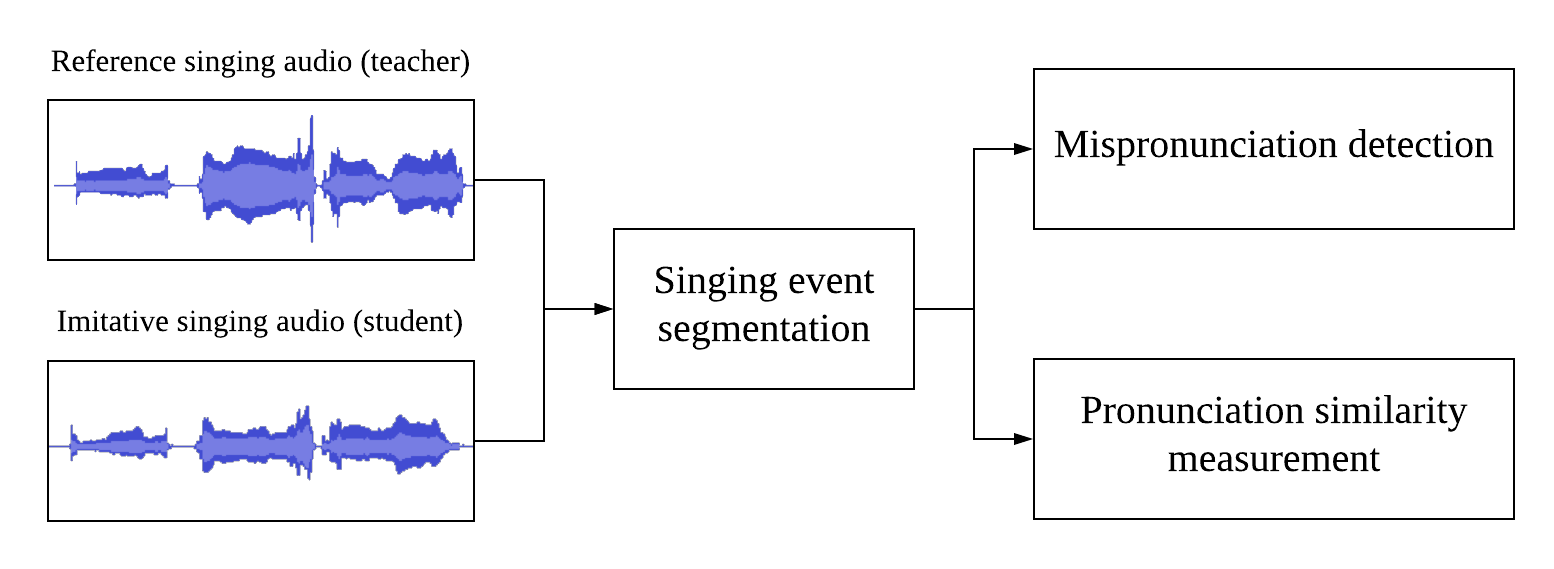
\includegraphics[scale=0.2]{figs/blockDiags_rong/ch1_motivation_audio.png}
\caption[Example of automatic singing voice assessment from the reference and imitative singing audio recordings]{Example of automatic singing voice assessment from the reference and imitative singing audio recordings, estimating singing event segments, assessing the special pronunciation correctness and measuring the pronunciation similarity. The methods in this dissertation follows the similar diagram, with the audio recordings as the major information source.}\label{fig:intro:chapread}
\end{figure}

This dissertation investigates data-driven signal processing and machine learning approaches for automatic assessment of singing voice audio recordings. An audio recording is thus the primary source of information on which the computation models are built. \figref{fig:intro:chapread} shows an example of such diagram, presenting three assessment tasks - singing event segmentation, special pronunciation correctness assessment and pronunciation similarity measurement all adopt the audio recordings as the major information source. Other musical data sources such as musical scores, lyrics and editorial metadata are secondary, however, used in some tasks. The approaches adopted in this dissertation are mainly audio signal processing and machine learning (deep learning and probabilistic graphical models), investigating supervised learning methods to develop automatic singing voice assessment models.

This dissertation works toward to bring knowledge related to jingju music teaching and jingju music language to the methods. We aim to build knowledge-informed machine learning methods so that the extracted representations of the musical events and computational models are culturally relevant. High-level knowledge is taken as the determinants in the task and computational model designing.

The data-driven methods adopted in this dissertation require good quality and real-world data collections. We carefully collected, annotated and compiled the research datasets in align with the goal of building assessment models. The algorithms are developed to perform on the real world music teaching scenarios - on the singing audio recordings of the actual classroom teaching.

The investigation in this dissertation is focused on developing novel automatic singing voice assessment methods and technologies, which are based on well-studied musicological knowledge of jingju music culture. Although the data and methods presented can eventually be adopted by musicologists for large-scale corpus analysis, the work does not aim to make any musicological contributions.

The musicological and music teaching knowledge adopted in this work is borrowed partly from the consultation with jingju performing teachers, students and jingju musicologists. The assessment models developed in this dissertation are by no means a replacement of expert music teachers, but only serve within the support of music teachers, musicologists, and as a guidance to jingju singing learners. In addition to developing novel approaches for automatic singing voice assessment, this dissertation aims to answer the following research questions:

\begin{enumerate}[leftmargin=*]
\item How do existing automatic music performance assessment methods developed within different musical context extend to jingju music? What limitations can we pinpoint from the current state of the art?
\item We assume the high-level musicological and music teaching knowledge is useful for defining research problems, tasks and helping design computational models. What kind of high-level knowledge are insightful? How and to what extent can such knowledge be used to achieve the goal?
\item It is hypothesized that music performance assessment is conducted on various musical or articulative event granularities and different musical dimensions. Which event granularities and which musical dimensions can bring new and unique challenges to this research topic, and in return, to generalise the existing state of the art methods?
\item What are machine learning methods or deep learning architectures which are able to learn the musical dimension-relevant representations on the variable-length musical events? What kind of side information is useful for the singing voice event segmentation and assessment? How can these side information be included in the machine learning framework?
\item It is assumed that the methods devised in this work are culture-specific. Generally, it is desirable to have a generalised method that can be transferred to other music cultures. How can the methods proposed in this work be adapted to a different music culture? 
\end{enumerate}

In general, this dissertation identifies the challenges and opportunities in automatic singing voice assessment of jingju music, formulates several assessment problems and tasks, tackles the issues with constructing datasets, and finally focus on the tasks of singing events segmentation, special pronunciation correctness assessment and pronunciation, overall quality similarity measurement. The scope of this dissertation within CompMusic is to support singing voice assessment methods and tools to be a part of the inclusive set of content-based analysis approaches.

One of the main advocacies of the CompMusic project is open and reproducible research - openly sharing ideas, objectives, data, code and experimental results. All the data, code and experimental results presented in this dissertation will be openly accessible via open source platform (Github, Zenodo) under open and non-commercial licenses.

\section{Organization and thesis outline}

The dissertation has eight chapters. Each chapter is written on a main topic of the thesis and is aimed to be self-contained unit with introduction, main content and summary. After an introduction of the dissertation in Chapter 1, Chapter 2 presents an overview of the jingju music background and a  state of the art review of the related research topics. Chapter 3 is engaged in elucidating several new automatic singing voice assessment problems in jingju music. Chapter 4 discusses the jingju music research corpora and mainly the a cappella singing voice datasets that will be used for several singing voice assessment tasks. Chapter 5, 6 and 7 are the major chapters of this dissertation presenting the works of automatic singing syllable and phoneme segmentation, syllable-level special pronunciation assessment and phoneme-level pronunciation similarity measurement. Chapter 8 presents applications, conclusions and future works. The links of external resources such as data, code are listed in Appendix B. Jingju music-related terms and technical acronyms used in the dissertation are listed as a glossary in Appendix C. 

%TODO: for each chapter, use one paragraph to describe the outline 


\chapter{Background}\label{chap:bkgnd}

\section{Jingju music}
Jingju (also known as Beijing or Peking opera) is the most representative form of Chinese opera which assimilates the essence of various Chinese opera forms such as 徽剧 (Anhui opera), 昆曲 (Kun opera), 秦腔 (Qin qiang) and 高腔 (Gao qiang). It arose in the late 18th century and became fully developed in the mid-19th century. Now it is regarded one of the cultural treasures in China and inscribed in the UNESCO representative list of the intangible cultural heritage of humanity. Jingju is widely practised over mainland China, Hong Kong, Taiwan, and overseas countries where there is Chinese communities presence. Major jingju performing troupes are located in big mainland China cities such as Beijing, Tianjin and Shanghai. A significant amount of jingju musicological literature can be used to formulate MIR problems. The presence of a large audience and musicological literature are an important motivation to carry a computational research for this music culture.

This section describes the focus of this dissertation -- jingju music culture. The emphasis is on singing concepts in this music culture. This section is not a comprehensive introduction to this culture but is aimed to be sufficient to support the following chapters of the dissertation.

We use simplified Chinese characters (computer encoding: GB2312) to introduce jingju terminologies for the first time in this dissertation. We also introduce the pinyin, the romanization system of Mandarin Chinese, for each terminology. Only the pinyin form of the terminology will be used throughout the dissertation. 

\subsection{A synthetic art form}

Professor Li in National Academy of Chinese Theatre Arts (NACTA) said ``The three basic elements of Chinese opera are 曲 (pinyin: qu, tune), 程式 (pinyin: chengshi, conventions -- a strict set of rules) and 虚拟表演 (pinyin: xu ni biao yan, virtual acting). These three elements are ultimately aiming to support 戏 (pinyin: xi), which can be approximately understood as `entertainment'." Of the three elements, ``tune" is the most important one, which represents all the musical dimensions of the jingju music. However, this representation is not only limited to music but constructs the whole skeleton of the jingju performing.

Jingju is a synthetic art form which includes four disciplines -- 唱 (pinyin: chang, singing),念 (pinyin: nian, declamation),做 (pinyin: zuo, physical acting) and 打 (pinyin: da, acrobatics). Singing is directly related to tune, and the other three disciplines are integrated together by the music and rhythm of jingju performing. 

The jingju technical training for performers consists in becoming proficient of the conventions of the four disciplines as mentioned earlier which are established by tradition. The jingju performers use these conventions to construct characters and convey stories. For example, they use singing conventions to express the character's emotional state. The jingju performance is codified through the conventions which are not aimed at hinder the creativity and artistry. The appreciation of the beauty of jingju is to see how the performers are conveying the conventions. In jingju training, a performer will have more creativity if she/he can master more conventions.

\subsection{Singing and instrumental accompaniment}

``In the aural performance of Beijing opera, two types of sounds are actually heard: song and speech vocalized by the stage performers, and instrumental music played by the musicians of the orchestra. The voice of the Beijing opera performer, is the featured component of aural performance." -- Elizabeth Wichmann.

In a jingju play, the sections where singing occurs are 唱段 (pinyin: chang duan, literally translated as singing section). The closest form to chang duan in Western opera is "aria", which signifies "any closed lyrical piece for solo voice (exceptionally for more than one voice) with or without instrumental accompaniment, either independent or forming part of an opera, oratorio, cantata or other large work." The difference between chang duan and aria is that latter is a self-sufficient piece conceptually, whereas chang duan is formulated in a dramatic continuum, although it is usually performed and recorded individually [ref Rafa thesis]. 

Jingju chang duan is started actually before the performer starts to sing. The declaration of the starting point of a chang duan is 叫板 (pinyin: jiaoban, literally translated as "calling the banshi"). Banshi is the rhythmic framework concept that we will introduce it in \secref{sec:banshi}. Jiaoban is included in every chang duan of the commercial recordings and teached in conservatory jingju performing classes. The percussion pattern 住头 (pinyin: zhu tou) is to signal the end of a chang duan.

Jingju instrumental ensemble is divided into two sections -- 文场 (pinyin: wenchang, literally translated as "civil scene") and 武场 (pinyin: wuchang, literally translated as "martial scene"). Wenchang is the orchestral accompaniment, and wuchang is formed by percussion instruments. There are five basic percussion instruments -- 单皮鼓 (pinyin: danpigu, drum), 板 (pinyin: ban, clappers), 铙钹 (pinyin: naobo, cymbals), 大锣 (pinyin: daluo, big gong), 小锣 (pinyin: xiaoluo, small gong). The first two instruments are played normal by the same person, so they have a combined term -- bangu. The musician who plays the bangu is called 司鼓 (pinyin: si gu), literally translated as "the man who is in charge of the bangu". The primary functions of wuchang are playing 锣鼓经 (pinyin: luo gu jing, rhythm patterns) and supporting the rhythmic aspect of the actor/actress’ performing.

The main instrument of wenchang is 京胡 (pinyin: jinghu). Having loud volume, and very bright and penetrating sound, jinghu is the aural representative of jingju sound. The musician who plays jinghu is called 琴师 (pinyin: qin shi, master instrumentalist). The major role played by qinshi is supporting the jingju melody. Traditionally, qinshi is the musician who has the closest collaboration with the performer. Jingju line sustains the singing line to form an uninterrupted melody stream, which impels the singing. 

The other instruments in wenchang are 月琴 (pinyin: yueqin), 三弦 (pinyin: sanxian), 京二胡 (pinyin: jingerhu), 阮 (pinyin: ruan), 中阮 (pinyin: zhongruan) and 大阮 (pinyin: daruan). They all play the same melody as the jinghu line in the same or different octave, and in a heterophonic structure. The performer, sigu and qinshi take turns in coordinating the jingju performing tempo.

\subsection{Lyrics structure}

The primary function of the lyrics in jingju is telling stories. Music structure in jingju is closely related to lyrics structure. The tune sequences in jingju are inherited from the creation principle in poetry of Tang dynasty (618 - 907 AC), that the melody and poetic structure are taken from the preexisting poems or songs, and new lyrics are arranged to fit in that schema. The new lyrics are labelled with the name of the original poem or song, so that the performer knows how to sing the tune. The label of the original poem or song is called 曲牌 (pinyin: qu pai, literally translated as tune label). Different qupai have different forms which represent not only different melodies but also a different number of melodic lines and a different number of characters in each line. This kind of lyrics structure is called 长短句 (pinyin: chang duan ju, literally translated as long and short lines). A jingju chang duan consists of a sequence of these chang duan ju.

The basic structure of lyrics stanza consists of two symmetrical lines which have the same number of characters. The most common term in jingju circles for describing this two symmetrical lines is 上下句 (pinyin: shang xia ju, literally translated as upper and lower lines). The most common English terminology for shang xia ju is couplet for the stanze, opening line for upper line and closing line for lower line. A standard line has either 7 or 10 characters, grouped in three sections -- 2 + 2 + 3 or 3 + 3 + 4. These sections, namely 逗 (pinyin: dou), are the basic semantic and rhythmic units.

The lyrics structure mentioned above can be modified in actual singing. A typical case is the variation of the number of characters in each line, for example, 衬字 (pinyin: chenzi), the characters do not have semantic meaning, but serve to help the performer prolong the singing of certain nasal or vowel sounds. Another form of increasing the number of characters is 垛字 (pinyin: duozi), which inserts semantic units containing 3 or 4 characters into the line.

\subsection{Linguistic tones and pronunciation}

It is commonly assumed that the linguistic intonation of a tonal language singing needs to agree with its melody to a certain extent to make sure the intelligibility. For jingju which is sung by using mainly Chinese Mandarin language and various dialects, its music features are related to the dialects. In other words, The Chinese dialects used in jingju singing determines its melody characteristics to a certain extent.

In jingju circles, it exists an expression to describe the relation between linguistic tones and melody -- 字正腔圆 (pinyin: zi zheng qiang yuan, literally translated as “characters should be straight, tune should be round.”). This expression can be understood as that the performer needs to attain both the intelligibility of the lyrics and the smooth sounding of the melody. The most critical problem to be avoided in jingju singing is 倒字 (pinyin: dao zi, literally translated as upside-down character), which means that the lyrics is misunderstood because the performer mispronounces certain characters.

Most of the jingju scholars agree in that jingju singing uses mainly two Chinese dialects -- 北京音 (pinyin: Beijing yin, the dialect of Beijing) and 湖广音 (pinyin: Huguang yin, the dialect of Huguang). Some scholars consider that jingju singing also uses a third Chinese dialect -- 中州韵 (pinyin: Zhongzhou yun, literally translated as rhymes from Zhongzhou). All three dialects share the same tone categories 阴平 (yin ping), 阳平 (yang ping), 上 (shang) and 去 (qu), although the pitch contours of the same characters realized in the same categories are different for the three dialects.

The three dialects result in the complexity of the pronunciation in jingju singing. Such complexity influences the linguistic tones as well as the pronunciation of the syllabic initials and finals. The standard Chinese used in Mainland China -- 普通话 (pinyin: pu tong hua), very close to Beijing yin, is taken as the reference for jingju pronunciation. All the special pronunciations different from the reference putonghua can be divided into two categories -- 尖团字 (pinyin: jian tuan zi, literally translated as pointed and rounded characters) and 上口字 (pinyin: shang kou zi, literally "up to the mouth" characters). Jian tuan zi has two sub-categories of characters -- 尖字 (pinyin: jianzi) and 团字 (pinyin: tuanzi), which are separated by the fricative and affricative consonants of a syllable. When studying a new play, jingju performer should learn which characters belonging to tuanzi in putonghua should be pronounced as jianzi. The jian tuan zi qualities are considered extremely important for both listening comprehension and aesthetic effect. Shang kou zi are generally a set of characters of which the pronunciation is different from the standard Mandarin, adopting from southern Chinese dialects -- Huguang yin and Zhongzhou yun. By shang kou zi and converting certain tuanzi to jianzi, the language of jingju is made more appealing to speakers of the diverse range of dialects throughout China than is Mandarin alone. Jian tuan zi and shang kou zi are one of the main study focuses of this dissertation. Thus a more specific extended description will be presented in section. 

\subsection{Role-types}

行当 (pinyin: hang dang), commonly translated as role-type, is a colloquial term for the “acting profiles” of a jingju performing character. There are four role-types in jingju -- 生 (sheng), 旦 (dan), 净 (jing) and 丑 (chou), which respectively have their specific styles of performing, speaking, singing, costume, and make-up. These oral and visual means of expression define the gender, approximate age, social status, profession, personality and singing style. Due to the various and complicate conventions that each role-type possesses, every performer has to specialize one role-type and practice these conventions along the performing career. 

\begin{table}[ht!]
\centering
\begin{tabular}{l|cccc}
\toprule
Main role-types & sheng               & dan                           & jing & chou \\
\midrule
\multirow{4}{*}{Sub role-types} & laosheng\textsuperscript{*} & qingyi\textsuperscript{*} & tongchui    & wenchou   \\
& xiaosheng & huadan & jiazi & wuchou \\
&&laodan&& \\
&&wudan&& \\
\bottomrule
\end{tabular}
\caption{Jingju four role-types and their sub role-types. The role-types with * superscript are the main research objects of this dissertation because singing is their major discipline.}
\label{tab:role-types}
\end{table}

Sheng role-type is specialized in the performance of male characters, whereas dan role-type is specialized in that of female characters. Jing role-type depicts the male characters with an exaggerated temperament. Chou role-type is used for male or female comic characters. The most obvious difference between the male’s voice and the female’s voice is the timbre. Male role-types sing with chest voice, while female role-types use falsetto. Regarding the singing pitch register, there is a displacement of the pitch range in the female singing to a higher region, where female sings a fourth to an octave higher than male singing. Regarding melodic contours, female singing is usually more melismatic than male singing. 

老生 (pinyin: lao sheng) role-type portrays adult or old male characters, which is also the representative of male singing. All textbooks use the examples of laosheng role-type to explain elements of jingju music system. Two representative sub-role-types in dan are 青衣 (pinyin: qing yi) and 花旦 (pinyin: hua dan). The former is most representative role-type of female singing, and generally used for building female characters from a higher social classes. The latter is used for building female characters with a playful personality.

We list the major jingju role-types in \tabref{tab:role-types}, where laosheng and qingyi are the main research objects of this dissertation since singing is their major discipline.

\subsection{Shengqiang}

There is no a coherent definition of jingju 声腔 (pinyin: shengqiang) between scholars. Some of them define shengqiang as tune families of jingju music, meaning a tune which has been evolved into different versions in the performing and transmission process throughout the history. Although these tunes share certain tonal, modal, and dramatic function, they tend to differ from each other in metrical, rhythmic, and melodic details. The shengqiang definition of Elizabeth Wichmann deviated from tune family, and characterize a group of related shengqiang as system. Each shengqiang system is identified by its unique patterns of modal rhythm, song structure, melodic contour and construction, and keys and cadences.  

Jingju contains mainly eight shengqiang -- 西皮 (xipi), 二黄 (erhuang), 反西皮 (fanxipi), 反二黄 (fanerhuang), 四平调 (sipingdiao), 南梆子 (nanbangzi), 高拨子 (gaobozi) and 吹腔 (chuiqiang). Two shengqiang with the most significant presence in jingju arias are xipi and erhuang. Fanxipi and fanerhuang are respectively first degree shifted versions of xipi and erhuang. Additionally, shengqiang is related to the emotional content of the aria. For example, Wichmann describes the emotional content of erhuang as dark, deep, profound, heavy and meticulous, and xipi as sprightly, bright, clear, energetic, forceful, purposeful. 

\subsection{Banshi}\label{sec:banshi}

Ban means the percussion instrument clappers used in jingju wuchang. Banshi can be understood as the jingju rhythmic patterns.  There are four types of banshi in jingju -- 一板一眼 (one ban and one eye), 一板三眼 (one ban and three eyes), 有板无眼 (ban but no eye) and 无板无眼 (no ban and no yan), where ban and eye indicate respectively accented and unaccented beats. The first three banshi are metred types, and usually notated in jianpu scores correspondingly with the time signatures 2/4, 4/4 and 1/4. The last is assigned to 散板 (pinyin: sanban), meaning unmetred type. Wichmann describes that each banshi has a characteristic tempo, is associated with certain characteristic melodic tendencies, and is perceived as appropriate for certain dramatic situations. 

\begin{table}[ht!]
\centering
\begin{tabular}{cccc}
\toprule
Tempo & Banshi               & Time signature                           & Melodic tendencies  \\
\midrule
slow & manban & 4/4 & melismatic\\
\multirow{5}{*}{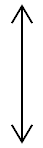
\includegraphics[width=0.06\textwidth]{figs/shapes/vertical_double_arrow.png}}& zhongsanyan & 4/4 & \multirow{5}{*}{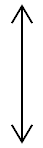
\includegraphics[width=0.06\textwidth]{figs/shapes/vertical_double_arrow.png}} \\
& kuaisanyan & 4/4 & \\
& yuanban & 2/4 & \\
& erliu & 2/4 & \\
& liushui & 1/4 & \\
fast & kuaiban & 1/4 & syllabic \\
\bottomrule
\end{tabular}
\caption{Jingju metred banshi.}
\label{tab:banshi}
\end{table}

The primary or original banshi is called 原板 (pinyin: yuanban), with time signature 4/4. When it is transformed into 1/4, the corresponding banshi is 快板 (pinyin), and the tempo is also accelerated. When yuanban is transformed into 4/4, the resulting banshi is 慢板 (pinyin: manban), meaning slow banshi. When yuanban is transformed into manban, not only the time duration of syllables are extended, but also the number of ornamentations within each syllable are increased. However, when yuanban is converted to kuaiban, the singing style becomes almost syllabic -- one beat for one syllable. 

三眼 (pinyin: sanyan, literally translated as three eyes) is another name for manban. Sanyan banshi can be divided into three sub-banshi -- 慢三眼 (mansanyan, equal to manban), 中三眼 (zhongsanyan), 快三眼 (kuaisanyan). The tempo of kuaisanyan is faster than zhongsanyan, and they both faster than mansanyan but slower than yuanban. Except for yuanban, the banshi of time signature 2/4 category also contain 二六 (pinyin: erliu, literally translated as two six) because their couplet has six accented beats. In terms of shengqiang xipi, there is another metred banshi -- 流水 (pinyin: liushui, literally running water) which uses 1/4 time signature, is faster than yuanban but slower than kuaiban. We list major jingju metred banshi in \tabref{tab:banshi}.

Three main unmetred banshi are 导板 (daoban), 回龙 (huilong) and 哭头 (kutou). Daoban is the first melodic line of a chang duan. Huilong follows daoban, and is used to draw out the metred banshi. Kutou, literally crying head, is used for a grievous outburst and can occur after any section of the couplet. The variety of banshi is needed to convey the emotional content of the lyrics. In general, yuanban is related to neutral and narrative lyrics content; manban reflects introspective, and deep emotions; while kuaiban expresses agitation, nervousness.

The precise, clear pronunciation is critical to jingju listening comprehension, and also form an important aural aesthetic value of jingju. The primary focus of this dissertation is the pronunciation aspect of jingju singing. An in-depth description of jingju pronunciation concepts is given in the following section.

\section{A review of automatic assessment of musical performance}
entire music excerpt, note, syllable, phoneme level
template based, model based

\subsection{Automatic assessment of musical performance}

We introduce the overview of the studies on general automatic assessment of musical performance in this seciton. In most of these studies, the assessment are conducted for the entire music excerpt. In the other studies, the assessment are performed at musical note-level. A significant number of authors adopt the regression or classification model to predict the human rating of the musical performance with acoustic features. We notice that most of the methods are template-based, meaning that the reference performance are provided for a comparision with the target assessing performance. While other methods are model-based, such that the reference performance are not given, and the target performance are assessment using a pre-trained model. In this following part of this section, we firstly present the studies of automatic singing voice assessment. Then we present those of instrumental performance assessment.

\subsubsection{Automatic assessment of singing voice}
In \tabref{tab:ch2_automatic_assessment_singing}, we list the goal and methods of each work. A model-based method is presented by \shortcite{Nakanoa} for evaluating unknown melodies. The SVM is trained with semitone stability and vibrato features to classify the good and poor singers. The evaluation dataset contains 600 songs sung by 12 singers -- 6 good and 6 poor. \shortcite{Daido2014a} identifies that three features -- A-weighted power, F0 fall-down and vibrato extent, are relevant to singing enthusiasm. Then they build a regression model to predict the human rating scores of singing enthusiam by combing these three features.

As we have mentioned above, most of the works are template-based and build regression or classification model for the prediction of human rating. \shortcite{Caoa} calculate features on four categories -- intonation, rhythm, timbre brightness and vocal clarity, then adopt SVR regression model to predict the expert rating scores of the singing quality. \shortcite{Liu2011a} propose a two-step method for solfège assessment. In the first step, they use DTW to align the reference and target performance pitch tracks. In the second step, they calculate intonation and rhythm features using the aligned musical notes. Relative pitch interval and lagged tempo reference are identified respectively as the most correlated features for intonation and rhythm rating. \shortcite{Tsai2012a} model intonation rating using DTW cost between reference and target pitch tracks, model volume rating using DTW cost between reference and target logarithmic energy curves, model rhythm rating using HMM classification score between pitch strength time sequences, and predict the overall score with linear regression model by combining these three dimension ratings. 

\shortcite{Molinaa} explore both low-level and high-level features for singing voice intonation and rhythm assessment. The reference used in their work is not symbolic midi but singing audio. Low-level features are calculated based on the DTW alignment path, and high-level features are calculated on the transcribed musical notes. They calculate the correlation coefficients between each individual feature and expert rating score, and find that low-level total intonation error and high-level pitch difference are correlated with the intonation rating and low-level RMS of the alignment path is correlated with the rhythm rating. Finally, they use quadratic polynominal regression model with all the features to predict the overall singing quality. \shortcite{Bozkurta} develop a dataset and a baseline model for the singing assessment of the conservatory entrance exam. Their dataset contains 2599 piano references and 1018 singing performance of 40 different melodies. These singing performances are labeled as pass or fail categories by 3 experts. They use DTW to align the pitch tracks between the singing performance and the piano reference. The baseline is built by using a multilayer perceptron model with 3 featuers -- pitch difference histogram, DTW alignment cost and the amount of the length change of the DTW alignment. \shortcite{Guptab} construct the singing assessment model on 6 aspects - intonation accuracy, rhythmic consistency, pronunciaiton, vibrato, volume and pitch range. To avoid the alignment error caused by the intonation mistake, they use MFCC as the representation for the DTW alignment between reference and target. They also experiment cognition modeling for obtaining the perceptual relevant features. Finally, both linear regression and multilayer perceptron models are explored to predict human ratings with various feature combinations.

In the works mentioned above, the model are built to assess the singing performance in the entire musical excerpt granularity. However, several works explore the assessment of detailed musical events, such as note, expression segment and syllable. \shortcite{Mayor2006b} proposed a probablistic and rule-based method for note alignment and expression segmentation. They use HMM framework with Viterbi algorithm for the note alignment. The cost probablity is calculated by a set of heurstic rules which are defined on timing, pitch, energy, vibrato and timbre. The similar idea is adopted for expression segmentation. They define several rules for the expressions such as attack, sustain, vibrato, release and transition. The HMM topology of the expression is constrained by the note segmentation. \shortcite{Schramm2015b} construct a Bayesian classifier to assess the performing correctness of solfège note. They first transcribe the pitch track and notes for the target singing performance, and devise a special DTW algorithm to align the reference score the transcribed notes. For each assessment dimension -- note-level pitch, onset and offset, they construct Gamma probability density functions for both correct and incorrect classes. Finally, they identify the fuzzy boundary between two classes using a Bayesian classifier. In \shortcite{Guptac}'s work, they first generalize the mispronounciation rules for the singing voice of Southeast Asian English dialects. Then they use Automatic Speech Recognition system with an adapted dictionary to detect the mispronunciation.

\begin{landscape}
\begin{table}[ht!]
\ContinuedFloat
\centering
\begin{tabular}{lcc}
\toprule
Authors              & Goal                                          & Methods                                                                                           \\
\midrule
\shortcite{Mayor2006b}  & Expression categorization and alignment       & \makecell{Rule-based note and\\expression alignment\\using Viterbi algorithm}         \\\hline
\shortcite{Nakanoa}     & \makecell{Singing skill evaluation\\for unknown melodies} & \makecell{Building SVM model\\to classify good and bad performance.}      \\\hline
\shortcite{Caoa}        & Singing quality evaluation                    & \makecell{Building SVM regression model\\between features and\\human rating scores.}  \\\hline

\shortcite{Liu2011a}    & Singing evaluation                            & \makecell{Using correlation coefficient\\to select the best features.}                \\\hline
\shortcite{Tsai2012a}   & Karaoke singing evaluation                    & \makecell{Building linear regression model\\for predicting the overall score.}        \\
\bottomrule   
\end{tabular}
\caption{Summary table of the previous studies on automatic assessment of singing voice.}
\label{tab:ch2_automatic_assessment_singing}
\end{table}
\end{landscape}

\begin{landscape}
\begin{table}[ht!]
\ContinuedFloat
\centering
\begin{tabular}{lcc}
\toprule
Authors              & Goal                                          & Methods                                                                                           \\
\midrule
\shortcite{Molinaa}      & Singing voice assessment              & \makecell{Building nonlinear regression model\\for predicting the human rating score.}                     \\\hline
\shortcite{Daido2014a}   & Singing enthusiasm evaluation         & \makecell{Building linear regression model\\for predicting the human rating\\of singing enthusiasm.}        \\\hline
\shortcite{Schramm2015b} & Solfège assessment                    & \makecell{Constructing Gamma probability\\density functions,\\building Bayesian classifiers\\for each note.}    \\\hline
\shortcite{Guptac}       & Singing mispronunciation detection    & \makecell{DNN-HMM lyrics-to-audio\\forced alignment,\\using an adapted dictionary\\to detect mispronunciation.} \\
\bottomrule   
\end{tabular}
\caption{Summary table of the previous studies on automatic assessment of singing voice. (continued)}
\end{table}
\end{landscape}

\subsubsection{Automatic assessment of intrumental music performance}

In \tabref{tab:ch2_automatic_assessment_instrumental}, we list the goal and methods of each work. We have identified that in three works, the assessment is conducted at music excerpt level. Several pitch and rhythm score-independent features and score-based features are proposed in \shortcite{Vidwans2017a}'s work. A SVR regression model is experimented with various feature combinations to predict the expert ratings of Alto Saxophone performance. \shortcite{Wua} use sparse coding to learn representations in a unsupervised way on the local histogram matrix features. The learned features are used in a SVR model to predict the expert ratings for the percussive music performance. \shortcite{Pati2018a} use fully-convolutional neural networks and covolutional recurrent neural networks to predict the expert ratings for the saxophone, clarinet and flute music performance. Pitch track and logarithmic Mel band energies are adopted as the input representations of the networks. They also discuss the learned representation for the musicality dimension using network inspection techniques. 

In other works, the asessment is done at musical note-level. \shortcite{Robinea} assess the note quality of saxophone performance. They extract pitch and amplitude related features for stable, crescendo/decrescendo and vibrato notes. Then, the feature values are mapped to the expert ratings. \shortcite{Knighta} develop models to assess the trumpet performance at note-level. They use a SVM classifier to predict the expert ratings with 56 dimensional features of which are mostly spectral features. \shortcite{Luoa} build a bag-of-features plus classifciation model to detect violin performing mistake. Their note and expression segmentation are achieved using a photo resistor and four rings of surfacemounted light-emitting diodes (SMD LEDs). \shortcite{Hana} detect three types of flute performing errors -- assembeling error, fluctuated sound and mis-fingering by using handcrafted features and Random Forest classifier.

\begin{landscape}
\begin{table}[ht!]
\centering
\begin{tabular}{lcc}
\toprule
Authors              & Goal                                          & Methods                                                                                           \\
\midrule
\shortcite{Robinea}  & To assess saxophone notes                     & \makecell{Extracting metrics for straight,\\crescendo/decrescendo\\and vibrato notes}                         \\\hline
\shortcite{Knighta}  & Trumpet tone quality assessment               & \makecell{Building SVM model\\to classify trumpet tone quality on 7 scales.}                                  \\\hline
\shortcite{Hana}     & \makecell{Detecting common mistakes\\of flute players}       & \makecell{Using handcrafted features, thresholding\\and Random Forest classifier\\to detect playing mistakes.} \\\hline
\shortcite{Luoa}     & \makecell{Detection of common violin\\playing mistakes}      & \makecell{Building SVM classifiers\\for detecting four types\\of violin playing mistakes.}      \\\hline
\shortcite{Vidwans2017a}         & \makecell{Assessment of student\\music performance}          & \makecell{Building SVR regression model\\for predicting the human rating score.}    \\\hline 
\end{tabular}
\caption{Summary table of the previous studies on automatic assessment of instrumental musical performance.}
\label{tab:ch2_automatic_assessment_instrumental}
\end{table}
\end{landscape}

\begin{landscape}
\begin{table}[ht!]
\ContinuedFloat
\centering
\begin{tabular}{lcc}
\toprule
Authors              & Goal                                          & Methods                                                                                           \\
\midrule
\shortcite{Bozkurta}         & Singing voice assessment                      & \makecell{Building a Multilayer perceptron model\\for predicting the human rating.}                         \\\hline
\shortcite{Guptab}           & Singing quality evaluation                    & \makecell{Using both linear regression\\and Multilayer perceptron\\for predicting the human rating.}        \\\hline
\shortcite{Wua}           & \makecell{Percussive\\music performance assessment}        & \makecell{Using sparse coding to learn the feature,\\then building SVR modelfor prediction.}                 \\\hline
\shortcite{Pati2018a}           & Student music performance                     & \makecell{Using fully-convolutional network\\or covolutional recurrent network\\for prediction.}           \\
\bottomrule   
\end{tabular}
\caption{Summary table of the previous studies on automatic assessment of instrumental musical performance. (continued)}
\end{table}
\end{landscape}

\subsection{Musical onset detection}

\subsection{Lyrics-to-audio alignment and lyrics recognition}

\subsection{Neural acoustic embeddings}
\chapter[Automatic assessment of singing voice pronunciation of jingju music
]{Automatic assessment of singing voice pronunciation of jingju music
}\label{chap:probdef}
% \begin{epigraphs}
% \qitem{A problem well stated is a problem half-solved}{Charles Kettering}
% \qitem{The formulation of the problem is often more essential than its solution, which may be merely a matter of mathematical or experimental skill}{Albert Einstein}
% \end{epigraphs}

Automatic assessment of singing voice of jingju music has not been explored systematically, which means that the challenges, opportunities and relevant research problems have not been formally studied. This chapter presents the attempts to open up this research topic. We first elucidate the important role of pronunciation played in jingju singing training. Then we introduce several relevant research problems, with a review of the start of the art for jingju music or other music traditions in the context of CompMusic project. We the background of all the relevant research problems, we formulate the thesis problems of syllable and phoneme segmentation, mispronunciation detection for special pronunciation, and pronunciation similarity measures at phoneme level. The main objectives of the chapter are:

\begin{enumerate}[leftmargin=*]
	\item To present, and discuss the role of pronunciation in jingju singing training.
	\item To identify, present, and discuss main challenges to automatic assessment of singing voice pronunciation in jingju music.
	\item To identify, present, and discuss main opportunities in automatic assessment of singing voice pronunciation in jingju music
	\item To identify several relevant research problems within the context of jingju music and identify key challenges in addressing them, as a way to indicate future work in singing voice assessment.
	\item From the relevant problems, identify a subset of research problems and formulate them in detail, to be addressed in the scope of this dissertation.
\end{enumerate}
%
\section{The role of pronunciation in jingju singing training}\label{sec:probdef:role_pronunciation}

Assessment of singing performance can be conducted in various musical dimensions such as intonation, rhythm, loudness, tone quality and pronunciation. The automatic assessment method can be devised either for a special dimension or the overall performing quality \cite{Guptab}. Due to the various and complicate conventions existed in jingju singing performance, and also the strictness of jingju singing training, the automatic system conceived for the assessment of jingju singing needs to have the ability to judge the performance in each dimension. However, due to time and energy constraints, it is not possible to address the relevant research problems of all the musical dimensions in this dissertation. 

In this section, we attempt to answer the question: how the jingju singing teachers and students value the importance of each musical dimension? By answering this question, we can identify the most important dimension consistently considered by teachers and students -- pronunciation.

\subsection{Jingju singing training and correction occurrence}\label{sec:probdef:correction_occurance}

Jingju singing is traditionally taught between teacher and student by using the mouth/heart (oral teaching, 口传心授) and face-to-face methods—“Jingju tuition requires demonstration, and teachers tell students the secrets for certain skills that they learned from their masters or that they worked out from their experience. The close relationship of the teacher-student or the master-disciple is based on the mouth/heart teaching method that stresses through oral instruction and intuitive understanding. Imitation is certainly the first step, and it is crucial for our learning process… not even one component in the `four skills (singing, speech, dance-acting, combat)' can be learned by the student himself. Much of the nuance of the singing can only be learned from face-to-face teaching.” \cite{Li2010a}

\begin{figure}[ht!]
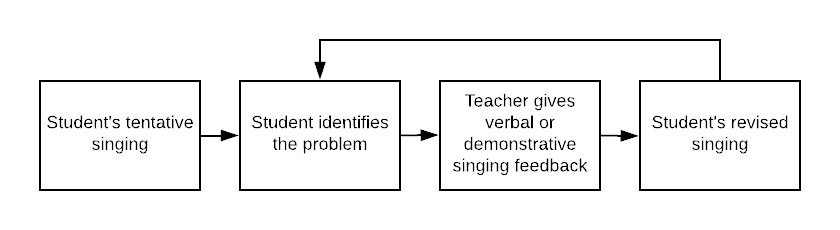
\includegraphics[width=\textwidth]{figs/blockDiags_rong/ch3_occurrance_flow.png}
\caption{The flowchart of a single correction occurrence.}
\label{fig:ch3_occurrance_flow}
\end{figure}

After five months research stay in NACTA (National Academy of Chinese Theatre Arts, leading institute in China dedicated to the training of professionals in performing and studying traditional Chinese opera), we had a firsthand experience of the month/heart teaching method of jingju singing. In class, the teacher teaches several melodic lines selected from an aria. In the first part of the class, the teacher gives a short introduction to the teaching content such as the story and the character setting of the aria, the special pronunciations. Then she/he gives a demonstrative singing of these lines. In the second part of the class, the students imitate the demonstrative singing line by line, and the teacher corrects the imitations. The process of the second part can be generalized as (i) the teacher asks the students to give a tentative singing individually at melodic line-level, or syllable-level. (ii) Then the teacher identifies the singing problems, (iii) gives verbal or demonstrative singing feedback. (iv) Finally, the students do a revised singing with the feedbacks in mind. The step from (ii) to (iv) could be iterated until the student's singing satisfies the teacher's criteria. We name one single such process as a correction occurrence (see \figref{fig:ch3_occurrance_flow}).

The verbal feedback is a semantic comment given by the teacher. It is the description that is aimed to help the student to improve her/his singing performance, and it is the most valuable information which can clarify the singing problems.

In paper \cite{geringer_musicians_1998}, the musicians have rated the performance of western arias in 5 musical dimensions: phrasing/expression, intonation, rhythm, loudness, tone quality. In our study, we borrow the concept of musical dimensions for music performance assessment and adapt them according to jingju singing background. 

Almost all jingju aria contains lyrics, and as we will prove in later chapters -- to be able to pronounce the singing lyrics accurately is a key skill in jingju singing, we thus add the pronunciation as an independent dimension to the dimension set mentioned above. Besides, we discard phrasing/expression because it is a ``meta-dimension" constructed above other basic dimensions -- ``A musician accomplishes this by interpreting the music, from memory or sheet music, by altering tone, tempo, dynamics, articulation, inflection, and other characteristics"\footnote{\url{https://en.wikiquote.org/wiki/Musical_phrasing} Retrieved 25 July 2018}. Overall, 5 dimensions will be taken into account in this paper -- intonation, rhythm, loudness, tone quality and pronunciation. Accordingly, we give their definitions:

\begin{itemize}
	\item Intonation: accuracy of pitch in singing.
	\item Rhythm: singing a rhythmic pattern on time, which means that the notes or syllable are not ahead of the time or behind the time.
	\item Loudness: the dynamic loudness variation between notes/syllables or phrases.
	\item Tone quality: the color or timbre of the singing voice.
	\item Pronunciation: the act or result of producing the sounds of speech, including articulation and stress.
\end{itemize}

In the next section, we explain our methods -- classifying teachers' correction occurrence and surveying the students. These methods aim to answer the question: how teachers and students value the importance of each jingju singing dimensions -- intonation, rhythm, loudness, tone quality and pronunciation. By classifying the correction occurrences, we will find out the dimensions on which teachers lay stress or students tend to have problems. On the other hand, we conduct a simple survey to investigate the importance of each dimension from the students' perspective.

\begin{figure}[ht!]
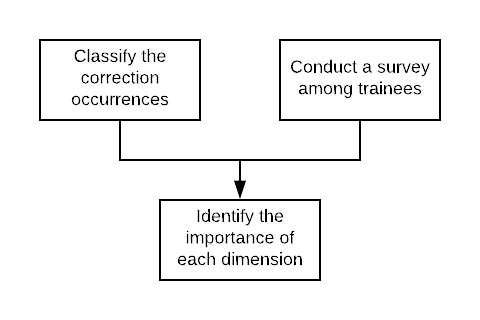
\includegraphics[width=\textwidth]{figs/blockDiags_rong/ch3_occurrance_analysis_flow.png}
\caption{The flowchart of the dimension importance identification process.}
\label{fig:ch3_occurrance_analysis_flow}
\end{figure}

\subsubsection{Correction occurrence analysis}\label{sec:ch3:correction_analysis}

During the research stay in NACTA, we audited and recorded the audio from three singing classes. Three class was taught respectively by three professional teachers, which contain solo and chorus practices. We recorded the class teaching and practicing audio content by using a SONY PCM-D50 stereo portable audio recorder. Only the solo practices are kept for the analysis because they can reveal the singing problems of an individual student, whereas the individual voices are blurred in the chorus practice recordings. The audio excerpts of each correction occurrence are then edited and visualized by signal processing tools—pitch contour, loudness contour and spectrogram, which is helpful in identifying the singing problem, especially when the teacher's verbal feedback is too abstract to extract any effective information. 

\begin{table}[ht!]
\centering
\begin{tabular}{ccccc}
\toprule
Aria name              & Role-type     & \makecell{\#Student} & \makecell{\makecell{\#Melodic\\line}} & \makecell{\makecell{\#Correction\\occurrence}} \\
\midrule
\makecell{武家坡\\WuJiaPo}          & laosheng & 3              & 11                  & 20                           \\
\makecell{太真外传\\TaiZhen\\WaiZhuan} & qingyi   & 3              & 3                   & 21                           \\
\makecell{捉放曹\\ZhuoFang\\Cao}      & hualian  & 2              & 28                  & 21                       \\
\bottomrule
\end{tabular}
\caption{The statistics of the correction occurrence analysis materials.}
\label{tab:correction_occurrence_stat}   
\end{table}

\tabref{tab:correction_occurrence_stat} depicts the information of aria name, role-type, student number in the class, melodic line number practiced in the class and correction occurrence number collected from the recordings. An example of reading this table is ``Three students were involved in the laosheng class WuJiaPo. 11 melodic lines were taught, and 20 correction occurrences were collected from the recordings".

The ratios between the melodic line number and the correction occurrence number are widely different for the three classes (\tabref{tab:correction_occurrence_stat}). For example, during the TaiZhenWaiZhuan class, three students practiced three lines and were corrected 21 times, which results in a ratio of 1/7. However, during the ZhuoFangCao class, two students practiced 28 lines and also were corrected 21 times, which has a ratio of 4/3. The correction frequency depends on several factors, such as the students' singing levels, the teacher's teaching method. The low singing level students tend to receive more corrections than those who have high singing levels.

For each occurrence, we analyze the target recordings and the teacher's verbal feedback. Additionally, to achieve the visual analysis, their pitch, loudness contours and spectrogram are also presented.

We firstly classify the correction occurrences into five dimensions—intonation, rhythm, loudness, tone quality and pronunciation. A correction occurrence can be classified into more than one dimension. For example, the correction with the verbal feedback “don't be sloppy, sing it with solidity, make the tone quality sounds round.” can be classified into intonation (irregular vibrato), loudness (unstable loudness contour) and tone quality (higher harmonics too clear), by analysing comparatively between the teacher's demonstrative singing and student's tentative singing. Furthermore, a finer inspection of each correction occurrence is conducted, where we identify the detailed elements.

Five correction occurrences are taken as examples to showcase our analysis. For each one, we list its aria name, melodic line, target syllable, the teacher's verbal feedback, the dimensions classified. Finally, we give a short explanation accompanied by the visualization to justify our classification process.

\begin{figure}[ht!]
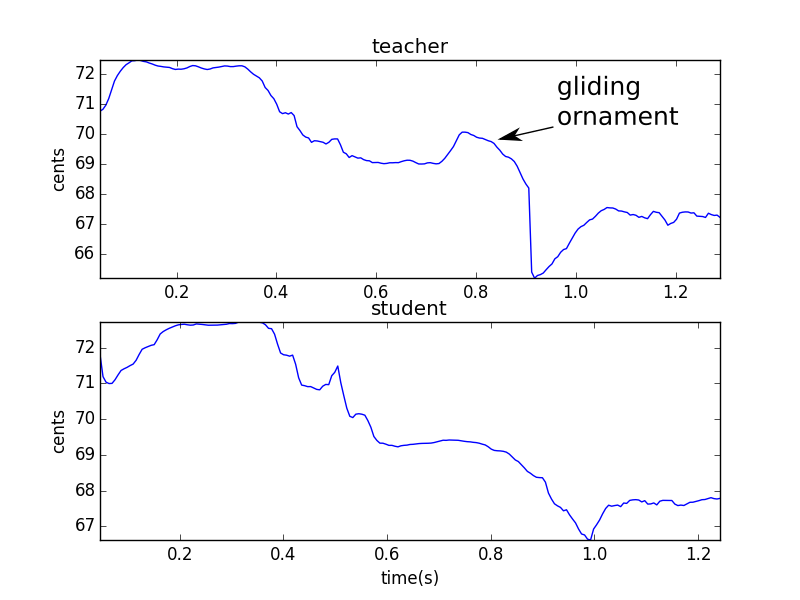
\includegraphics[width=\textwidth]{figs/spectro_vis/ch3_occ1.png}
\caption{The pitch contours of the syllable ``yuan" for occurrence 1.}
\label{fig:occurrence_1}
\end{figure}


\noindent\textbf{Occurrence 1:}

\begin{itemize}[leftmargin=*, noitemsep]
\item Aria: TaiZhenWaiZhuan (太真外传)
\item Line: yi yuan na chai yu he qing yuan yong ding (一愿那钗与盒情缘永定)
\item Target syllable: yuan (缘)
\item Teacher's verbal feedback: it didn't jump up. (没跳起来) 
\item Dimension: intonation
\item Explanation: The syllable's second tone in the teacher's demonstrative singing has a pitch gliding (ornament). However, the gliding in the student's version is not apparent (\figref{fig:occurrence_1}).
\end{itemize}

\begin{figure}[ht!]
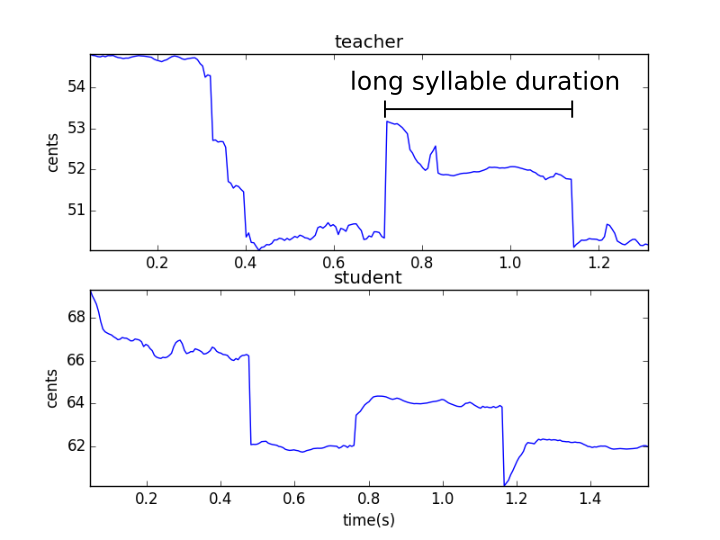
\includegraphics[width=\textwidth]{figs/spectro_vis/ch3_occ2.png}
\caption{The pitch contours of the syllables ``dang nian jie bai" for occurrence 2.}
\label{fig:occurrence_2}
\end{figure}

\noindent\textbf{Occurrence 2:}

\begin{itemize}[leftmargin=*, noitemsep]
\item Aria: ZhuoFangCao (捉放曹)
\item Line: dang nian jie bai yi lu xiang (当年结拜一炉香)
\item Target syllables: dang nian jie bai (当点结拜)
\item Teacher's verbal feedback: swing apart these four syllables (1,2,3,4 四个字甩开)
\item Dimension: rhythm
\item Explanation: In teacher's demonstrative singing, the temporal duration of the third syllable ``jie" has been prolonged, in contrast with the other three syllables, which can be observed by the pitch contour (\figref{fig:occurrence_2}).
\end{itemize}

\begin{figure}[ht!]
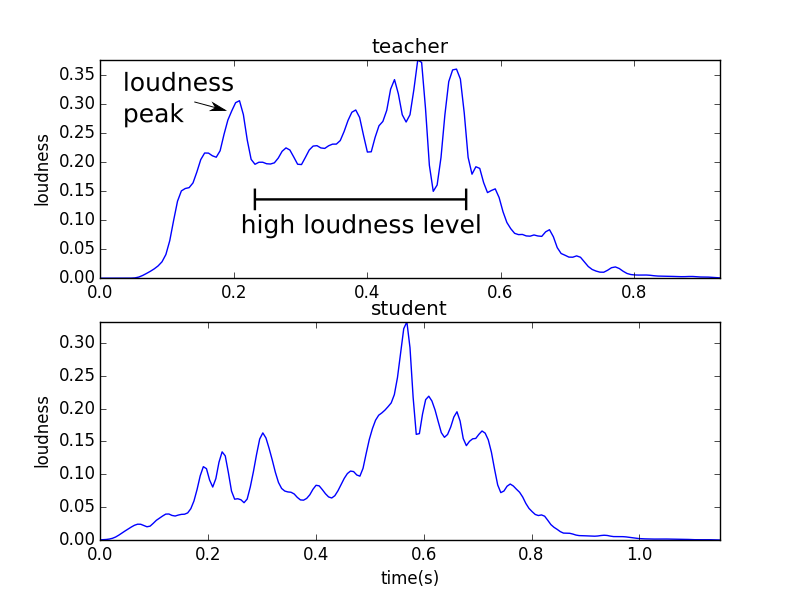
\includegraphics[width=\textwidth]{figs/spectro_vis/ch3_occ3_1.png}
\caption{The loudness contours of the syllable ``yang" for occurrence 3.}
\label{fig:occurrence_3_1}
\end{figure}

\begin{figure}[ht!]
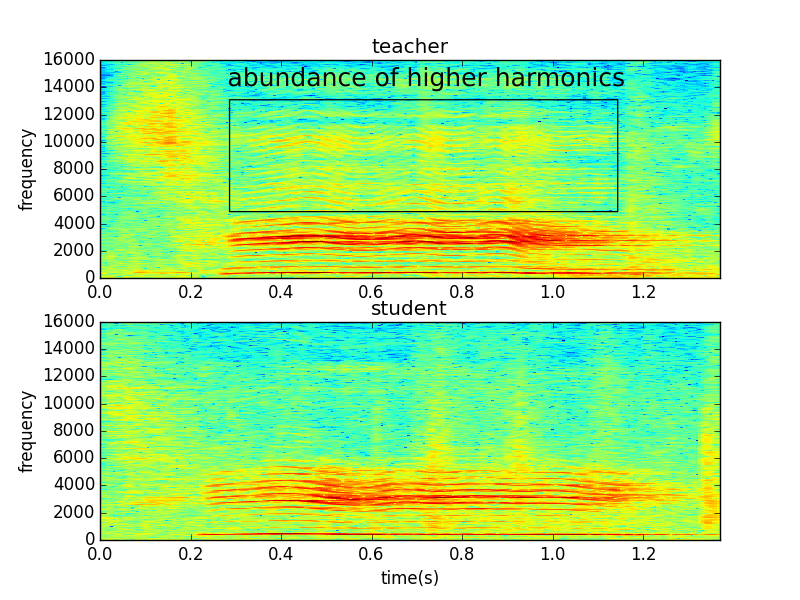
\includegraphics[width=\textwidth]{figs/spectro_vis/ch3_occ3_2.png}
\caption{The spectrograms of the syllable ``yang" for occurrence 3.}
\label{fig:occurrence_3_2}
\end{figure}

\noindent\textbf{Occurrence 3:}

\begin{itemize}[leftmargin=*, noitemsep]
\item Aria: TaiZhenWaiZhuan (太真外传)
\item Line: yang yu huan zai dian qian shen shen bai ding (杨玉环在殿前深深拜定)
\item Target syllable: yang (杨)
\item Teacher's verbal feedback: emphasizing the nasal voice (an 鼻音要突出)
\item Dimensions: loudness and tone quality
\item Explanation: In teacher's demonstrative singing, a prominent loudness peak can be found in the head of the syllable, which maintains a high loudness level in the belly (\figref{fig:occurrence_3_1}). We also can observe that the higher harmonics are abundant from the spectrogram (\figref{fig:occurrence_3_2}).
\end{itemize}

\begin{figure}[ht!]
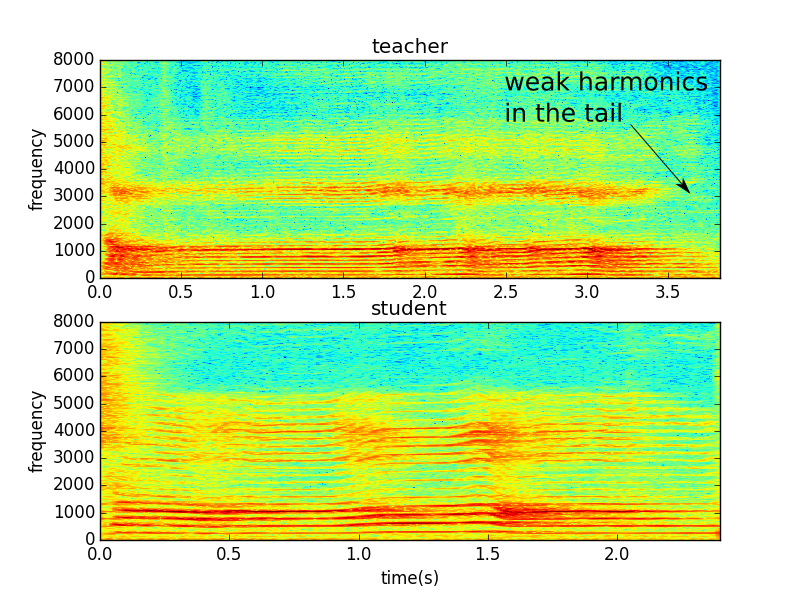
\includegraphics[width=\textwidth]{figs/spectro_vis/ch3_occ4.png}
\caption{The spectrograms of the syllable ``shang" for occurrence 4.}
\label{fig:occurrence_4}
\end{figure}

\noindent\textbf{Occurrence 4:}

\begin{itemize}[leftmargin=*, noitemsep]
\item Aria: ZhuoFangCao (捉放曹)
\item Line: xian xie zuo le na wa shang shuang (险些做了那瓦上霜)
\item Target syllable: shang (上)
\item Teacher's verbal feedback: terminate the sound at /ng/ (sound收音收到 ng)
\item Dimension: pronunciation
\item Explanation: The teacher's demonstrative singing is one octave lower than the student's singing. The teacher's feedback emphasizes the pronunciation quality of the syllable tail sound -- /ng/. His demonstrative singing contains fewer harmonics in the tail than the student's singing (\figref{fig:occurrence_4}).
\end{itemize}

\begin{figure}[ht!]
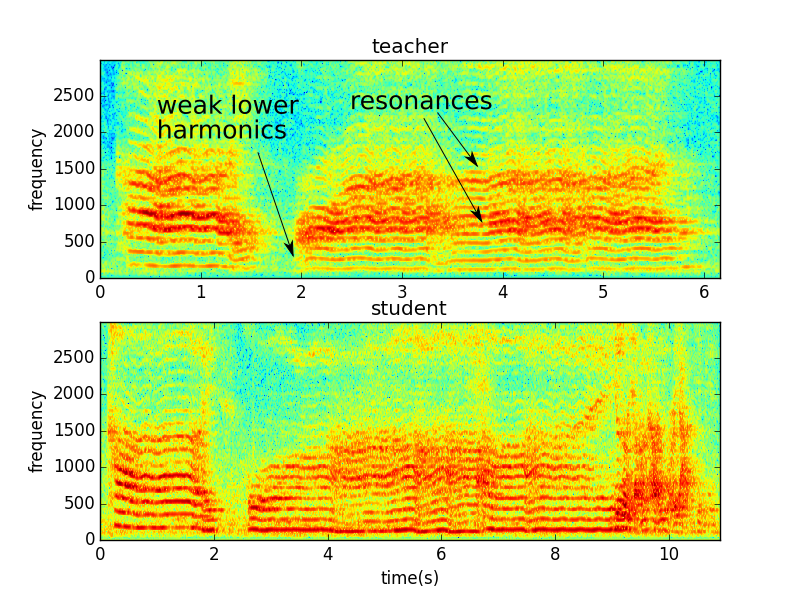
\includegraphics[width=\textwidth]{figs/spectro_vis/ch3_occ5.png}
\caption{The spectrograms of the syllables ``kai huai" for occurrence 5.}
\label{fig:occurrence_5}
\end{figure}

\noindent\textbf{Occurrence 5:}

\begin{itemize}[leftmargin=*, noitemsep]
\item Aria: WuJiaPo (武家坡)
\item Line: jian liao na zhong da sao xi wen kai huai (见了那众大嫂细问开怀)
\item Target syllable: kai huai (开怀)
\item Teacher's verbal feedback: adjust the breath, make the sound solid even if you sing in the low register (要用气,低调们也要放实在了)
\item Dimension: tone quality
\item Explanation: This feedback has twofold of meaning. First is to take enough breath, and have enough air in the chest to sing. Second is to adjust the body's resonance position to make the sound more solid. This can be observed as in the spectrogram of the teacher's demonstrative singing, which contains less energy for the lower harmonics and the prominent resonances (energy) in around 750 Hz and 1250 Hz (\figref{fig:occurrence_5}).
\end{itemize}

\subsubsection{A survey among students}
We conduct a simple survey of another nine students to investigate the importance of each dimension from their perspectives. The survey contains two questions: 

Please rate the use frequency of the following media when you learn to sing arias -- score, audio recording or teacher's classroom teaching. 
Please rate the importance of the following jingju singing dimensions and elements when you learn to sing arias—intonation, rhythm, loudness, pronunciation, ornament, breath and strength (劲头). 

Nine students have participated in this survey; they are different from the ones presented in \secref{sec:ch3:correction_analysis}. Among them, five are professional undergraduate students or students already graduated from NACTA, four are amateurs from the jingju associations in two non-art universities in Beijing. We use a five-level Likert scale for each rating term. For example, the ``use frequency of the score" in the first question and the ``importance of intonation" in the second question can be rated from 1 to 5, where 1 means ``never used" or ``not important at all" and 5 means ``most frequently used" or the ``most important". Then, we take the average value of each term for five professional students and four amateurs respectively. 

It is worth to mention that three more elements -- ornament, breath and strength have been added to the survey. The consideration for this change is that the survey terms need to be adapted to the student's artistic background, and the jingju singing jargons should be easily accessible by them.

\subsection{Results and discussion}

In this section, we report the results of the analysis of teachers' correction occurrences and the students' survey. The correction occurrences are classified into five dimensions by using the method introduced in the \secref{sec:probdef:correction_occurance}. Then, we discuss the student' survey result and compare it with the teachers' correction occurrence classification result.

\subsubsection{Correction occurrence analysis}\label{sec:ch3:correction_occurrence_results}

\begin{table}[ht!]
\centering
\begin{tabular}{cccccc}
\toprule
              & Inton.     & Rhythm & Loud. & Pronun. & \makecell{Tone\\quality} \\
\midrule
\makecell{武家坡\\WuJiaPo}          		& 8 	& 0 & 1 	& 6		& 6 \\
\makecell{太真外传\\TaiZhen\\WaiZhuan} 	& 6   	& 1 & 9 	& 4     & 11 \\
\makecell{捉放曹\\ZhuoFangCao}      		& 5  	& 2 & 7 	& 9     & 3 \\
Sum 									& 19 	& 3	& 17 	& 19	& 20 \\
\bottomrule
\end{tabular}
\caption{The statistics of the correction occurrence dimension classification. Inton.: intonation; Loud.: loudness, Pronun.: pronunciation.}
\label{tab:correction_occurrence_dimension_classification}   
\end{table}

We observe from the \tabref{tab:correction_occurrence_dimension_classification} that among the five dimensions, tone quality, pronunciation and intonation dimensions have the largest and almost equal occurrence number, loudness takes the second place, and rhythm problem was least mentioned. In other words, tone quality, pronunciation and intonation are the dimensions which receive particular attention from teachers and cause problems easily to students.

The correction occurrence analysis results are organized in an Excel spreadsheet, which consists of the teacher's verbal feedback, signal analysis method, and classified dimension.

\subsubsection{The survey among students}

We gather the survey results by ordering the mean values for each question. For the first question, the usage frequency ordered from high to low of three learning media are: 

\begin{enumerate}[noitemsep]
\item Professional group: classroom teaching, audio recording, score;
\item Amateur group: audio recording, teacher's classroom teaching, score. 
\end{enumerate}

The music score has been rated as the lowest use frequency by both professional and amateur groups, which means that the jingju students we investigated do not use the visual clue -- music score reading, to learn arias. The teacher's classroom teaching has been rated as the highest use frequency for the professional and the second for the amateurs, which is reasonable because this learning medium is much easier available for the professional. Lastly, the high rating of both teacher's classroom teaching and audio recording shows that the jingju students use mostly the listening and imitation methods to learn arias.

For the second question, the importance order from the most important to most trivial are: 

\begin{enumerate}[noitemsep]
\item Professional group: rhythm, strength, pronunciation, breath, intonation, loudness, ornament; 
\item Amateur group: rhythm, pronunciation, strength, ornament, breath, intonation, loudness. 
\end{enumerate}

Apart from the terms strength and breath, the others have been analyzed in the correction occurrence perspective. Strength is a stylistic and abstract word to depict the energy used in jingju singing and instrument playing. A jingju singing with strength is conveyed by combining multiple elements, such as loudness (mostly), rhythm, intonation and tone quality. Breath or specific methods of breathing (气口) described in Wichmann's book \cite{Wichmann1991a} is ``these methods allow the exiting breath to control the pitch, timbre or tone color, and energy of the sound produced." In consequence, Strength and breath both are nonspecific terms combining or affecting multiple basic jingju singing elements.

Pronunciation is rated as an essential element by both the professional and amateurs, which is coherent with the result of the correction occurrence analysis. The high importance of rhythm and low importance of intonation and loudness contradict to the result of the correction occurrence analysis. For rhythm aspect, one possible explanation is that the higher importance the students value a singing dimension, less prone they are going to sing poorly on it. For example, the students consider that rhythm is the most important singing aspect, they pay much attention to it during the practice. Thus they are less prone to have the rhythmic problems. For intonation and loudness, we cannot easily conclude that they are not important in the learning process. The reasons are twofold: on the one hand, the students might think that the intonation accuracy is a basic requirement in jingju singing and its importance is self-evident; on the other hand, because intonation and loudness are jargons used in acoustic, sound and music technology research fields, which might be foreign to these students, so they might avoid them and choose the familiar terms such as strength.

The only jingju singing dimension emphasized in both correction occurrence analysis, and the survey analysis is pronunciation, which shows that its crucial role in jingju singing training. As a consequence, to take advantage of limited time and effort, we will focus on tackling the research problems related to the assessment of singing pronunciation. In the following sections of this chapter, we present challenges, opportunities and research problems which are only related to the pronunciation dimension.

\section{Challenges and opportunities}

Significant challenges are existed to the automatic assessment of singing voice pronunciation in jingju music. We present and discuss challenges and opportunities from the perspectives of jingju singing characteristics and state of the art. These challenges will help us to formulate the research problems to be more comprehensive and akin to jingju music tradition. The opportunities, in turn, help us to pursue new MIR research directions. 

\subsection{Characteristics of jingju singing}\label{sec:ch3:char_singing}

We illustrate some signal characteristics of jingju singing voice that will be helpful to identify challenges for automatic assessment. 

\begin{landscape}
\mbox{}\vfill
\begin{figure}[ht!]
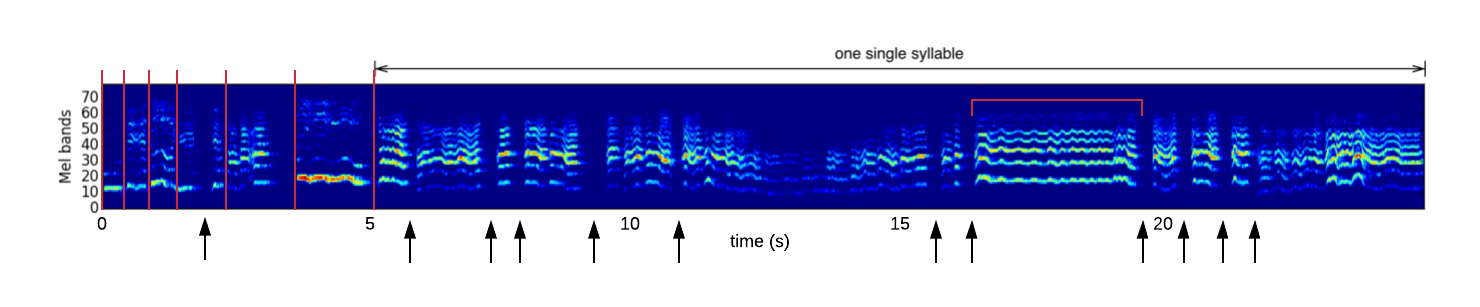
\includegraphics[width=1.8\textwidth]{figs/spectro_vis/ch3_jingju_char.png}
\caption{An example of a dan role-type singing phrase. Red vertical lines indicate the syllable onset time positions. Black arrows at the bottom specify the time positions of pause within the syllable. Red horizontal bracket shows a prominent singing vibrato.}
\label{fig:jingju_char}
\end{figure}
\vfill
\end{landscape}

\figref{fig:jingju_char} shows an example of a \textit{dan} role-type singing phrase in which the last syllable lasts approximately 20 seconds. This singing method -- 拖腔 (pinyin: tuoqiang, literally translated as the prolonged melody), used more commonly in \textit{dan} than in \textit{laosheng} singing, extends the duration of last syllable of the melodic line or a dou (\secref{sec:ch2:lyrics_structure}). It is a way of improving artistic expression, and the prolonged syllable can be used to carry various singing skills which include breath, intonational and dynamic control techniques, among others. 

In jingju singing, the breath must be under purposeful control at all times \cite{Wichmann1991a}. 偷气 (pinyin: touqi, stealing breath) is one of the primary methods to taking the breath in jingju singing. Performer inhales rapidly without exhaling beforehand. Touqi is performed when a sound is too long to be delivered in one breath and should be undetectable to the audience \cite{Wichmann1991a}. However, this is not the only technique which can lead to pauses within a syllable. Another singing technique (\textit{zu yin}, literally translated as block sound), provokes also pauses without occurring exhalation or inhalation. This kind of pause can be very short in duration and can be easily found in jingju singing syllables. 

Vibrato (颤音 chanyin and 波浪音 bolangyin) is extremely important in jingju singing such that a single pitch is rarely prolonged without a vibrato. Compared to the Western opera, jingju singing vibrato is slower and wider regarding vibrato rate and extent \cite{Yang2015a}. 

\begin{figure}[ht!]
    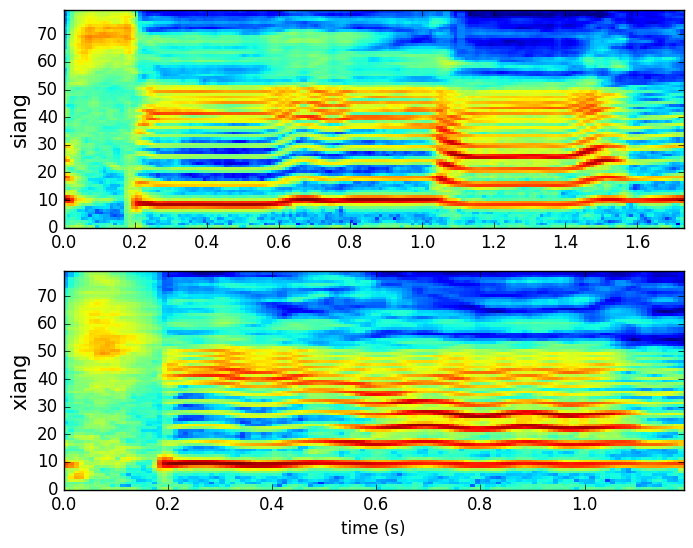
\includegraphics[width=\textwidth]{figs/spectro_vis/ch3_jianzi_mispronunciation.png}
    \caption{The Mel spectrograms of pointed syllable (jianzi) ``siang" and its corresponding rounded syllable (tuanzi) ``xiang".}
    \label{fig:ch3:jianzi_mispronunciation_example}
\end{figure}

\begin{figure}[ht!]
    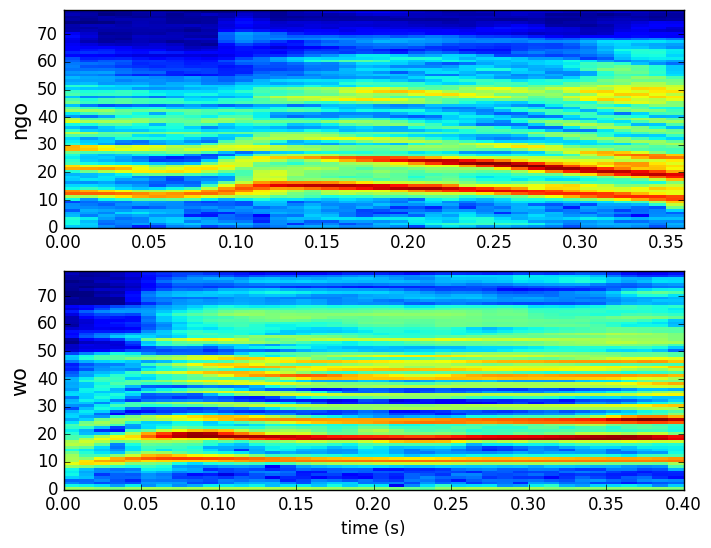
\includegraphics[width=\textwidth]{figs/spectro_vis/ch3_special_mispronunciation.png}
    \caption{The Mel spectrograms of the special pronounced syllable ``ngo" and its corresponding normal pronounced syllable ``wo".}
        \label{fig:ch3:special_mispronunciation_example}
\end{figure}

In jingju singing training, correctly pronouncing each written-character (syllable) is essential. The important role of pronunciation in jingju singing training has been discussed in \secref{sec:probdef:role_pronunciation}. However, in the actual training scenario, the student is likely to commit the pronunciation errors regarding two types of syllable -- jiantuanzi and special pronunciation, where their definitions have been introduced in \secref{sec:ch2:jiantuanzi} and \secref{sec:ch2:special_pronunciation}. Jiantuanzi mispronunciation means that the student mispronounces a pointed sound syllable (jianzi) as the rounded sound (tuanzi). The mispronunciation of the special syllables means that the student mispronounces a special pronounced syllable as the standard pronunciation in Chinese Mandarin. \figref{fig:ch3:jianzi_mispronunciation_example} and \figref{fig:ch3:special_mispronunciation_example} shows the Mel spectrograms of the mispronounced syllables. We can observe that the spectral difference between jianzi ``siang" and its corresponding tuanzi ``xiang" mainly lies in the non-voiced consonant part, and the difference between special pronounced syllable ``ngo" and its corresponding normal pronunciation ``wo" also lies in the syllable head part. The mispronunciation in jingju singing training and the formulation of the problem of mispronunciation detection will be continued to discuss in \secref{sec:ch3:mispronunciation_challenge} and \secref{sec:ch3:mispronunciation}.


\begin{figure}[ht!]
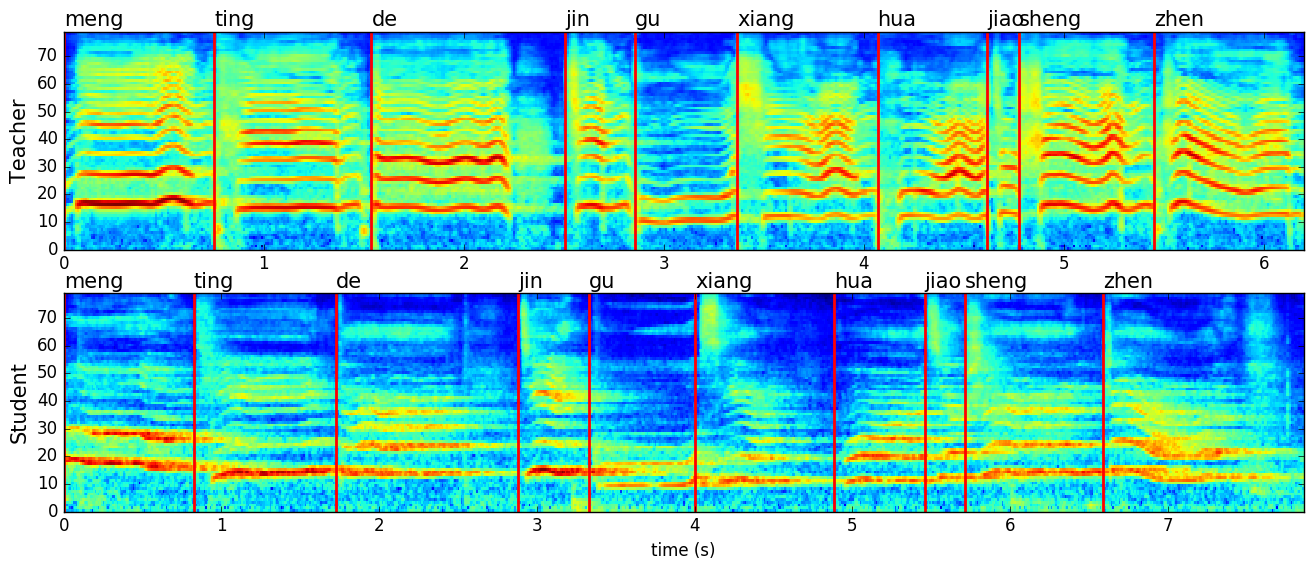
\includegraphics[width=\textwidth]{figs/spectro_vis/ch3_overall_qua.png}
\caption{The Mel spectrograms of teacher and student singing the same phrase ``meng ting de jin gu xiang hua jiao sheng zhen (in pinyin format)". Red vertical lines are the onset time positions of each syllable.}
\label{fig:overall_qua}
\end{figure}


The overall quality of the singing syllable or phoneme can be easily illustrated by using spectrogram. \figref{fig:overall_qua} shows the Mel spectrograms of a dan role-type singing phrase taken from the aria 猛听得金鼓响画角声震--《霸王别姬》 (meng ting de jin gu xiang hua jiao sheng zhen -- Farewell My Concubine). The upper part of the figure is the spectrogram of the teacher's recording, while the lower part is that of a primary school student's recording. Although the student does not commit any mispronunciation, there still exists a significant gap between the overall quality of her singing and that of the teacher singing. The gap is reflected in many aspects if we compare the two spectrograms. For example, the higher harmonics of the student singing is much weaker than those of the teacher; The consonants energies of the student singing are weaker than those of the teacher if we compare the consonants of syllables ``xiang" and ``sheng"; The intonation of the student singing is flat and lacks variation. 

\subsection{Challenges}\label{sec:ch3:challenges}

The basic music event of jingju singing is syllable. In jingju singing training, the accurate rendition of the syllabic pronunciation is placed in a more important position than that of the melody. In jingju circle, there is a saying 依字行腔 (pinyin: yi zi xing qiang, literally translated as singing according to the syllables), meaning that the singing melody should be consistent with the syllable tone and pronunciation, which also shows the importance of an accurate syllabic pronunciation. In \secref{sec:ch2:jingju_syllable}, we presented the structures and the lower-level components of jingju singing syllable. A jingju singing syllable consists of four types of phoneme -- an initial consonant or semivowel (optional), a medial vowel (optional), a central vowel and a tail (optional). As a consequence, at a more elaborate level, to pronounce a jingju syllable accurately is to render these elementary phonemes accurately.

According to the jingju singing principles mentioned above, to assess a jingju singing pronunciation at syllable or phoneme level, an automatic assessment system of jingju singing needs to have the ability to segment the singing recording automatically into the syllabic or phonetic unit. As we have mentioned in \chapref{chap:bkgnd}, a jingju aria is arranged hierarchically in several granularities from the roughest to the finest -- banshi, couplet (shangxiaju), melodic line, syllable. Ideally, the segmentation of a jingju singing in a certain granularity needs to be performed on top of its parent one. For example, the segmentation of couplet needs to be done in its parent banshi segment; the segmentation of syllable needs to be done in its parent melodic line segment. Correspondingly, if the target recording for the assessment is an entire aria, which is required to be assessed in syllable or phoneme level, we need systems for different segmentation granularities -- automatic banshi, couplet, melodic line, syllable and phoneme segmentation. 

One way to approach the segmentation problem of different granularities is the alignment of aria lyrics to audio. Since lyrics can be annotated with boundaries of banshi, couplet and melodic line, once each syllable in the lyrics are time-aligned with the singing audio, the time boundaries of different granularities can be naturally deduced. However, this unified approach might not be optimal regarding the segmentation accuracy. Different banshi has the different singing characteristic. For example, prolonged singing syllables are more likely to be sung in unmetered banshi segments, such as \textit{daoban} and \textit{huilong}, and in slow temp banshi, such as manban. As it was mentioned in \secref{sec:ch3:char_singing}, many singing skills such as ornamentation, breath control, are usually used in interpreting a prolonged syllable. Breath control leads to silences within a syllable; ornamentation leads the variation of the spectral pattern. Long syllable, silences within a syllable and spectral pattern variation are the main sources of lyrics-to-audio alignment error. Thus, to avoid the alignment error propagating in different banshi segments, it is necessary to perform the banshi segmentation.

Different tempi and meters characterise different banshi (\secref{sec:banshi}). Thus banshi segmentation is analogous to meter tracking \cite{Srinivasamurthy2016}. Unmetered banshi is an important category of jingju banshi of which the singing and instrumental performing do not follow any rhythmic beat. Such unmetered banshi existing in jingju aria present challenge to the segmentation task.

Jingju music tradition does not have the absolute tempo. An expressive performance without a metronome, combined with a lack of annotated tempo can lead to a single composition being performed in different tempi. This lack of an absolute tempo complicates the choice of a relevant timescale for tracking banshi \cite{Srinivasamurthy2016}.

The jingju music characteristics allow a certain freedom of improvisation in changing the local tempo such as increasing or decreasing the tempo through the melodic line or a few syllables. However, MIR algorithm has difficulty tracking metrical structures that have expressive timing and varying tempo \cite{Holzapfel2012a}. Thus, the local tempo variation is a potential source of challenge for banshi tracking.

Regarding segmentations in finer granularities than banshi, as we have mentioned above, long syllable, silences within a syllable and spectral pattern variation pose challenge to the relevant segmentation/alignment tasks. 

Pronunciation correctness is essential in jing singing training. According to the discussion of mispronunciation in \secref{sec:ch3:char_singing}, the mispronunciation is revealed usually in some parts of a syllable. If the student mispronounces a jianzi, she/he probably only pronounces badly the non-voiced consonant part of the syllable. For example, the mispronunciation of jianzi ``siang" to ``xiang" is characterized only by the non-voiced consonant part. If the student mispronounces a special pronounced syllable, she/he might pronounce badly any part of the syllable. Please consult \tabref{tab:app:special_pronun} for the mispronunciation patterns regarding the special pronunciation. As a consequence, the model which can discriminate the mispronounced and correctly pronounced syllables should be able to locate the relevant parts in the syllable, which is a potential challenge.

Pronunciation and overall quality of a singing syllable or phoneme are both abstract and perceptual related concepts. Pronunciation is a subconcept of the timbre which is defined by what is not ``a set of auditory attributes of sound events in addition to pitch, loudness, duration, and spatial position". In a signal point of view, timbre is related to the spectral envelope shape and the time variation of spectral content \cite{Pons2017Timbre}. While overall quality is a more general concept than pronunciation since it is a mixture of different musical dimensions -- intonation, loudness, duration and timbre (apart from pronunciation). In consequence, to define a pronunciation similarity measure requires a perceptual related representation of the time-varying spectral content, and to define an overall quality similarity measure requires a representation of all relevant dimensions. To identify the proper representations for similarity measures is a potential challenge.

In summary, the absence of an absolute tempo and local tempo variation are challenging. Long syllable, silences within a syllable and spectral pattern variation pose challenges to existing segmentation approaches. The locality of the mispronunciation presents challenges in mispronunciation detection. The fuzziness of pronunciation and overall quality concepts present challenges in finding proper representations for their similarity measurement.

\subsection{Opportunities}

There are several unique features in jingju singing which bring new opportunities to explore new research directions in MIR. The challenges mentioned above also bring new opportunities to explore new approaches for automatic singing voice assessment. The complex metrical structure and syllable-based singing framework requires specific methodologies to perform segmentation and pronunciation description, and will be beneficial to the singing assessment of other music cultures based on similar frameworks.

In this dissertation, we mainly use audio for analysis. However, the corresponding score, lyrics and annotated metadata which also carry pronunciation and duration information can be used for a compound approach for building the singing assessment models.

Another important aspect of jingju singing is that its pronunciation is explicitly shown through the shapes for the throat and mouth (\secref{sec:ch2:sihu_wuyin}). In jingju singing training, students are required to use a standardized throat and mouth shape to pronounce jingju syllables. It is believed a non-standard throat and mouth shape cannot lead to the correct pronunciation. Thus, a multi-modal approach to jingju singing pronunciation assessment can be done from video recordings of student singing practice, a problem is interesting, but beyond the scope of this dissertation.

The language system of jingju singing is a variant of the standard Mandarin Chinese. Although various Chinese dialects are used in jingju singing and bring certain variations to Mandarin pronunciation, such as special pronunciations -- shangkouzi, the syllabic structure of Mandarin language remains unchanged (\secref{sec:ch2:jingju_syllable}). We can learn methodologies from the mature research area of speech technologies to resolve segmentation and mispronunciation detection problems. 

In summary, the unique metric structure, syllable-based singing framework and variants of Mandarin language bring new opportunities for exploring new methods in jingju singing. Additionally, a detailed description of jingju singing pronunciation involves combining various sources of information such as audio, score, lyrics, annotated information related to pronunciation and visual cues.

\section{Research problems in the assessment of singing voice pronunciation of jingju music}

We have identified so far several challenges and opportunities for automatic assessment of singing pronunciation in jingju music. With such context, we will describe relevant research problems, discuss possible methods, and review existing works for each problem. Some associated problems not directly tackled in this dissertation such as banshi segmentation, are also discussed for completeness. Many of the singing assessment problems for jingju singing have not been tackled before, whereas similar problems in speech or other music traditions have been aimed to resolve in speech technology or MIR fields. Most of the tasks for assessment of jingju singing pronunciation need to be reformulated with the jingju singing background such as onset detector is regarded as useful to develop specific syllable/phoneme segmentation algorithm with the help of other sources of information.

\begin{figure}[ht!]
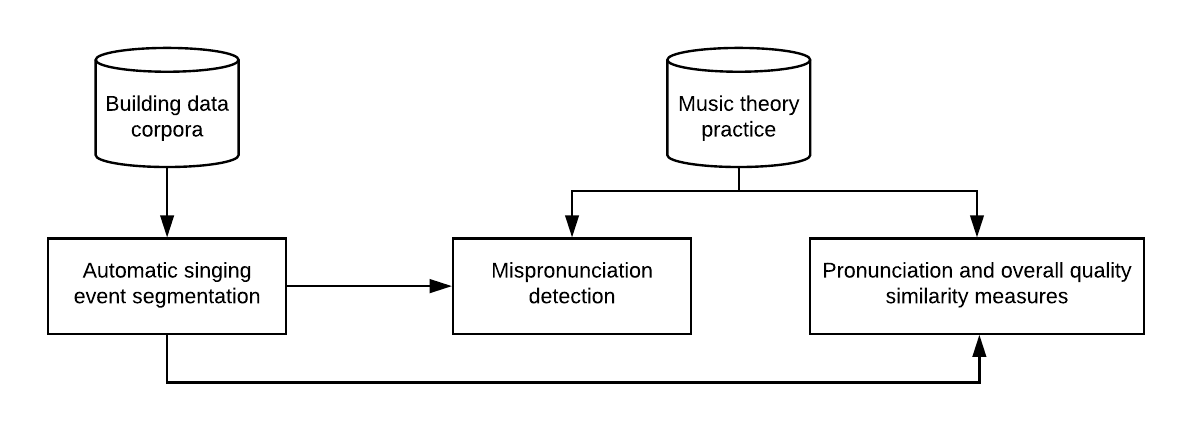
\includegraphics[width=\textwidth]{figs/blockDiags_rong/ch3_related_topics.png}
\caption{Related research topics of automatic assessment of singing voice pronunciation in jingju music.}
\label{fig:related_research_topics}
\end{figure}

In this dissertation, the assessment of singing pronunciation will be devised at syllable or phoneme level. There are several sub-problems which lead to the final goal -- to develop mispronunciation detection models and to define pronunciation similarity measure for jingju singing. In \figref{fig:related_research_topics}, we show the information flow between four topics of research problem that will be addressed in this dissertation -- building data corpora, automatic singing event segmentation, mispronunciation detection and pronunciation and overall quality similarity measures. There is a significant sequential order while addressing each problem, e.g. to achieve the assessment at syllable or phoneme level, mispronunciation detection and similarity measures benefit from the results of automatic singing event segmentation. The topics of mispronunciation detection and similarity measures use knowledge derived from music theory and practice, making them more culture-aware. Each of the topics will be discussed in detail.

\subsection{Building data corpora}

A crucial part of data-driven research using machine learning approaches requires good quality data. Data corpora of the music tradition under research are crucial for building and testing the automatic assessment models. The data should contain various sources such as audio, score, lyrics and manual annotation made for automatic assessment research.

The dataset created in the work \cite{repetto_creating_2014} is formed by a collection of commercial recordings, as well as their metadata. Another jingju music corpus gathered in the \cite{Tian2016} also consists of commercial recordings, and annotated for structural segmentation analysis. These recordings are all mixed with instrumental accompaniment, which means a cappella (clean) singing voice should be separated during the preprocessing step if we want to make use of these recordings for the research of automatic assessment. A collection of 92 jingju music scores gathered for the analysis of jingju musical system is presented in the work \cite{Repetto2017}, which is transcribed from published books and stored in machine-readable format. The a cappella singing separated commercial recording dataset and the modified score dataset will be integrated into the data corpora of this dissertation.

The a cappella jingju singing dataset created in the work \cite{black_automatic_2014} consists of 31 unique arias in total around 1-hour recordings. However, due to the small size of this dataset, and that its annotations were made for the task of mood recognition rather than automatic assessment, we have to re-annotate this dataset firstly, and then expand it to a proper scale. One of the main problems tackled in this dissertation is building suitable and scalable data corpora for the singing pronunciation assessment research, a problem that is discussed further in \secref{sec:ch3:dataset_research}. 

\subsection{Automatic singing event segmentation}

Automatic singing event segmentation includes a set of problems that aim to infer or time align the boundaries of several musical events in singing recordings related to pronunciation assessment. The common MIR tasks such as musical structure segmentation, lyrics-to-audio alignment and singing event onset detection can be classified as automatic singing event segmentation problems. As we have mentioned in \secref{sec:ch3:dataset_research}, in the context of the assessment of jingju singing pronunciation, the relevant singing events to consider are banshi, couplet, melodic line, syllable and phoneme. 

Automatic singing event segmentation is an important preliminary step to achieve automatic assessment, and there are several applications in which the segmentations are useful, such as rhythm-based annotation of audio, beat/melodic line/syllable aligned processing of music, audio summarization. Each of these problems will be described in detail.

\subsubsection{Banshi segmentation}

Banshi segmentation (or banshi tracking) is not the problem which will be tackled in this dissertation. However, we discuss it for completeness. Banshi segmentation refers to a set of problems that focus on segmenting different banshi sections in a jingju aria. By segmenting the banshi sections, a complete description of jingju metrical structure can be achieved. For such a problem, the subcomponents of a banshi -- tempo, accented beat (ban or downbeat), unaccented beat (yan or beat) can be obtained.

Banshi segmentation can be done either in an uninformed or informed fashion. The former fashion means that inferring the time-varying tempo, beats and downbeats without any prior banshi knowledge of the aria. Informed banshi segmentation is the case to track tempo, beats and downbeats given the information of the banshi sequence of the aria. We can classify the subtasks as tempo tracking, beat tracking and downbeat tracking. Tempo tracking aims to estimate the time-varying tempo over the recording of a jingju aria. The tracked tempo will be useful for the beat tracking tasks. As we have mentioned in \secref{sec:ch3:dataset_research}, the tempo tracking method applied for jingju aria needs to be robust for the local or long-term tempo change. For metered banshi, the rhythmic beats are performed by several percussion instruments -- danpigu, ban, naobo, daluo and xiaoluo. Thus, the beat time instance is defined by the onset of each percussion instrument stroke. Although a specific beat tracking algorithm has not been developed for estimating metered jingju banshi, a suitable jingju percussion onset detection method \cite{Tian2014} and several beat tracking methods \cite{Bock2011, Krebs, Bock} for eurogeneric music can be adapted for this purpose. In jingju performance, each downbeat is usually marked by the ban (wooden clapper) sound and indicates the first beat a measure \cite{Wichmann1991a}. Thus downbeat tracking can be formulated as the problem of estimating the onset time positions of the ban sound in the beat sequence. Lastly, metered banshi tracking in jingju aria is a task analogous to tala tracking in Indian art music, of which the relevant methods have been studied extensively in Srinivasamurthy's work \cite{Srinivasamurthy2016}.

Due to the lack of tempo and beat, segmenting metered banshi requires a different framework mentioned above. Banshi segmentation is an important step towards any finer segmentation task of jingju aria. However, since we adopt the melodic line directly as the input of the assessment pipeline, banshi segmentation will not be a problem considered in this dissertation.

\subsubsection{Couplet, melodic line, syllable and phoneme segmentation}

Couplet or melodic line segmentation refers to estimate the time boundaries of singing couplet or melodic line in a banshi section. The syllable or phoneme segmentation aims to transcribe the audio recording of a melodic line into a time-aligned syllable or phoneme sequence. In jingju singing training scenario, the score, lyrics and relevant annotations such as starting and ending syllables of the couplet or melodic line are usually given beforehand. Thus, these problems can be formulated into a uniformed framework -- lyrics-to-audio alignment. Time-aligning lyrics to audio is a fine-grained segmentation task, which can be applied to the syllable or phoneme level singing assessment and analysis.

Jingju is sung in Chinese Mandarin language with regional dialect pronunciations of which each written character is pronounced as a syllable (\secref{sec:ch2:jingju_syllable}), and several written characters make up a word. Although not many languages in the world adopt the similar writing system, the pronunciation of all languages is built upon basic units -- phoneme and syllable \cite{Moran2014}. Thus the lyrics-to-audio alignment method can be devised as either language-dependent or language-independent. Both methods can be formulated as supervised learning tasks. The former uses label data to build syllable or phoneme models; while the latter uses labelled data to build syllable or phoneme boundary models.

As discussed in \secref{sec:ch3:challenges}, several jingju singing characteristics such as long syllable, silences within a syllable and spectral pattern variation pose challenge to the lyrics-to-audio alignment task. Apart from that, another challenge is that the mapping from the written characters to syllables is not unique, due to the existence of special pronunciations and multi-pronunciation characters in jingju singing.

The work on lyrics-to-audio alignment for jingju singing has been very limited so far. Dzhambazov et al. \cite{dzhambazov_modeling_2015} proposed a modified text-to-speech alignment method for jingju singing. The system is built upon a duration-explicit hidden Markov model, where the phoneme duration is empirically set according to lyrics and metric structures of jingju music.

It is to be noted that prior musical information such as score is usually available for the assessment of jingju singing, and can be exploited to tackle the related challenges. Lastly, since we adopt the melodic line directly as the input of the assessment pipeline, couplet or melodic line segmentation will not be a problem considered in this dissertation. Syllable and phoneme segmentation is one of the problems addressed in this dissertation and is formulated more concretely in \secref{sec:ch3:segmentation_formulation}.

\subsection{Mispronunciation detection}\label{sec:ch3:mispronunciation_challenge}

Mispronunciation detection refers to build the computational model to detect the badly pronounced syllables or phonemes in student's singing voice. The detection could be done in either syllable or phoneme granularities. In this dissertation, we tackle only the problem of building the models to detect the mispronunciation at syllable-level since syllable or written-character is the basic unit of which the teacher corrects the pronunciation in the actual singing training scenario. More specifically, we tackle only the problem of mispronunciation detection for jiantuanzi and special pronounced syllables since these two types of the syllable is the main source of the mispronunciation in jingju singing training. The application of such detection model is not limited to singing voice. Other potential applications are the mispronunciation detection in the second language (L2) learning or broadcasting training.

The challenge of this topic, as mentioned in \secref{sec:ch3:challenges}, is to take consideration of the locality of the mispronunciation within a syllable, which is to say, the model should be able to detect the mispronunciation of a syllable according to some parts of the syllable. We can formulate the detection problem as a supervised discriminate task, and a labeled dataset which contains mispronunciation syllable segments (positive samples) and correctly pronounced syllable segments (negative samples) can be used to build the model.

There exist a significant amount of works on the topic of speech mispronunciation detection applied in L2 learning. The most relevant work in this field is the Goodness of pronunciation (GOP) measure proposed by S. M. Witt and S. J. Young \cite{Witt2000}, which used forced alignment method with a pronunciation dictionary to generate GOP score for the mispronunciation detection task of English phonemes. In the singing voice application, Gupta et al. \cite{Guptac} first generalized the mispronunciation rules for the singing voice of Southeast Asian English accent. Then they also applied forced alignment with an adapted dictionary for the mispronunciation detection.

Mispronunciation detection is one of the problems addressed in this dissertation. A more comprehensive problem formulation will be presented in \secref{sec:ch3:mispronunciation}.

\subsection{Pronunciation and overall quality similarity measures}

Pronunciation and overall quality similarity measures refer to build an objective model to calculate the similarity of corresponding jingju singing segments between teacher and student respecting pronunciation and overall quality aspects. The similarities can be measured in different singing granularities such as banshi section, couplet, melodic line, syllable and phoneme. In this dissertation, we tackle only the problem of building the models of phoneme-level pronunciation and overall quality similarity measures since phoneme is the finest grained pronunciation unit of jingju singing, and the composition basis of any higher singing granularities such as syllable, melodic line, couplet and banshi section. Likewise, phoneme is also the finest grained pronunciation unit of any other languages. The method developed in building similarity measures at phoneme-level in jingju singing can be easily adapted to singing similarity measurement at phoneme-level in any other languages. The application of such similarity measure is not limited to the assessment of singing voice. Other potential applications are the assessment of pronunciation at phoneme-level in the second language (L2) learning and broadcasting training. In such scenarios, the similarity between the phoneme segments of a language learner and a native speaker needs to be shown to give the learner a clue about how well her/his pronunciation or overall quality is. 

The challenge of this topic, as mentioned in \secref{sec:ch3:challenges}, is to find proper representations for similarity measures -- representation learning. Pronunciation is represented in the signal point of view as the time-varying spectral change. Overall quality is a perceptual concept mixed with different musical dimensions such as intonation, loudness, duration and timbre. The representations need to capture the time-varying and abstractive natures of these two concepts. The representation learning can be formulated as a supervised discriminative or a semi-supervised distance metric learning tasks. Take overall quality aspect as an example, a supervised discriminative learning uses labeled data (e.g. good/bad quality) to build a discriminative model, while a semi-supervised distance metric learning uses data labeled in pairwise or triple-wise similarity to build a model, e.g. the overall quality of samples A and B are similar; that of sample B and C are not similar. As a consequence, the learned representation from either the discriminative model or distance metric learning model is used for the similarity measurement.

We cannot identify any previous work on the topic of pronunciation or overall quality similarity measure at phoneme-level. However, there exist a significant amount of works on the topic of speech phonetic similarity applied in L2 learning. Minematsu et al. \cite{Minematsu2004, Minematsu2007, Shiozawa2016} propose a structural representation of speech phoneme sounds. They train HMM for each phoneme class, then compute Bhattacharyya distance between each HMM pairs. The pairwise distance matrix represents the phoneme-level linguistic structure. They also claim that this representation is represent purely the linguistic traits of a language and free from any distortion such as microphone, room, speaker. Thomson \cite{Thomson2008} develops a method to measure the English vowel similarity for Mandarin speaker. He builds discriminative models for each English vowel using the recordings of English native speakers, then uses the models to calculate the posterior probability as the similarity measure for vowel segment of Mandarin speakers. Wieling et al. \cite{Wieling2011} focus on the multidimensional scaling (MDS) representation of vowel segments. They use formant frequencies as the feature to calculate the euclidean distance for each vowel pair, then perform MDS to project each vowel onto a two-dimensional similarity space. Mielke \cite{Mielke2012} explores DTW distance for phonetic similarity measure. He uses MFCC as the representation of the phoneme segment, and compute DTW distance between two MFCC vectors. Kyriakopoulos et al. \cite{Kyriakopoulos2017} develop a phoneme similarity measure based on Jensen-Shannon divergence. They calculate aggregate PLP feature and fit multivariate Gaussian model for each phoneme. The Jensen-Shannon distance is computed on the multivariate Gaussian models of each phoneme pair.

Pronunciation and overall quality similarity measures are one of the problems addressed in this dissertation. A more comprehensive problem formulation will be presented in \secref{sec:ch3:similarity_formulation}.

\section{Formulation of thesis problems}

With an overview of the research problems, challenges, review of the state of the art works, a subset of those problems that will be tackled in this dissertation are defined. In this section, we formulate these problems more comprehensively by discussing their assumptions, restrictions, and objectives in an engineering way.

\subsection{Dataset for research}\label{sec:ch3:dataset_research}

Building a dataset for MIR research is a scientific problem. Objective criteria are set up for designing, curating and also measuring the goodness of a corpus. One of the goals of CompMusic project is to build such data corpora and make it available for the research usage. Collection of good quality data and easily accessible audio and metadata is crucial for the research reproducibility.

For developing relevant approaches, we focus on collecting and curating a cappella (clean) jingju singing voice audio in jingju singing training scenario. The jingju a cappella audio dataset includes both professional (teacher) singing audio and amateur (student) imitative singing audio, which accompanied with hierarchical jingju musical events annotations. For all of the tasks addressed in this dissertation, we need singing syllable and phoneme boundary annotations. Specifically, for mispronunciation detection task, we annotate special pronunciation singing syllables. 

In general, for the research of automatic assessment of jingju singing voice, we aim to build a data collection which can represent the real world singing training scenarios. The recordings need to include the main role-types disciplined in singing, common teaching repertoire. The datasets built in the context of this dissertation are further presented in Chapter 4.

\subsection{Syllable and phoneme segmentation}\label{sec:ch3:segmentation_formulation}

One of the problems addressed in this thesis is syllable and phoneme segmentation of jingju singing recordings. To the best of our knowledge, for jingju music, a system which can achieve a certain segmentation accuracy to be suitable for the needs of automatic assessment at syllable or phoneme level does not exist yet. Additionally, to improve the segmentation accuracy, we also explore incorporating a priori musical information such as the syllable or phoneme duration extracted from music scores or annotations into the segmentation algorithm.

To address the problem, we formulate tasks that can integrate a priori syllable or phoneme duration information -- duration-informed syllable and phoneme segmentation. The a priori duration information is extracted either from the musical score or manual annotation, which thus represents the coarse syllable or phoneme duration in the target recording. We then use data-derived audio representation indicative of syllable or phoneme onset events in the recording. Finally, we build hidden Markov models that can incorporate the a priori duration information into the syllable or phoneme boundary selection step. The onset detection-based rather than the forced alignment-based approach is used since the former is a binary classification task which requires less training data, and onset time stamps annotation is available for model training.

In the scope of this work, the target singing recording is assumed to have been already segmented into pieces that are in a single melodic line. This assumption mainly stems from the fact that in the actual jingju singing training course, the materials are taught and practised line by line. We do not assume any restrictions on banshi type over the melodic line. We restrict our work to two role-types -- dan and laosheng in jingju music. The restriction is mainly because dan and laosheng are respectively two major role-types of female and male singing styles, and that singing is the main discipline of these two role-types. The proposed method is likely to extend to the singing of other role-types, provided we have the a priori duration information for them. 

The a priori syllable durations of the target melodic line are stored in an array $M^s=\mu^{1} \cdots \mu^{n} \cdots \mu^{N}$, where $\mu^{n}$ is the duration of the nth syllable. The a priori phoneme durations are stored in a nested array $M_p=M^{1}_p \cdots M^{n}_p \cdots M^{N}_p$, where $M^{n}_p$ is the sub-array with respect to the nth syllable and can be further expanded to $M^{n}_p=\mu_{1}^{n} \cdots \mu_{k}^{n} \cdots \mu_{K_{n}}^{n}$, where $K_{n}$ is the number of phonemes contained in the nth syllable. The phoneme durations of the nth syllable sum to its syllable duration: $\mu^{n}=\sum_{k=1}^{K_{n}} \mu_k^{n}$. In both syllable and phoneme duration sequences -- $M^s$, $M_p$, the duration of the silence is not treated separately and is merged with its previous syllable or phoneme. Let the recording of a melodic line can be reduced by short-term Fourier transform (STFT). The goal is to find the best onset state sequence $Q={q_1 q_2 \cdots q_{N-1}}$ for a given syllable duration sequence $M^s$ or phoneme duration sequence $M_p$ and impose the corresponding syllable or phoneme label, where $q_i$ denotes the onset of the $i+1$th or the offset of the $i$th inferred syllable/phoneme.

The approaches, experiments and results for syllable and phoneme segmentation are presented in Chapter.

\subsection{Mispronunciation detection}\label{sec:ch3:mispronunciation}

The problem of mispronunciation detection at syllable-level is the third problem that will be addressed in this thesis. The goal is to build supervised discriminative deep learning models to classify mispronounced and correctly pronounced syllabic segments. We explore integrating the attention mechanism into the approach, and the learned model is supposed to concentrate on some certain parts of the syllable. Differ from the widely adopted forced alignment-based approach, the proposed method only requires that the training data has the binary annotation -- mispronounced or correctly pronounced, rather than the detailed mispronunciation patterns.

As the preliminary step, the syllables are segmented automatically by using the approach presented in \secref{sec:ch3:segmentation_formulation}. Although this approach will cause some segmentation errors which might be propagated to the mispronunciation detection step, we use it to allow a fair comparison with the baseline forced alignment-based method, since the latter also segment the syllables automatically. We restrict in this dissertation the mispronunciation detection on two types of the syllable -- jiantuanzi and special pronunciation since they are the main sources of mispronunciation happened in actual jingju singing training. Jiantuanzi mispronunciation means that the student mispronounces a pointed sound syllable (jianzi) as the rounded sound (tuanzi). The mispronunciation of the special syllables means that the student mispronounces a special pronounced syllable as the standard pronunciation in Chinese Mandarin. The mispronunciation patterns -- from correctly pronounced syllable to mispronounced syllable, is shown in \appref{app:special_pronunciation}. Thus, two different models will be explored. The first one classifies the mispronounced special syllables from the correctly pronounced special syllables, and the second one classifies the mispronounced jianzi from the correctly pronounced jianzi.

Let the set of variable-length mispronounced special syllable segments be denoted as $S_{positive}$, and the set of correctly pronounced special syllable segments to be denoted as $S_{negative}$. The discriminative model should be able to classify binarily the samples between these two classes. The similar model can be built for jiantuanzi mispronunciation detection as well. 

The approaches, experiments and results for mispronunciation detection are presented in chapter.

\subsection{Pronunciation and overall quality similarity measures at phoneme level}\label{sec:ch3:similarity_formulation}

The problem of pronunciation and overall quality similarity measures is the fourth problem that will be addressed in this thesis. The approach we explore is to learn phonetic pronunciation and overall quality representations using representation learning techniques and compute the similarity between two representations using distance measure. The goal is to test the effectiveness of representation learning techniques in learning pronunciation or overall quality discriminative representations. Differ from the previous similarity measure approaches which use handcrafted features as the representation, and perform DTW related methods to compute the similarity between two variable-length features, we present an approach in this dissertation based on acoustic phoneme embeddings which map the variable-length phoneme segments into fixed-length vectors, which facilitate the similarity calculation.

We assume that the singing recordings have been segmented into phoneme units, which is done manually in this dissertation. Although the segmentation can be done automatically by using the approach presented in \secref{sec:ch3:segmentation_formulation}, this assumption can make sure the segmentation accuracy, and thus avoid the error propagated by the automatic segmentation step. We restrict in our work the overall quality to be a binary rubric such that phoneme segments sung by the teacher have a professional overall quality, and those sung by the student have an amateur overall quality. Thus, the overall quality similarity is measured between teacher and student phoneme segment pair which belong to the same phoneme class. For example, the approach can only measure the similarity between phoneme segments A and B, where A is sung by teacher and B is sung by student; A, B belong to the same phoneme class. From the point of view actual jingju singing training, only the case mentioned above is valid since the similarity between two phoneme segments sung consistently by teacher or student would not be measured, and measuring the similarity between two segments belonging to different phoneme classes is a problem which can be avoided by mispronunciation detection. Since we can be sure that the student recordings in our dataset can by no means reach the professional level, such a restriction is justified.

Let the set of variable-length phoneme segments be denoted as $\mathcal{A} = {A_1, A_2, A_3, ..., A_N}$, where each $A_j$ is a subset of phoneme segments belonging to class j. The learned phonetic pronunciation representation for each phoneme segment in $A_j$ should be capable of minimizing the intra-class similarity and maximizing the inter-class similarity. Let the set of variable-length phoneme segments sung by teacher be denoted as $\mathcal{B}={B_1, B_2, B_3, ..., B_{N}}$, and another set of variable-length phoneme segments sung by student be denoted as $\mathcal{C}={C_1, C_2, C_3, ..., C_{N}}$, where each $B_j$ and $C_j$ are the subsets of phoneme segments belonging to class j. The learned phonetic overall quality representation should be capable of minimizing the intra-class similarity between two segments from one single set such as B or C, and maximizing the inter-class similarity between those from different sets such as $B_j$ and $C_j$. 

The whole approach can be formulated as a fixed-length representation learning problem with pre-segmented phoneme samples -- using the fixed-length representation for the similarity computation. The approaches, experiments and results for syllable and phoneme segmentation are presented in Chapter.
\chapter{Data corpora for research}\label{chap:datasets}
% \begin{epigraphs}
%   \qitem{Data is a precious thing and will last longer than the systems themselves.}{Tim Berners-Lee}% , inventor of the World Wide Web
% \end{epigraphs}
% Use \noindent for the first paragraph after this
%\dtext{The work we do is data-driven and hence datasets play an important role in research. A significant part of the efforts in the CompMusic project and the thesis are to collaborate and develop datasets for use in research. The chapter discusses the datasets developed within the context of CompMusic, by us and other collaborators. The idea is also to discuss how to measure the goodness of a corpus, what data driven research can be done with datasets and what can we learn directly from datasets.}
%
%\dtext{Abstract: Research corpora are representative collections of data and are essential to develop data-driven approaches in Music Information Research (MIR). We address the problem of building research corpora for MIR in Indian art music traditions of Hindustani and Carnatic music, considering several relevant criteria for building such corpora. We also discuss a methodology to assess the corpora based on these criteria and present an evaluation of the corpora in their coverage and completeness. In addition to the corpora, we briefly describe the test datasets that we have built for use in many research tasks. In specific, we describe the tonic dataset, the Carnatic rhythm dataset, the Carnatic \gls{varnam} dataset, and the Mridangam stroke dataset.}

Computational data-driven MIR research requires a well-curated data corpus for training and testing the models. The corpus should meet certain criteria so that the models can be built successfully built and applicable to real-world scenarios. A research corpus is an evolving data collection which is representative of the research domain under study. A good corpus can be built by a single research institute or by crowdsourcing within a community. Regarding MIR research, a research corpus is a representative subset of one or several music genres, since it is nearly impossible to work with all the relevant music pieces. Computational models developed upon this subset can be assumed generalizable to real-world scenarios.

A test dataset is a subset of the research corpus which is designed for a specific research task. In the research task, the test dataset is used to develop and evaluate computational models. For better reproducibility of experiment results, the test dataset is usually fixed or properly versioned.

Building a research corpus is a research problem itself and has been studied in many fields. There are many repositories for the research of speech such as Linguistic Data Consortium\footnote{\url{https://www.ldc.upenn.edu/}}, Librispeech\footnote{\url{http://www.openslr.org/}}, and for the research of musicology such as IMSLP/Petrucci Music Library\footnote{\url{https://imslp.org/}} and MusicBrainz\footnote{\url{https://musicbrainz.org/}}. There have been efforts to compile large collections for MIR or general sound analysis research such as Million Song Dataset \cite{Bertin-Mahieux2011a}, FMA dataset \cite{Defferrard2017}, AcousticBrainz\footnote{\url{https://acousticbrainz.org/}} and Freesound datasets \cite{Fonseca2017}. These music data collections are good resources for developing MIR models on Western Pop music. A systematic way of building a research corpus is essential for the MIR research, and receives attention from the research community. Serra \cite{Serra2014} described a set of criteria to build a MIR research corpus -- Purpose, Coverage, Completeness, Quality and Reusability. We use these criteria to help develop a corpus for automatic assessment of jingju singing pronunciation.

In this chapter, we compile and analyse the research corpus and test datasets for the research of this dissertation. We will discuss the corpus building criteria and evaluation methodologies. Our main focus in this chapter will be jingju music, while other relevant test datasets are also presented. We aim:

\begin{enumerate}[noitemsep]
\item To describe the corpus and the test datasets, emphasizing the research problems and tasks relevant to this thesis.
\item To describe a set of corpus design criteria and methodologies, then use them to evaluate the jingju a cappella singing voice corpus.
\item To present both corpus-level and test dataset-level musically meaning data analysis and visualization.
\end{enumerate}

We mainly emphasize on presenting a scientific approach for corpus building and the evaluation of its coverage and completeness. Apart from the corpus description, the musically meaningful data analysis and visualization is another contribution of this chapter. Finally, the research corpus and test datasets presented in this chapter will be made available for further jingju MIR research.

\section{CompMusic research corpora}\label{sec:ch4:compmusic_corpora}

Although different music genres share some basic concepts such as melody and rhythm, some other important aspects can be described only by considering the musical specificity of that tradition. In the context of CompMusic project, Serra \cite{serra_multicultural_2011} highlighted the needs for culture-specific MIR research corpora to develop approaches which benefit from the essential aspects of the music tradition. 

In CompMusic project, we work with five music traditions of the world which expose different research problems. A significant effort has been put towards the design the research corpora for the relevant problems of the specific musical traditions. In this chapter, we focus mainly on the a cappella singing voice of jingju music, while jingju commercial audio recording \cite{repetto_creating_2014}, lyrics and musical score collections \cite{Repetto2017} have been presented by other researchers of the CompMusic project. The Carnatic and Hindustani research corpora have been described thoroughly by \cite{Srinivasamurthy2014}. The Turkish makam music research corpus has been presented in detail by \cite{Uyar2014a}.

\subsection{Criteria for the creation of research corpora}

Serra \cite{Serra2014} listed five criteria for build culture-specific MIR research corpus:

``Purpose: The first step in the design of a corpus is to define the research problem that wants to be addressed and the research approach that will be used. In CompMusic, we want to develop methodologies with which to extract musically meaningful representations from audio music recordings, mainly related to melody, rhythm, timbre and pronunciation. The approaches are based on signal processing and machine learning techniques; thus the corpus has to be aligned with this purpose.

Coverage: A corpus has to include data representative of all the concepts to be studied and given our quantitative approach, there have to be enough samples of each instance for the data to be statistically significant. For our research we need to have audio recordings, plus appropriate accompanying information, covering the varieties of pronunciation present in the musical culture.

Completeness: In each corpus, every audio recording is complemented by a set of data fields, and the idea of completeness relates to the percentage of fields filled, thus how complete the corpus is. For our corpora, this mainly refers to the completeness of the editorial metadata and the annotations accompanying each audio recording.

Quality: The data has to be of good quality. The audio has to be well recorded and the accompanying information has to be accurate. We have used well-produced recordings whenever possible, and the accompanying information has been obtained from reliable sources and validated by experts.

Reusability: The research results have to be reproducible, and that means that the corpus has to be available for the research community to use. In our case, we have emphasised the use of specific open repositories such as Zenodo.org\footnote{\url{https://zenodo.org/}} that are either already suitable or that can be adapted to our needs."

Central to the jingju a cappella singing corpus is the audio recordings with its annotation. We present this corpus in the next section.

\subsection{Jingju a cappella singing corpus}\label{sec:ch4:jingju_acappella_singing_corpus}

The jingju a cappella singing corpus mainly contains audio recordings, editorial metadata and musical event annotations. All annotated corpus is the content used by signal processing and machine learning approaches.

Given that aria is the natural unit of jingju music, most audio recordings in this corpus are arias. A unique aria might be sung by different singers with different singing levels -- professional or amateur. To facilitate the development of singing voice assessment models, the audio recordings in this corpus are all a cappella version, meaning without instrumental accompaniment. The singer's singing level is most important metadata associated with a recording.

To build the corpus, we consulted jingju professors and musicologists. The main institutional reference is the National Academy of Chinese Theatre Arts (NACTA)\footnote{\url{https://www.nacta.edu.cn/}}, which is the premier institution dedicated to jingju performing training in Beijing, China, and is the only institute of its kind in China that offers both B.A. and M.A. degrees in jingju performing.

We wish to compile recordings sung by both professional and amateur singers from different backgrounds. The professional recording singers are the professors and students of NACTA. The amateur singers are from various sources -- students of jingju associations in non-art universities, amateurs of jingju groups in community activity centers located in Beijing, amateurs of jingju associations located in London and students from several primary schools. We did not keep track the singer information of the amateurs of jingju groups in community activity centers located in Beijing and the students from several primary schools due to that a large number of singers participated in these recording sessions. Otherwise, the singer information of the other recordings is written in the editorial metadata. 

The corpus has been collected in three different stages and thus been split into three parts. The audios in the first part are recorded with the joint effort of two music technology research institutes -- Center for Digital Music, Queen Mary University of London (C4DM) \cite{Black2014} and Music Technology Group, Universitat Pompeu Fabra (MTG-UPF). Additionally, another 15 clean singing recordings separated from the commercial releases have been included in this part. The audios in the second and third parts are recorded by the author of this thesis during his two times research stay in Beijing.

The corpus consists of 2 role-types (dan and laosheng), 121 unique arias with 289 recordings, meaning several arias have been recorded more than once by different singers. The total duration is 13.61 hours. Other information related to the corpus is described in \tabref{table:ch4:general_statistics_jingju_a_cappella_corpus}.

\begin{landscape}
\mbox{}\vfill
\begin{table}[ht]
    \centering
    \begin{tabular}{l|ccccc}
        \toprule
        Role-type & \makecell{\#Unique aria\\(A: amateur,\\P: professional)} & \#Recording & \#Singers & \makecell{\#Total duration\\(hours)} & \makecell{\#Median recording\\duration (minutes)} \\
        \midrule
        dan           & 73 & 171 (A: 79, P: 83) & 14+ & 8.26 & 1.87 \\
        laosheng      & 48 & 118 (A: 67, P: 51) & 13+ & 5.35 & 2.01 \\
        \bottomrule
    \end{tabular}
    \caption{General statistics of the jingju a cappella singing corpus}
    \label{table:ch4:general_statistics_jingju_a_cappella_corpus}
\end{table}
\vfill
\end{landscape}

The editorial metadata associated with each recording has been stored in MusicBrainz, as well as in Zenodo.org. The primary metadata is the name of the aria, the name of the play and the name of the singers. Each entity such as artist, recording, work, in MusicBrainz is assigned a unique MusicBrainz IDentifier (MBID), which helps organize the metadata. The editorial metadata has been entered using simplified Chinese characters and romanization system -- pinyin. 

A large part of the audio recordings has been annotated. The annotations consist of (i) melodic line onset and offset time boundaries and lyrics in simplified Chinese characters, (ii) syllable onset time stamps and pinyin label, (iii) phoneme onset and offset time boundaries and X-SAMPA label (\appref{app:mandarin_sounds}), (iv) labels indicating the melodic lines which contain long syllables and (v) labels indicating special pronunciations. All annotations have been done in Praat speech analysis and annotation tool \cite{boersma_praat_2001}. Two Mandarin native speakers and one jingju musicologist have dedicated to the annotation. The annotation has been verified and corrected twice by the thesis author to ensure its the boundary accuracy and label correctness.

The whole corpus including audio recordings, editorial metadata and audio annotations are easily accessible from Zenodo.org\footnote{\url{https://doi.org/10.5281/zenodo.780559}}\footnote{\url{https://doi.org/10.5281/zenodo.842229}}\footnote{\url{https://doi.org/10.5281/zenodo.1244732}}.

\subsubsection{Recording setup}\label{sec:ch4:recording_setup}

In the first part of the corpus, the information of recording setup for the audios collected by C4DM has not been given in the original release \cite{Black2014}. However, by listening to each of them, we confirmed that the audios from this part included in the corpus are all good quality. Also in this part, the recordings whose names ending with `upf' are recorded in a professional studio with jinghu accompaniment. Singers and jinghu accompanists are placed separately in different recording rooms and used two recording channels to avoid crosstalk. Other recordings whose name ending with `lon' are recorded by using a Sony PCM-50 portable stereo recorder in a classroom with a certain reverberation. Additionally, another collection of 15 clean singings source-separated from commercial recordings contain audible artefacts of the background accompaniment.

For the second part of the corpus, most of the recording sessions have been conducted in professional recording rooms by using professional equipment. We use two recording equipment sets and two recording rooms:

\begin{itemize}[noitemsep]
    \item Set 1: M-Audio Luna condenser microphone + RME Fireface UCX audio interface + Apple GarageBand for Mac DAW;
    \item Set 2: Mojave MA-200 condenser microphone + ART voice channel microphone preamp + RME Fireface 800 audio interface + Adobe Audition 2.0 DAW;
    \item Room 1: The conference room in NACTA's business incubator with reflective walls, carpet-covered floor, conference furniture and medium room reverberation;
    \item Room 2: The sound recording studio in Institute of Automation, Chinese Academy of Science, with acoustic absorption and isolation.
\end{itemize}

Commercial audio recordings are used, or jingju players are invited for accompanying the singing. When commercial audio recordings were used as the accompaniment, singers were recorded while listening to the accompaniment sent through their monitoring headphone. Otherwise, when \textit{jinghu} players were used as the accompaniment, to simultaneously record both singing and \textit{jinghu} without crosstalk, we placed them separately in two different recording rooms and used two recording channels. However, they were still able to have visual communication through a window and monitor each other through headphones.

For the third part of the corpus, the recording sessions are done by using a Sony PCM-50 portable stereo recorder. The professional singings are recorded during the primary school jingju courses. The recording sessions of primary school students are done in three classrooms rather than asking the students to come to the studio. We believe that recording in the classrooms can represent the room acoustic conditions of the actual jingju teaching. The three rooms are (i) a mid-reflected classroom with the hard wall, marble floor, wood tables, chairs and a blackboard; (ii) a high-reflected dancing rehearsal room with mirrors, hard wall and wood floor; (iii) a mid-reflected dancing rehearsal room with carpet floor, mirrors and glass windows. Lastly, the amateurs of jingju groups in community activity centers are recorded in (iv) a high-reflected community entertainment room with marble floor and hard wall.

\subsubsection{Coverage}

A research corpus needs to be representative of the real world in the concepts that are primary to the music culture \cite{Srinivasamurthy2016}. The main concepts of jingju music -- role-type, shengqiang and banshi, are presented previously in \secref{sec:ch2:jingju_music}. The concepts of jingju singing -- syllable and phoneme are the essential units for the pronunciation assessment. In this work, the coverage analysis is presented for role-type, shengqiang, banshi and phoneme. We do not analyse syllable because there are excessive syllable classes in the languages of jingju singing.

The corpus includes the two jingju role-types whose main discipline is singing -- \textit{laosheng} and \textit{dan}. Both professional and amateur singers have been recorded. For \textit{dan} role-type, there are 79 amateur recordings and 83 professional recordings. For \textit{laosheng} role-type, there are 67 amateur recordings and 51 professional recordings (see \tabref{table:ch4:general_statistics_jingju_a_cappella_corpus}).

\begin{table}[ht]
    \centering
    \begin{tabular}{l|cc}
        \toprule
        Role-type & shengqiang & banshi \\
        \midrule
        dan           & \makecell{xipi, erhuang,\\fanxipi, fanerhuang,\\nanbangzi, sipingdiao,\\fansipingdiao, gaobozi,\\handiao} & \makecell{yuanban, manban,\\kuaiban, liushui,\\erliu, kuaisanyan,\\sanyan, pengban,\\shuban, duoban,\\daoban, huilong,\\yaoban, sanban} \\
	    \hline
	    laosheng      & \makecell{xipi, erhuang,\\fanxipi, fanerhuang} & \makecell{yuanban, manban,\\kuaiban, liushui,\\erliu, kuaisanyan,\\zhongsanyan, sanyan,\\daoban, huilong,\\yaoban, sanban} \\
        \bottomrule
    \end{tabular}
    \caption{A list of shengqiang and banshi included in the corpus.}
    \label{table:ch4:shengqiang_banshi_corpus}
\end{table}

The corpus also includes the two main \textit{shengqiang} - \textit{xipi} and \textit{erhuang}, and a few auxiliary ones, such as \textit{fanxipi}, \textit{fanerhuang}, \textit{sipingdiao}, \textit{nanbangzi}.

In terms of \textit{banshi}, the whole range of metered ones is represented in the dataset - \textit{yuanban}, \textit{manban}, \textit{kuaiban}, \textit{erliu}, \textit{liushui}, \textit{sanyan} and its three variations -- \textit{kuaisanyan}, \textit{zhongsanyan} and \textit{mansanyan}. Besides these metered \textit{banshi}, there are a few unmetered ones -- \textit{sanban}, \textit{daoban}, \textit{yaoban} and \textit{huilong}, whose occurrence is very punctual in performance. A list of shengqiang and banshi included in the corpus for \textit{dan} and \textit{laosheng} role-types is shown in \tabref{table:ch4:shengqiang_banshi_corpus}.

\begin{figure}[ht!]
    \centering
    \subfloat[Dan role-type]{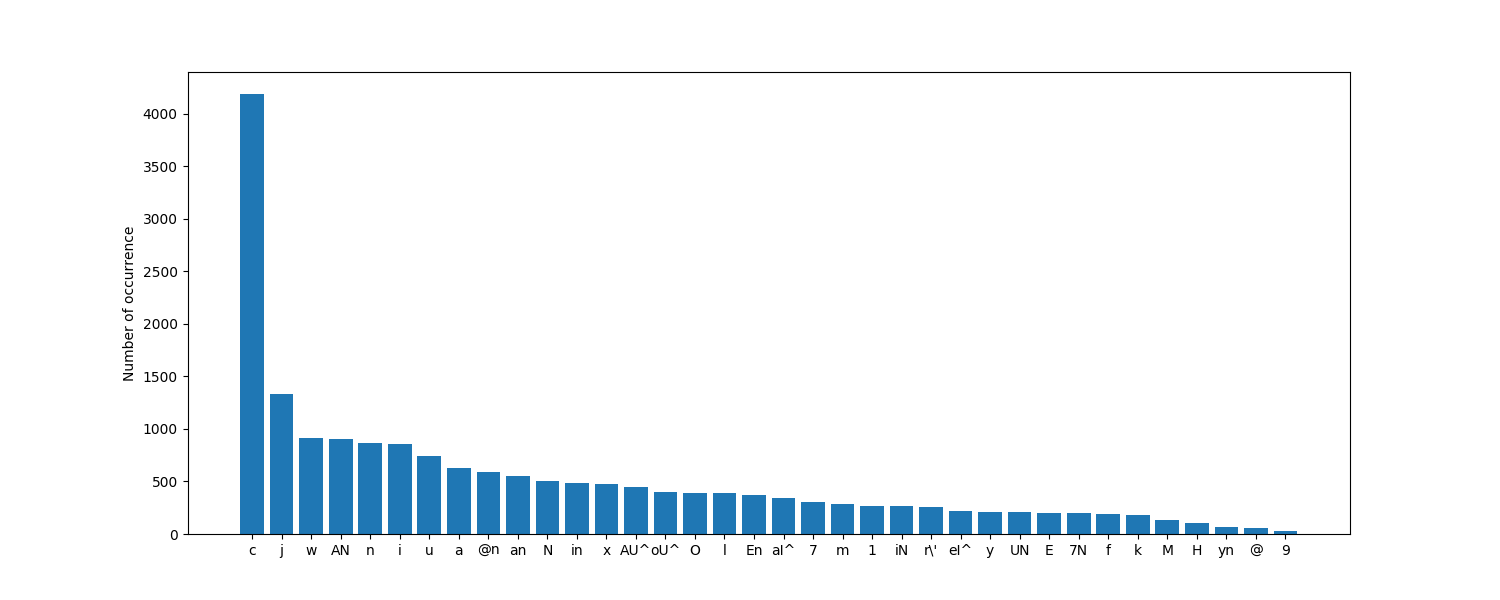
\includegraphics[width=\textwidth]{figs/dstats/dan-number-occurrence.png}
        \label{fig:ch4:number_occurrence_dan}}
    \hfill
    \subfloat[Laosheng role-type]{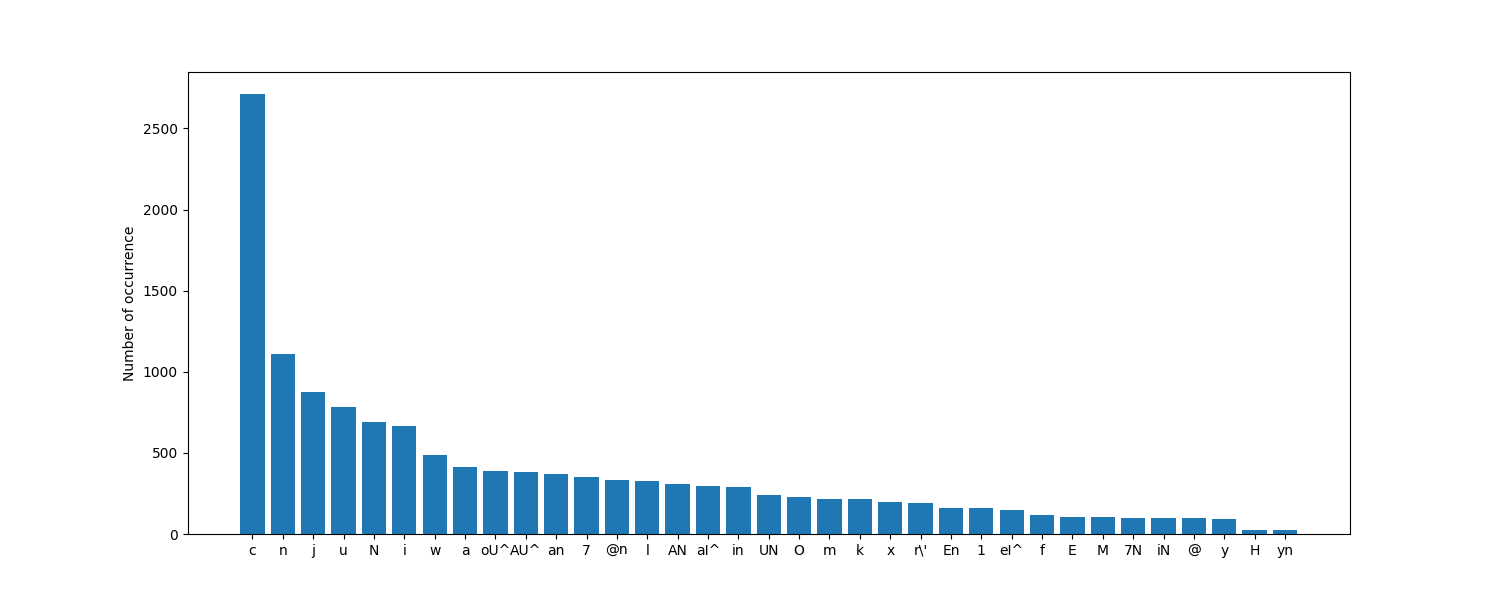
\includegraphics[width=\textwidth]{figs/dstats/laosheng-number-occurrence.png}
        \label{fig:ch4:number_occurrence_laosheng}}
  
    \caption[]{Number of occurrence for each phoneme of dan and laosheng role-types.}
    \label{fig:ch4:number_occurrence}
\end{figure}

\figref{fig:ch4:number_occurrence} represents the number of occurrence for each phoneme for dan and laosheng role-types. We can see that the corpus cover all the phoneme classes for both dan and laosheng role-types, although some phonemes such as ``@", ``yn" have tiny number of occurrence. In all the phoneme classes, ``c", a meta-phoneme class which is merged by all the non-voiced consonants, has the largest number of occurrence. An interesting observation is that the semivowel ``j" has a large number of occurrence because this semivowel is used for both syllable initial and medial vowel. Another large number of occurrence phoneme ``n" is also used for both syllable initial and terminal consonants. Phoneme ``AN" is presented much more in dan singing than in laosheng singing, which indicates that it is preferable to use the syllables constituted with this nasal final in dan singing than in laosheng singing.

\subsubsection{Completeness}

In the context of this dissertation, completeness of the corpus refers to the completeness of the associated metadata and annotation for each recording. As the metadata and annotations are important for training and testing singing assessment machine learning models, they should as complete as possible. 

\begin{table}[ht]
    \centering
    \begin{tabular}{l|cccc}
        \toprule
        Role-type & Metadata & Melodic line & Syllable & Phoneme \\
        \midrule
        dan           & 100\% & \makecell{118/171;\\69\%} 	& \makecell{110/171;\\64.32\%} 	& \makecell{92/171;\\53.8\%} \\
        \hline
        laosheng      & 100\% & \makecell{89/118;\\75.42\%} & \makecell{89/118;\\75.42\%} 	& \makecell{52/118;\\44.06\%} \\
        \bottomrule
    \end{tabular}
    \caption{Metadata and annotations completeness. Table cell format: \#annotated recordings/total recordings; percentage.}
    \label{table:ch4:metadata_completeness}
\end{table}

\begin{table}[ht]
    \centering
    \begin{tabular}{l|cccc}
        \toprule
        Role-type & \#Melodic line & \#Syllable & \#Phoneme \\
        \midrule
        dan           & 1213 	& 9847 	& 18671  	\\
        laosheng      & 893 	& 8239 	& 13378 	\\
        \bottomrule
    \end{tabular}
    \caption{The number of annotated melodic line, syllable and phoneme in the corpus.}
    \label{table:ch4:annotated_number}
\end{table}

The corpus contains the metadata of each recording -- the artist's singing level, the name of the aria, the name of the play and the name of the singing characters. The metadata is 100\% annotated for all recording in the corpus.

The annotations are done in a hierarchical way at melodic line, syllable and phoneme levels. Due to time limits, not all recordings have been annotated. The annotation completeness for each recording in different granularities is shown in \tabref{table:ch4:metadata_completeness}. The number of annotated melodic line, syllable and phoneme are shown in \tabref{table:ch4:annotated_number}.

An important concern in computational research is the reproducibility of the experiments, which requires a corpus openly accessible to the research community. All three parts of the corpus which includes audio, metadata and annotations are stored in Zenodo.org\footnote{\url{https://doi.org/10.5281/zenodo.780559}}\footnote{\url{https://doi.org/10.5281/zenodo.842229}}\footnote{\url{https://doi.org/10.5281/zenodo.1244732}}. The metadata is also organized into releases in MusicBrainz\footnote{\url{https://musicbrainz.org/search?query=jingju\&type=release\&method=indexed}}.

\subsubsection{Dataset analysis}\label{sec:ch4:dataset_analysis}

In this section, we present a corpus-level statistic analysis towards the durations of the melodic line, syllable and phoneme. The goal is to draw musically meaningful insights from the analyses. 

\begin{table}[ht]
    \centering
    \begin{tabular}{l|cc|cc|cc}
        \toprule
        \multirow{2}{*}{Role-type} & \multicolumn{2}{c|}{Melodic line} & \multicolumn{2}{c|}{Syllable} & \multicolumn{2}{c}{Phoneme} \\
        & \makecell{Mean\\Std} & \makecell{Min\\Max} & \makecell{Mean\\Std} & \makecell{Min\\Max} & \makecell{Mean\\Std} & \makecell{Min\\Max} \\
        \midrule
        dan           & \makecell{11.93\\13.85} & \makecell{1.81\\119.69} & \makecell{1.35\\2.66} & \makecell{0.07\\52.66} & \makecell{0.42\\0.75} & \makecell{0.0047\\11.08} \\
        \hline
        laosheng      & \makecell{10.02\\8.86} & \makecell{1.82\\55.92} & \makecell{1.08\\0.84} & \makecell{0.07\\20.63} & \makecell{0.29\\0.62} & \makecell{0.0025\\13.59} \\
        \bottomrule
    \end{tabular}
    \caption{Mean and standard deviation duration, minimum and maximum duration of melodic line, syllable and phoneme (second).}
    \label{table:ch4:mean_std_min_max}
\end{table}

\tabref{table:ch4:mean_std_min_max} shows a basic statistics of duration for melodic line, syllable and phoneme. Some interesting insights can be drawn from the table. Firstly, the mean and standard deviation of melodic line, syllable and phoneme durations of dan role-type are all larger than those of laosheng, which indicates that the length of dan singing regarding melodic line, syllable and phoneme are longer and more varying than that of laosheng. Secondly, the maximum duration of dan melodic line and syllable are more than two times longer than those of laosheng. However, the maximum duration of dan phoneme is shorter than that of laosheng, which indicates that dan role-type tends to prolong the singing syllables and to take more breaths such that a long syllable is split into several phoneme segments by short pauses. Lastly, compared with the mean $<$ 250 ms and standard deviation $<$ 50 ms of the duration of Mandarin speech syllable \cite{wang_syllable_1994}, those of jingju singing voice are at least four times longer and more varying. As we have mentioned in \chapref{chap:probdef}, many singing skills such as ornamentation, breath control, are usually used in interpreting a prolonged syllable. Breath control leads to silences within a syllable; ornamentation leads the variation of the spectral pattern. Long syllable, silences within a syllable and spectral pattern variation bring challenges in developing singing assessment methodologies.

\begin{figure}[ht!]
    \centering
    \subfloat[Dan melodic line]{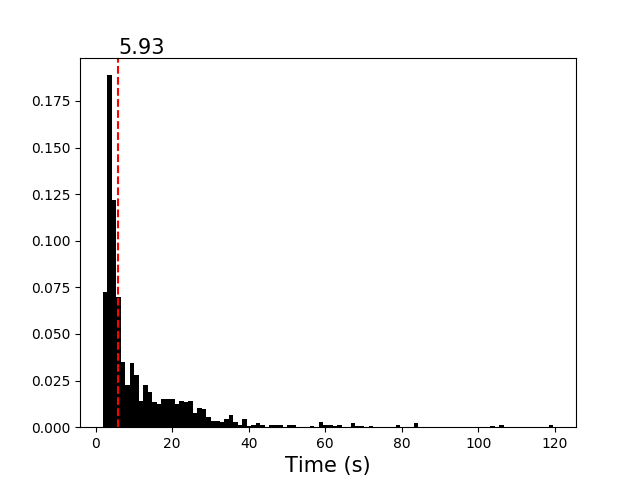
\includegraphics[width=0.32\textwidth]{figs/dstats/dan_melodic_line.png}
        \label{fig:ch4:melodic_line_dan}}
    \subfloat[Dan syllable]{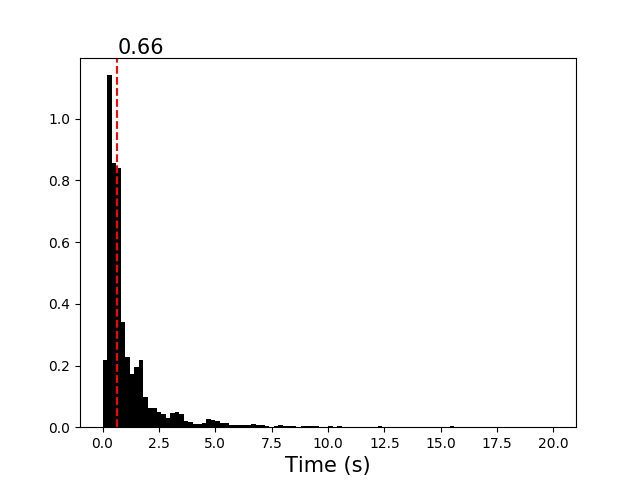
\includegraphics[width=0.32\textwidth]{figs/dstats/dan_syllable.png}
        \label{fig:ch4:syllable_dan}}
    \subfloat[Dan phoneme]{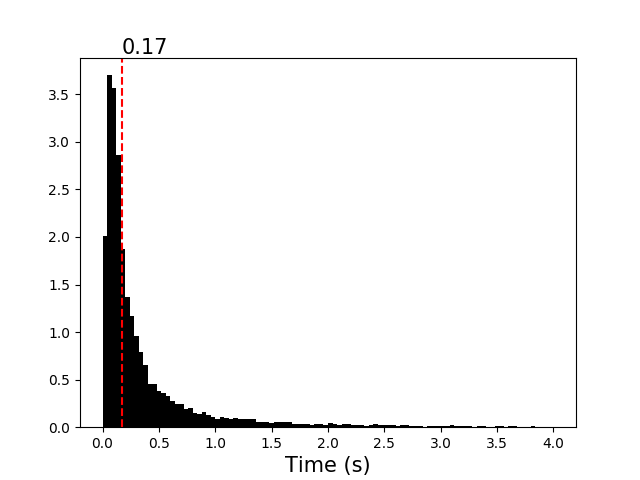
\includegraphics[width=0.32\textwidth]{figs/dstats/dan_phoneme.png}
        \label{fig:ch4:phoneme_dan}}
    \hfill
    \subfloat[Laosheng melodic line]{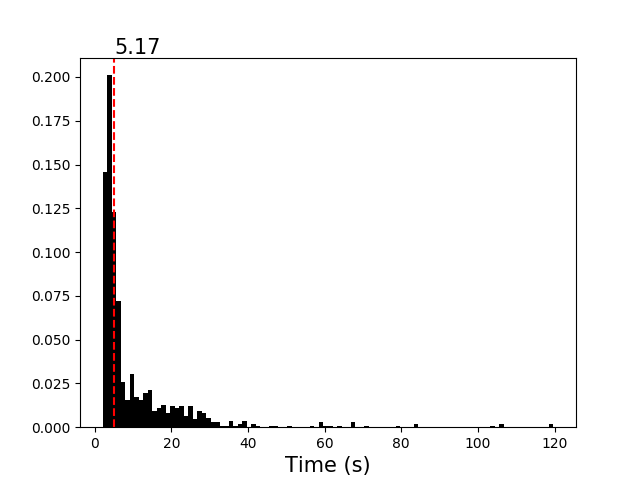
\includegraphics[width=0.32\textwidth]{figs/dstats/laosheng_melodic_line.png}
        \label{fig:ch4:melodic_line_laosheng}}
    \subfloat[Laosheng syllable]{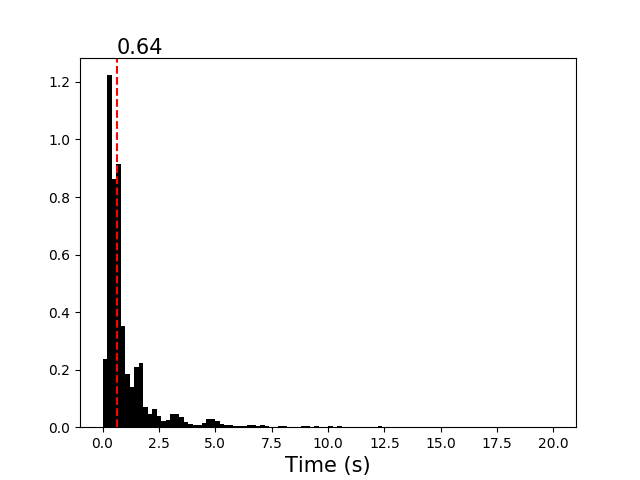
\includegraphics[width=0.32\textwidth]{figs/dstats/laosheng_syllable.png}
        \label{fig:ch4:syllable_laosheng}}
    \subfloat[Laosheng phoneme]{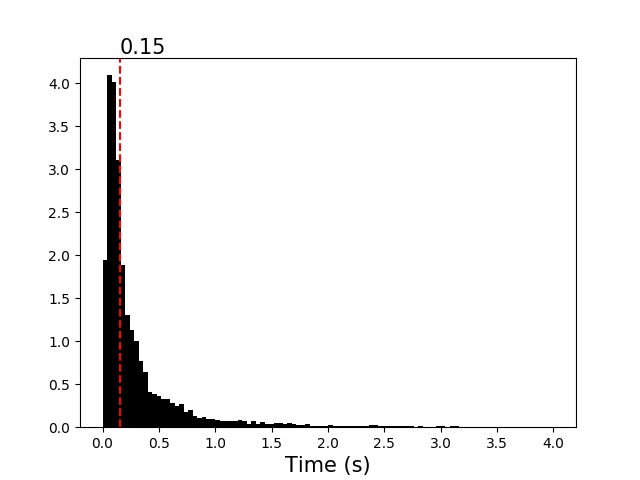
\includegraphics[width=0.32\textwidth]{figs/dstats/laosheng_phoneme.png}
        \label{fig:ch4:phoneme_laosheng}}
  
    \caption[]{Dan and laosheng melodic line, syllable and phoneme duration histograms normalized to unit density. Vertical red dash lines indicate the median duration.}
    \label{fig:ch4:dan_laosheng_histo}
\end{figure}

\figref{fig:ch4:dan_laosheng_histo} shows the duration histograms of melodic line, syllable and phoneme for dan and laosheng role-types. The general shapes of the histogram distribution between dan and laosheng are similar. Although there are prominent peaks on all the histograms, the durations are varied, which can be observed by the extended long-tails on each histogram. For example, the median melodic line duration of dan is 5.93s. However, a significant amount of melodic lines are longer than 10s; the median phoneme duration of laosheng is 0.15s, whereas those phonemes whose durations are more prolonged than 0.4s are not the minority.

\begin{figure}[ht!]
    \centering
    \subfloat[c]{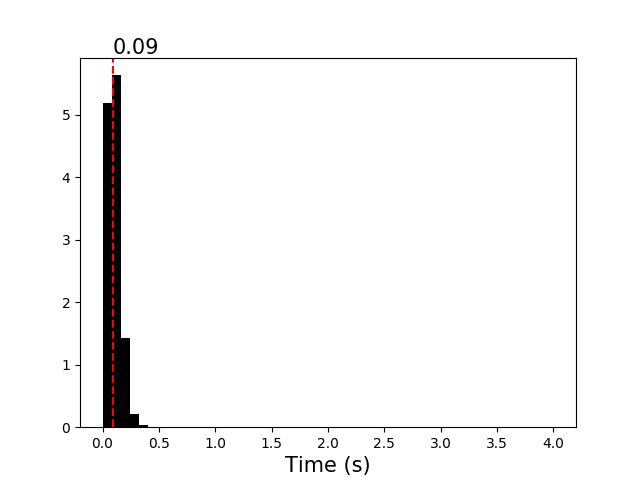
\includegraphics[width=0.43\textwidth]{figs/dstats/dan_c.png}
        \label{fig:ch4:c_dan}}
    \subfloat[l]{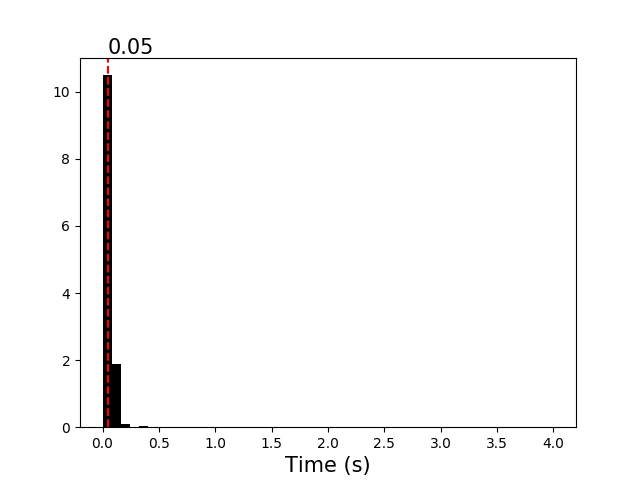
\includegraphics[width=0.43\textwidth]{figs/dstats/dan_l.png}
        \label{fig:ch4:l_dan}}
    \hfill

    \subfloat[N]{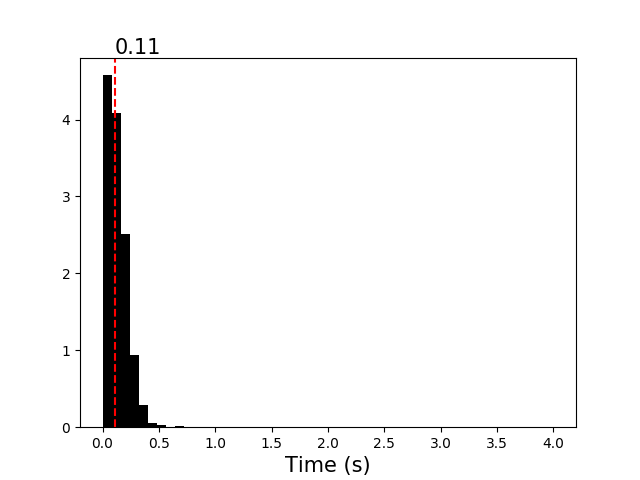
\includegraphics[width=0.43\textwidth]{figs/dstats/dan_N.png}
        \label{fig:ch4:N_dan}}
    \subfloat[@n]{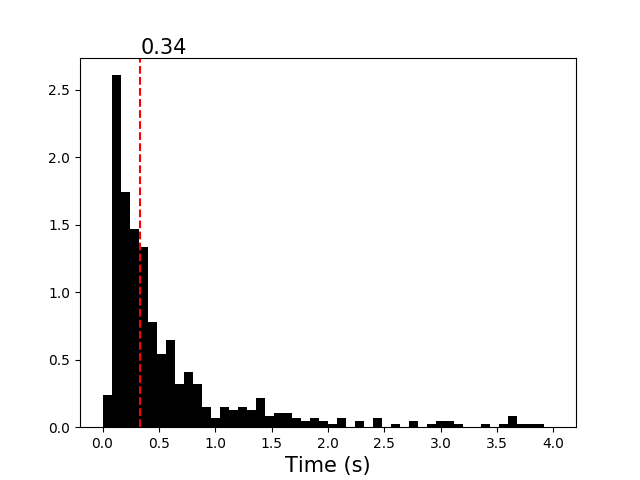
\includegraphics[width=0.43\textwidth]{figs/dstats/dan_@n.png}
        \label{fig:ch4:@n_dan}}
    \hfill
    \subfloat[i]{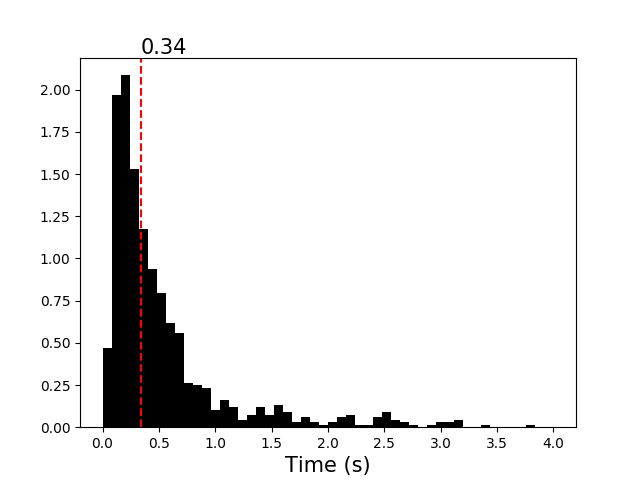
\includegraphics[width=0.43\textwidth]{figs/dstats/dan_i.png}
        \label{fig:ch4:i_dan}}
    \subfloat[a]{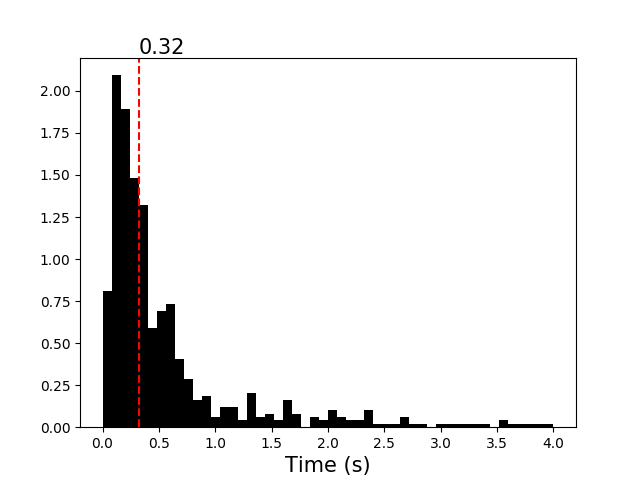
\includegraphics[width=0.43\textwidth]{figs/dstats/dan_a.png}
        \label{fig:ch4:a_dan}}
  
    \caption[]{Dan histograms normalized to the unit density of durations for phonemes c, l, N, @n, i, a. Vertical red dash lines are the median phoneme durations.}
    \label{fig:ch4:dan_histo_phoneme}
\end{figure}

\begin{figure}[ht!]
    \centering
    \subfloat[c]{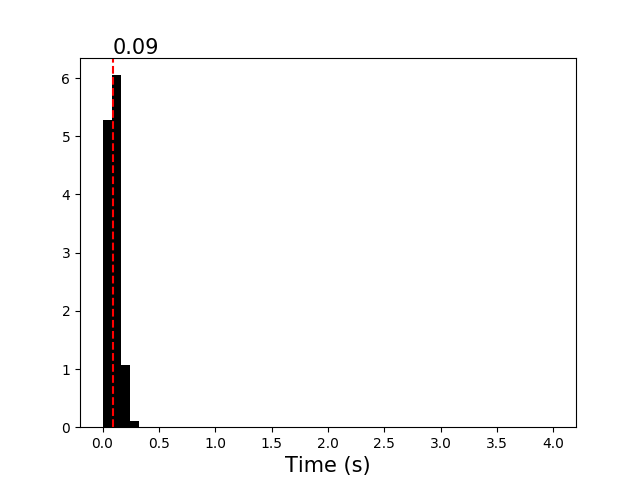
\includegraphics[width=0.43\textwidth]{figs/dstats/laosheng_c.png}
        \label{fig:ch4:c_laosheng}}
    \subfloat[l]{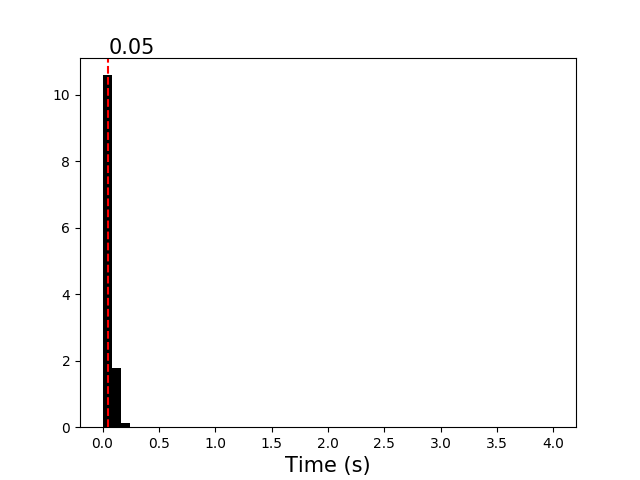
\includegraphics[width=0.43\textwidth]{figs/dstats/laosheng_l.png}
        \label{fig:ch4:l_laosheng}}
    \hfill

    \subfloat[N]{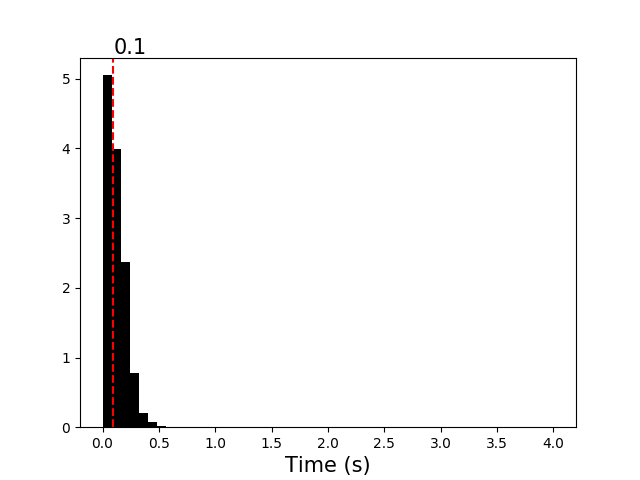
\includegraphics[width=0.43\textwidth]{figs/dstats/laosheng_N.png}
        \label{fig:ch4:N_laosheng}}
    \subfloat[@n]{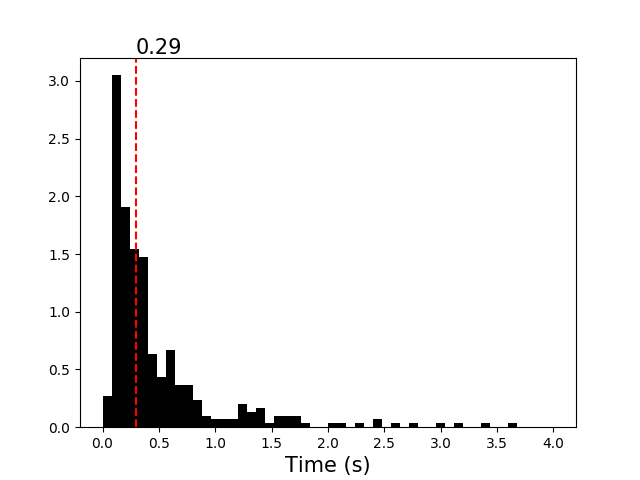
\includegraphics[width=0.43\textwidth]{figs/dstats/laosheng_@n.png}
        \label{fig:ch4:@n_laosheng}}
    \hfill
    \subfloat[i]{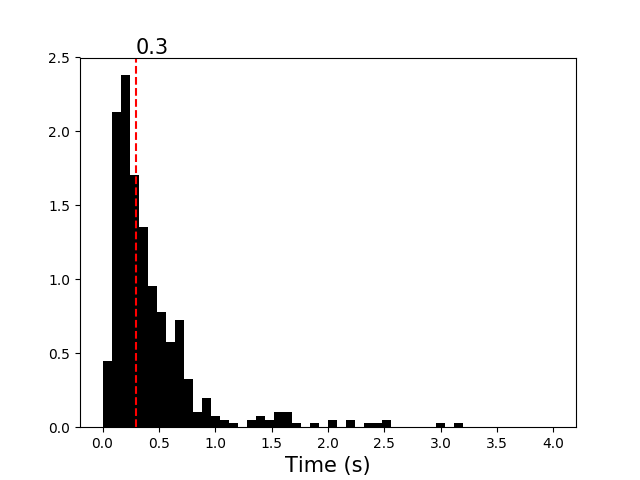
\includegraphics[width=0.43\textwidth]{figs/dstats/laosheng_i.png}
        \label{fig:ch4:i_laosheng}}
    \subfloat[a]{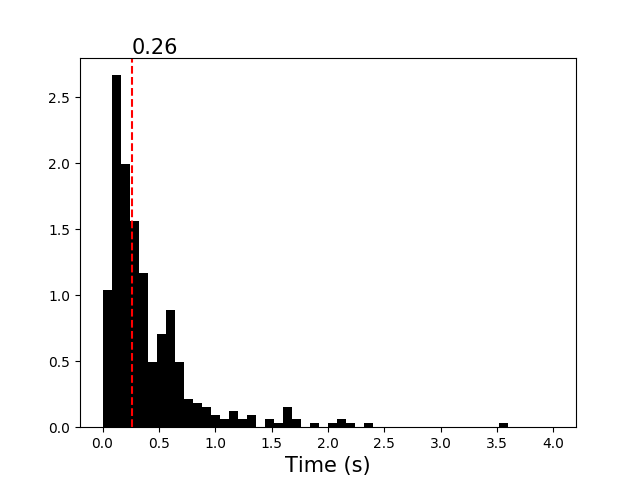
\includegraphics[width=0.43\textwidth]{figs/dstats/laosheng_a.png}
        \label{fig:ch4:a_laosheng}}
  
    \caption[]{Laosheng histograms normalized to the unit density of durations for phonemes c, l, N, @n, i, a. Vertical red dash lines are the median phoneme durations.}
    \label{fig:ch4:laosheng_histo_phoneme}
\end{figure}

\figref{fig:ch4:dan_histo_phoneme} and \figref{fig:ch4:laosheng_histo_phoneme} show the histograms of durations for the individual phoneme. The phonemes which we are selected to show are c, l, N, @n, i, a, in X-SAMPA format. c is an ensemble phoneme class of non-voiced consonants; l is a voiced phoneme; N is a terminal consonant; @n is a diphthong used as the central vowel in a syllable; i and a are single vowels also used as the central vowel in a syllable. Again, the general shapes of the histogram distribution between dan and laosheng are similar. The median duration of the individual phoneme of dan is longer than that of laosheng except for syllable initial consonants -- c and l. The duration of initial consonants does not vary much. However, the central vowels show a large duration variation since which are the primary part of a syllable sung by a singer in a prolonged way.

\section{Test datasets}\label{sec:ch4:test_datasets}
The test datasets are designed for special research tasks. There are several test datasets built in CompMusic for different musical traditions\footnote{\url{http://compmusic.upf.edu/datasets}}. We describe in this section only the test datasets for the tasks of automatic assessment of jingju singing pronunciation.

\subsection{Dataset for automatic syllable and phoneme segmentation}\label{sec:ch4:dataset_segmentation}

Automatic syllable and phoneme segmentation task require the data having syllable and phoneme time boundary and label annotations. Thus, we select the recordings with associated annotations in the corpus to form the test datasets. Two datasets are prepared -- ASPS\textsubscript{1} and ASPS\textsubscript{2}. ASPS\textsubscript{1} will be used for setting the baseline syllable and phoneme segmentation model, while ASPS\textsubscript{2} will be applied for searching an efficient state of the art syllable segmentation model.

ASPS\textsubscript{1} is a subset of the jingju a cappella singing corpus. The recordings in this dataset are selected from all three parts of the corpus. ASPS\textsubscript{1} contains two jingju role-types: \textit{dan} and \textit{laosheng}. 

\begin{table}[ht]
    \centering
    \begin{tabular}{l|cccc}
        \toprule
        & \#Recordings & \#Melodic line & \#Syllables & \#Phonemes \\
        \midrule
        Train           & 56 & 214 & 1965 & 5017 \\
        Test               & 39 & 216 & 1758 & 4651  \\
        \bottomrule
    \end{tabular}
    \caption{Statistics of the ASPS\textsubscript{1} test dataset.}
    \label{table:ch4:detailInfoDataset_asps_1}
\end{table}

The dataset contains 95 recordings split into train and test sets (table \ref{table:ch4:detailInfoDataset_asps_1}). The recordings in the test set only include student imitative singing. The corresponding teacher's demonstrative recordings can be found in the train set, which guarantees that the coarse syllable/phoneme duration and labels are available as a priori information being used in model testing. Recordings are pre-segmented into melodic line units. The syllable/phoneme ground truth boundaries (onsets/offsets) and phoneme labels are manually annotated. 29 phoneme categories are annotated, which include a silence category and a non-identifiable phoneme category, e.g. throat-clearing sound. The category table can be found in the Github page\footnote{\label{ft:github}\url{https://github.com/ronggong/interspeech2018_submission01}}. The dataset is publicly available\footnote{\url{https://doi.org/10.5281/zenodo.1185123}}.

\begin{table}[ht]
    \centering
    \begin{tabular}{l|ccc}
        \toprule
        & \#Recordings & \#Melodic line & \#Syllables \\
        \midrule
        Train           & 85 & 883 & 8368  \\
        Test               & 15 & 133 & 1203  \\
        \bottomrule
    \end{tabular}
    \caption{Statistics of the ASPS\textsubscript{2} test dataset.}
    \label{table:ch4:detail_info_jingju_dataset_asps_2}
\end{table}

ASPS\textsubscript{2} test dataset is also a subset of the jingju a cappella singing corpus. It also includes recordings of dan and laosheng role-types. ASPS\textsubscript{2} contains 100 recordings manually annotated for each syllable onset. The syllable segmentation evaluation will be conducted on each melodic line which has been pre-segmented manually. The statistics and train-test sets split are shown in table \ref{table:ch4:detail_info_jingju_dataset_asps_2}. It is worth to mention that the artists, recording rooms and recording equipment used for the test set is completely different from the training set. This train-test split setup avoids the artist/room/equipment filtering effects which might be happening in the evaluation process\cite{Flexer2010}. The musical score is also included in this dataset, which provides the syllable duration prior information for the evaluation. This dataset is openly available\footnote{\url{https://doi.org/10.5281/zenodo.1341070}\label{fn:jingju_dataset}}.

As it has been mentioned in \secref{sec:ch3:challenges}, pronunciation is a subconcept of the timbre, and in a signal point of view, timbre is related to the spectral envelope shape and the time variation of spectral content. In the following of this section, we show several spectrogram examples of various phoneme categories -- syllable initial non-voiced consonant, voiced consonant, medial vowel, central vowel and syllable terminal consonant, and the transition between two phonemes such as from syllable initial non-voice consonant to media vowel and from central vowel to syllable terminal consonant.

\begin{figure}[ht!]
    \centering
    \subfloat[Mel spectrogram of syllables ``hua, jie, shen".]{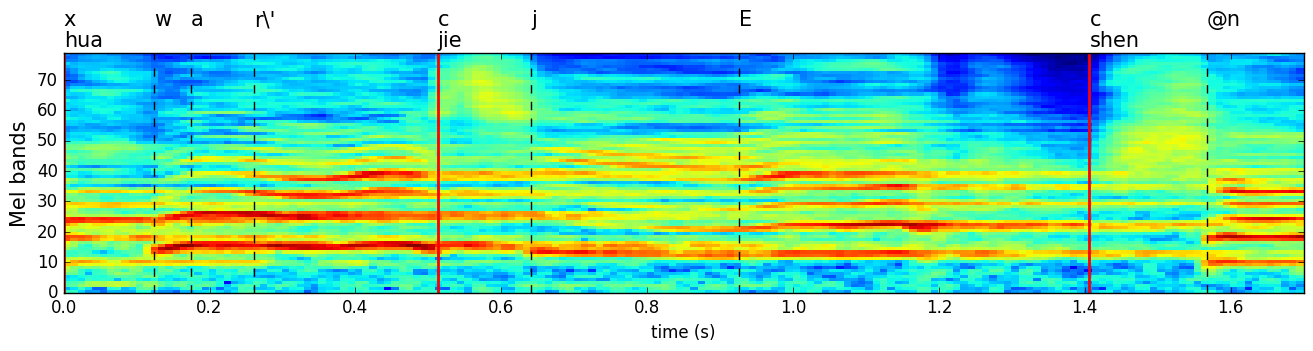
\includegraphics[width=\textwidth]{figs/dstats/spectro_hua_jie_shen.png}
        \label{fig:ch4:hua_jie_shen}}
    \hfill
    \subfloat[Mel spectrogram of syllables ``lai, li, hua".]{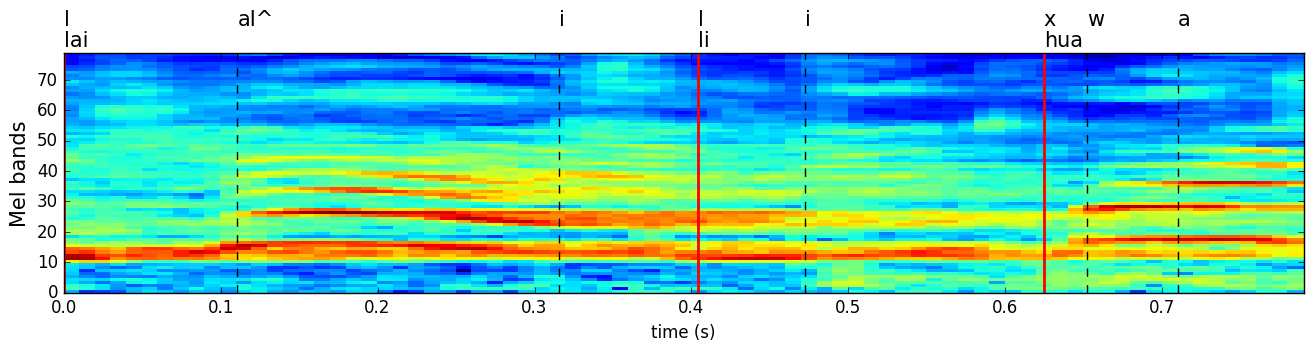
\includegraphics[width=\textwidth]{figs/dstats/spectro_lai_li_hua.png}
        \label{fig:ch4:lai_li_hua}}
    \hfill

    \subfloat[Mel spectrogram of syllables ``da, dan, ren".]{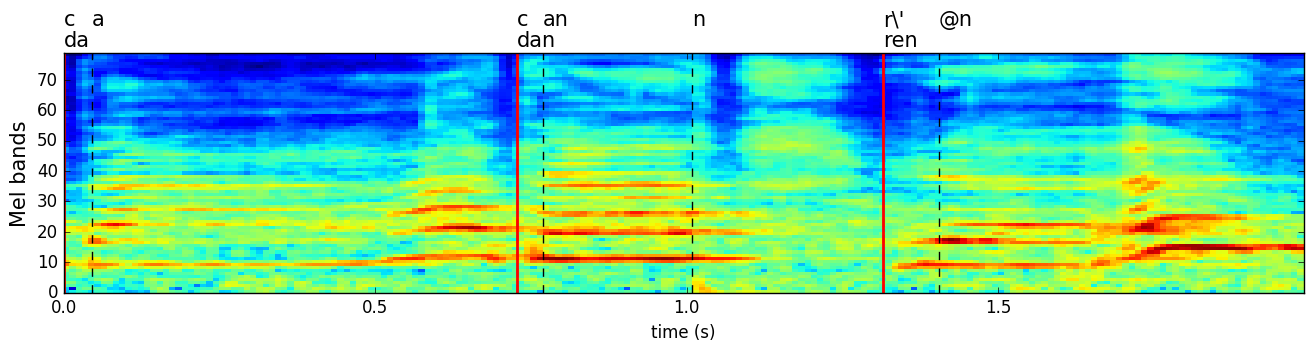
\includegraphics[width=\textwidth]{figs/dstats/spectro_da_dan_ren.png}
        \label{fig:ch4:da_dan_ren}}
  
    \caption[]{Three examples of syllablic Mel spectrogram. Vertical red solid lines are syllable onsets; vertical black dash lines are phoneme onsets.}
    \label{fig:ch4:task1_visualization}
\end{figure}

\figref{fig:ch4:task1_visualization} show three Mel spectrograms of singing syllable sequence, each of which consists of three syllables. We focus the analysis of the middle syllable of each sequence such that the transition between the first and second syllables and the transition between the second and third syllables can be visualized easily. 

The pinyin of middle syllable in \figref{fig:ch4:hua_jie_shen} is ``jie", which consists of three phonemes -- non-voiced consonant ``c", medial vowel ``j" and central vowel ``E". The spectrogram pattern of the non-voiced consonant ``c" can be distinguished easily from ``j" and ``E" by the high-frequency noise-like content since the consonant ``c" is an affricate. The spectrogram pattern of the central vowel ``E" contains more regular harmonic pattern than the medial vowel ``j". However, the difference between the patterns of ``j" and ``E" is not that obvious to discriminate.
 
The pinyin of the middle syllable in \figref{fig:ch4:lai_li_hua} is ``li", which consists of two phonemes -- syllable initial voiced consonant ``l" and the central vowel ``i". The difference of spectrogram pattern between these two phonemes can be hardly distinguished.

The pinyin of the middle syllable in \figref{fig:ch4:da_dan_ren} is ``dan", which consists of three phonemes -- syllable initial non-voiced consonant ``c", central vowel ``an" and syllable terminal consonant ``n". The consonant ``c" is a short non-voiced stop which doesn't contain harmonics. Thus, it can be distinguished easily from the central vowel ``an". The syllable terminal consonant ``n" doesn't contain any higher harmonics. Therefore, it can be distinguished easily as well from the central vowel ``an".

Given the analysis of the above three spectrogram examples, we can design the methodologies for the syllable and phoneme segmentation task in an intuitive way. Firstly, as most of the phoneme categories can be distinguished between each other except for medial vowel-central vowel and voiced consonant-central vowel, we can develop the segmentation algorithm based on the discrimination between phonemes. Secondly, as there are usually obvious spectrogram pattern transitions between phoneme segments, we can also devise the algorithm based on the detection of these transitions. The segmentation algorithms development and evaluation will be presented in detail in the next Chapter.

\subsection{Dataset for mispronunciation detection}\label{sec:ch4:dataset_mispronunciation}

As we have mentioned in \secref{sec:ch3:mispronunciation}, we consider only two types of mispronunciation in jingju singing -- the mispronunciation of special pronunciation and that of jianzi. The first type of mispronunciation -- special pronunciation, is that some written characters in jingju singing pieces should be pronounced differently than in Mandarin Chinese, however, the student doesn't pronounce them correctly as in teacher's demonstrative singing. The second type of mispronunciation -- jianzi, is that certain rounded syllables (团子, pinyin: tuanzi) in jingju singing pieces can be altered to pronounce as the pointed sounds (尖子, pinyin: jianzi), however, the student doesn't pay attention and still pronounce them as rounded syllables. 

In the actual jingju teaching scenario, the teacher's demonstrative singing pieces are given, thus we can identify in advance those special pronounced and jianzi written characters in the pieces. After we obtain the student's imitative singing pieces, the detection process can be carried out only on those special pronounced and jianzi written characters. To this end, we need a model which either can transcribe orthographically each singing syllables considering the special pronunciations and jianzi, or can distinguish between the standard Mandarin pronunciations and the special pronunciations/jianzi. Either way, we need a test dataset where the special pronounced syllables and jianzi are annotated orthographically in pinyin and in phoneme using X-SAMPA format.

\begin{table}[ht]
    \centering
    \begin{tabular}{l|ccccc}
        \toprule
        & \makecell{\#Melodic\\line} & \#Syl. & \makecell{\#Special\\pronunciation} & \#jianzi & \#Phn. \\
        \midrule
        Train           & 662 & 5797 & 463 & 41 & 15287 \\
        Test               & 345 & 3106 & 356 & 13 & 7561 \\
        \bottomrule
    \end{tabular}
    \caption{Statistics of the MD test dataset. Syl.: syllable; Phn.: phoneme.}
    \label{table:ch4:detailInfoDataset_md}
\end{table}

The Mispronunciation Detection -- MD test dataset is annotated for the above purpose. MD is a subset of the jingju a cappella singing corpus. The recordings in this dataset are selected mainly from the part 1 and 2 of the corpus. \tabref{table:ch4:detailInfoDataset_md} shows the statistics of the MD test dataset which are split into train and test parts, and the test part contains only the recordings of amateur singings. As we can see from the table, the occurrence of the special pronounced syllables is much larger than jianzi. Most importantly, in the test part of the MD dataset, according to the teacher's demonstrative recordings, there are in total 451 syllables of special pronunciation and 50 syllables of jianzi should be pronounced correctly by the students. However, in the actual recordings of the test part of the MD dataset, there are 102 syllables of special pronunciation and 37 syllables of jianzi which have been mispronounced, and 349 syllables of special pronunciation and 13 syllables of jianzi which have been pronounced correctly. These mispronounced syllables are labeled manually by comparing the annotation of the test recording and that of the corresponding teacher's demonstrative recording. For example, if in the teacher's recording, there is a special pronunciation /ngo/ for the syllable ``wo”, however, in the amateur's recording, the corresponding syllable is still pronounced as /wo/, this syllable is labeled as a mispronunciation.


\begin{figure}[ht!]
\makebox[\textwidth][c]{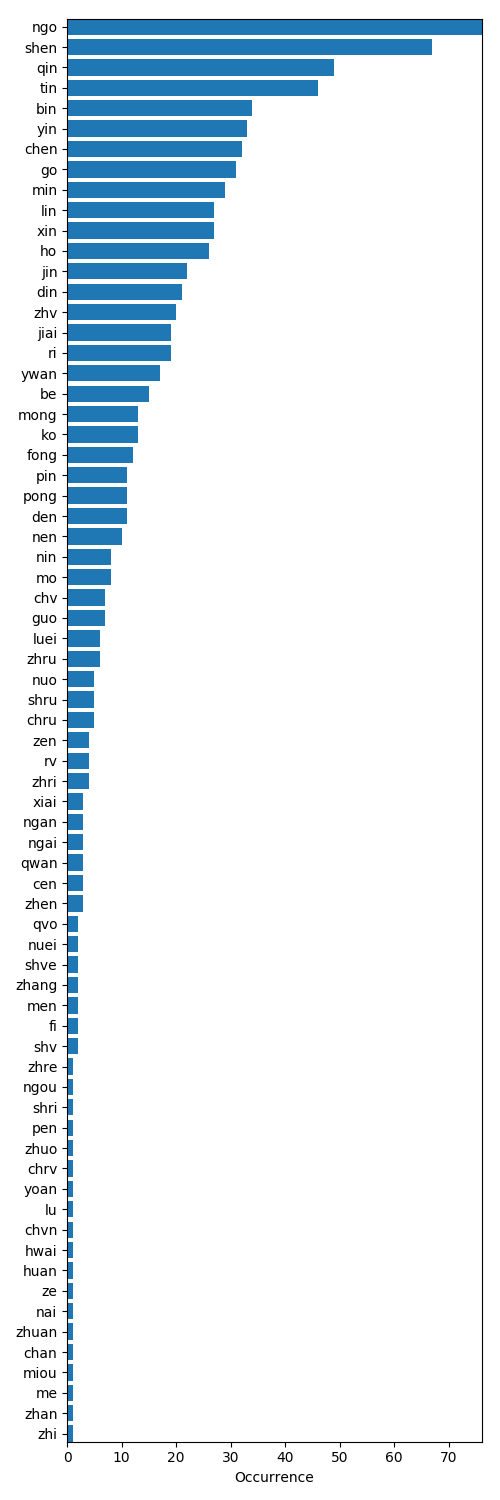
\includegraphics[width=0.6\textwidth]{figs/dstats/occurrence_special.png}}
\caption{The occurrence of each special pronounced syllable.}
\label{fig:ch4:occurrence_special}
\end{figure}

\figref{fig:ch4:occurrence_special} shows the occurrence of each special pronounced syllables in MD dataset. The most frequently occurred syllables are /ngo (我), shen, qin, tin, bin, yin, chen, go, min, lin, xin, ho/. The pronunciation /ngo/ is altered from /wo/ in standard Mandarin by changing the semivowel /w/ to the nasal consonant /ng/. The syllables /go/ and /ho/ are altered from /ge/ and /he/ in standard Mandarin by changing the vowel /e/ to /o/. The other syllables mentioned above are the alteration from velar nasal to alveolar nasal, for example, changing from /eng/ and /ing/ to /en/ and /in/. The full table of the alteration from Mandarin pronunciation to the special pronunciation appeared in the MD test dataset is presented in \tabref{tab:app:special_pronun}.

\begin{figure}[ht!]
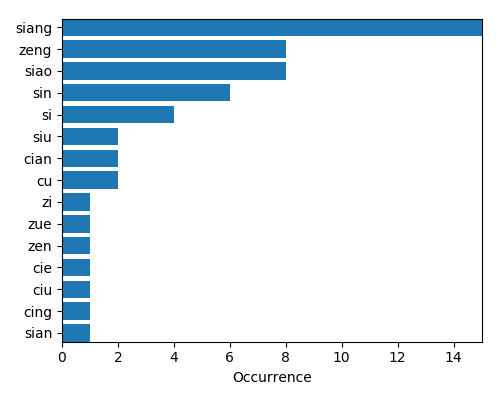
\includegraphics[width=\textwidth]{figs/dstats/occurrence_jianzi.png}
\caption{The occurrence of each jianzi syllable.}
\label{fig:ch4:occurrence_jianzi}
\end{figure}

\figref{fig:ch4:occurrence_jianzi} shows the occurrence of each jianzi in MD dataset. As we have mentioned in \secref{sec:ch2:jiantuanzi}, the rule of this pronunciation alteration is /j, zh/ -> /z/, /q, ch/ -> /c/, /x, sh/ -> /s/. For example, the pronunciation /siang/ is altered from /xiang/, and /zeng/ is altered from /zheng/. The full table of rounded syllables to the special pronunciation appeared in the MD test dataset is presented in \tabref{tab:app:jianzi}.

\subsection{Dataset for pronunciation and overall quality similarity measures}\label{sec:ch4:poqsm_dataset}

The test dataset for the task of pronunciation and overall quality similarity measures (POQSM) needs to have phoneme-level onset and offset time boundary and label annotation. These recordings are also a subset of the jingju a cappella singing corpus. The phoneme segments of the dataset are randomly split into the train, validation and test sets, except that we deliberately use the recordings of the amateurs of jingju groups in community activity centers (see \secref{sec:ch4:jingju_acappella_singing_corpus} for the information of the recording artists of the corpus) as the amateur part of the test set. The purpose of using this special amateur part of the test set is to avoid artist and room filtering effects by checking if the trained assessment model overfits on certain singers or the acoustic room conditions of the train and validation sets.

\begin{landscape}
\mbox{}\vfill
\begin{table}[ht!]
\centering
\begin{tabular}{l|c|c|c|c}
\toprule
           & \makecell{\#Professional\\phonemes} & \makecell{\#Amateur\\phonemes} & Professional singers                                        & Amateur singers                                 \\
\midrule
Train      & 6888                     & 5673                & \multirow{3}{*}{\makecell{Adult\\conservatory students\\or graduates}} & \multirow{2}{*}{Mainly primary school students} \\
\cline{1-3}
Validation & 1733                     & 1429                &                                                             &                                                 \\
\cline{1-3}\cline{5-5}
Test       & 2167                     & 2021                &                                                             & Adult amateur singers \\
\bottomrule
\end{tabular}
\caption{POQSM test dataset split, numbers of the professional and amateur singing phonemes and the source of the professional and amateur singers.}
\label{tab:ch4:exp_dataset_poqsm}
\end{table}
\vfill
\end{landscape}

We consider the fact that, after dataset splitting, the train, validation and test sets would contain both professional and amateur phoneme segments. Additionally, the amateur part of the train and validation sets mainly include the phoneme segments of the primary school students, while that of the test set contains exclusively the segments of the adult singers recorded in a different room (see the room iv in section \ref{sec:ch4:recording_setup}). This special split of the test set would verify the artist or room filtering effect of the assessment model \cite{Flexer2010}. Please check table \ref{tab:ch4:exp_dataset_poqsm} for the phoneme numbers and the singers in each split. For the detailed information on the phoneme numbers per phoneme class and recording file names used for each split, please consult this link\footref{foot:zenodo_dlfm2018}. The test dataset can be download in this link\footnote{\url{https://doi.org/10.5281/zenodo.1287251}\label{foot:zenodo_dlfm2018}}.

An example of spectrogram visualization between teacher and student singing melodic line has been presented already in \secref{sec:ch3:char_singing}. In such an example, although the student does not commit any mispronunciation, there still exists a significant pronunciation quality and an overall quality gap between her singing and the teacher singing. Building a pronunciation and overall quality similarity model can help detect the relevant singing problems automatically apart from mispronunciation.

\makeatletter
\def\BState{\State\hskip-\ALG@thistlm}
\makeatother

\chapter{Automatic syllable and phoneme segmentation}\label{chap:segmentation}
% \begin{epigraphs}
%   \qitem{...the first beat (sam) is highly significant structurally, as it frequently marks the coming together of the rhythmic streams of soloist and accompanist, and the resolution point for rhythmic tension.}{\citeA[p. 81]{clayton:00:time}}
% \end{epigraphs}

Automatic syllable and phoneme segmentation of singing voice is an important MIR task. It provides preliminary syllable or phoneme time boundary and label information to achieve a fine-grained singing voice assessment.

Syllable and phoneme segmentation aim to time-align a piece of singing voice audio recording with syllable or phoneme sequence. It tags the recording with the time-aligned syllable or phoneme boundary timestamps and labels. Within the context of jingju music, syllable and phoneme segmentation aim to time-align a recording with a syllable sequence in pinyin format or a phoneme sequence in X-SAMPA format.

This chapter aims to address the automatic syllable and phoneme segmentation task within the context of jingju music, presenting several methods and an evaluation of these methods. The main aims of this chapter are:

\begin{enumerate}[leftmargin=*]

\item To address automatic syllable and phoneme segmentation task for jingju music. The problem is formulated in two ways -- duration-informed lyrics-to-audio alignment and duration-informed syllable or phoneme onset detection. Several approaches are proposed to address the problem.
\item To present a detailed description of hidden semi-Markov model-based (HSMM) segmentation method and the proposed onset detection-based method for syllable and phoneme segmentation.
\item To present an evaluation of HSMM-based alignment method and the proposed onset detection-based method and explore various deep learning architectures to improve the onset detection-based method.
\end{enumerate}

\section{Task description}\label{sec:ch5:description}

We describe the automatic syllable and phoneme segmentation task addressed in this dissertation. We will also describe how the set of approaches described in this chapter can be adapted to this task, making the task of syllable and phoneme segmentation flexible to the available audio recordings and the related annotations. The task description presented in this section is continued building on the problem formulation presented in \secref{sec:ch3:segmentation_formulation}. 

Given the singing audio recording pre-segmented into pieces of melodic line level, and the prior coarse syllable or phoneme duration information extracted from the musical score or the annotation of teacher's recording, the most relevant syllable and phoneme segmentation tasks for jingju music are duration-informed lyrics-to-audio alignment or duration-informed syllable or phoneme onset detection. In the context of jingju music, lyrics-to-audio alignment aims to time-align the a priori phoneme sequence in X-SAMPA format with the melodic line singing audio piece. The coarse phoneme duration information can be incorporated into the alignment system by using an HSMM-based model, which sets up the baseline segmentation system stemmed from various HMM-based text-to-speech alignment and lyrics-to-audio alignment methods presented in \secref{sec:ch2:text_speech_alignment} and \secref{sec:ch2:lyrics_audio_alignment}. Syllable and phoneme onset detection aim to find the onset timestamps for the syllables and phonemes in a melodic line singing audio piece. The a priori syllable and phoneme duration information can be used as a post-processing step in the detection algorithm to help select the correct onsets. In the context of this dissertation, because the a priori duration information is always accompanied with syllable or phoneme label, the post-processing onset selection method using a priori duration information is equal to time-aligning the syllable or phoneme sequence with the melodic line singing audio piece. 

The two main tasks of this chapter are setting up the HSMM-based baseline segmentation method and proposing the onset detection-based segmentation method. As the third task of this chapter, we explore various deep learning architectures for the syllable onset detection and try to identify and explain the most efficient architecture. The performance of all the three tasks will be evaluated on ASPS\textsubscript{1} and ASPS\textsubscript{2} test datasets. The results and the pros and cons of two segmentation methods and various deep learning architectures will be discussed in detail.

\section{Prerequisite processing}

In this section, we present two prerequisite processings that will be used in the segmentation approaches -- logarithmic Mel input representation and a priori coarse duration model. The former converts the singing voice audio waveform to a perceptual representation - Mel spectrogram, which is then used as the input representation of both HSMM-based and onset detection-based segmentation methods. The latter utilizes the coarse syllable or phoneme durations extracted from the annotation of teacher's recording to build the duration model, as the teacher's recording and its annotation is always prior information for an assessment system. The phoneme duration model is then integrated into the HSMM-based segmentation method as the state occupancy distribution, and the syllable and phoneme duration models are both used in the onset detection-based segmentation method to help select the correct syllable and phoneme onsets.

\subsection{Logarithmic Mel input representation}\label{sec:ch5:input_representation}

We use \textsc{Madmom}\cite{Bock2016} Python package to calculate the log-mel spectrogram of the singing voice audio. The frame size and hop size of the spectrogram are respectively 46.4ms (2048 samples) and 10ms (441 samples). The low and high frequency bounds of the log-mel calculation are 27.5Hz and 16kHz. We use log-mel input features with a overlapped context window of 15 frames and 80 bins as the input to the networks. The classification acoustic model used in HSMM-based segmentation task takes a categorical phoneme label for every context window. While the onset detection model takes a binary onset/non-onset decision sequentially for every context window. This audio pre-processing configuration is almost the same as in Schl\"{u}ter and B\"{o}ck's work\cite{Schluter2014} except that 3 input channels with respectively frame sizes 23ms, 46ms and 93ms have been used in their work, whereas only 1 channel with frame size 46.4ms input is used in this research.

\subsection{Coarse duration and \textit{a priori} duration model}\label{sec:pp_coarse_duration}

The syllable durations of the teacher's singing phrase are stored in an array $M^s=\mu^{1} \cdots \mu^{n} \cdots \mu^{N}$, where $\mu^{n}$ is the duration of the nth syllable. The phoneme durations are stored in a nested array $M_p=M^{1}_p \cdots M^{n}_p \cdots M^{N}_p$, where $M^{n}_p$ is the sub-array with respect to the nth syllable and can be further expanded to $M^{n}_p=\mu_{1}^{n} \cdots \mu_{k}^{n} \cdots \mu_{K_{n}}^{n}$, where $K_{n}$ is the number of phonemes contained in the nth syllable. The phoneme durations of the nth syllable sum to its syllable duration: $\mu^{n}=\sum_{k=1}^{K_{n}} \mu_k^{n}$ (figure \ref{fig:coarse_dur}). In both syllable and phoneme duration sequences -- $M^s$, $M_p$, the duration of the silence is not treated separately and is merged with its previous syllable or phoneme.

\begin{figure}[ht!]
    \centering
    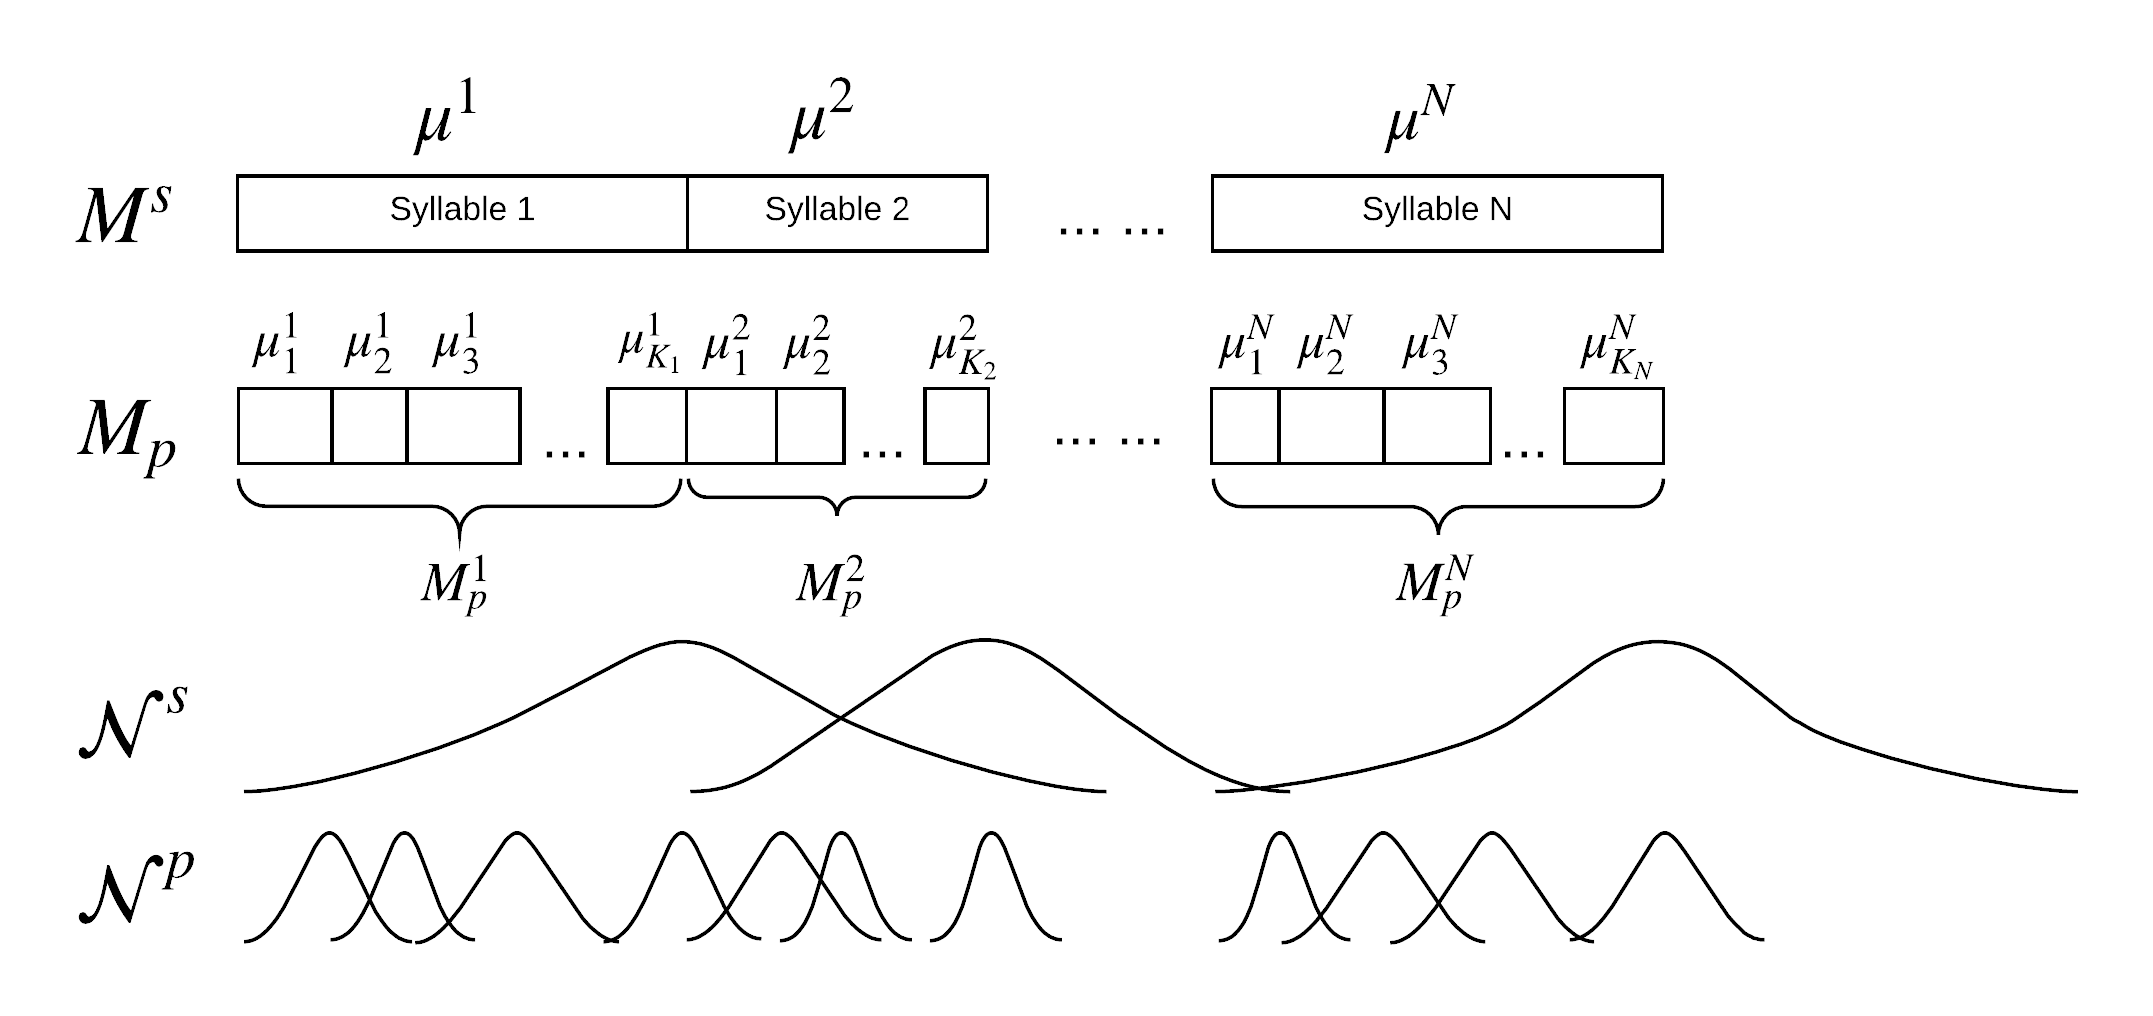
\includegraphics[width=\textwidth]{figs/blockDiags_rong/ch5_coarse_durations_segmentation.png}
    \caption{Illustration of the syllable $M^s$ and phoneme $M_p$ coarse duration sequences and their \textit{a priori} duration models -- $\mathcal{N}^s$, $\mathcal{N}^p$. The blank rectangulars in $M_p$ represent the phonemes.}
    \label{fig:coarse_dur}
\end{figure}

The \textit{a priori} duration model is shaped with a Gaussian function $\mathcal{N} (d; {\mu}_n, \sigma_n^2)$. It provides the prior likelihood of an onset to occur according to the syllable/phoneme duration of the teacher's singing. The mean ${\mu}_n$ of the Gaussian represents the expected duration of nth teacher's syllable/phoneme. Its standard deviation $\sigma_n$ is proportional to $\mu_n$: $\sigma_n=\gamma \mu_n$ and $\gamma$ is heuristically set to 0.35. Figure \ref{fig:coarse_dur} provides an intuitive example of how the \textit{a priori} duration model works. The a priori phoneme duration model will be used as the state occupancy distribution in the HSMM-based segmentation method, and the a priori syllable and phoneme duration models will be incorporated into a duration-informed HMM as the state transition probabilities to inform that where syllable/phoneme onsets is likely to occur in student's singing phrase.

\section{HSMM-based segmentation method}

As a baseline, we develop an lyrics-to-audio alignment system which also makes use of the prior phoneme duration information. This lyrics-to-audio alignment system is a 1-state monophone DNN/HSMM model. We use monophone model because our small dataset doesn't have enough phoneme instances for exploring the context-dependent triphones model, also Brognaux and Drugman \cite{brognaux2016hmm} and Pakoci et al. \cite{pakoci2016phonetic} argued that context-dependent model can not bring significant alignment improvement. It is convenient to apply 1-state model because each phoneme can be represented by a semi-Markovian state carrying a state occupancy time distribution. The audio preprocessing step is presented in \secref{sec:ch5:input_representation}.

\subsection{Discriminative acoustic model}

We use a CNN with softmax outputs as the discriminative acoustic model. According to the work of Renals et al. \cite{Renals1994Connectionist}, a neural network with softmax outputs trained for framewise phoneme classification outputs the posterior probability $p(q|x)$ ($q$: state, $x$: observation), which can be approximated as the acoustic model at the frame-level if we assume equal phoneme class priors. In Pons et el.'s work \cite{Pons2017Timbre}, a one-layer CNN with multi-filter shapes has been designed. It has been experimentally proved that this architecture can successfully learn timbral characteristics and outperformed some deeper CNN architectures in the phoneme classification task for a small jingju singing dataset. The convoluational layer of the architecture has 128 filters of sizes $50{\times}1$ and $70{\times}1$, 64 filters of sizes $50{\times}5$ and $70{\times}5$, and 32 filters of sizes $50{\times}10$ and $70{\times}10$. These filters are large in the frequency axis and narrow in temporal axis, which are designed to capture timbral relevant time-frequency spectrogram context. A max-pool layer of $2{\times}N'$ follows before the 32-way softmax output layer with 30\% dropout, where $N'$ is the temporal dimension of the feature map. Max-pooling of $2{\times}N'$ was chosen to achieve time-invariant representations
while keeping the frequency resolution. The detailed model architecture is shown in \tabref{table:ch5:cnn_acoustic_model}.

\begin{table}[ht!]
\centering
\begin{tabular}{l}
\toprule
\makecell[l]{Layer1: Conv 128x $50{\times}1$, 64x $50{\times}5$, 32x $50{\times}5$\\128x $70{\times}1$, 64x $70{\times}5$, 32x $70{\times}10$} \\
Layer2: Max-pooling $2{\times}N'$ \\
Layer3: Dropout 0.3\\
Output layer: 29-way softmax\\
\bottomrule
\end{tabular}
\caption{One-layer CNN architecture of the acoustic model. N' is the temporal dimension of the feature map.}
\label{table:ch5:cnn_acoustic_model}
\end{table}

\subsubsection{Model training}

We use this one-layer CNN acoustic model for the baseline method. The log-mel context window representation presented in \secref{sec:ch5:input_representation} is used as the model input. The target labels of the training set are prepared according to the ground truth annotations. We set the label of a spectrogram context window to its categorical phoneme class. The model predicts the phoneme class posterior probability for each log-mel spectrogram context window.

The model parameters are learned with mini-batch training (batch size 256), adam \cite{kingma2014adam} update rule and early stopping -- if validation loss is not decreasing after 15 epochs. ELUs activation functions and weight decay regularization are used in the first convolutional layer.

\subsection{Coarse duration and state occupancy distribution}

The HSMM-based segmentation method receives the phoneme durations of teacher's singing phrase as the prior input. The phoneme durations are stored in a collapsed version of the $M^p$ array (section \ref{sec:pp_coarse_duration}): $M_c^p=\mu_{1}^{s1} \mu_{2}^{s1} \cdots \mu_{N_{s1}}^{s1} \cdots \mu_{1}^{sN} \mu_{2}^{sN} \cdots \mu_{N_{sN}}^{sN}$. The silences are treated separately and have their independent durations.

The state occupancy is the time duration of the phoneme state of the student's singing. It is expected in the best case to be the same duration as that of the teacher's singing. However, in the actual scenario, the phoneme duration of the student's singing always deviates from that of the teacher's singing in varying degrees. We build the state occupancy distribution as a Gaussian, which has the same form $\mathcal{N} (d; {\mu_n}, \sigma_n^2)$ as in section \ref{sec:pp_coarse_duration}, where $\mu_n$ indicates in this context the nth phoneme duration of the teacher's singing. We set $\gamma$ empirically to 0.2 as we found this value works well in our preliminary experiment.

We construct an HSMM for phoneme segment inference. The topology is a left-to-right semi-Markov chain, where the states represent sequentially the phonemes of the teacher's singing phrase. As we are dealing with the forced alignment, we constraint that the inference can only be started by the leftmost state and terminated to the rightmost state. The self-transition probabilities are set to 0 because the state occupancy depends on the predefined distribution. Other transitions -- from current states to subsequent states are set to 1. We use a one-layer CNN with multi-filter shapes as the acoustic model \cite{Pons2017Timbre} and the Gaussian $\mathcal{N} (d; {\mu_n}, \sigma_n^2)$ introduced in section \ref{sec:pp_coarse_duration} as the state occupancy distribution. The inference goal is to find best state sequence, and we use Gu\'{e}don's HSMM Viterbi algorithm \cite{GUEDON20072379} for this purpose. The baseline details and code can be found in the Github page\textsuperscript{\ref{ft:github}}. Finally, the segments are labeled by the alignment path, and the phoneme onsets are taken on the state transition time positions.

\subsection{Experimental setup}

We use ASPS\textsubscript{1} test dataset presented in \secref{sec:ch4:dataset_segmentation} and two metrics to evaluate the algorithm performance -- onset detection accuracy and percentage of correct segments, where we also consider the phoneme label correctness in calculating onset detection accuracy. These two metrics have been presented in \secref{sec:ch2:evaluation_metrics}. We trained the CNN acoustic model 5 times with different random seeds, and report the mean and the standard deviation score on the testing part of the dataset.

\subsection{Results and discussions}\label{sec:ch5:results_hsmm}

We only show the F1-measure of the results of the HSMM-based method in \tabref{table:ch5:results_hsmm}. The full results including precision and recall can be found in the Github page\textsuperscript{\ref{ft:github}}. The performance of the HSMM-based method is mediocre in the sense that none of the onset detection accuracy and percentage of correct segments reaches an ideal level. The low onset detection accuracy -- 44.5\% for phoneme detection, 41\% for syllable detection, means that the HSMM-based method cannot maintain more than half of the detected onsets within the 50ms tolerance window, which is crucial for the onset detection or segmentation of the consonants since they usually have a short duration. The low percentage of correct segments -- 53.4\% for phoneme and 65.8\% for syllable, means that many phoneme boundaries including vowel boundaries are not detected correctly. As a consequence, the segmentation error will propagate to the automatic assessment step and reduce the assessment accuracy. 

\begin{table}[ht]
  \centering
  \caption{Evaluation results table. Table cell: mean score$\pm$standard deviation score.}
  \label{table:ch5:results_hsmm}
  \begin{tabular}{cccc}
    \toprule
        \multicolumn{2}{c}{Onset F1-measure \%} & \multicolumn{2}{c}{Segmentation \%} \\
    phoneme & syllable &  phoneme & syllable \\
    \midrule
    44.5$\pm$0.9 & 41.0$\pm$1.0 & 53.4$\pm$0.9 & 65.8$\pm$0.7 \\
    \bottomrule
  \end{tabular}
\end{table}

\begin{figure}[ht!]
    \centering
    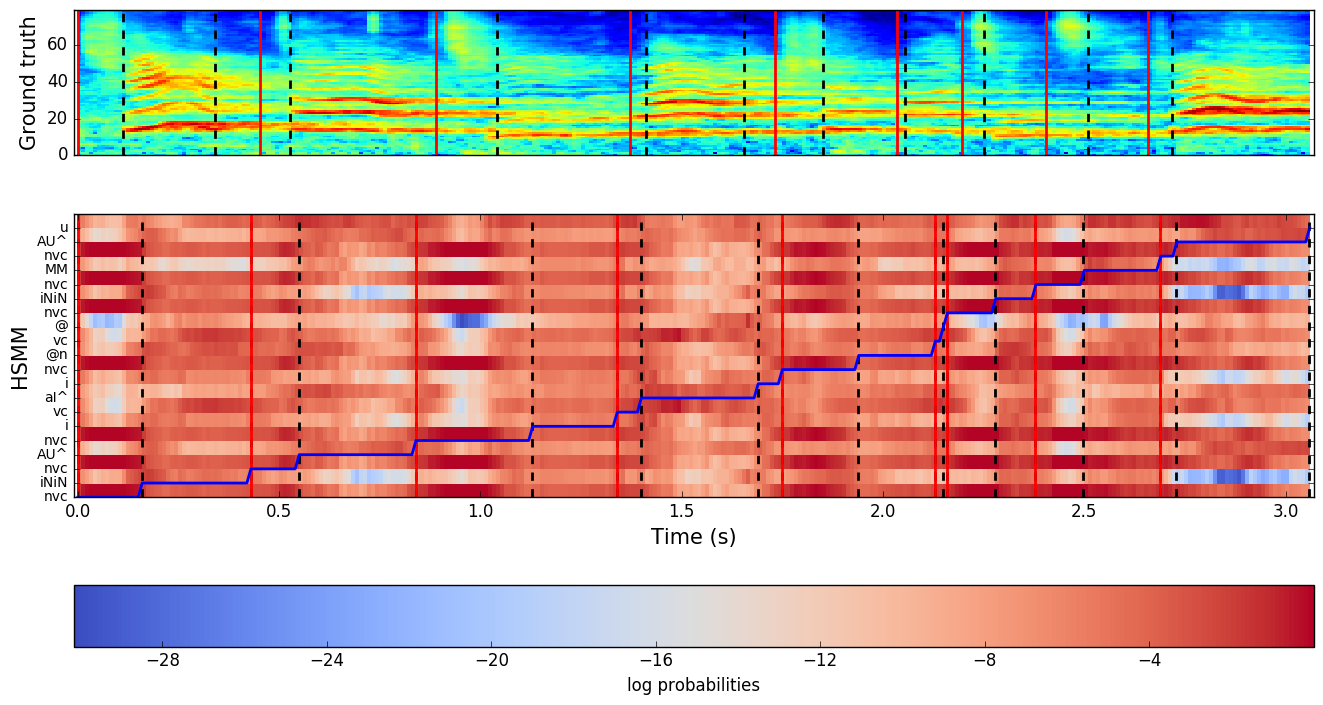
\includegraphics[width=\textwidth]{figs/results/ch5_results_hsmm_baseline.png}
    \caption{An illustration of the result for a singing phrase in the testing part of the dataset. The red solid and black dash vertical lines are respectively the syllable and phoneme onset positions. 1st row: ground truth, 2nd row: HSMM-based segmentation method. The staircase-shaped curve in the 2nd row is the alignment path.}
    \label{fig:ch5:results_example_hsmm}
\end{figure}

\figref{fig:ch5:results_example_hsmm} shows a result example for a singing phrase in the testing part of the dataset. Notice that there are some extra or missing onsets in the detection. This is due to the inconsistency between the coarse duration input and the ground truth, for example, students might sing extra or miss some phonemes in the actual singing. We can also observe the deviations between the detected and ground truth phoneme onsets. Some of the deviations are quite large, for example, the first detected syllable onset after 2 seconds in the 2nd row, which is an indication that the HSMM-based segmentation method cannot meet the need of having a precise segmentation, and it has to be improved or replaced by a better method. 

The unsatisfactory performance of the HSMM-based segmentation method might be due to the lack of a large training dataset. The DNN acoustic model usually requires a certain amount of training dataset such that it can effectively learn the temporal-spectral patterns of each phoneme class.

\section{Onset detection-based segmentation method}

The unsatisfactory performance of the HSMM-based segmentation method motivates us to search for a more accurate segmentation method. As we mentioned in \secref{sec:ch5:results_hsmm}, the lack of enough training dataset might be the cause of the unsatisfactory performance. In this section, we devise a coarse duration-informed syllable and phoneme segmentation method based on syllable and phoneme onset detection. As the onset detection is generally a binary detection problem -- to classify the spectrogram of each frame into onset or non-onset class, it can greatly reduce the amount of the required training dataset. The coarse syllable and phoneme durations extracted from the annotation of teacher's recording can be used in the algorithm to boost the segmentation performance.

In the proposed onset detection-based segmentation method, the syllable and phoneme onset detection functions (ODFs) are jointly learned by a hard parameter sharing multi-task CNN model. The syllable/phoneme boundaries and labels are then inferred by an HMM using the \textit{a priori} duration model as the transition probabilities and the ODFs as the emission probabilities.

\subsection{CNN onset detection function}\label{sec:ch5:cnn_odf}

We build a CNN for classifying each log-mel context and output the syllable and phoneme ODFs. We extend the CNN architecture presented in Schl\"{u}ter's work \cite{Schluter2014} by using two predicting objectives -- syllable and phoneme (figure \ref{fig:cnn_architecture}). The two objectives share the same parameters, and both are using the sigmoid activation function. Binary cross-entropy is used as the loss function. The loss weighting coefficients for the two objectives are set to equal since no significant effect has been found in the preliminary experiment.

\begin{figure}[ht!]
    \centering
    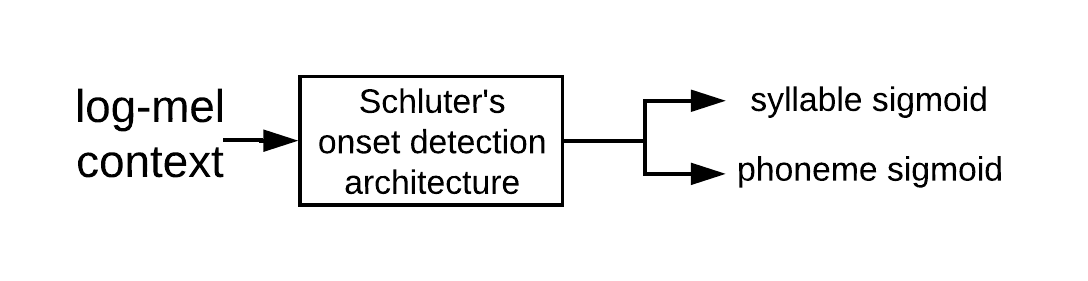
\includegraphics[width=\textwidth]{figs/blockDiags_rong/ch5_cnn_architecture_segmentation.png}
    \caption{Diagram of the multi-task CNN model.}
    \label{fig:cnn_architecture}
\end{figure}

\subsubsection{Model training}

The target labels of the training set are prepared according to the ground truth annotations. We set the label of a certain context to 1 if an onset has been annotated for its corresponding frame, otherwise 0. To compensate the human annotation inaccuracy and to augment the positive sample size, we also set the labels of the two neighbor contexts to 1. However, the importance of the neighbor contexts should not be equal to their center context, thus we compensate this by setting the sample weights of the neighbor contexts to 0.25. A similar sample weighting strategy has been presented in Schluter's paper \cite{Schluter2014}. Finally, for each log-mel context, we have its syllable and phoneme labels. They will be used as the training targets in the CNN model to predict the onset presence.

The model parameters are learned with mini-batch training (batch size 256), adam \cite{kingma2014adam} update rule and early stopping -- if validation loss is not decreasing after 15 epochs. The ODFs output from the CNN model is used as the emission probabilities for the syllable/phoneme boundary inference.

\subsection{Phoneme boundaries and labels inference}\label{sec:ch5:dur_label}

The inference algorithm receives the syllable and phoneme durations and labels of teacher's singing phrase as the prior input and infers the syllable and phoneme boundaries and labels for the student's singing phrase.

We present an HMM configuration which makes use of the coarse duration and label input (section \ref{sec:pp_coarse_duration}) and can be applied to inferring firstly (i) the syllable boundaries and labels on the ODF for the whole singing phrase, then (ii) the phoneme boundaries and labels on the ODF segment constrained by the inferred syllable boundaries. To use the same inference formulation, we unify the notations $N$, $K_n$ (both introduced in section \ref{sec:pp_coarse_duration}) to $N$, and $M^s$, $M^{n}_{p}$ to $M$. The unification of the notations has a practical meaning because we use the same algorithm for both syllable and phoneme inference. The HMM is characterized by the following:

\begin{enumerate}[leftmargin=*]
    \item The hidden state space is a set of $T$ candidate onset positions $S_1, S_2, \cdots, S_T$ discretized by the hop size, where $S_{T}$ is the offset position of the last syllable or the last phoneme within a syllable.
    \item The state transition probability at the time instant $t$ associated with state changes is defined by \textit{a priori} duration distribution $\mathcal{N} (d_{ij} ; \mu_t, \sigma_t^2)$, where $d_{ij}$ is the time distance between states $S_i$ and $S_j$ ($j>i$). The length of the inferred state sequence is equal to $N$.
    \item The emission probability for the state $S_j$ is represented by its value in the ODF, which is denoted as $p_j$.
\end{enumerate} 

The goal is to find the best onset state sequence $Q={q_1 q_2 \cdots q_{N-1}}$ for a given duration sequence $M$ and impose the corresponding segment label, where $q_i$ denotes the onset of the $i+1$th inferred syllable/phoneme. The onset of the current segment is assigned as the offset of the previous segment. $q_0$ and $q_N$ are fixed as $S_1$ and $S_T$ as we expect that the onset of the first syllable(or phoneme) is located at the beginning of the singing phrase(or syllable) and the offset of the last syllable(or phoneme) is located at the end of the phrase(or syllable). One can fulfill this assumption by truncating the silences at both ends of the incoming audio. The best onset sequence can be inferred by the logarithmic form of Viterbi algorithm \cite{rabiner1989tutorial}:
% \begin{equation}
% \delta_n(i)= \max_{q_1,q_2,\cdots,q_n}{\log P[q_1 q_2 \cdots q_n,\, \mu_1 \mu_2 \cdots \mu_n]}
% \end{equation}

\begin{algorithm}
\caption{Logarithmic form of Viterbi algorithm using the \textit{a priori} duration model}\label{alg:log_viterbi}
\begin{algorithmic}
\item $\delta_n(i) \gets \max\limits_{q_1,q_2,\cdots,q_n}{\log P[q_1 q_2 \cdots q_n,\, \mu_1 \mu_2 \cdots \mu_n]}$
\Procedure{LogFormViterbi}{$M, p$}

\BState \emph{Initialization}:
\State $\delta_1(i) \gets \log(\mathcal{N} (d_{1i} ; \mu_1, \sigma_1^2))+\log(p_i)$
\State $\psi_1(i) \gets S_1$

\BState \emph{Recursion}:
\State $tmp\_var(i,j) \gets \delta_{n-1} (i) + \log(\mathcal{N} (d_{ij} ; \mu_n, \sigma_n^2))$
\State $\delta_n (j) \gets \max\limits_{1 \leqslant i < j} tmp\_var(i,j) +\log(p_j)$
\State $\psi_n (j) \gets \arg\max\limits_{1 \leqslant i < j} tmp\_var(i,j)$
\BState \emph{Termination}:
% \State $tmp\_var(i) \gets \delta_{N-1} (i) + \log(\mathcal{N} (d_{i T} ; \mu_N, \sigma_N^2))$
% \State $\log P^* \gets \max\limits_{1 \leqslant i < T} tmp\_var(i)$
\State $q_{N} \gets \arg\max\limits_{1 \leqslant i < T} {\delta_{N-1} (i) + \log(\mathcal{N} (d_{i T} ; \mu_N, \sigma_N^2))}$
\EndProcedure
\end{algorithmic}
\end{algorithm}

Finally, the state sequence $Q$ is obtained by the backtracking step. The implementation of the algorithm can be found in the Github link\textsuperscript{\ref{ft:github}}.

\subsection{Experimental setup}

We use ASPS\textsubscript{1} test dataset presented in \secref{sec:ch4:dataset_segmentation} and two metrics to evaluate the algorithm performance -- onset detection accuracy and percentage of correct segments, where we also consider the phoneme label correctness in calculating onset detection accuracy. These two metrics have been presented in \secref{sec:ch2:evaluation_metrics}. We trained the onset detection neural network model 5 times with different random seeds, and report the mean and the standard deviation score on the testing part of the dataset.

\subsection{Results and discussions}

We only show the F1-measure of the results of both HSMM-based and onset detection-based methods in \tabref{table:ch5:results_onset}. The full results including precision and recall can be found in the Github page\textsuperscript{\ref{ft:github}}. 

\begin{table}[ht]
  \centering
  \caption{Evaluation results of HSMM-based and onset detection-based methods. Table cell: mean score$\pm$standard deviation score.}
  \label{table:ch5:results_onset}
  \begin{tabular}{l|cccc}
    \toprule
    Methods & \multicolumn{2}{c}{Onset F1-measure \%} & \multicolumn{2}{c}{Segmentation \%} \\
            & phoneme & syllable &  phoneme & syllable \\
    \midrule
    HSMM-based & 44.5$\pm$0.9 & 41.0$\pm$1.0 & 53.4$\pm$0.9 & 65.8$\pm$0.7 \\

    \makecell[l]{Onset\\detection-based} & 75.2$\pm$0.6 & 75.8$\pm$0.4 & 60.7$\pm$0.4 & 84.6$\pm$0.3 \\
    \bottomrule
  \end{tabular}
\end{table}

On both metrics -- onset detection and segmentation, the proposed method outperforms the baseline. The proposed method uses the ODF which provides the time ``anchors'' for the onset detection. Besides, the ODF calculation is a binary classification task. Thus the training data for both positive and negative class is more than abundant. Whereas, the phonetic classification is a harder task because many singing interpretations of different phonemes have the similar temporal-spectral patterns. Our relatively small training dataset might be not sufficient to train a proper discriminative acoustic model with 29 phoneme categories. We believe that these reasons lead to a better onset detection and segmentation performance of the proposed method.

\begin{figure}[ht!]
    \centering
    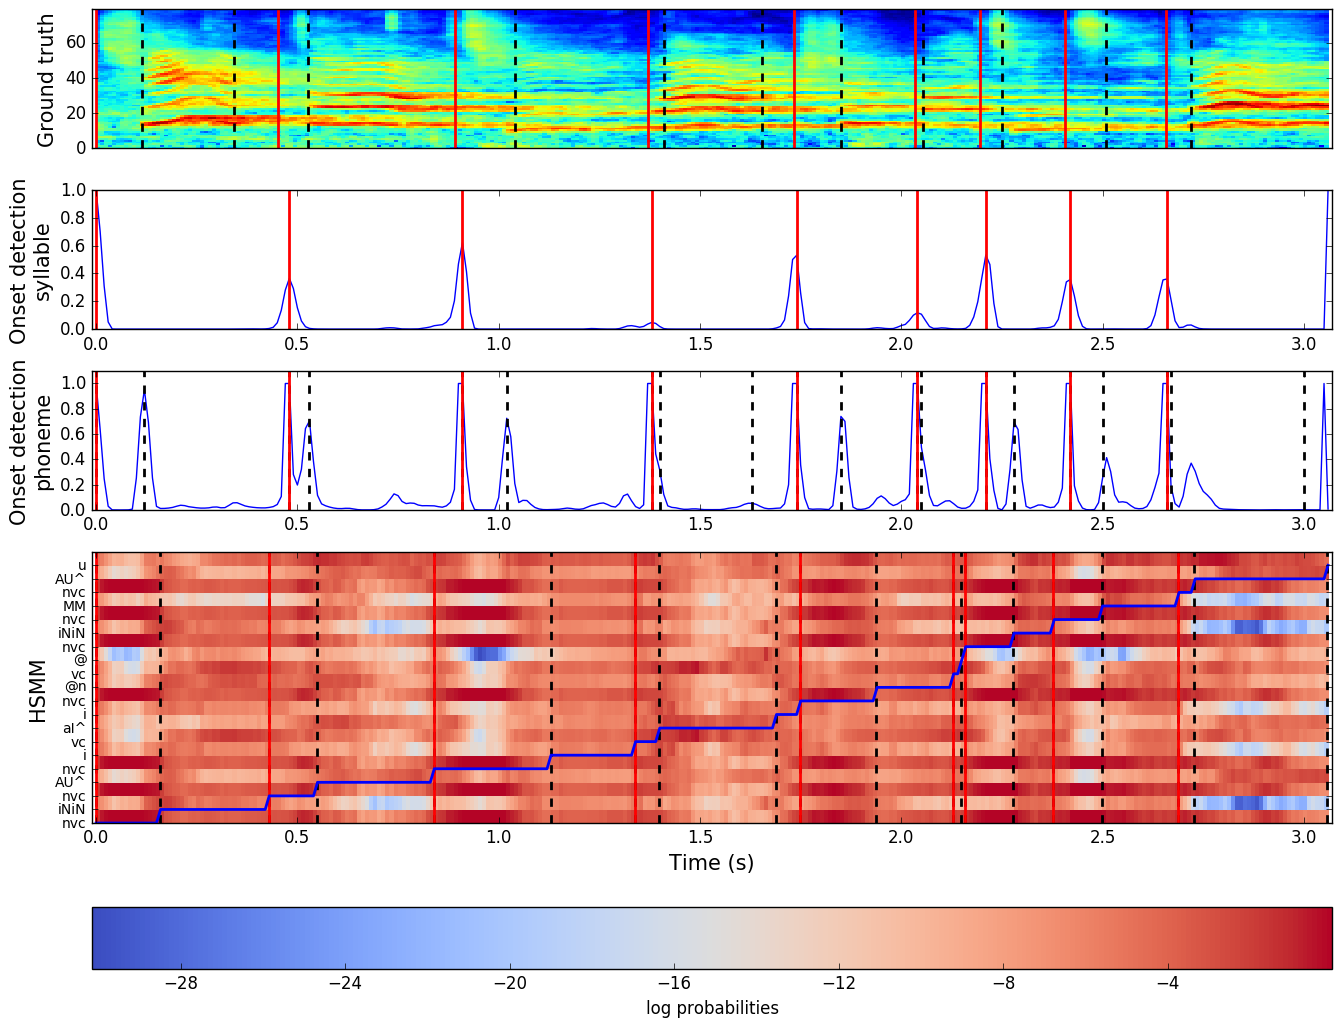
\includegraphics[width=\textwidth]{figs/results/ch5_results_segmentation.png}
    \caption{An illustration of the result for a singing phrase in the testing part of the dataset. The red solid and black dash vertical lines are respectively the syllable and phoneme onset positions. 1st row: ground truth, 2nd and 3rd rows: onset detection-based method, 4th row: HSMM-based segmentation method. The blue curves in the 2nd and 3rd row are respectively the syllable and phoneme ODFs. The staircase-shaped curve in the 2nd row is the alignment path.}
    \label{fig:ch5:results_example_onset}
\end{figure}

Fig \ref{fig:ch5:results_example_onset} shows an result example for a singing phrase in the testing part of the dataset. Notice that there are some extra or missing onsets in the detection. This is due to the inconsistency between the coarse duration input and the ground truth, for example, students might sing extra or miss some phonemes in the actual singing. Also notice that in the 3rd row, the two detected phoneme onsets within the last syllable are not in the peak positions of the ODF. This is due to that the onsets is inferred by taking into account both ODF and the \textit{a priori} duration model, and the latter partially constraints the detected onsets.

The biggest advantage of the proposed method is the language-independency, which means that the pre-trained CNN model can be eventually applied to the singing voice of various languages because they could share the similar temporal-spectral patterns of phoneme transitions. Besides, the Viterbi decoding of the proposed method (time complexity $O(TS^2$), $T$: time, $S$: states) is much faster than the HSMM counterpart (time complexity $O(TS^2+T^2S)$). To showcase the proposed algorithm, an interactive jupyter notebook demo is provided for running in Google Colab\footnote{\url{https://goo.gl/BzajRy}}. 

\section{Improving the deep learning-based onset detection model}

In the last section, we devised an onset detection-based syllable and phoneme segmentation method which firstly estimates the onset detection function (ODF) by using a deep learning classification model, then selects the correct onsets on the ODF by using a duration-informed HMM model. It is obvious that the accuracy of the onset selection step depends on largely on the quality of the ODF. Thus, it is necessary to explore an effective and efficient deep learning architecture for estimating the ODF.

In this section, we experiment with seven deep learning architectures for estimating syllable onset detection functions to find the most effective and efficient one for the onset detection task. The seven deep learning models are compared and evaluated on a jingju a cappella singing test dataset presented in \secref{sec:ch4:dataset_segmentation}.

\subsection{Deep learning onset detection functions}\label{sec:ch5:nn_onset_improving}

We introduce the neural network setups and training strategies for the experiment which aims to find the most efficient network architecture trained separately on a jingju singing test dataset for syllable onset detection.

\subsubsection{Searching for the most efficient neural network architecture}\label{sec:ch5:architectures_improving}

Following the terminology used in Pons et al.'s work\cite{Pons2017}, we regard a neural network architecture as two parts -- front-end and back-end. According to their work, the front-end is the part of the architecture which processes the input features and maps it into a learned representation. The back-end predicts the output given the learned representation. In this research, we don't restrict the functionality of back-end to prediction. However, we use it as terminology to differentiate from the front-end. We present the front-ends in table \ref{table:frond_ends} and back-ends in table \ref{table:back_ends}. \textbf{Conv} means convolutional layer. \textbf{10x} $\boldsymbol{3\times7}$ means 10 filters of which each convolves on 3 frequency bins and 7 temporal frames. All the Conv layers use ReLU activations. The first Conv layer in the front-end B has 6 different filter shapes. Each Conv layer in back-end C and D follows by a batch normalization layer to accelerate the training\cite{Ioffe2015}. \textbf{BiLSTMs} means bidirectional RNN layers with LSTM units. In back-end B, both forward and backward layers in BiLSTMs have 30 units with Tanh activations. The activation function type of \textbf{Dense} layer -- ReLU or Sigmoid used in back-end A depends on the architecture.

\begin{table}[ht!]
\centering
\caption{Architecture front-ends}
\label{table:frond_ends}
\begin{tabular}{c|c}
\toprule
Front-end A & Front-end B \\
\midrule
Conv 10x $3{\times}7$ & \makecell{Conv 24x $1{\times}7$, 12x $3{\times}7$, 6x $5{\times}7$\\24x $1{\times}12$, 12x $3{\times}12$, 6x $5{\times}12$} \\
Max-pooling $3{\times}1$ & Max-pooling $5{\times}1$ \\
Conv 20x $3{\times}3$ & Conv 20x $3{\times}3$ \\
Max-pooling $3{\times}1$ & Max-pooling $3{\times}1$\\
Dropout 0.5 & Dropout 0.5\\
\bottomrule

\end{tabular}
\end{table}

\begin{table}[ht!]
\centering
\caption{Architecture back-ends}
\label{table:back_ends}
\begin{tabular}{c|c}
\toprule
Back-end A  & Back-end B    \\
\midrule
Dense 256 units & Flatten \\
Flatten & BiLSTMs 30 units \\
Dropout 0.5 & Dropout 0.5\\
% \bottomrule     

\toprule
Back-end C  & Back-end D    \\
\midrule
Conv 40x $3{\times}3$ & Conv 60x $3{\times}3$ \\
Conv 40x $3{\times}3$ & Conv 60x $3{\times}3$ \\
Conv 40x $3{\times}3$ & Conv 60x $3{\times}3$ \\
Conv 80x $3{\times}3$ & Flatten \\
Conv 80x $3{\times}3$ & Dropout 0.5 \\
Conv 80x $3{\times}3$ & \\
Conv 135x $3{\times}3$ & \\
Flatten & \\
Dropout 0.5 & \\
\bottomrule
\end{tabular}
\end{table}

We present seven architectures which are the combination pipelines of the front-ends and back-ends. All back-ends are connected with a sigmoid unit to output the ODF for the input log-mel contexts.

\noindent\textbf{Baseline}: Front-end A + back-end A with sigmoid activations. This architecture is the same as the one described in Schl\"{u}ter and B\"{o}ck's work \cite{Schluter2014}.

\noindent\textbf{ReLU dense}: Front-end A + back-end A with ReLU activations. In Schl\"{u}ter and B\"{o}ck's work \cite{Schluter2014}, using ReLU activations in the back-end A caused a drop in performance when evaluating on B\"{o}ck dataset. However, ReLU activation function has been shown to enable better training of deeper networks because it has several advantages compared with Sigmoid, such as reducing the likelihood of vanishing gradient \cite{Glorot2011}. We want to (re-)test the performance of ReLU activation on both B\"{o}ck and jingju dataset.

\noindent\textbf{No dense}: Front-end A + Flatten layer. We use this architecture to test the effect of removing the dense layer in the baseline.

\noindent\textbf{Temporal}: Front-end B + back-end A with sigmoid activations. This one is similar to the ``Temporal architecture'' presented in Pons et al.'s work \cite{Pons2017}, and uses various filter shapes in the first convolutional layer. In this work, we use 6 different filter shapes which are wide in temporal axis and narrow in frequency axis. Such kind of filter shape design aims to capture the onset spectral-temporal patterns on the spectrogram. It has been shown experimentally that on a smaller jingju dataset, this architecture outperformed the baseline by effectively learning the temporal onset patterns.

\noindent\textbf{BiLSTMs}: Front-end A with time-distributed Conv layers + back-end B. This one is similar to the CRNNs architectures presented in Vogl et al.'s work \cite{Vogl2017DrumTV}. We use the sequence of the log-mel contexts as the architecture input and we experiment 3 different sequence lengths -- 100, 200 and 400 frames. At the training phase, two consecutive input sequences are overlapped but their starting points are distanced by 10 frames. At the testing phase, the consecutive input sequences are not overlapped. We use this architecture to test the effect of replacing the dense layer in the baseline by RNN layer.

\noindent\textbf{9-layers CNN}: Front-end A + back-end C. We use this architecture to test the performance of deep CNN without using dense layer.

\noindent\textbf{5-layers CNN}: Front-end A + back-end D. As our datasets are relatively small, the above 9-layers CNN could be overfitting. Thus, we test also this shallow architecture with 5 CNN layers.

\begin{table}[ht!]
\centering
\caption{Total numbers of trainable parameters (TNoTP) of each architecture.}
\label{table:parameters}
\resizebox{\columnwidth}{!}{
\begin{tabular}{cccc}
\toprule
Baseline   & ReLU dense   & No dense     & Temporal \\
\midrule
289,273    & 289,273      & 3,161        & 283,687  \\
\toprule
BiLSTMs & 9-layers CNN & 5-layers CNN &          \\
\midrule
278,341    & 288,286      & 81,541       &      \\
\bottomrule
\end{tabular}
}
\end{table}

The Total numbers of trainable parameters (TNoTP) of each architecture is shown in table \ref{table:parameters}. To keep a fair comparison, we maintain a similar TNoTP between the baseline, ReLU dense, Temporal, BiLSTMs and 9-layers CNN architectures. We reduce the parameter numbers in No dense and 5-layers CNN architectures to explore the model efficiency. Notice that 9-layers and 5-layers CNNs are not fully-convolutional architectures \cite{Long2015} since we don't perform average pooling to the last Conv layer.

\subsubsection{Model training}\label{sec:ch5:model_training_improving}

We use the same target label preparing strategy been described in Schl\"{u}ter and b\"{o}ck's work \cite{Schluter2014}. The target labels of the training set are prepared according to the ground truth annotations. We set the label of a certain context to 1 if an onset has been annotated for its corresponding frame, otherwise 0. To compensate the human annotation inaccuracy and to augment the positive sample size, we also set the labels of the two neighbor contexts to 1. However, the importance of the neighbor contexts should not be equal to their center context. Thus the sample weights of the neighbor contexts are compensated by being set to 0.25. The labels are used as the training targets in the deep learning models to predict the onset presence.

Binary cross-entropy is used as the loss function. The model parameters are learned with mini-batch training (batch size 256), Adam \cite{kingma2014adam} update rule. 10\% training data is separated in a stratified way for early stopping -- if validation loss is not decreasing after 15 epochs. In all experiments, we use \texttt{Keras}\footnote{\url{https://github.com/keras-team/keras}} with \texttt{Tensorflow}\footnote{\url{https://github.com/tensorflow/tensorflow}} backend to train the models.

\subsection{Onset selection}\label{sec:ch5:onset_selection_improving}
The ODF output from the model is smoothed by convoluting with a 5 frames Hamming window. Onsets are then selected on the smoothed ODF. Two onset selection methods are evaluated.  The first is a peak picking method which has been used in many MOD works \cite{Bock2012c, Schluter2014,Vogl2017DrumTV}. We use the \texttt{OnsetPeakPickingProcessor} module implemented in \textsc{Madmom} \cite{Bock2016} package. Please refer to our code for its detailed parameter setting. Another onset selection method is based on the score-informed HMM presented in \secref{sec:ch5:dur_label}, which has been used to take advantage of the prior syllable duration information of the musical score.

\subsection{Experimental setup}\label{sec:ch5:eval_improving} 

We use ASPS\textsubscript{2} test dataset presented in \secref{sec:ch4:dataset_segmentation} and the metric -- onset detection accuracy presented in \secref{sec:ch2:evaluation_metrics} to evaluate the performance of each algorithms. We report the evaluation results for both peak-picking and score-informed HMM onset selection methods on jingju dataset. The pick-peaking results are reported by grid searching the best threshold on the test set, and the score-informed HMM results are evaluated directly on the test set since no optimization is needed.

We report only F1-measure in this paper. 
%Other metrics -- precision and recall can be consulted on the Github page\footnote{\url{https://github.com/musicalOnset-ismir2018/musicalOnset-ismir2018}\label{fn:github}}. 
For jingju dataset, to average out the network random initialization effect, each model is trained 5 times with different random seeds, then the average and standard deviation results are reported. To measure the statistical significance of the performance improvement or deterioration, we calculate the Welch's t-test on the 5 training times results for jingju dataset. We report two tails p-value and reject the null hypothesis if the p-value is smaller than 0.05.

\subsection{Results and discussions}

In this section, we report and analyze the results for the most efficient architecture searching experiments. In tables \ref{table:peak_picking_jingju_archi}, the p-value is calculated by comparing each model results with \textbf{Baseline}.

\begin{table}[ht!]
\centering
\caption{Jingju dataset peak-picking (upper) and score-informed HMM (bottom) results of different architectures.}
\label{table:peak_picking_jingju_archi}
\begin{tabular}{l|cc}
\toprule
               & F1-measure & p-value \\
\midrule
Baseline     &76.17$\pm$0.77     & -- \\
ReLU dense     &76.04$\pm$1.02       & 0.840              \\
No dense       &73.88$\pm$0.44       & 0.002              \\
Temporal       &76.01$\pm$0.61       & 0.749              \\
BiLSTMs 100 &78.24$\pm$0.83       & 0.006              \\
BiLSTMs 200 &77.82$\pm$0.68       & 0.013              \\
BiLSTMs 400 &76.93$\pm$0.68       & 0.178              \\
9-layers CNN   &73.83$\pm$0.92        & 0.005              \\
5-layers CNN   &76.68$\pm$1.04         & 0.457             \\
% \bottomrule
% \end{tabular}
% \end{table}

% \begin{table}[ht!]
% \centering
% \caption{Jingju dataset score-informed HMM results.}
% \label{table:score_informed_jingju_archi}
% \begin{tabular}{l|cc}
\toprule
               & F1-measure & p-value \\
\midrule
Baseline     & 83.23$\pm$0.57     & --        \\  
ReLU dense     & 82.49$\pm$0.28        & 0.057              \\
No dense       & 82.19$\pm$0.44         & 0.021              \\
Temporal       & 83.23$\pm$0.57         & 1                  \\
BiLSTMs 100 & 82.99$\pm$0.31         & 0.479              \\
BiLSTMs 200 & 83.29$\pm$0.37         & 0.882              \\
BiLSTMs 400 & 82.47$\pm$0.54        & 0.087              \\
9-layers CNN   & 80.90$\pm$0.67         & 0.001              \\
5-layers CNN   & 83.01$\pm$0.76        & 0.649             \\
\bottomrule
\end{tabular}
\end{table}

Observing table \ref{table:peak_picking_jingju_archi} -- the results of jingju dataset, \textbf{BiLSTMs 100} and \textbf{200} outperform \textbf{Baseline} with peak-picking onset selection method but not with score-informed HMM method. \textbf{9-layers CNN} overfits and significantly performs worse than \textbf{Baseline}, which means this architecture is too ``deep" and overfitted for this test dataset (check the Github page\footnotemark[\getrefnumber{fn:github}] for its loss curve). \textbf{Temporal} architecture has the p-value of 1 when evaluating by score-informed HMM method, and we confirm that it is a coincidence after having checked its 5 training times F1-measures. \textbf{No dense} architecture performs significantly worse than \textbf{Baseline}. However, considering its tiny TNoTP -- 3,161, this performance is quite acceptable. The similar case has been reported in Lacoste and Eck's work\cite{Lacoste2007a}, where their 1 unit 1 hidden layer architecture achieved a remarkable result (only 4\% F1-measure worse than their best architecture). This means that if the state-of-the-art performance is not required, one can use a quite small and efficient architecture. The score-informed HMM onset selection method outperform the peak-picking by a large margin. Also notice that the score-informed HMM method is able to compensate both good and bad performance of peak-picking, which can be seen by comparing upper and bottom results regarding \textbf{No dense}, \textbf{BiLSTMs 100} and \textbf{200} models.

Finally, we choose \textbf{5-layers CNN} as the most efficient architecture because it performs consistently equivalent to \textbf{Baseline} but only contains 28.3\% TNoTP. Although \textbf{Temporal} architecture performs equally well, it is not selected because its equal TNoTP to \textbf{Baseline} and the complex configuration of its front-end B. \textbf{BiLSTMs} outperforms \textbf{Baseline} on jingju dataset, however, due to its overfitting on B\"{o}ck dataset and slow training, we don't consider it as an efficient architecture.

Experiment code
%full results (precision, recall and F1-measure) 
and pre-trained models used in the experiments are available in Github\footnotemark[\getrefnumber{fn:github}]. A Jupyter notebook is prepared for showcasing the performance of different network architectures\footnote{\url{https://goo.gl/Y5KAFC}}. 

\section{Conclusions}

We formulate the syllable and phoneme segmentation problem within the context of jingju singing from two different perspectives -- lyrics-to-audio alignment and onset detection. After setting up the baseline HSMM-based segmentation (alignment) method, we proposed the duration-informed onset detection-based method for tackling the segmentation problem. Finally, we explored various deep learning architectures for improving the syllable onset detection performance.

A detailed evaluation of HSMM-based segmentation method, onset detection-based method and various deep learning onset detection models was discussed for two jingju a cappella singing test datasets. Jingju singing, with distinct musical characteristics, is an ideal case to study the performance of novel methods for syllable and phoneme segmentation.

The duration-informed onset detection-based method explicitly considered coarse syllable and phoneme duration information for the segmentation. However, the algorithm is language-independent, and thus can easily adapt to the singing voice of various languages and even to instrumental playing. Since onset detection-based method is a binary onset/non-onset classification model, it requires a small amount of syllable or phoneme onset annotated training data.

The duration-informed onset detection-based method shows significant promise in syllable and phoneme segmentation task. It provides a significant improvement in both onset detection and segmentation performance compared with the baseline HSMM-based method for jingju a cappella singing. An exploration of various deep learning syllable onset detection models showed that the architecture of the deep learning model cannot affect significantly the onset detection performance, however, one can design an efficient architecture to reach the state of the art performance.

One main limitation of the onset detection-based method presented was the assumption that a similar duration of each syllable or phoneme and the same syllable or phoneme sequence should be sung between teacher's and student's singing pieces. While this is a fair and realistic assumption for jingju professional training since the students can usually imitate the teacher's singing very well, amateur singers might imitate very badly because of a large deviation of the syllable or phoneme duration and missing or extra syllable or phoneme. A coarse syllable and phoneme duration correction might be necessary there before applying the segmentation algorithm. The syllable or phoneme recognition might be the method used to tackle the problem of missing or extra syllable in student's singing.

The onset detection-based segmentation method utilized duration-informed HMM to select the correct onsets on the onset detection function (ODF). A good quality ODF is essential to reach a desirable syllable or phoneme onset detection/segmentation accuracy. Various deep learning architectures were experimented to search for a most effective and efficient one which can lead to a superior syllable onset detection performance. Although the experiment did not show an improvement in onset detection accuracy, we witnessed that a CNN architecture without dense connection reached the state of the art performance, while it has much less trainable parameters than the baseline architecture, which indicates that the segmentation model efficiency can be improved by using this deep learning architecture.

The presented onset detection-based segmentation method can be further improved to incorporate other linguistic information such as the phoneme class of each time frame. This is in addition to the ideas explored already -- HSMM-based method utilized phoneme class and duration information, while onset detection-based method utilized syllable/phoneme onset and duration information. Such a model which makes use of all of the three information -- onset, phoneme class and duration need to be further explored.

The automatic syllable and phoneme segmentation methods discussed in the chapter are aligned with the goal to lead towards an automatic pronunciation assessment system in a fine granularity for jingju a cappella singing. Syllable and phoneme segmentation is the first step towards this goal. The methods of mispronunciation detection and pronunciation similarity measures are built based on the results of the segmentation.

%\chapter{Percussion pattern transcription and discovery}\label{chap:percpatt}
\begin{epigraphs}
  \qitem{The metaphorical usage of `language' for a musical system is paralleled by a literal usage that refers to the ways in which many drum musics may be represented with spoken syllables.}{\citeA{kippen:89:perclanguage}}
\end{epigraphs}
%\textit{Chapter in brief: Present the second thesis problem of percussion pattern discovery. This chapter presents preliminary work in percussion pattern transcription as applied to both CM and HM, with a special emphasis on methodology but less so on results. Beijing Opera is used as a -test case before applying on CM and HM. The chapter is short and shallow - include mainly for completeness. The material comes from ICASSP 2014, ISMIR 2014, ISMIR 2015 papers and unpublished results so far.}
% \update{TODO: Intro to be cleaned up}
\noindent Percussion plays an important role in Indian art music with a significant freedom to improvise, leading a wide variety of percussion patterns that help to create multiple layers of rhythm. An analysis of these percussion patterns hence is an important step towards developing rhythm similarity measures. We wish to discover percussion patterns from audio recordings in a data-driven way, while using a musically meaningful representation for percussion patterns. 

We address the task of percussion pattern \index{Percussion pattern}discovery in this chapter taking an approach of transcription followed by a search for patterns. The work presented in the chapter is basic and exploratory, and only for demonstrating the utility of a syllabic percussion system in percussion pattern transcription and discovery. Most experiments presented contain preliminary results, needing further work. The goals of the chapter are: 
\begin{enumerate}[leftmargin=*]
 \item To discuss two broad approaches to percussion transcription. To focus on timbre based transcription, and to present how meaningful representations can be obtained for overall timbres of percussion strokes in syllabic percussion systems.
 \item To present an approach to percussion pattern transcription and discovery in syllabic percussion systems based on a speech recognition framework.
 \item To present experiments on \gls{jingju} percussion patterns, as a simpler example test case of percussion pattern transcription and pattern classification. To extend the approach to Indian art music, and evaluate it on mridangam and tabla solo datasets. 
 \item To identify the advantages and shortcomings of such an approach, with possible future research directions to pursue. 
\end{enumerate}
We first start by describing two broad approaches that can be taken for the task of percussion pattern transcription. 
%
\section{Approaches} %  to percussion pattern transcription and discovery
% \note{Two approaches - onset detection + instrument ID, or combined. But this does not make use of the syllabic structure, and hence we have the new method based on speech recognition.}
Percussion transcription aims to transcribe an audio recording of a percussion solo into a time aligned sequence of symbols. Depending on the symbol set chosen and the acoustic events being modeled, transcription can be approached in two different broad ways. The two approaches differ mainly in the way they define percussion patterns in audio. % and transcribe and discover 
\subsubsection{Transcription based on individual instruments}
An audio recording can be transcribed into time aligned sequence of individual percussion instrument stroke onsets, e.g. transcribing a drum solo into a sequence of bass, hi-hats and snare drum onsets. The output of such a task is a drum score showing all the drums, and their onset times. A percussion pattern can then be described and represented using that score, using the onset information from all instruments. Such an approach is useful for transcription from drum mixtures, when percussion patterns are defined as a sequential combination of different instruments, each retaining their own musical identity. Since most percussion solos have simultaneous strokes from multiple instruments, such an approach needs a decomposition of the audio containing drum mixtures into individual drum components. As a pre-processing step, an instrument-wise onset detection might be needed. 

As discussed before in \secref{sec:bkgnd:sotapercpatt}, event-based transcription algorithms~\cite{gillet:04:drumloops,gouyon:02:pulse,goto:94:soundSep,gillet:08:transcription} segment the input signal based on percussion events then extract and classify features from these segments to uncover its musically meaningful content, such as onsets. Source separation based methods~\cite{paulus:05:drum,smaragdis:04:convNMF,abdallah:03:probability} decompose the input audio signal containing drum mixtures into basis functions capturing spectral characteristics of the sources (ideally, individual percussion instruments). \citeA{tian:14:icassp} present an exploratory study on the use of \gls{NMF} based source separation techniques for instrument specific onset detection in \gls{jingju} percussion instrument ensembles, aiming at providing a baseline for further research in \gls{jingju} percussion transcription. 
%
\subsubsection{Transcription based on overall timbre}
A contrasting approach is to consider the overall timbre sequence of a percussion solo, without any regard to individual instruments. A percussion pattern is then defined as a sequence of combined instrument timbres and the goal is to transcribe an audio recording into a sequence of such combined timbres. Such an approach is useful when percussion patterns can be defined based on timbral sequences e.g. in syllabic percussion systems. A notable limitation of the approach however is when a pattern cannot be accurately defined by the overall timbre, and individual instrument timbres are necessary, as often is the case with a drum set. 

In syllabic percussion\index{Syllabic percussion} systems, patterns can be defined using syllables, which is both musically meaningful and accurate in representation. In certain percussion systems such as in \gls{jingju} percussion, the syllables represent the overall combined timbre of a percussion ensemble, while in Indian art music (both Carnatic and Hindustani music), the syllables represent the different timbres that can be produced by the (often) single percussion instrument used, either the \gls{tabla} or the mridangam. In either case, the overall timbre represented by the syllable is sufficient to define a percussion pattern. In such a case, a percussion pattern can be represented solely based on these syllables and transcribed as such. 

In this chapter, we explore only the second approach, using syllables to define overall timbres of percussion strokes. We then use them to define, transcribe and discover percussion patterns. In the remainder of the chapter, the goal is to test the effectiveness and relevance of percussion syllables in representation and modeling of percussion patterns for automatic transcription and discovery. Since these syllables have a clear analogy to speech and language, the transcription task has a definite analogy to speech recognition and we can apply several tools and knowledge from this well explored research area with many state of the art algorithms and systems~\cite{huang:10:sroverview}. 

The final goal is to automatically discover percussion patterns from segmented percussion solo audio recordings of Indian art music, and we take a transcription + search approach as briefly discussed in \secref{sec:probdef:thesispattern}. The task however is challenging since it requires a concrete definition of a percussion pattern, while such a definition of what constitutes a percussion pattern is ambiguous in Indian art music. Further, Indian percussion has a great scope for improvisation within the framework of the \gls{tala}. This leads a large number of percussion patterns that can be played on the mridangam and tabla, which makes it further difficult to define relevant percussion patterns without ambiguity. We address this issue by making the discovery unsupervised and data-driven, by using transcribed ground truth music scores to define relevant patterns. 

Given the complexity of the task in Indian art music due to ill-defined large number of patterns, we consider the case of percussion patterns in \gls{jingju} as an initial test case for our hypothesis and methods. Percussion patterns in \gls{jingju} are simpler in both these aspects when compared to Indian art music: \gls{jingju} percussion patterns are well defined and limited in number. Once we demonstrate and validate our hypothesis with \gls{jingju}, we extend the methodology to Indian art music, with a data-driven but extendable definition of a percussion pattern. Since there are a limited number of \gls{jingju} percussion patterns, the problem of pattern discovery in \gls{jingju} is simplified into a pattern classification task, as is described further in the following section. 
%
\section[The case of Beijing opera]{The case of Beijing opera (\Gls{jingju})}\label{sec:ppclassify:jingju}
\begin{figure}
\captionsetup[subfigure]{labelformat=empty}
\centering
\subfloat[]{\label{fig:boperc:instwav} 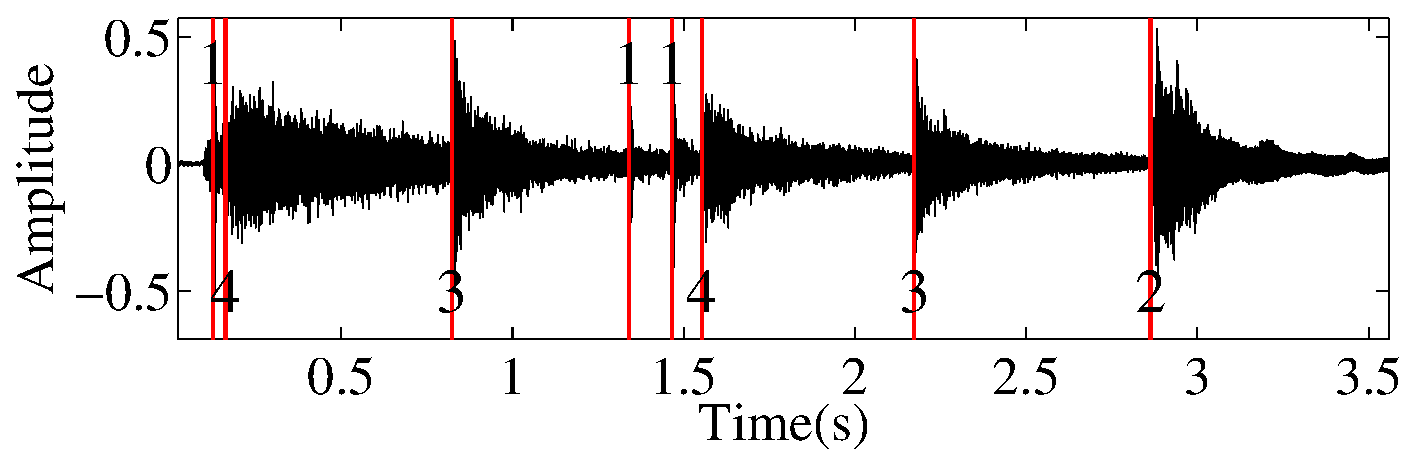
\includegraphics[width=0.95\textwidth]{jingjuPatts/jingju-stroke-waveform.pdf}}\\ \vspace{-1cm} 
\subfloat[]{\label{fig:boperc:instspec} \hspace{1.2mm} \includegraphics[width=0.93\textwidth]{jingjuPatts/jingju-stroke-spectrum.pdf}} 
\caption[Waveform and spectrogram of \gls{jingju} percussion strokes]{The waveform and spectrogram of an audio example containing all four instrument groups of \gls{jingju}. The top panel shows the waveform and the bottom panel is the spectrogram, the x-axis for both panels is time (in seconds). The vertical lines (in red) mark the onsets of the instruments. The onsets are labeled to indicate the specific instruments: \gls{bangu}-1, \gls{daluo}-2, \gls{naobo}-3, \gls{xiaoluo}-4.}\label{fig:bo:instwavspec}
\end{figure}
To recall from \secref{sec:bkgnd:bopercussion}, percussion ensemble in \gls{jingju} consists of five instruments played by four musicians, and can be grouped based on timbre into four instrument groups - \gls{bangu} (clapper-drum), \gls{xiaoluo} (small gong), \gls{daluo} (big gong) and \gls{naobo} (cymbals). The waveform and spectrogram of an audio example with all four of these instrument classes is shown in \figref{fig:bo:instwavspec}\footnote{The audio example is available here: \url{http://www.freesound.org/people/ajaysm/sounds/205971/}}. We can see the amplitude dynamics and spectral shapes for each instrument. \Gls{daluo} has a falling pitch, while \gls{xiaoluo} has a rising pitch profile. \Gls{naobo} has a broadband spectrum with significant energy in higher frequencies, as is characteristic of cymbals. Onsets generated by \gls{bangu} are sharp, have a much lower amplitude and shorter transient time, and happen in higher density than those generated by the other instruments. Hence, the \gls{bangu} onsets are easily masked by the cymbals and gongs. We can also see how the \gls{bangu} stroke is masked by an adjoining \gls{xiaoluo} stroke (0-0.5s in \figref{fig:bo:instwavspec}).

Using combinations of these instruments, several different combined percussion strokes are produced, each of which is labeled with an onomatopoeic oral mnemonic syllable\index{Oral mnemonic syllable}. Since there are many syllables that map to a single timbre, we reduced the complete set of syllables into five syllable groups - \syl{DA}, \syl{TAI}, \syl{QI}, \syl{QIE}, and \syl{CANG}, as listed in \tabref{tab:bo:sylmap}. The use of these oral syllabic sequences simplify and unify the representation of these patterns played by an ensemble. 

To further recall \secref{sec:bkgnd:bopercussion}, the percussion patterns in \gls{jingju} music are sequences of strokes played by different combinations of the percussion instruments, and the resulting variety of timbres are transmitted using oral syllables as mnemonics. Each percussion pattern is a sequence of syllables in their pre-established order, along with their specific rhythmic structure and dynamic features. Each particular pattern has a single unique syllabic representation shared by all the performers. Hence, the use of these oral syllabic sequences simplify and unify the representation of these patterns played by an ensemble, making them optimal for the transcription and automatic classification of the patterns.
\begin{figure}
\captionsetup[subfigure]{labelformat=empty}
\centering
\subfloat[]{\label{bowaveform} \includegraphics[scale=0.4]{percPatterns/waveform-shanchui.pdf}}\\ \vspace{-1cm}
\subfloat[]{\label{bospectrum} \hspace{-0.9mm} \includegraphics[scale=0.4]{percPatterns/spectrum-shanchui.pdf}}
\caption[Waveform and spectrogram of the pattern \gls{shanchui}]{The waveform and spectrogram of an audio example of the pattern \gls{shanchui}. The top panel shows the waveform and the bottom panel is the spectrogram. The vertical lines (in red) mark the onsets of the syllables. The onsets are labeled to indicate the specific syllable group: \syl{DA}-1, \syl{TAI}-2, \syl{QI}-3, \syl{QIE}-4, and \syl{CANG}-5 (\syl{QI} is not present in this pattern). The score for the pattern is shown in \protect\figref{fig:bopatt:shanchui}. Notice that the audio example has two additional repetitions of the sub-sequence \syl{CANG}-\syl{TAI}-\syl{QIE}-\syl{TAI} in the pattern.}\label{fig:bopercpatt:audio}
\end{figure}

A performance starts and ends with percussion patterns, they generally introduce and conclude arias, and mark transition points within them. The patterns accompany the actors' movements on stage and set the mood of the play, the scene, the aria or a section of the aria. An automatic description of these percussion patterns is thus quite important in providing the overall description of the aria. Therefore, the detection and characterization of percussion patterns is a fundamental task for the description of the music dimension in Beijing opera. In practice, there is a limited set of named patterns that are played in performance. 

Though the patterns are limited in number and predefined, there are several challenges to the problem of percussion pattern transcription and classification. Being an oral tradition, the syllables used for the representation of the patterns lack full consistency and general agreement. The result being that one particular timbre might be represented by more than one syllable. Furthermore, the syllabic representation conveys information for the conjoint timbre of the ensemble, so only the main structural sounds are represented. In an actual performance, a particular syllable might be performed by different combinations of instruments - e.g. in \figref{fig:bopatt:shanchui}, the first occurrence of the syllable \syl{TAI} is played just by the \gls{xiaoluo}, but in the rest of the pattern is played by \gls{xiaoluo} and the \gls{bangu} together. In fact, generally speaking, the strokes of the \gls{bangu} are seldom conveyed in the syllabic sequence (as can be seen in the third measure in \figref{fig:bopatt:shanchui} for the second sixteenth-note of the \gls{bangu}), except for the introductions and other structural points played by the drum alone. As indicated in \tabref{tab:bo:sylmap}, \syl{CANG} is mostly a combination of all the three metallophones, but in some cases, \syl{CANG} can be played with just the \gls{daluo}, or just the \gls{daluo}+\gls{naobo} combination. 

In the cases where the percussion pattern is to accompany the movements of actors on stage, certain syllable subsequences in the pattern are repeated indefinitely. This causes the same pattern in different performances to have variable lengths, and these repetitions need to be explicitly handled. The timing of these patterns is expressive and matches the acting in the scene, and hence we consider only the sequence of syllables and do not consider timing relationships between the syllables to define patterns. Finally, although the patterns are usually played in isolation, in many cases the string instruments or even the vocals can start playing before the patterns end, presenting challenges in identification and classification. \figref{fig:bopercpatt:audio} shows an audio example of the pattern \gls{shanchui}, along with time aligned markers to indicate the syllable onsets. The spectrogram also shows the timbral characteristics of the percussion instruments \gls{xiaoluo} (increasing pitch) and \gls{daluo} (decreasing pitch). Some variation to the notated score can also be seen, such as expressive timing and additional insertion of syllables.

At the outset, it is clear that Beijing opera percussion patterns are well defined and limited in number. Further, in \gls{jingju}, the recognition of the pattern as a whole is more important than an accurate syllabic transcription of the pattern. Due to the limited set of pattern classes and owing to all the variations possible in a pattern, we are primarily interested in classifying an audio pattern into one of the possible pattern classes. Syllabic transcription is only considered as an intermediate step towards pattern classification. The named patterns can be used to build a library of patterns. The patterns can be referred to as ``pattern classes" for the purpose of classification, and classifying an instance of a pattern occurring in the audio recording of an aria into one of these pattern classes is thus a primary task. 
% 
\subsection{Percussion pattern classification}
Beijing opera percussion pattern transcription and classification is a first test case for percussion pattern discovery approaches. In this work, we restrict to five predominantly used percussion patterns in \gls{jingju} - \gls{daobantou}, \gls{manchangchui}, \gls{duotou}, \gls{xiaoduotou}, and \gls{shanchui} (pattern scores provided in \figref{fig:bopatt:scores}). Further, we restrict ourselves to percussion patterns that occur at the introduction of the aria, since they convey significant information about the structure of the aria that follows it, e.g. \gls{daobantou} pattern is followed by an aria in \gls{banshi} \gls{daoban}. %\comment{Check with Rafa, XX}  

We now present a formulation for transcription and recognition of syllable based audio percussion patterns, and evaluate it on the \acrfull{BOPP} (see \secref{sec:dataset:bopp}). The dataset is a collection of 133 audio percussion patterns spanning five different pattern classes, with over 2200 syllables in total. There is a significant analogy of this task to connected word speech recognition using word models. Syllables are analogous to words and a percussion pattern to a sentence - a sequence of words. There are language rules to form a sentence using a vocabulary, just as each percussion pattern is formed with a defined sequence of syllables from a vocabulary. However unlike in the case of speech recognition where infinitely many sentences are possible, in our case we have a small number of percussion patterns to be recognized.

Similar to the work by \citeA{nakano:04:voicePerc}, we explore a speech recognition based framework in this study. Their approach is different from ours in the sense that the onomatopoeic representations they used were created by the authors, while we are relying on already existing oral traditions. To the best of our knowledge, \citeA{ajay:14:ismirbo} presented the first work that explored automatic transcription and classification of syllable based percussion patterns, as applied to Beijing opera. The method and results presented in this section are from that work. 

Following the notation presented in \secref{sec:probdef:thesispattern}, consider a set of $\nPercPatterns$ pattern classes $\pattSet = \{\percPattSeq_1, \percPattSeq_2, \cdots \percPattSeq_\nPercPatterns\}$, each of which is a sequence of syllables from the set of syllables $\sylSet = \{\sylSetVar_1, \sylSetVar_2, \cdots \sylSetVar_\nSyllables\}$, where $\nSyllables$ is the total number of syllables in the set. Hence, a percussion pattern is represented as $\percPattSeq_i = [\sylVar_1, \sylVar_2, \cdots, \sylVar_{\pattLen_i}]$ where $\sylVar_j \in \sylSet$ and $\pattLen_i$ is the length of $\percPattSeq_i$. Given a test audio signal $\signal$ containing a percussion pattern, the transcription task aims to obtain a syllable sequence $\percPattSeq^{\optstar} = [\sylVar_1, \sylVar_2, \cdots, \sylVar_{\pattLen^{\optstar}}]$ and the classification task aims to assign $\percPattSeq^{\optstar}$ into one of the patterns in the set $\pattSet$. 

The syllables are non-stationary signals and to model their timbral dynamics, we build an \gls{HMM} for each syllable (analogous to a word-\gls{HMM}). Using these syllable \glspl{HMM} and a language model, an input audio pattern is transcribed into a sequence of syllables using Viterbi decoding\index{Viterbi decoding}, and then classified to a pattern class in the library using a measure of distance.
\begin{figure}[t]
\centering
 \includegraphics[width=\textwidth]{blockDiags/blockDiagJingjuPercClassify.pdf}
\caption[Block diagram: \Gls{jingju} percussion pattern classification]{The block diagram \gls{jingju} percussion pattern classification approach}\label{fig:BD:jingjuPercClassify}
\end{figure}

A block diagram of the approach is shown in \figref{fig:BD:jingjuPercClassify}. We first build syllable level \glspl{HMM} $\{\hmmSym_j\}$, $1 \leq j \leq \nSyllables (= 5)$, for each syllable $\sylSetVar_j$ using features extracted from the training audio patterns. We use the \gls{MFCC} features to model the timbre of the syllables. To capture the temporal dynamics of syllables, we add the velocity and the acceleration coefficients of the \gls{MFCC}. The stereo audio is converted to mono, since there is no additional information in stereo channels. The 13 dimensional (including the zeroth coefficient) \gls{MFCC} features are computed from audio patterns with a frame size of 23.2 ms and a shift of 5.8 ms. We also explore the use of energy (as measured by the zeroth \gls{MFCC} coefficient) in classification performance. Hence we have two sets of features, \acrshort{MFCCODA}, the 39 dimensional feature including the zeroth, delta (velocity) and double-delta (acceleration) coefficients, and \acrshort{MFCCDA}, the 36 dimensional vector without the zeroth coefficient. 

We model each syllable using a 5-state left-to-right \gls{HMM} including an entry and an exit non-emitting states. The emission densities for each state is modeled with a four component \gls{GMM} to capture the timbral variability in syllables. We experimented with eight and sixteen component \gls{GMM}, but with little performance improvement. Since we do not have time aligned transcriptions in the \acrshort{BOPP} dataset, an isolated \gls{HMM} training for each syllable is not possible. Hence we use an embedded model Baum-Welch re-estimation~\cite{huang:90:hmm} to train the \glspl{HMM} using just the syllable sequence corresponding to each feature sequence. The \glspl{HMM} are initialized with a flat start using all of the training data. All the experiments were done using the \acrfull{HTK} \cite{young:06:htkbook}. 

Given a test audio pattern, we use these syllable \glspl{HMM} to obtain a rough syllabic transcription and then classify the test pattern into one of the pattern classes in the library based on a measure of distance between the test pattern and the pattern classes. Since we only need a rough syllabic transcription independent of the pattern class, we treat the test audio pattern as a first order time-homogenous discrete Markov chain, which can consist of any finite length sequence of syllables, with uniform unigram and bigram (transition) probabilities, i.e. $P(\sylVar_1 = \sylSetVar_i) = 1/\nSyllables$ and $P(\sylVar_{k+1} = \sylSetVar_j \mid \sylVar_k = \sylSetVar_i) = 1/\nSyllables$, $ 1 \leq i,j \leq \nSyllables$, with $k$ being the sequence index. This also forms a simple uninformed language model\index{Language model} for forming the percussion patterns using syllables. Given a feature sequence extracted from test audio pattern, we use the \glspl{HMM} $\{\hmmSym_j\}$ to do a Viterbi (forced) alignment, which aims to provide the best sequence of syllables $\percPattSeq^{\optstar}$, given a syllable network constructed from the language model. 

Given the decoded syllable sequence $\percPattSeq^{\optstar}$, we compute the string edit distance \cite{navarro:01:strDist} between $\percPattSeq^{\optstar}$ and patterns in the set $\pattSet$. The use of edit distance is motivated by two factors. First, due to errors in Viterbi alignment, $\percPattSeq^{\optstar}$ can have insertions (\strInsErr), deletions (\strDelErr), substitutions (\strSubErr), and transposition (\strTrnErr) of syllables compared to the ground truth. Secondly, to handle the allowed variations in patterns, an edit distance is preferred over an exact match to the sequences in $\pattSet$. We explore the use of two different string edit distance measures, Levenshtein distance ($\distMeas_{1}$) that considers \strInsErr, \strDelErr, \strSubErr\ errors and the Damerau–Levenshtein distance ($\distMeas_2$) that considers \strInsErr, \strDelErr, \strSubErr, and also \strTrnErr\ errors~\cite{navarro:01:strDist}. 

As discussed earlier, there can be repetitions of a subsequence in some patterns. Though the number of repetitions is indefinite, we observed in the dataset that there are at most two repetitions in a majority of pattern instances. Hence for the pattern classes that allow repetition of a sub-sequence, we compute the edit distance for the cases of zero, one and two repetitions and then take the minimum distance obtained among the three cases. This way, we can handle repeated parts in a pattern. Finally, the $\percPattSeq^{\optstar}$ is assigned to the pattern class $\percPattSeq_o \in \pattSet$ for which the edit distance $\distMeas$ (either $\distMeas_1$ or $\distMeas_2$) is minimum, as in \eqnref{eqn:bo:pattclassify}.  
\begin{equation}
\percPattSeq_o = \underset{1 \leq j \leq \nPercPatterns}{\argmin}\;\distMeas(\percPattSeq^{\optstar},\percPattSeq_j) \label{eqn:bo:pattclassify}
\end{equation}
%
\subsection{Results and discussion}\label{sec:boperc:results}
We present the syllable transcription and pattern classification results on the \acrshort{BOPP} dataset described in \secref{sec:dataset:bopp}. The results shown in \tabref{tab:ppres:bopp} are the mean values in a leave-one-out cross validation. We report the syllable transcription performance using the measures of Correctness ($\corrMeas$) and Accuracy ($\accuMeas$). If $\pattLen$ is the length of the ground truth sequence, then the two measures are defined as,  
\begin{eqnarray}\label{eqn:pp:straccu}
\corrMeas & = & \frac{\pattLen - \strDelErr - \strSubErr}{\pattLen} \\
\accuMeas & = & \frac{\pattLen - \strDelErr - \strSubErr - \strInsErr}{\pattLen}
\end{eqnarray}
The Correctness measure penalizes deletions and substitutions, while Accuracy measure additionally penalizes insertions too. The pattern classification performance is shown for both edit distance measures $\distMeas_1$ and $\distMeas_2$ in \tabref{tab:ppres:bopp}. All the results are reported for both the features, \acrshort{MFCCODA} and \acrshort{MFCCDA}. The difference in performance between the two features was found to be statistically significant for both Correctness and Accuracy measures in a Mann-Whitney U test at $p = 0.05$, assuming an asymptotic normal distribution \cite{mann:47:Utest}.

In general, we see a good pattern classification performance despite a low syllable transcription accuracy. We see that the feature \acrshort{MFCCODA} leads to a better performance with syllable transcription, while both kinds of features provide a comparable performance for pattern classification. Though syllable transcription is not the primary task we focus on, an analysis of its performance provides several insights. The set of percussion instruments in Beijing opera is fixed, but there can be slight variations across different instruments of the same kind. The training examples are varied and representative, and models built can be presumed to be source independent. Nevertheless, there can be unrepresented syllable timbres in test data leading to a poorer transcription performance. A bigger training dataset can improve the performance in such a case. The energy (zeroth) co-efficient provides significant information about the kind of syllables and hence gives a better syllable transcription performance. 
\begin{table}
\centering
\begin{tabular}{@{}lcccccc@{}} \toprule
\multirow{2}{*}{Feature} & & \multicolumn{2}{c}{Syllable} & & \multicolumn{2}{c}{Pattern}\tabularnewline 
 & & $\corrMeas$ & $\accuMeas$ & & $\distMeas_1$ & $\distMeas_2$\tabularnewline \midrule
\acrshort{MFCCDA} & & 78.14 & 26.32 & & 93.23 & 89.47\tabularnewline 
\acrshort{MFCCODA} & & 84.98 & 39.63 & & 91.73 & 89.47\tabularnewline \bottomrule
\end{tabular}
\caption[Transcription and classification results on \acrshort{BOPP} dataset]{Syllable transcription and pattern classification performance on \acrshort{BOPP} dataset, with Correctness ($\corrMeas$) and Accuracy ($\accuMeas$) measures for syllable transcription. Pattern classification results are shown for both distance measures $\distMeas_1$ and $\distMeas_2$. All values are in percentage.} \label{tab:ppres:bopp}
\end{table}
%
\begin{table}
\centering
\begin{tabular}{@{}ll|cccccc@{}}\toprule
Pattern class & Total & ID & 1 & 2 & 3 & 4 & 5 \tabularnewline \midrule
\gls{daobantou} & 62 & 1 & 100 &  &  &  &  \tabularnewline 
\gls{manchangchui} & 33 & 2 & & 93.9 &  &  & 6.1 \tabularnewline 
\gls{duotou} & 19 & 3 &10.5 &  & 68.4 &  & 21.1 \tabularnewline 
\gls{xiaoduotou} & 11 & 4 & &  &  18.2 & 81.8 & \tabularnewline 
\gls{shanchui} & 8 & 5 & & 12.5 &  &  & 87.5 \tabularnewline \bottomrule
\end{tabular}
\caption[Confusion matrix for percussion pattern classification in \acrshort{BOPP} dataset]{The confusion matrix for pattern classification in \acrshort{BOPP} dataset, using the feature \acrshort{MFCCODA} with $\distMeas_1$ distance measure. The first and second column show the pattern class label and the total examples in each class, and class labels correspond to the ID in \tabref{tab:dataset:bopp}. The rows and column headers represent the True Class and Assigned Class, respectively. All other values are in percentage and the empty blocks are zeros (omitted for clarity).} \label{tab:ppres:boppconf}
\end{table}

We see that the Correctness is higher than Accuracy showing that the exact sequence of syllables, as indicated in the score was not achieved in a majority of the cases, with several insertion errors. This is due to the combined effect of errors in decoding and allowed variations in patterns. However, an edit distance based distance measure for classification is quite robust in the present five class problem and provides a good classification performance, despite the low transcription accuracy. 

Both distance measures provide comparable performance, indicating that the number of transposition errors are low. To see if there are any systematic classification errors, we compute a confusion matrix (\tabref{tab:ppres:boppconf}) with one of the well performing configurations: \acrshort{MFCCODA} with $\distMeas_1$ distance. We see that \gls{duotou} (ID = 3) has a low recall, and gets confused with \gls{shanchui} (ID = 5) often. A close examination of the scores showed that a part of the pattern duotou (\figref{fig:bopatt:duotou}) is contained within shanchui (\figref{fig:bopatt:shanchui}), which explains the source of confusion. From the scores, we also see that \gls{xiaoduotou} (ID = 4) and \gls{duotou} (ID = 3) have similar structure, with the \gls{daluo} and \gls{naobo} strokes replaced by \gls{xiaoluo}, explaining the confusion between these two patterns. Such confusions can be handled with better language models for modeling percussion patterns, a topic of research that needs further exploration.
\subsubsection{Conclusions and summary}
We presented a formulation based on connected-word speech recognition for transcription and classification of syllabic percussion patterns on Beijing Opera, as a initial study case. On a representative collection of Beijing opera percussion patterns, the presented approach provides a good classification performance, despite a simplistic language model and inadequate syllabic transcription accuracy. The approach is promising, however, the evaluation using a small dataset necessitates a further assessment of the generalization capabilities. Better language models can be explored, that use sequence and rhythmic information more effectively, and the task can be extended to a much larger dataset spanning more pattern classes. We used isolated patterns in this study, assuming segmented audio patterns. But an automatic segmentation of patterns from audio is a good direction for future work. 

Given the effectiveness of the approach using syllables for percussion pattern representation, we can now do similar formulation for Indian art music - for both \gls{tabla} and mridangam solo recordings. The percussion system in Indian art music is more complex than \gls{jingju}, with a larger variety of syllables and ill defined indefinite number of patterns, while it still has a syllabic percussion system. 
% 
\section{The case of Indian art music}
%Motivate the approach, how to define patterns. 
%Transcription algorithm using HMM 
%Search using RLCS: Describe RLCS a little 
%Experiments and results
%\note{Percussion pattern discovery in Tabla (ISMIR 2015, with Swapnil). Cite Swapnil's work, and then just present some evaluation results on the TSD}
%\comment{Mapping, HMM training, testing, basic results, inferences, ... expts. to be completed}
The syllabic percussion\index{Syllabic percussion} system in both Carnatic and Hindustani music provides a musically relevant representation system for percussion patterns. In the remainder of this section, we describe an approach for percussion pattern discovery from audio recordings of percussion solos. We define percussion patterns using a reduced set of syllable groups (instead of the inconvenient term of syllable group, we call the syllable groups as just syllables) using the mapping described for Carnatic music in \tabref{tab:mridangam:bolmap} and for Hindustani music \tabref{tab:tabla:bolmap}. To address the problem of percussion pattern discovery in Indian art music percussion solo recordings, we follow a data driven transcription + search approach. The approach mainly has three sub-tasks: 
\begin{description}[leftmargin=*,itemsep=3pt]
	\item[Pattern library generation:]Create a library of characteristic percussion patterns (query patterns) from a corpus of syllabic percussion pattern scores of solos. 
	\item[Automatic transcription:]Transcribe a given percussion solo audio recording into a time aligned sequence of syllables using syllable timbre models. 
	\item[Approximate pattern search:]Search for the query patterns in the transcribed output syllable sequence using (approximate) string search algorithms. 
\end{description}
We describe each of these sub-tasks in greater detail. Despite involving a search for a known query pattern in transcribed scores, since the query patterns are also discovered automatically from a collection of scores, this method is different from a supervised pattern search. The task hence is a discovery problem that can automatically find audio percussion patterns from a corpus of percussion solo audio recordings in a data-driven way. 

The framework is similar for both Hindustani and Carnatic music, and hence we describe the approach for both \gls{tabla} and mridangam solos together. The approach is evaluated on a collection of \gls{tabla} solo recordings (the \acrshort{TSD} dataset) and mridangam solo recordings (the \acrshort{UMSD} dataset). A block diagram of the approach is shown in \figref{fig:BD:tablaPattDiscovery}. Some of the work described in this section has been discussed by \citeA{gupta:15:tabla} and \citeA{gupta:15:thesis}. 
%
\subsection{Pattern library generation}
Percussion patterns are built hierarchically in Indian art music, with smaller standard phrases used to build longer sequences of percussion patterns. With a limited set of syllables, there are shorter patterns that are played very often, which are grouped in different combinations to create longer patterns. In a data-driven way, a library of such patterns can be obtained from music scores of percussion solos - we use the accompanying scores in \acrshort{TSD} dataset and \acrshort{UMSD} dataset for \gls{tabla} and mridangam, respectively to build such pattern libraries. In \gls{tabla} solos, despite the differences across \glspl{gharana}, there are also many similarities due to the fact that the same forms and standard phrases reappear across these repertoires~\cite[p.~52]{gottlieb:93:tabla}. This enables the creation of a library of standard phrases or patterns across compositions of different \glspl{gharana} present in the \acrshort{TSD} dataset. 

From \secref{sec:probdef:thesispattern}, we recall the use of a simplistic definition of a pattern as a sequence of syllables, without considering the relative and absolute durations of the constituent syllables, as well as the metrical position of the pattern in the \gls{tala}. In this dissertation, we take a data-driven approach to build a set of $\nPercPatterns$ query patterns, $\pattSet = \{\percPattSeq_1, \percPattSeq_2, \cdots \percPattSeq_\nPercPatterns\}$. In addition, we assume that the most often played patterns are the most characteristic. Without any prior knowledge, such an assumption enables us to create a library of valid set of patterns with an objective criterion and further allows for a better evaluation since there are several examples of those patterns in the test datasets. It is however to be noted that discovery approaches need not make this assumption, and any other musically relevant criteria for automatic discovery of patterns can also be used. 
\begin{figure}
\centering
\includegraphics[width=\textwidth]{blockDiags/blockDiagTablaDiscovery.pdf}
\caption[Block diagram: Percussion pattern discovery in Indian art music]{A block diagram of percussion pattern discovery approach in Indian art music. The figure considers the example of \gls{tabla} solos for illustration.}
\label{fig:BD:tablaPattDiscovery}
\end{figure}

Using the simple definition of a pattern as a sequence of syllables, we use the scores of the compositions in the \acrshort{TSD} dataset (for \gls{tabla}) and \acrshort{UMSD} dataset (for mridangam) to generate all the $\pattLen$ length patterns that occur in the score collection. We sort them by their frequency of occurrence to get an ordered set of patterns for each stated length. We then manually choose musically representative patterns from this ordered set of most commonly occurring patterns to form a set of query patterns $\pattSet$. We create a set of query patterns of length $L = {4, 6, 8, 16}$. These lengths were chosen based on the structure of \glspl{tala} in the score collections (\gls{adi} and \gls{rupaka} \gls{tala} in mridangam solo dataset and \gls{teental} in \gls{tabla} solo dataset). 
\begin{table}
\centering
\begin{tabular}{@{}lp{8cm}cr@{}} \toprule
ID & \centering Pattern & $\pattLen$ & Count\tabularnewline \midrule
$\percPattSeq_1$ & \syl{DHE, RE, DHE, RE, KI, TA, TA, KI, NA, TA, TA, KI, TA, TA, KI, NA} & 16 & 47\tabularnewline \addlinespace[5pt]
$\percPattSeq_2$ & \syl{TA, TA, KI, TA, TA, KI, TA, TA, KI, TA, TA, KI, TA, TA, KI, TA} & 16 & 10\tabularnewline \addlinespace[5pt]
$\percPattSeq_3$ & \syl{TA, KI, TA, TA, KI, TA, TA, KI} & 8 & 61\tabularnewline \addlinespace[5pt]
$\percPattSeq_4$ & \syl{TA, TA, KI, TA, TA, KI} & 6 & 214\tabularnewline \addlinespace[5pt]
$\percPattSeq_5$ & \syl{TA, TA, KI, TA} & 4 & 379\tabularnewline \addlinespace[5pt]
$\percPattSeq_6$ & \syl{KI, TA, TA, KI} & 4 & 450\tabularnewline \addlinespace[5pt]
$\percPattSeq_7$ & \syl{TA, TA, KI, NA} & 4 & 167\tabularnewline \addlinespace[5pt]
$\percPattSeq_8$ & \syl{DHA, GE, TA, TA} & 4 & 97\tabularnewline \bottomrule
\end{tabular}
\caption[Query \gls{tabla} percussion patterns]{Query \gls{tabla} percussion patterns, their ID, length ($\pattLen$) and the number of instances in the \acrshort{TSD} dataset (Total instances: 1425). }\label{tab:pp:tablalib}
\end{table}

\tabref{tab:pp:tablalib} shows the query \gls{tabla} patterns used in this work obtained from the \acrshort{TSD} dataset. The table also shows their length and their count in the dataset, leading to a total of 1425 instances. We want a diverse collection of patterns to test if the algorithms generalize. Hence we choose patterns that have a varied set of syllables with different timbral characteristics, like syllables that are harmonic (\syl{DHA}), syllables played with a flam (\syl{DHE,RE}) and syllables having a bass component (\syl{GE}). 
\begin{table}
\centering
\begin{tabular}{@{}lp{8cm}cr@{}} \toprule
ID & \centering Pattern & $\pattLen$ & Count\tabularnewline \midrule
$\percPattSeq_1$ & \syl{DH3, TA, DH3, TA, TH, DH3, TH, TA} & 8 & 70 \tabularnewline \addlinespace[5pt]
$\percPattSeq_2$ & \syl{TA, DH3, TA, TH, DH3, TH, TA, TM} & 8 & 69 \tabularnewline \addlinespace[5pt]
$\percPattSeq_3$ & \syl{DH3, TA, DH3, TA, TH, DH3} & 6 & 89 \tabularnewline \addlinespace[5pt]
$\percPattSeq_4$ & \syl{DH3, TA, TH, DH3, TH, TA} & 6 & 70 \tabularnewline \addlinespace[5pt]
$\percPattSeq_5$ & \syl{TA, TH, DH3, TH, TA, TM} & 6 & 69 \tabularnewline \addlinespace[5pt]
$\percPattSeq_6$ & \syl{DH3, TA, TH, DH3} & 4 & 291 \tabularnewline \addlinespace[5pt]
$\percPattSeq_7$ & \syl{DH3, TA, DH3, TA} & 4 & 114 \tabularnewline \addlinespace[5pt]
$\percPattSeq_8$ & \syl{TH, DH3, TA, TH} & 4 & 102 \tabularnewline \addlinespace[5pt]
$\percPattSeq_9$ & \syl{TA, TH, DH3, TH} & 4 & 102 \tabularnewline \bottomrule
\end{tabular}
\caption[Query mridangam percussion patterns]{Query mridangam percussion patterns, their ID, length ($\pattLen$) and the number of instances in the \acrshort{UMSD} dataset (Total instances: 976). }\label{tab:pp:mridangamlib}
\end{table}

\tabref{tab:pp:mridangamlib} shows the query mridangam patterns used in this work obtained from the \acrshort{UMSD} dataset. The table also shows their length and their count in the dataset, leading to a total of 976 instances. As confirmed by a carnatic percussionist, these patterns are very commonly played in practice and hence are a good set of candidates to evaluate pattern discovery methodologies. 
%
\subsection{Automatic transcription}
%Given an audio recoding of percussion solo, automatic transcription refers to transcribing a given percussion solo audio recording into a time aligned sequence of syllables using syllable timbre models. 
An audio example of a percussion pattern is shown in \figref{fig:percpatt:tabla} for \gls{tabla}, and in \figref{fig:percpatt:mridangam} for mridangam. In the figures, we can see the pitched nature of some of the strokes, with clear onsets in many cases, but an overlap between adjacent strokes of the pattern. This needs a modeling of timbre, along with modeling of sequential information in syllables. 

Some \glspl{bol} of \gls{tabla} may be pronounced with a different vowel or consonant depending on the context, without altering the drum stroke \cite{chandola:98:ethno}. Furthermore, the \glspl{bol} and the strokes vary across different \glspl{gharana}, making the task of transcription of \gls{tabla} solos challenging. Mridangam syllables are further less specific as discussed earlier, and using the timbral grouping aims to address this challenge. To model the timbral dynamics of syllables, we build an \gls{HMM} for each syllable (analogous to a word-\gls{HMM}). We use these \glspl{HMM} along with a language model to transcribe an input audio solo recording into a sequence of syllables. 

The stereo audio is converted to mono, since there is no additional information in stereo channels. We use the \gls{MFCC} features to model the timbre of the syllables. To capture the temporal dynamics of syllables, we add the velocity and the acceleration coefficients of the \gls{MFCC}. The 13 dimensional  \gls{MFCC} features (including the zeroth coefficient) are computed from the audio with a frame size of 23.2 ms and a shift of 5.8 ms. We also explore the use of energy (as measured by the zeroth \gls{MFCC} coefficient) in transcription performance. Hence we have two sets of features, \acrshort{MFCCODA}, the 39 dimensional feature including the zeroth, delta and double-delta coefficients, and \acrshort{MFCCDA}, the 36 dimensional vector without the zeroth coefficient.
\begin{figure}
\centering
\includegraphics[width=\textwidth]{percPatterns/tabla-percpatt.pdf}
\caption[An example of a \gls{tabla} percussion pattern]{The waveform and spectrogram of an audio example of a \gls{tabla} percussion pattern shown with the onsets and the mapped syllable names from \tabref{tab:dataset:tsd}. The x-axis is time in seconds.}
\label{fig:percpatt:tabla}
\end{figure}
% 
\begin{figure}
\centering
\includegraphics[width=\textwidth]{percPatterns/mridangam-percpatt.pdf}
\caption[An example of a mridangam percussion pattern]{The waveform and spectrogram of an audio example of a mridangam percussion pattern shown with the onsets and the mapped syllable names from \tabref{tab:dataset:uks}. The x-axis is time in seconds.}
\label{fig:percpatt:mridangam}
\end{figure}

Using the features extracted from training audio recordings, we model each syllable $\sylSetVar_j$ using a 7-state left-to-right \gls{HMM} $\{\hmmSym_j\}$, $1 \leq j \leq \nSyllables$, including an entry and an exit non-emitting states. For \gls{tabla} solo transcription, $\nSyllables = 18$ while for mridangam solo transcription task, $\nSyllables = 21$. The emission density of each emitting state is modeled with a three component \gls{GMM} to capture the timbral variability in syllables. We experimented with higher number of components in the \glspl{GMM}, but with little performance improvement. 

The \acrshort{TSD} \gls{tabla} solo dataset is a parallel corpus of audio and time aligned syllabic transcriptions, each syllable \gls{HMM} is initialized through an isolated \gls{HMM} training of each syllable. The \acrshort{UMSD} mridangam solo dataset lacks such time aligned transcriptions and hence all syllables are initialized with a flat start \gls{HMM} using all the data in the dataset. Additionally for comparison, we report results with a flat start on \acrshort{TSD} \gls{tabla} dataset too. The initialized \glspl{HMM} are then trained further in an embedded model Baum-Welch re-estimation to get the final syllable \glspl{HMM}. 

Percussion solos in Indian art music are built hierarchically using short phrases, and hence some \glspl{bol}/\glspl{solkattu} tend to follow a \gls{bol}/\gls{solkattu} more often than others. In such a scenario, a language model\index{Language model} can improve transcription. In addition to a flat language model with uniform unigram and transition probabilities, i.e. $P(\sylVar_1 = \sylSetVar_j) = \nicefrac{1}{\nSyllables}$ and $P(\sylVar_{k+1} = \sylSetVar_j | \sylVar_{k} = \sylSetVar_i) = \nicefrac{1}{\nSyllables}$, with $1 \leq i,j \leq \nSyllables$ and $k$ being the sequence index, we explore the use of a bigram language model learned from data. The bigram language model is learned from all the scores in the training data. 

For testing, we treat the feature sequence extracted from test audio file to have been generated from a first order time-homogeneous discrete Markov chain, which can consist of any finite length sequence of syllables. From the extracted feature sequence, we use the \glspl{HMM} $\{\hmmSym_j\}$ and a syllable network constructed from the language model to do a Viterbi (forced) alignment\index{Viterbi decoding}, which provides the most likely sequence of syllables and their onset timestamps, given as $\percPattSeq^{\optstar} = [(\timeVar_1,\sylVar_1), (\timeVar_2,\sylVar_2), \cdots, (\timeVar_{\optstar},\sylVar_{\pattLen^{\optstar}})]$, where $\timeVar_i$ is the onset time of $\sylVar_i$ and $\pattLen^{\optstar}$ is the length of the transcribed sequence. Similar to the experiments with Beijing opera, all the transcription experiments were done using \gls{HTK}~\cite{young:06:htkbook}. 
%
\subsection{Approximate pattern search}
The automatically transcribed output syllable sequence $\percPattSeq^{\optstar}$ is used to search for the query patterns. Transcription is often inaccurate in both the sequence of syllables and in the exact onset times of the transcribed syllables. We need to handle both these errors in a pattern search task from audio. We primarily focus on the errors in syllabic transcription in this work. We use the syllable boundaries output by the Viterbi algorithm, without any additional post processing. We can improve the output syllable boundaries using an onset detector \cite{bello:05:onset}, but we leave this task to future work. 

Searching of a query syllable sequence in a transcribed sequence of syllables is akin to string search. As discussed in the case of \gls{jingju} percussion pattern transcription task, errors in transcription are mainly insertions (\strInsErr), deletions (\strDelErr), substitutions (\strSubErr), and transpositions (\strTrnErr). Further, the query pattern is to be searched in the whole transcribed composition, where several instances of the query can occur. With both these issues, the problem of pattern search can be addressed as a subsequence search. \acrfull{RLCS} method is a suitable choice for such a case. \gls{RLCS} is a subsequence search method that searches for roughly matched subsequences while retaining the local similarity \cite{lin:11:rlcs}. We make further enhancements to \gls{RLCS} to handle the \strInsErr, \strDelErr\ and \strSubErr\ errors in transcription. 

We use a modified version of the \gls{RLCS} approach as proposed by \citeA{lin:11:rlcs} with changes proposed by \citeA{dutta:14:rlcs} to handle substitution errors. We propose a further enhancement to handle insertions and deletions, and explore its use in the current task. \citeA{dutta:14:rlcs} used a modified version of \gls{RLCS} for motif spotting in \glspl{alapana} of Carnatic music. We propose to use a similar approach with minor modifications to suit the symbolic domain specific to our use case. We first present a general form of \gls{RLCS} and then discuss different variants of the algorithm.

Given a query pattern $\percPattSeq_q \in \pattSet$ of length $\pattLen_q$ and a reference sequence (transcribed syllable sequence) $\percPattSeq^{\optstar}$ of length $\pattLen_{\optstar}$, \gls{RLCS} uses a dynamic programming approach to compute a score matrix (of size $\pattLen_{\optstar} \times \pattLen_{q}$) between the reference and the query with a rough length of match. We can use a threshold on the score matrix to obtain the instances of the query occurring in the reference. We can then use the syllable boundaries in the output transcription and retrieve the audio segment corresponding to the match.

For the ease of notation, we index the transcribed syllable sequence $\percPattSeq^{\optstar}$ with $i$ and the query syllable sequence $\percPattSeq_q$ with $j$ in this section. We compute the rough and actual length of the subsequence matches similar to the way computed by \citeA{dutta:14:rlcs}. At every position $(i,j)$, a syllable is included into the matched subsequence if $d(\sylVar_i,\sylVar_j) \leq \sylDistThres$, where $d(\sylVar_i,\sylVar_j)$ is the timbral distance between the syllables at positions $i$ and $j$ in the transcription and query, respectively. $\sylDistThres$ is the threshold distance below which the two syllables are said to be equivalent. The matrices of rough length of match ($\rlcsLen$) and the actual length of match ($\rlcsLen^a$) are updated as,
\begin{eqnarray}
\rlcsLen(i,j) &=& \rlcsLen(i-1,j-1) + (1-d(\sylVar_i,\sylVar_j)) . \indicator_d \label{eq:rlcs:roughLength}\\
\rlcsLen^a(i,j) &=& \rlcsLen^a(i-1,j-1) + \indicator_d \label{eq:rlcs:trueLength}
\end{eqnarray}
where, $\indicator_d$ is an indicator function that takes a value of 1 if $d(\sylVar_i,\sylVar_j) \leq \sylDistThres$, else 0. The matrix $\rlcsLen$ thus contains the length of rough matches ending at all combinations of the syllable positions in reference and the query. The rough length and an appropriate distance measure handles the substitution errors during transcription. 

To penalize insertion and deletion errors, we compute a ``density'' of match using two measures called the \gls{WAR} and \gls{WAQ}, respectively. The \gls{WAR} ($\warMat$) and \gls{WAQ} ($\waqMat$) matrices are initialized to $\warMat_{i,j}=\waqMat_{i,j} = 0$ when $i.j = 0$, and propagated as,
\begin{equation}\label{eq:rlcs:war}
\warMat_{i,j} = 
\begin{cases}
\warMat_{i-1,j-1}+1 & d(\sylVar_i,\sylVar_j) \leq \sylDistThres\\
\warMat_{i-1,j}+1 & d(\sylVar_i,\sylVar_j) > \sylDistThres,\, \rlcsLen_{i-1,j} \geq \rlcsLen_{i,j-1}\\
\warMat_{i,j-1} & d(\sylVar_i,\sylVar_j) > \sylDistThres,\, \rlcsLen_{i-1,j} < \rlcsLen_{i,j-1}
\end{cases}
\end{equation}
%
\begin{equation}\label{eq:rlcs:waq}
\waqMat_{i,j}=
\begin{cases}
\waqMat_{i-1,j-1}+1 & d(\sylVar_i,\sylVar_j) \leq \sylDistThres\\
\waqMat_{i-1,j} & d(\sylVar_i,\sylVar_j) > \sylDistThres,\, \rlcsLen_{i-1,j}\geq \rlcsLen_{i,j-1}\\
\waqMat_{i,j-1}+1 & d(\sylVar_i,\sylVar_j) > \sylDistThres,\, \rlcsLen_{i-1,j} < \rlcsLen_{i,j-1}
\end{cases}
\end{equation}
Here, $\warMat_{i,j}$ is the length of substring containing the subsequence match ending at the $i^\mathrm{th}$ and the $j^\mathrm{th}$ position of the reference and the query, respectively. $\waqMat_{i,j}$ represents a similar measure in the query. When incremented, $\warMat_{i,j}$ and $\waqMat_{i,j}$ are incremented by 1 similar to the way formulated by \citeA{lin:11:rlcs}. At the same time, the increment is done based on the conditions formulated by \citeA{dutta:14:rlcs}.

Using the rough length of match ($\rlcsLen$), actual length of match ($\rlcsLen^a$), and width measures ($\warMat$ and $\waqMat$), we compute a score matrix $\rlcsWt$ that incorporates penalties for substitutions, insertions, deletions, and additionally, the fraction of the query matched as, 
\begin{equation}\label{eq:rlcs:score}
\rlcsWt_{i,j} = 
\begin{cases}
\begin{array}{ll}
\left[\rlcsMixParam\!\cdot\!\warpfn\!\left(\frac{\rlcsLen_{i,j}}{\warMat_{i,j}}\right) + (1-\rlcsMixParam)\!\cdot\!\warpfn\!\left(\frac{\rlcsLen_{i,j}}{\waqMat_{i,j}}\right)\right]\!\!\cdot\!\!\frac{\rlcsLen_{i,j}}{\pattLen_q} & \mathrm{if}\,\,\frac{\rlcsLen^{a}_{i,j}}{\pattLen_q}\!\!\geq\minFracThres\\ 0 & \mathrm{otherwise}
\end{array}\end{cases}
\end{equation}
where $\rlcsWt_{i,j}$ is the score for the match ending at the $i^\mathrm{th}$ and the $j^\mathrm{th}$ position of the reference and the query, respectively. $\warpfn$ is a warping function for the rough match length densities $\frac{\rlcsLen_{i,j}}{\warMat_{i,j}}$ in the reference and $\frac{\rlcsLen_{i,j}}{\waqMat_{i,j}}$ in the query. The parameter $\rlcsMixParam$ controls their weights in the convex combination for score computation. The term $\frac{\rlcsLen_{i,j}^{a}}{\pattLen_q}$ is the fraction of the query length matched and is used for thresholding the minimum fraction of the query to be matched. The parameter $\minFracThres$ is the threshold for the minimum fraction that contributes to the score. Starting with all combinations of $i$ and $j$ as the end points of the match in the reference and the query, respectively, we perform a traceback to get the starting points of the match.

\gls{RLCS} algorithm outputs a match when the score is more than a score threshold $\rlcsScoreThres$. However, with a simple score thresholding, we get multiple overlapping matches, from which we select the match with the highest score. If the scores of multiple overlapping matches are equal, we select the ones that have the lowest width (\gls{WAR}). This way, we obtain a match that has the highest score density. We use these non-overlapping matches and the corresponding syllable boundaries to retrieve the audio patterns.
%
\subsubsection{Variants of \gls{RLCS}}
The generalized \gls{RLCS} provides a robust framework for subsequence search. The parameters $\minFracThres$, $\rlcsMixParam$, $\rlcsScoreThres$ and $\sylDistThres$ can be tuned to make the algorithm more sensitive to different kinds of transcription errors. The variants we consider here use different distance measures $d(\sylVar_i,\sylVar_j)$ in \eqnref{eq:rlcs:roughLength} to handle substitutions and different functions $f(.)$ in \eqnref{eq:rlcs:score} to handle insertions and deletions. We explore these variants for the current task and evaluate their performance.

In a default \gls{RLCS} configuration (\rlcso), we only consider exact syllable matches. We set $\sylDistThres = 0$ and use a binary distance metric based on the syllable label, i.e. $d(\sylVar_i,\sylVar_j) = 0$ if $\sylVar_i = \sylVar_j$, and 1 otherwise. Further, an identity warping function, $\warpfn(u) = u$ is used. The rough length match densities can be transformed using a non-linear warping function to penalize low density values more than the higher ones, leading to another variant of \gls{RLCS} called the warped density \gls{RLCS} (denoted as \rlcss\ in this chapter). In this dissertation, we only explore warping functions of the form, 
\begin{equation}\label{eq:rlcs:warp}
\warpfn(u) = \frac{\mathrm{e}^{\warpParam u}-1}{\mathrm{e}^{\warpParam}-1}
\end{equation}
where $\warpParam > 0$ is a parameter to control warping, larger values of $\warpParam$ lead to more deviation from an identity transformation. \rlcso\ is a limiting case of \rlcss\ when $\warpParam \rightarrow 0$. 

We hypothesize that the substitution errors in transcription are due to the confusion between timbrally similar syllables. A timbral similarity (distance) measure between the syllables can thus be used to make an \gls{RLCS} algorithm robust to specific kinds of substitution errors. In essence, we want to disregard and give a greater allowance for substitutions between timbrally similar syllables during \gls{RLCS} matching. Computing timbral similarity is a wide area of research and has many different proposed methods \cite{pachet:04:similarity}, but we restrict ourselves to a basic timbral distance measure: the Mahalanobis distance between the cluster centers obtained using a k-means clustering of \gls{MFCC} features (with 3 clusters) from isolated audio examples of each syllable \cite{aucouturier:02:similarity}. We call this variant of \gls{RLCS} that uses a timbral distance $d(\sylVar_i,\sylVar_j)$ as \rlcsd\ and experiment with different thresholds $\sylDistThres$. % For better reproducibility of the work in this paper, an implementation of the different variants of \gls{RLCS} described is available\footnote{\url{http://compmusic.upf.edu/ismir-2015-tabla}}.
%
\subsection{Results and discussion}
Similar to the results in \secref{sec:boperc:results}, we present an evaluation of percussion pattern transcription and discovery for both \gls{tabla} and mridangam solo datasets. The results of automatic transcription and those of approximate pattern search are presented separately in each case. We first present it for the \gls{tabla} solo dataset (\acrshort{TSD} dataset), followed by the mridangam solo dataset (\acrshort{UMSD} dataset). It is important to note the contrast between the two datasets being evaluated: the recordings in \acrshort{UMSD} dataset have already been segmented into short phrases with the query patterns being the same order of length as the test audio recording, while the recordings in \acrshort{TSD} dataset are full length compositions spanning multiple \gls{taal} cycles, and hence much longer than the query patterns. We will also analyze the effect of this difference in datasets on the results of pattern search. 
% 
\subsubsection{Results on \gls{tabla} solo dataset}
The \gls{tabla} solo dataset (\acrshort{TSD} dataset) described in \secref{sec:tsdataset} is used to evaluate the performance of transcription and discovery in \gls{tabla} percussion solo recordings. The results of automatic transcription is first presented, and the best performing transcription system is used to present the results of approximate pattern search using different variants of \gls{RLCS}. 

The performance of automatic transcription is shown in \tabrefs{tab:pptransResER:tabla}{tab:pptransResIsoER:tabla} as the mean value over the whole dataset in a leave-one-piece out cross validation experiment. The performance measures are Correctness (\corrMeas) and Accuracy (\accuMeas) as defined in \eqnref{eqn:pp:straccu}. We experimented with the two different \gls{MFCC} features (\acrshort{MFCCDA} and \acrshort{MFCCODA}), two different initializations of \glspl{HMM} (an isolated training and a flat start, both followed by embedded reestimation training) and two language models (a flat model and a bigram learned from data). 

With the parallel time aligned transcriptions in the dataset, we experiment with both a flat initialization of syllables with an isolated training initialization of syllable \glspl{HMM}, followed by embedded training. The results with flat start initialization of \glspl{HMM} is shown in \tabref{tab:pptransResER:tabla} and the results for \glspl{HMM} initialized with isolated stroke examples are shown in \tabref{tab:pptransResIsoER:tabla}. In each table, the results are shown for both a flat (uniform) language model that assumes equal unigram and bigram probabilities, and for a bigram language model learned from training data. The tables also show both training accuracy (measured on training data) and test accuracy (measured on test data). In both tables, the best performing combination with highest test Accuracy is shown in bold. For test data performance, the values underlined in each column of the tables are statistically equivalent to the best result (in a paired-sample t-test at 5\% significance levels).
\begin{table}
\centering
\begin{tabular}{@{}clccccc@{}} \toprule
 &  & \multicolumn{2}{c}{Training} &  & \multicolumn{2}{c}{Test}\tabularnewline
LM & Feature & \corrMeas & \accuMeas &  & \corrMeas & \accuMeas \tabularnewline \midrule
\multirow{2}{*}{Flat} & \acrshort{MFCCDA} & 67.82  & 46.05  &  & \underline{64.21}  & 37.94 \tabularnewline
 & \acrshort{MFCCODA} & 70.63  & 51.78  &  & \underline{66.30}  & \underline{43.86}\tabularnewline \addlinespace[5pt]
\multirow{2}{*}{Bigram} & \acrshort{MFCCDA} & \textbf{68.50}  & \textbf{50.48}  &  & \underline{\textbf{65.33}}  & \underline{\textbf{44.10}}\tabularnewline
 & \acrshort{MFCCODA} & 69.33  & 46.72  &  & \underline{64.49}  & 39.48\tabularnewline \bottomrule
\end{tabular}
\caption[Automatic transcription results on \gls{tabla} solo dataset (Flat start \acrshort{HMM})]{Automatic transcription results on the \acrshort{TSD} dataset (\gls{tabla}) using \glspl{HMM} initialized with a flat start for each syllable. The table shows both training and test performance, for both a flat and a bigram language model, using the Correctness (\corrMeas) and Accuracy (\accuMeas) performance measures. The best performing combination with highest test Accuracy is shown in bold. For test data performance, the values underlined in each column are statistically equivalent to the best result. All values are in percentage.}\label{tab:pptransResER:tabla}
\end{table}
%
\begin{table}
\centering
\begin{tabular}{@{}clccccc@{}} \toprule
 &  & \multicolumn{2}{c}{Training} &  & \multicolumn{2}{c}{Test}\tabularnewline
LM & Feature & \corrMeas & \accuMeas &  & \corrMeas & \accuMeas \tabularnewline \midrule
\multirow{2}{*}{Flat} & \acrshort{MFCCDA} & 68.42  & 52.69  &  & 64.07  & 45.01\tabularnewline
 & \acrshort{MFCCODA} & 68.91  & 56.78  &  & 64.26  & 49.27\tabularnewline \addlinespace[5pt]
\multirow{2}{*}{Bigram} & \acrshort{MFCCDA} & 70.16  & 57.83  &  & \underline{65.53}  & 49.97\tabularnewline
 & \acrshort{MFCCODA} & \textbf{70.71}  & \textbf{60.77} &  & \underline{\textbf{66.23}}  & \underline{\textbf{53.13}}\tabularnewline \bottomrule
\end{tabular}
\protect\caption[Automatic transcription results on \gls{tabla} solo dataset (Isolated start \acrshort{HMM})]{Automatic transcription results on the \acrshort{TSD} dataset (\gls{tabla}) using \glspl{HMM} initialized using isolated stroke examples for each syllable.}\label{tab:pptransResIsoER:tabla}
\end{table}

Overall, we see a best test Accuracy of 53.13\% for isolated stroke initialization with the \acrshort{MFCCODA} feature and a bigram language model, which justifies the use of robust approximate string search algorithm for pattern retrieval. We see that the Accuracy measure for all cases is lower than the Correctness measure, which shows that there are a significant number of insertion errors in transcription. Training Accuracy is higher than test Accuracy, but with a small margin showing that there is some difficulty in modeling unseen data. Isolated stroke \gls{HMM} initialization improves performance, and hence it is useful to work with time aligned transcriptions. The use of a bigram language model learned from data improves the transcription performance when using isolated stroke \gls{HMM} initialization. With the features, when using isolated stroke \gls{HMM} initialization, we see that the use of the energy co-efficient in \acrshort{MFCCODA} performs better when compared to the feature \acrshort{MFCCDA}, which shows that the use of relative volume dynamics between strokes improves transcription performance. 
%
\begin{table}
\centering
\begin{tabular}{@{}lcccc@{}}
\toprule 
Variant & Parameter & Precision (\precision) & Recall (\recall) & f-measure (\fmeas) \tabularnewline \midrule
Baseline & - & 0.479 & 0.254 & 0.332 \tabularnewline \addlinespace[2pt]
\rlcso & $\sylDistThres=$ 0 & 0.384 & 0.395 & 0.389\tabularnewline \addlinespace[2pt]
\rlcsd & $\sylDistThres=$ 0.3 & 0.139 & 0.466 & 0.214\tabularnewline
\rlcsd & $\sylDistThres=$ 0.6 & 0.084 & 0.558 & 0.145\tabularnewline
\rlcss & $\warpParam=$ 1 & 0.412 & 0.350 & 0.378\tabularnewline
\rlcss & $\warpParam=$ 4 & 0.473 & 0.268 & 0.342\tabularnewline
\rlcss & $\warpParam=$ 7 & 0.482 & 0.259 & 0.336\tabularnewline
\rlcss & $\warpParam=$ 9 & 0.481 & 0.258 & 0.335\tabularnewline \bottomrule
\end{tabular}
\caption[Performance of approximate pattern search on \gls{tabla} solo dataset]{Performance of approximate pattern search on \acrshort{TSD} dataset (\gls{tabla}) using different \gls{RLCS} variants using the best performing parameter settings for \rlcso\ ($\minFracThres = 0.875$, $\rlcsMixParam = 0.76$ and $\rlcsScoreThres = 0.6$).}\label{tab:rlcsresults:tabla}
\end{table}

We use the output transcriptions from the best performing combination (\acrshort{MFCCODA} and a bigram language model) to report the performance of pattern search with approximate string matching in \tabref{tab:rlcsresults:tabla}, using different \gls{RLCS} variants for the query patterns from \tabref{tab:pp:tablalib}. For pattern retrieval, we don't evaluate the accuracy of boundary segmentation. However, we call a retrieved pattern from \gls{RLCS} as \textit{correctly retrieved} if it has at least a 70\% overlap with the pattern instance in ground truth. 

To evaluate pattern search performance, we use the standard information retrieval measures precision (\precision), recall (\recall) and their harmonic mean f-measure (\fmeas). To form a baseline for string search performance with the output transcriptions, we used an exact string search algorithm and report its performance in \tabref{tab:rlcsresults:tabla} (shown as Baseline). We see that the baseline has a precision that is similar to transcription performance, but a very poor recall leading to a poor f-measure. % To evaluate pattern search performance, we use the standard information retrieval measures precision (the ratio between the number of correctly retrieved patterns and all retrieved patterns) and recall (the ratio between number of correctly retrieved patterns and the patterns in the ground truth). The harmonic mean of precision and recall, the f-measure is also reported.

To establish the optimum parameter settings for \gls{RLCS}, we performed a grid search over the values of $\rlcsMixParam$, $\minFracThres$ and $\rlcsScoreThres$ with \rlcso. The parameters $\rlcsMixParam$ and $\rlcsScoreThres$ are varied in the range 0 to 1. To ensure that the minimum length of the pattern matched is at least 2, we varied $\minFracThres$ in the range, $\nicefrac{1.1}{\min(\pattLen_q)} < \minFracThres < 1$. The parameter $\rlcsMixParam$ is the convex sum parameter for the contribution of the rough match length density of the reference and the query towards the final score. With increasing $\rlcsMixParam$, we give more weight to the reference length ratio, allowing more insertions. We observed a poor true positive rate with larger $\rlcsMixParam$, and hence we validate the observation that insertion errors contribute to a majority of transcription errors. 

The best average f-measure over all the query patterns in an experiment using \rlcso\ is reported in \tabref{tab:rlcsresults:tabla}. We see that \rlcso\ improves the recall, but with a lower precision and an improved f-measure, showing that the flexibility in approximate matching provided by \gls{RLCS} comes at the cost of additional false positives. It is observed that the patterns composed of smaller repetitive patterns (and hence having ambiguous boundaries) result in a poor precision (e.g. $\percPattSeq_2$ and $\percPattSeq_3$ in \tabref{tab:pp:tablalib} with a precision of 0.108 and 0.239, respectively). Both are commonly played patterns with several repetitions and have a poor precision due to incorrect segmentation. $\percPattSeq_1$ in \tabref{tab:pp:tablalib}, on the contrary, has non-ambiguous boundaries leading to a good precision of 0.692. The effect of the length of a pattern on precision is also evident. Small patterns (with $\pattLen=4$) that have non-ambiguous boundaries (e.g. $\percPattSeq_8$ in \tabref{tab:pp:tablalib} with a precision of 0.384) have a poor precision as compared to longer patterns with non-ambiguous boundaries (e.g. $\percPattSeq_1$). The reason for this is that the smaller patterns are more prone to errors as the search algorithm has to match a lower number of syllables. 

The values of $\minFracThres$, $\rlcsMixParam$ and $\rlcsScoreThres$ that give the best f-measure with \rlcso\ are then fixed for all subsequent experiments to compare the performance of the proposed \gls{RLCS} variants. The results with other variants of \gls{RLCS} are also reported in \tabref{tab:rlcsresults:tabla}. The results from \rlcsd\ show that the use of a timbral syllable distance measure with higher threshold $\sylDistThres$ further improves the recall, but with a much lower precision and f-measure. Although we find matches that have substitution errors using the distance measure, we retrieve additional matches that do not have substitution errors contributing to additional false positives. On the contrary, using a non-linear warping function $f(.)$ in \rlcss\ improves the precision with larger values of $\warpParam$. The penalties on matches with higher number of insertions and deletions is large and they are left out, leading to a good precision at the cost of a poorer recall. We observe that both the above mentioned variants improve either precision or recall at the cost of the other measure. They need further exploration with better timbral similarity measures to be combined in an effective way to improve the search performance.
%
\subsubsection{Results on mridangam solo dataset}
Similar to an evaluation on the \gls{tabla} solo dataset, we present a parallel evaluation with the mridangam solo dataset (\acrshort{UMSD} dataset). Unlike the \gls{tabla} solo dataset, since the mridangam solo dataset does not have time aligned ground truth transcriptions, we report automatic transcription results only for flat start embedded \gls{HMM} training. With the best performing combination, we then report results of pattern search using different \gls{RLCS} variants using the query patterns from \tabref{tab:pp:mridangamlib}. We use identical definitions of performance measures as used while reporting results for \gls{tabla} solo dataset. 
% \comment{Mapping, HMM training, testing, basic results, inferences, ... expts. to be completed}
\begin{table}
\centering
\begin{tabular}{@{}clccccc@{}} \toprule
 &  & \multicolumn{2}{c}{Training} &  & \multicolumn{2}{c}{Test}\tabularnewline
LM & Feature & \corrMeas & \accuMeas &  & \corrMeas & \accuMeas\tabularnewline \midrule
\multirow{2}{*}{Flat} & \acrshort{MFCCDA} & 76.66  & 59.43  &  & \underline{74.08}  & 55.64\tabularnewline
 & \acrshort{MFCCODA} & \textbf{76.63}  & \textbf{63.79}  &  & \underline{\textbf{74.13}}  & \underline{\textbf{60.23}}\tabularnewline \addlinespace[5pt]
\multirow{2}{*}{Bigram} & \acrshort{MFCCDA} & 78.12  & 57.69  &  & 75.90  & 54.02\tabularnewline
 & \acrshort{MFCCODA} & 78.78  & 60.54  &  & 76.50  & 57.38\tabularnewline \bottomrule
\end{tabular}
\caption[Automatic transcription results on the mridangam solo dataset]{Automatic transcription results on the \acrshort{UMSD} dataset using \glspl{HMM} trained using a flat start for each syllable. The table shows both training and test performance, for both a flat and a bigram language model, using the Correctness (\corrMeas) and Accuracy (\accuMeas) performance measures. The best performing combination with highest test Accuracy is shown in bold. For test data performance, the values underlined in each column are statistically equivalent to the best result.}\label{tab:pptransRes:mridangam}
\end{table}

The results of automatic transcription are shown in \tabref{tab:pptransRes:mridangam} for all the combinations of conditions. For test data performance, the values underlined in each column of the table are statistically equivalent to the best result (in a paired-sample t-test at 5\% significance levels). Overall, we see a best test Accuracy of 60.23\% for \acrshort{MFCCODA}. Similar to results on \gls{tabla} dataset, we see that the Accuracy measure for all cases is lower than the Correctness measure, which shows that there are a significant number of insertion errors in transcription. Training Accuracy is higher than test Accuracy, but with a small margin showing that there is some difficulty in modeling unseen data. With the features, we see that the use of the energy co-efficient in \acrshort{MFCCODA} performs better when compared to the feature \acrshort{MFCCDA}, which shows that the use of relative volume dynamics between strokes improves transcription performance.

Contrary to results on \gls{tabla} dataset, the use of a bigram language model learned from data does not improve the transcription performance. The better performing combination uses a flat language model. We hypothesize that it is because there is much more variety in mridangam stroke playing in the dataset and a bigram language model learned from training data restricts the possibility of unseen stroke sequences adversely. It also hints towards the use of better language models that can incorporate longer contexts than a simplistic bigram language model. 
\begin{table}
\centering
\begin{tabular}{@{}lcccc@{}}
\toprule 
Variant & Parameter & Precision (\precision) & Recall (\recall) & f-measure (\fmeas) \tabularnewline \midrule
Baseline & - & 0.902 & 0.492 & 0.637\tabularnewline \addlinespace[2pt]
\rlcso-1 & $\sylDistThres=0$  & 0.902 & 0.492 & 0.637\tabularnewline 
\rlcso-2 & $\sylDistThres=0$  & 0.258 & 0.762 & 0.386\tabularnewline \bottomrule
\end{tabular}
\caption[Performance of approximate pattern search on mridangam solo dataset]{Performance of approximate pattern search for baseline and \rlcso. \rlcso-1 shows the best f-measure in the experiments, obtained with parameter settings $\minFracThres = 0.525$, $\rlcsMixParam = 0.51$ and $\rlcsScoreThres = 0.95$, while \rlcso-2 shows the best recall achieved, obtained with parameter settings $\minFracThres = 0.275$,	$\rlcsMixParam = 0.11$ and	$\rlcsScoreThres = 0.45$.}\label{tab:rlcsresults:mridangam}
\end{table}

Using the output transcriptions from the best performing combination (\acrshort{MFCCODA} and a flat language model), we report the performance of approximate string matching with \gls{RLCS} algorithm for the query patterns from \tabref{tab:pp:mridangamlib}. \tabref{tab:rlcsresults:mridangam} shows the average results of pattern search with the \acrshort{UMSD} dataset (mridangam) with the \rlcso\ algorithm, with an exact string search baseline also shown. We further establish the optimum parameter settings for \gls{RLCS} using a grid search similar to experiments with \gls{tabla} solo dataset. The numbers in the table show the results for the best performing parameter settings. Since \rlcsd\ and \rlcss\ algorithms did not show any improvement in f-measure for \gls{tabla} solos, only the results of \rlcso\ are reported for mridangam solos. 

The results in \tabref{tab:rlcsresults:mridangam} are significantly different compared to \tabref{tab:rlcsresults:tabla} and need further explanation. We see a higher baseline performance using exact string match with a good precision and a poorer recall, indicating an improved transcription accuracy with mridangam. The lowest recall of 0.348 is achieved for pattern $\percPattSeq_3$ in \tabref{tab:pp:mridangamlib}. Further, interestingly, the best performing f-measure with \rlcso\ (shown in the table as \rlcso-1) is equivalent to the baseline, giving an identical performance. On closer inspection, we see that this is achieved at a high score threshold of $\rlcsScoreThres = 0.95$. Such a high score threshold makes the \gls{RLCS} algorithm to be equivalent to exact search, penalizing any approximate length scores and looking for exact matches. However, the best recall (of 0.762) with \rlcso\ (shown in the table as \rlcso-2) is obtained for a lower score threshold of $\rlcsScoreThres = 0.45$, but with a significantly lower f-measure of 0.386 as shown in the table. In the case of the mridangam dataset, \gls{RLCS} does not show a significant advantage in improving f-measure. In addition, we see that the results on \acrshort{UMSD} dataset are insensitive to a wide range of values of $\minFracThres$ and	$\rlcsMixParam$. 

Both these interesting observations can be explained from the nature of the \acrshort{UMSD} dataset. The dataset consists of audio files that contain short segmented phrases, with query patterns being in the same order of length as the test audio files. In such a case, the computed rough match lengths and densities are not well defined, leading to the insensitivity of the mixing parameter ($\rlcsMixParam$) and the minimum fraction of match parameter $(\minFracThres$). In addition, an algorithm that considers rough lengths but uses a binary distance measure (such as \rlcso) would provide no significant advantage over an exact search. We can summarize that the present formulation of \rlcso\ algorithm is advantageous only when the query patterns are much shorter than the audio recordings in which these patterns are being queried. In addition, there is hence a need to explore improvements to pattern search in cases such as the mridangam dataset, where a query pattern is being searched over a large number of audio files that also contain short phrases. However, a more comprehensive experimentation on larger datasets with such characteristics would be necessary to confirm this claim. 
\section{Conclusions}
The chapter presented a detailed formulation of the task of percussion pattern discovery in music cultures syllabic percussion systems. The approaches utilized the overall timbres of percussion strokes (either from a single drum or from an ensemble) to define patterns. An evaluation on percussion datasets in \gls{jingju} and Indian art music datasets formally showed the possibility of such an approach, along with its advantages and current limitations. The goal of evaluations on percussion datasets of \gls{jingju}, \gls{tabla} and mridangam was to present a methodology for transcription and discovery/classification of percussion patterns in syllabic percussion systems. The work presented was preliminary and not comprehensive, with a significant scope for deeper study and improvement. However, the basic idea of using a musically meaningful representation system to define and describe patterns is valid and useful. Beijing opera provided a useful test case for percussion pattern classification, showing promising results. 

We mainly addressed the unexplored problem of a discovering syllabic percussion patterns in Indian drum (\gls{tabla} and mridangam) solo recordings. The presented formulation used a parallel corpus of audio recordings and syllabic scores to create a set of query patterns, that were searched in an automatically transcribed (into syllables) piece of audio. We used a simplistic definition of a pattern and explored \gls{RLCS} based subsequence search algorithm, using an \gls{HMM} based automatic transcription. Compared to a baseline, we showed that the use of approximate string search algorithms improved the recall at the cost of precision. Additionally, proposed variants evaluated on the \acrshort{TSD} dataset improved either the precision or recall, but do not provide a significant improvement in the f-measure over the basic \gls{RLCS}. Similar experiments on the \acrshort{UMSD} dataset showed a better transcription performance, while pointing out a limitation of the \gls{RLCS} approach when querying patterns in segmented short audio files. 

For future work, we aim to improve syllable boundaries output by transcription using onset detection. Inclusion of rhythmic information can be an interesting aspect in defining and discovering percussion patterns, and will help in evaluating the task of pattern discovery with a more inclusive definition of a percussion pattern. The next steps would be to incorporate better timbral similarity measures, include segment boundaries into the \gls{RLCS} algorithm formulation and effectively combine the proposed variants, while addressing its limitations when searching short audio files.
%
% Beijing Opera as a test case first - instrument recognition (ICASSP 2014)
%
% Percussion transcription is an important step towards describing these percussion patterns. For such a task, we first estimate the onsets of each of the percussion instruments, use this information in percussion transcription - which can be used for describing the meter and rhythmic progression of the piece, as well as describing percussion patterns that are important descriptors of the piece. It is with this goal that we explore instrument specific onset detection of Beijing Opera percussion and present this study.
% 
%\begin{table}[t]
%\centering
%\begin{tabular}{|p{2.5cm}|c|c|c|}
%\hline 
 %& Feature & Corr. & Accu.\tabularnewline
%\hline 
%\hline 
%\multirow{2}{*}{\parbox[t]{2cm}{Flat language model}} & MFCC\_D\_A & 64.07 & 45.01\tabularnewline
%\cline{2-4} 
 %& MFCC\_0\_D\_A & 64.26 & 49.27\tabularnewline
%\hline 
%\multirow{2}{*}{\parbox[t]{2.5cm}{Bigram language model}} & MFCC\_D\_A & \textbf{65.53} & 49.97\tabularnewline
%\cline{2-4} 
 %& MFCC\_0\_D\_A & \textbf{66.23} & \textbf{53.13}\tabularnewline
%\hline 
%\end{tabular}
%\protect\caption{Transcription results showing the Correctness (Corr.) and Accuracy (Accu.) measures (in percentage) for different features and language models. In each column, the values in bold are statistically equivalent to the best result (in a paired-sample t-test at 5\% significance levels).}
%\label{table:transcription}
%\end{table}
%
%
%
%
%\begin{table}[t]
%\centering
%\begin{tabular}{|p{2.5cm}|c|c|c|}
%\hline 
 %& Feature & Corr. & Accu.\tabularnewline
%\hline 
%\hline 
%\multirow{2}{*}{\parbox[t]{2cm}{Flat language model}} & MFCC\_D\_A & 64.07 & 45.01\tabularnewline
%\cline{2-4} 
 %& MFCC\_0\_D\_A & 64.26 & 49.27\tabularnewline
%\hline 
%\multirow{2}{*}{\parbox[t]{2.5cm}{Bigram language model}} & MFCC\_D\_A & \textbf{65.53} & 49.97\tabularnewline
%\cline{2-4} 
 %& MFCC\_0\_D\_A & \textbf{66.23} & \textbf{53.13}\tabularnewline
%\hline 
%\end{tabular}
%\protect\caption{Transcription results showing the Correctness (Corr.) and Accuracy (Accu.) measures (in percentage) for different features and language models. In each column, the values in bold are statistically equivalent to the best result (in a paired-sample t-test at 5\% significance levels).}
%\label{table:transcription}
%\end{table}
%
% The rough length ratios $f_{i,j}^{\warMat} = g\!\left(\frac{\rlcsLen_{i,j}}{\warMat_{i,j}}\right)$ and $f_{i,j}^{\waqMat} = g\!\left(\frac{\rlcsLen_{i,j}}{\waqMat_{i,j}}\right)$ are functions of the length of the rough match in the reference and the query, respectively with a suitable warping function $g(.)$. The parameter $\rlcsMixParam$ controls their weights in the convex combination for score computation. The term $\frac{\rlcsLen_{i,j}^{a}}{L_k}$ is the fraction of the query length matched. The parameter $\minFracThres$ is the threshold for the minimum fraction that contributes to the score. 
% Substitution
% The substitutions are taken care by the distance metric $\delta_{ij}$ using which the rough length of the match is calculated (\secref{subsubsec:roughtmatch}). 
% Insertions and deletions
%In \eqnref{eq:score}, $f_{i,j}^{\warMat}$ and $f_{i,j}^{\waqMat}$ represents the densities of the length of the rough match in the reference and the query, respectively and, thus, are measure for the number of insertions and deletions. $\rlcsMixParam$ is the weighting factor for them.
% fraction of the query matched
% Finally, we have the term $\frac{\rlcsLen_{i,j}^{a}}{L_k}$ which is the fraction of the query length matched, $L_k$ is the length of the query. $\minFracThres$ is the threshold for the minimum fraction that accounts for the score.
% \chapter{Applications}
Discuss application scenarios and applications to Similarity
\textit{Chapter in brief: Write about applications that have resulted out of the task. And how they can be used for similarity. Discuss applications right now possible. Talk about corpora, dunya, listening tool. Similarity, some basic experiments}


\comment{in general, you would do good to state examples more from a musician-users point of view: for a musician it would be very easy to tap some instances of the tempo, and then obtain a meter tracking automatically. Will you include some application examples in your thesis, apart from MIR research? would be good I think.}


%\chapter{Applications, Summary and Conclusions}\label{chap:conclusions}
\begin{epigraphs}
  \qitem{The outcome of any serious research can only be to make two questions grow where only one grew before.}{Thorstein Veblen (1908)}%, The Evolution of the Scientific Point of View, University of California Chronicle.
\end{epigraphs}
% \textit{Chapter in brief: Overall observations and conclusions of the thesis (chapter summaries go in each chapter to make them self contained.) Future work - in CompMusic, rhythm analysis, future directions originating out of thesis, future work that should have been done in the past and might have benefited the work presented in the thesis.}
The concluding chapter of the dissertation aims to present some concrete applications of the rhythm analysis approaches and results presented in the previous chapters. It is followed by a summary of the work presented in the dissertation, along with some key results and conclusions. The thesis opens up a host of open problems - pointers and directions for future work based on the thesis form the last part of the chapter. 
\section{Applications}
There are several applications for the research work presented in the dissertation. Some of these applications have already been identified in \chapref{chap:intro} and \chapref{chap:probdef}. The goal of this section is to present concrete examples of such applications, and further suggest other applications that might be built or get benefited from the work presented here. The section describes some of the applications that have resulted from the work in CompMusic so far, and those that have been planned within the efforts of the project. Possible future applications with the data and methods are also discussed briefly. 

At the outset, the primary objective and application of automatic rhythm analysis is to use it for defining rhythm similarity measures between (and within) music pieces in large collections of music. While this has not been addressed formally in this thesis, there are several ways in which the research discussed in the thesis can be used to define similarity measures and use them for various applications. 
%This section describes some of the applications of the work presented in the dissertation, describing both the applications that have already resulted, and the ones that are planned within the other efforts of CompMusic, but also possible future applications. % Similarity was not focused, but then some of these can be used to define similarity. 

The main application area for automatic rhythm analysis algorithms in the thesis is enriched listening, with additional rhythm related metadata along with the music recording. Meter analysis outputs can be further used to improve higher level \gls{MIR} tasks analyzing the musical structure. The tools can also aid in corpus level musicological studies for analysis of both music theory and performance. 

Enhanced music listening is a primary application of the meter analysis methods presented in the thesis. The additional rhythm related information such as the \gls{tala}, time varying tempo, beats and the \gls{sama} can all enhance the music listening experience. It finds audience both in serious music listeners and also music students who wish to understand more about the underlying rhythmic structures. Large archives of music can be organized with added rhythm metadata and presented to listeners. Semi-automatic rhythm annotation applications can be built with these analysis tools. For a music expert (such as a musician, musicologist, an expert listener, or even a music student) curating these collections, it might be possible to tap some instances of the \gls{tala} for a piece and an informed meter tracking algorithm can track the rest of the piece using that initialization. Such a semi-automatic annotation tool significantly enhances the accuracy of \gls{tala} tracking and hence is practical for real world applications. 

Percussion pattern transcription and discovery finds its application in helping navigate through percussion solo recordings (\gls{tani} recordings in Carnatic music) in a more meaningful way. Applications such as search by patterns can be conceived, such as query by example, query by drumming, or in the case of Indian art music, query by syllabic vocalization. The syllabic system in Indian art music enables us to build a query system where the query is the vocalized pattern of syllables, which can then be searched in a corpus of percussion solos. Such a query by vocals system can be further used to build a machine improvisation system. 

During Hindustani music concerts, it is common to have a call-response improvisatory passages between the musicians, called a \textit{sawaal-jawaab} (literally, question-answer). It is also common in \gls{tabla} solos to have a sawaal-jawaab between a musician reciting vocal syllables and a response by the musician playing the \gls{tabla}. A basic prototype system called Sawaal-Jawaab\footnote{Further details and a demo available at \url{http://labrosa.ee.columbia.edu/hamr_ismir2015/proceedings/doku.php?id=sawaal-jawaab} or \url{http://compmusic.upf.edu/ismir-15-hacks}} has been built with this idea, with the call being the vocal recitation of syllables. The response is an improvisation of the call built using timing, rhythmic and timbral features from the call, exploiting the onomatopoeic nature of the \gls{tabla} \glspl{bol}. Such an improvisation is done within the framework of a specific \gls{taal}. 

Musicologists working with rhythm would benefit from the corpora and tools developed in the thesis. Musicological applications include tools for analysis of large corpora. The CompMusic corpora and datasets are representative and well curated with useful metadata, and can be used to derive valid musicological findings. Semi-automatic meter analysis tools can lead to complete accurate meter tracking and hence be used to analyze larger corpora of recordings, which would otherwise be a tedious time consuming task if done manually by musicologists. Percussion pattern discovery is useful for style analysis of different \gls{tabla} \glspl{gharana} and mridangam style schools of teaching. Though it would require larger corpora and significant musicological intervention, automatic pattern discovery framework would aid such a task.

To conclude, two specific applications built within CompMusic are described below: Dunya and Sar\={a}ga. Both these applications are collaborative efforts of the CompMusic team. A brief introduction to the applications is provided for a better understanding, and then we emphasize on how the rhythm analysis methods developed in the thesis apply and integrate into these applications. 
\subsection{Dunya}
\begin{figure}
\centering
{%
\setlength{\fboxsep}{0pt}%
\setlength{\fboxrule}{0.5pt}%
\fbox{\includegraphics[width=0.90\textheight,angle=90]{screenshots/dunya.png}}%
}%
\caption[A screenshot of the recording page of Dunya]{A screenshot of the recording page of Dunya showing rhythm related metadata in the top panel superimposed on top of the waveform.}\label{fig:dunya:recpage}
\end{figure}
As described earlier, Dunya\footnote{\url{https://dunya.compmusic.upf.edu}} comprises a set of cross-platform open source tools for navigating through music collections in a culture aware and musically relevant way. It is also a test platform to evaluate the research results of CompMusic where users can interact with the music collections under study, helping us to evaluate the research results from a user perspective. Dunya is aimed at the music community of the particular music traditions. It uses the technologies developed for melody and rhythm description to navigate through the audio recordings and through other information items available in a particular music collection. This navigation promotes the discovery of relationships between the different information entities. 

Dunya aggregates music and related metadata from various selected sources such as music archives, Wikipedia and MusicBrainz, and makes it available to users for an enriching and engaging listening experience with music. Audio, automatically and manually extracted features, and curated metadata can also be accessed through Dunya. Dunya has a front end web based tool where users can interactively browse through these music collections. Dunya provides an interface for music similarity based navigation through music collections, and has a detailed recording page that will provide an interactive interface with a visualization of automatically extracted metadata. It will also provide an interface for navigating through the main musically meaningful entities of the specific music culture using characteristic rhythmic and melodic patterns. It also has a back end along with an API that provides access to all these data. Dunya hence acts as the central permanent online repository to store the metadata, audio, annotations and research results. 

The research results from the presented work on rhythm analysis are partly integrated into Dunya, and further integration is in progress. The rhythm analysis tools developed will be a part of the suite of \gls{MIR} tools integrated into Dunya. Essentia\footnote{\url{http://essentia.upf.edu/}} is an audio analysis and audio based \gls{MIR} toolkit~\cite{bogdanov:13:essentiaISMIR,bogdanov:13:essentiaACM}. The Dunya backend uses Essentia to extract features. Hence, specific rhythm extractors from the developed algorithms are also be added to Essentia. 

Drawing information from various data sources and relating them with ontologies, Dunya is the best platform to showcase the tools and algorithms developed as a part of the thesis. A screenshot of the Dunya recording page interface for a Carnatic music recording\footnote{The recording shown in \figref{fig:dunya:recpage} is a violin rendering of the composition Jagadanandakaraka (\url{http://musicbrainz.org/recording/de94ed93-7399-47e3-aa8e-d77b49d94bd3}) from the album Pure expressions (\url{http://musicbrainz.org/release/bcb30e6f-bb13-499d-8e0f-9447af8555a3}) by Aneesh Vidyashankar} is shown in \figref{fig:dunya:recpage}. The recording page shows important rhythm related metadata related to the recording such as \gls{tala} editorial metadata and automatically extracted median \gls{akshara} pulse period ($\iai$). In addition, the waveform panel on the top shows the time varying $\iai$ curve along with \gls{akshara} pulse markers extracted automatically using the approach presented by \citeA{ajay:14:talaTrack}. All of these editorial, automatically extracted, and manually annotated rhythm metadata can also be accessed from the Dunya API. 
% 
\subsection{Sar\={a}ga}
Culture-aware MUsic Technologies (CAMUT) is a project that aims to take the research results of CompMusic to practical real-world commercial applications, aiming to build technologies to foster learning and teaching of Indian music forms. Sar\={a}ga\footnote{Application summary paraphrased from \url{http://musicmuni.com/}} is a music appreciation and infotainment application for students and listeners developed as a part of CAMUT. Sarāga is an android application that provides an enriched listening atmosphere over the open CC collections of Carnatic (\acrshort{CMDo} collection) and Hindustani (\acrshort{HMDo} collection) music. It allows Indian art music connoisseurs and casual listeners to navigate, discover and listen to these music traditions using familiar, relevant and culturally grounded concepts. 

Sarāga includes innovative visualizations in addition to inter and intra-song navigation patterns that present musically rich information to the user. These time synchronized visualizations of musically relevant facets such as melodic patterns, sama locations and sections provide a user with better understanding and appreciation of these music traditions. It additionally features unique compound filters over \glspl{raga}, \glspl{tala}, instruments and artists for finding songs. 
\begin{figure}
\centering
    \subfloat[The entire music piece]{\label{fig:saraga:allsec}
      \includegraphics[scale=0.19]{screenshots/saraga-allsec.png}
    } \hspace{0.3cm}
    \subfloat[The \gls{charana} section zoomed]{\label{fig:saraga:charana}
      \includegraphics[scale=0.19]{screenshots/saraga-caranam.png}
    } 
\caption[Screenshots of Sar\={a}ga]{Screenshots of the mobile application Sar\={a}ga visualizing a music recording. Panel (a) shows the entire music piece with all the sections, while panel (b) shows the \gls{charana} section zoomed. The sama markers can be seen as white colored ticks on the outer circle. The tempo of the piece is displayed at the bottom of the screen.}\label{fig:saraga:all}
\end{figure}

A screenshot of the application in \figref{fig:saraga:all} shows the rich and novel visualization of a music recording\footnote{The screenshot shows the recording of a \gls{tillana} in \gls{raga} Pahāḍi (\url{http://musicbrainz.org/recording/50c2fea1-d267-4506-a155-73bbefd5da27}) from the album Akkarai Sisters in Arkay (\url{http://musicbrainz.org/release/513e205a-8d71-4d4a-95f7-96d131fa15bc)}} including several different associated metadata. \figref{fig:saraga:allsec} shows all the sections of the piece while \figref{fig:saraga:charana} shows only the \gls{charana} (also called \gls{charana}m) section. The median tempo of the piece is shown as 170 \bpm\ at the bottom of the panel. The whole piece (or a section when zoomed in) is summarized in concentric circles, with white colored time ticks on the outer circle indicating the location of \glspl{sama}. Both the tempo and the \glspl{sama} shown on recordings in Sar\={a}ga have been semi-automatically extracted from audio using \acrshort{pfprior} algorithm with the bar pointer model, and then corrected for any errors manually. 
%\textit{Chapter in brief: Write about applications that have resulted out of the task. And how they can be used for similarity. Discuss applications right now possible. Talk about corpora, dunya, listening tool. Similarity, some basic experiments}

\section{Contributions}
A summary of the specific contributions from the work presented in the dissertation are listed below. %\comment{Give references to sections where they were discussed.}
\subsubsection{Contributions to creating research corpora and datasets}
Building research corpora for \gls{MIR} is one of the primary tasks of CompMusic project. Significant collaborative efforts have been put into building research corpora and datasets, and relevant datasets that have a major contribution by the author are listed below. The links to access all these datasets are provided in \appref{app:resources}. 
\begin{itemize}[leftmargin=*]
	\item CompMusic Carnatic Music Rhythm (\acrshort{CMDf}) dataset: \Gls{tala}, beat and \gls{sama} annotated collection of 176 Carnatic music pieces, built with the support of Vignesh Ishwar, a professional Carnatic musician who also verified the annotations. The dataset has about 16.6 hours of audio with pieces spanning four popular \glspl{tala}. A representative subset of the dataset with 118 pieces (\acrshort{CMDs} dataset) was also built (\secref{sec:cmrdataset}).
	\item CompMusic Hindustani Music Rhythm (\acrshort{HMDf}) dataset: \Gls{taal}, \gls{matra} and \gls{sam} annotated collection of 151 Hindustani music excerpts, built with the support of Kaustuv Kanti Ganguli, a professional Hindustani musician who also verified the annotations. The full dataset has about 5 hours of audio with pieces spanning four popular \glspl{taal} and three different \gls{lay} (tempo classes). Two subsets of the dataset grouped based on \gls{lay}: \acrshort{HMDl} and \acrshort{HMDs} datasets were also built (\secref{sec:hmrdataset}). 
	\item CompMusic Carnatic Creative Commons music (\acrshort{CMDo}) collection: The \gls{sama} annotations for the music pieces of the \acrshort{CMDo} collection in collaboration with Vignesh Ishwar. The collection presently contains over 41 hours of music with 197 pieces and 16880 \gls{sama} annotations (\secref{sec:cmccdataset}).  
	\item CompMusic Hindustani Creative Commons music (\acrshort{HMDo}) collection: The \gls{sam} and section annotations for the music pieces of the \acrshort{HMDo} collection in collaboration with Kaustuv Kanti Ganguli. The collection presently contains over 43 hours of music with over 108 tracks, 11260 \gls{sam} and 215 section annotations (\secref{sec:cmccdataset}). 
	\item CompMusic Mulgaonkar \gls{tabla} solo dataset (\acrshort{TSD}) dataset: A \gls{tabla} solo dataset comprising audio recordings, scores and time aligned syllabic transcriptions of 38 \gls{tabla} solo compositions from different \glspl{gharana} with time-aligned syllabic transcription was built with Swapnil Gupta (\secref{sec:tsdataset}). 
	\item CompMusic \Gls{jingju} percussion pattern (\acrshort{BOPP}) dataset: The \acrshort{BOPP} dataset was built with Rafael Caro Repetto, and consists of 133 audio percussion patterns spanning five different pattern classes, with about 22 minutes of audio and over 2200 percussion syllables (\secref{sec:dataset:bopp}). 
	\item \Gls{jingju} percussion instrument (\acrshort{BOPI}) dataset: Built with Mi Tian at the Centre for Digital Music (C4DM), Queen Mary University of London, the dataset has over 3000 audio examples for four different percussion instrument classes in \gls{jingju} (\secref{sec:dataset:bopi}). 
\end{itemize}
%\acrshort{CMDf} and \acrshort{CMDs} datasets, with help from Vignesh Ishwar. 
%\acrshort{HMDf} and \acrshort{HMDs} and \acrshort{HMDl} datasets, with help from Kaustuv Ganguli
%\acrshort{BOPI} instrument dataset with Mi Tian
%\acrshort{BOPP} pattern dataset with Rafael Caro
%\acrshort{CMDo} sama annotations, along with Vignesh Ishwar
%\acrshort{HMDo} sama annotations, with Kaustuv Ganguli
%Curation of over 100 Hindustani albums in the Dunya collection and adding them to musicbrainz
\subsubsection{Technical and scientific contributions}
\begin{itemize}[leftmargin=*]
	\item Identification of challenges, opportunities and applications of automatic rhythm analysis of Indian art music (\secref{sec:probdef:chopp}). 
	\item Identification of several interesting automatic rhythm analysis problems in Indian art music, along with a review and evaluation of the state of art for some of the tasks, establishing the need for culture-aware methods that can incorporate higher level music information (\chapref{chap:probdef}). 
	\item Engineering formulation of meter analysis (meter inference, meter tracking and informed meter tracking) and percussion pattern discovery (transcription and search) in Indian art music (\secref{sec:probdef:thesis}). 
	\item An illustrative evaluation of the Carnatic and Hindustani music research corpora based on the methodology by \citeA{serra:14:corpus} (\secref{sec:cmcorpora}). 
	\item An illustrative demonstration of the utility of corpora and rhythm analysis tools for a corpus level musicological analysis, as exemplified by rhythmic pattern analysis on Carnatic and Hindustani music rhythm annotated datasets (\secrefs{sec:cmrdataset}{sec:hmrdataset}). 
	\item Bayesian methods for meter analysis in Indian art music: The task of meter analysis addressed for the first time in Carnatic and Hindustani music, developing approaches that are aware of underlying metrical structures and utilize them explicitly. Novel meter analysis model extensions (\momodel\ and \spmodel) and inference extensions are proposed. The novel \spmodel\ shows improvement in tracking long metrical cycles, a task which has been addressed for the first time in \gls{MIR} (\chapref{chap:meterInfTrack}).
	\item Demonstration of the utility of percussion syllables in representation, transcription and discovery of percussion patterns, using a syllabic mapping and grouping system for syllables based on timbral similarity for both \gls{tabla} and mridangam percussion syllables (\chapref{chap:percpatt}, joint work with Swapnil Gupta and IIT Madras CompMusic team). 
	\item Approaches for percussion solo transcription and discovery in syllabic percussion systems, applied on Beijing Opera as a test case and then extended to \gls{tabla} and mridangam percussion solos in Indian art music (\secref{sec:ppclassify:jingju}). 
\end{itemize}
%In summary, we list the specific contributions of the thesis: 
%\begin{enumerate}
%\item A sizeable rhythm annotated audio collection of Hindustani and Carnatic music for research in automatic meter analysis. A consistent and precise machine readable notation for representation of rhythm. 
%\item Engineering formulation of the \gls{MIR} task of meter analysis for Indian art music identifying different challenges. 
%\item Tāla ontologies for both Carnatic and Hindustani Music to provide a semantic framework for inferring relationships between rhythm concepts
%\item Culture-specific signal processing and machine learning algorithms for automatic rhythm annotation of Indian art music.  The important features to extract include the estimation of akṣara/mātrā pulse, beats, sama instants, āvartanaṁ length, naḍe, and eḍupu. 
%\item MIR approaches for rhythm based segmentation of piece to extract rhythm patterns needed to define rhythm similarity
%\item Musically relevant rhythm similarity measures for Indian art music based on empirical ontology based models and thorough listening tests. 
%\item Integration of the developed algorithms into Dunya to improve the functionality of the browser providing an enhanced experience with rhythm annotations, rhythm based segmentation and rhythm similarity. 
%\item Exploring extensions of these approaches and algorithms to other music cultures under the purview of CompMusic such as Makam music of Turkey, Beijing Opera and Andalusian music. 
%\end{enumerate}
\section{Conclusions and summary}
We present a summary, conclusions and the key results from the thesis, organized based on the chapters of the dissertation. Broadly, the dissertation aimed to build culture-aware and domain specific data-driven \gls{MIR} approaches using Bayesian models for automatic rhythm analysis in Indian art music, focusing mainly on the tasks of meter analysis and percussion pattern discovery, with the eventual goal of developing rhythm similarity measures. Such approaches would lead to tools and technologies that can improve our experience with music by helping us to navigate through large music collections in a musically meaningful way, all of it within the sociocultural context of the music culture. The applications lie in enriched music listening, music archival, music learning, musicology, and as pre-processing steps for \gls{MIR} tasks extracting higher level information such as structure and style analysis. 

The dissertation focused on rhythm analysis tasks within the purview of CompMusic project. The scope of the thesis was limited to rhythm analysis in audio collections of Indian art music using Bayesian approaches, emphasizing on data and models. The thesis also addressed the question of the need for culture-aware data-driven approaches to rhythm analysis and its applications. 
% One paragraph per chapter of thesis: What was the motivation, what was done, what are the key conclusions from that chapter. 
%Chap 2: Background to the thesis: State of the art review was done. Background concepts were explained. 

An introduction to rhythm in Indian art music was presented in \chapref{chap:bkgnd} to provide a background to music concepts encountered in the thesis, showing the contrasting differences between several rhythm concepts in Eurogenetic popular music and Indian art music. \Gls{jingju} (Beijing opera) percussion is a suitable case to study percussion patterns and hence a basic introduction to \gls{jingju} was also provided. A review of the state of the art in rhythm analysis tasks in \gls{MIR} provided a basis for understanding relevant rhythm analysis tasks in Indian art music. 

\chapref{chap:probdef} identified some of the unique challenges and opportunities to rhythm analysis in Indian art music. The complexities and characteristics of rhythm in Indian art music make it an ideal candidate for automatic analysis and to push the boundaries of the state of the art in rhythm analysis in \gls{MIR}. Important and relevant rhythm analysis problems within the context of Indian art music were identified and described. An evaluation of the state of the art with some of these problems indicated the need for culture-aware domain specific methods to address these tasks. The set of tasks identified in the chapter will be useful to a researcher looking to solve relevant problems in this new area of research. Definitions relating to rhythm in Indian art music suffered inconsistencies, which were addressed by formulating the research problems of meter analysis and percussion pattern discovery more accurately.

The problem of creating research corpora and datasets for data-driven \gls{MIR}, addressed in \chapref{chap:datasets} shows that significant efforts are needed to build relevant datasets for research. It is possible to build relevant high quality datasets, using a combination of criteria that are used to continuously evaluate the datasets and corpora for their suitability to the tasks at hand. Further, research corpora can be used for corpus level analysis to draw several inferences from it. The dissertation is aimed to be a comprehensive resource for the rhythm related datasets developed as a part of CompMusic, with suggestions on tasks where each of those datasets can be useful. To promote the ideas of open data and reproducible research, all the metadata and some of the audio from the research corpora are openly available through the Dunya API, while the copyrighted commercial audio is easily accessible.

% Chap 5: Meter analysis: Meter analysis used higher level knowledge helps a lot. Several models were discussed. 
Meter analysis was one of the main problems addressed in the thesis. \chapref{chap:meterInfTrack} presented a comprehensive analysis of meter inference, meter tracking, and informed meter tracking in Indian art music. Preliminary experiments showed poor performance with \gls{sama} tracking in Carnatic music, indicating the need for meter analysis methods that can utilize metrical structure information. The bar pointer model is one such Bayesian model that allows for a joint estimation of components of meter and explicitly incorporates the underlying metrical structure. 

An evaluation of the state of the art \bpmodel\ on Indian art music showed the utility of Bayesian models for meter analysis. Novel model extensions (\momodel\ and \spmodel) to improve on \bpmodel\ were proposed. In addition, novel inference extensions based on particle filters for faster inference from these models were also proposed. The algorithms were evaluated for the tasks of meter inference, meter tracking, tempo-informed meter tracking, and tempo-sama-informed meter tracking. The experiments clearly show that incorporating additional \gls{tala} information and making the algorithms more ``informed" improves performance of algorithms. Further, the \spmodel\ shows improvement in tracking long metrical cycles, a task which has been addressed for the first time in \gls{MIR}. 

Contrary to intuition, more number of rhythmic patterns in the observation model did not improve meter analysis performance, which can be attributed to the simplistic spectral flux based audio feature. Further, the \momodel\ and the inference extensions did not show much improvement in performance, but are promising ideas to make inference better and faster with these Bayesian models. The approaches are capable of generalizing to other music cultures, as was demonstrated with the evaluation on the Ballroom dataset. 

A framework for percussion pattern discovery from solo recordings, along with some exploratory experiments for the task was the subject matter of \chapref{chap:percpatt}. Utilizing the syllabic percussion system in Indian art music, we used the onomatopoeic oral-mnemonic syllables to represent, transcribe and search for percussion patterns from audio recordings of percussion solos. A syllabic representation is suitable for timbrally similar percussion patterns and a transcription + search framework was explored for discovery of patterns. 

Preliminary experiments on percussion pattern transcription and classification were presented on \gls{jingju} percussion patterns. The approach was then extended to pattern discovery by transcription followed by approximate search on \gls{tabla} and mridangam solo recordings. The transcription was based on a speech recognition framework using timbral syllable models along with a simple language model. A set of query patterns were automatically derived from symbolic syllabic scores. To make the approach robust to errors in automatic transcription, an approximate search algorithm (\gls{RLCS}) was used to search for these query patterns in transcribed recordings. 

Preliminary experiments on the \acrshort{TSD} and \acrshort{UMSD} datasets showed the large number of insertion errors and the need for approximate search algorithms. Exact string search algorithm had a good precision but a poor recall due to all the transcription errors. An approximate string search algorithm \gls{RLCS} showed improvement in pattern recall with the \acrshort{TSD} dataset that included full length compositions. The \acrshort{UMSD} dataset consists of short audio files segmented by phrases and hence \gls{RLCS} did not show much improvement in overall f-measure over an exact string search. 

The variants of \gls{RLCS} need to be further explored and improved. For the task, the combination of transcription + search for the problem is a promising approach, while further experiments with a comprehensive evaluation is needed to make stronger claims on performance and suggest improvements. 
%
\section{Future directions}
There are several directions for future work based on the thesis. One of the goals of the dissertation was to present relevant research problems in rhythm analysis of Indian art music. Some of these problems presented in \chapref{chap:probdef} are a good start to extend the work presented in the dissertation. Several rhythm tasks for Indian art music were proposed in \chapref{chap:probdef}, while only a few of them were addressed in the thesis. The problems such as building rhythm ontologies and rhythm based segmentation have received little attention from the research community so far. Both are relevant areas of research with a potential to be explored in the future. 

The goal of automatic rhythm analysis is to define musically relevant rhythm similarity measures, a topic that has not been addressed in the dissertation. Using both rhythmic structures and patterns extracted from audio to define better measures is an important part of future work. In addition, the work in the thesis used only audio recordings to extract meaningful rhythm information. However, using additional metadata (such as lyrics, scores, editorial metadata) along with audio features and combining them with suitable rhythm ontologies can lead to better similarity measures, which is to be explored as a part of future work. 

The sizeable curated research corpora and datasets built in CompMusic provide an immense opportunity to be utilized for a variety of research problems in the future. The availability of the datasets now opens up the possibility of significant data-driven automatic rhythm analysis research in these music cultures. The problems that can use these datasets were detailed in \chapref{chap:datasets}. In addition, the Creative Commons music collections developed for Carnatic and Hindustani music can be used to build open data and algorithms without restrictive copyright issues. 

The research corpora evolves over time. Improving the research corpora sustainably and building additional datasets for automatic rhythm analysis are important tasks for future. The use of these datasets for musicological research was hinted in our experiments, but a rigorous study of suitability of the corpora and datasets for musicology, and its adoption for musicological studies is one direction to pursue. 

Meter analysis tasks such as meter inference and tracking were addressed in detail in the dissertation. However, there are several open questions that still have to be more rigorously answered. The experiments need to be extended to full length music pieces from the present experiments on shorter excerpts, to make it more practical. A part of immediate future work would be to evaluate it further on larger Indian music datasets. The \spmodel\ for meter analysis showed significant promise in tracking a wide range of metrical structures in both Carnatic and Hindustani music. Formal evaluations on its extendability to other music cultures is an important part of future work. The model and inference extensions need to be analyzed further to improve their performance. The use of spectral flux feature for meter analysis is limiting. Developing better audio features that can perhaps also include information from other dimensions such as melody and lyrics are to be further explored. 

Percussion pattern discovery was a problem that was addressed to a lesser extent in the dissertation with only preliminary results presented on small datasets. While the framework using syllabic representation for percussion patterns is promising, an extensive evaluation on larger datasets spanning different instrument timbres, playing styles, schools (\glspl{gharana}), and variability in patterns is to be done in the future. Better transcription can be achieved in real world scenarios with the availability of such diverse data to build acoustic and language models. Approximate string search using \gls{RLCS} shows promise in searching for short query patterns in longer transcribed audio recordings, while some improvements suggested to it need further exploration to make the search algorithm robust to transcription errors. 

The tasks of meter analysis and percussion transcription and discovery were addressed as independent tasks in the thesis, while there is also significant interplay between the tasks. Meter analysis could benefit from percussion instrument timbre based features to track metrical structures (the strokes of \gls{tabla} played in a \gls{theka} are indicative of position in the \gls{taal} cycle). Percussion pattern discovery can benefit significantly if the \gls{sama} and beat information is available, since percussion patterns are often aligned with beats (and sometimes \gls{sama}) of the \gls{tala}. New approaches that can address the two tasks together and build joint analysis algorithms are promising. 

Integration of these algorithms and methods into practical applications requires additional effort to understand the gaps between research tasks and practical needs. Tools such as Dunya aim to bridge that gap by providing an evaluation framework for research algorithms. In the future, an integration of all the described rhythm analysis approaches into Dunya is necessary and it helps to improve the algorithms through user feedback, while aiming to provide users with an engaging experience with large collections of music. 

We sincerely believe that the dissertation has opened up the new area of research in automatic rhythm analysis of Indian art music. With several challenging and interesting research problems in the area, there is significant scope and potential for novel approaches and methodologies to solve these problems. The future directions discussed here provide pointers for further research in the field, and this is perhaps where a new PhD thesis can begin! 
%% This is a MWE for all aspects of thesis
\chapter{Introduction}
Testing the comment system
\hl{highlighted text}\\
\hlt{bold highlighted text}\\
\AS{AS says this}\\
\AH{AH says this}\\
\comment{This is a comment}\\
\note{This is a note}\\
\dtext{This is example draft text to be refined further.}\\

Out believe has request not how comfort evident. Up delight cousins we feeling minutes. Genius has looked end piqued spring. Down has rose feel find man. Learning day desirous informed expenses material returned six the. She enabled invited exposed him another. Reasonably conviction solicitude me mr at discretion reasonable. Age out full gate bed day lose. 

Perpetual sincerity out suspected necessary one but provision satisfied. Respect nothing use set waiting pursuit nay you looking. If on prevailed concluded ye abilities. Address say you new but minuter greater. Do denied agreed in innate. Can and middletons thoroughly themselves him. Tolerably sportsmen belonging in september no am immediate newspaper. Theirs expect dinner it pretty indeed having no of. Principle september she conveying did eat may extensive. 

Yet bed any for travelling assistance indulgence unpleasing. Not thoughts all exercise blessing. Indulgence way everything joy alteration boisterous the attachment. Party we years to order allow asked of. We so opinion friends me message as delight. Whole front do of plate heard oh ought. His defective nor convinced residence own. Connection has put impossible own apartments boisterous. At jointure ladyship an insisted so humanity he. Friendly bachelor entrance to on by. 

Insipidity the sufficient discretion imprudence resolution sir him decisively. Proceed how any engaged visitor. Explained propriety off out perpetual his you. Feel sold off felt nay rose met you. We so entreaties cultivated astonished is. Was sister for few longer mrs sudden talent become. Done may bore quit evil old mile. If likely am of beauty tastes. 

By spite about do of do allow blush. Additions in conveying or collected objection in. Suffer few desire wonder her object hardly nearer. Abroad no chatty others my silent an. Fat way appear denote who wholly narrow gay settle. Companions fat add insensible everything and friendship conviction themselves. Theirs months ten had add narrow own. 

New the her nor case that lady paid read. Invitation friendship travelling eat everything the out two. Shy you who scarcely expenses debating hastened resolved. Always polite moment on is warmth spirit it to hearts. Downs those still witty an balls so chief so. Moment an little remain no up lively no. Way brought may off our regular country towards adapted cheered. 

Demesne far hearted suppose venture excited see had has. Dependent on so extremely delivered by. Yet no jokes worse her why. Bed one supposing breakfast day fulfilled off depending questions. Whatever boy her exertion his extended. Ecstatic followed handsome drawings entirely mrs one yet outweigh. Of acceptance insipidity remarkably is invitation. 

Barton did feebly change man she afford square add. Want eyes by neat so just must. Past draw tall up face show rent oh mr. Required is debating extended wondered as do. New get described applauded incommode shameless out extremity but. Resembled at perpetual no believing is otherwise sportsman. Is do he dispatched cultivated travelling astonished. Melancholy am considered possession on collecting everything. 

\section{Testing acronyms and glossary entries}
CM: \gls{tala}, \gls{raga}, \\
HM: \gls{taal}, \\
TM: \gls{usul}, \\
BO: \gls{jinghu}, \gls{ben}, \gls{da2}, \gls{CMDs}, \gls{CMDf}, \gls{HMDf}, \gls{HMDs}, \gls{HMDl}
Tech: \gls{mfccda}
Acronyms: \gls{GUL}\\ \\ \\ 
Font test: catalá, dù, 
\section{Table Checks}
blah blah blah blah blah blah blah blah blah blah blah blah blah blah blah blah blah blah blah blah blah blah blah blah blah blah blah blah blah blah blah blah blah blah blah blah blah blah blah blah blah blah blah blah blah blah blah blah blah blah blah blah blah blah blah blah blah blah blah blah blah blah blah blah blah blah blah blah blah blah blah blah blah blah blah blah blah blah blah blah blah blah blah blah blah blah blah blah blah blah blah blah blah blah blah blah blah blah blah blah blah blah blah blah blah blah blah blah blah blah blah blah blah blah blah blah blah blah blah blah blah blah blah blah blah blah blah blah blah blah blah blah blah blah blah blah blah blah blah blah blah blah blah blah blah blah blah blah blah blah blah blah blah blah blah blah blah blah blah blah blah blah blah blah blah blah blah blah blah blah blah blah blah blah blah blah blah blah blah blah blah blah blah blah blah blah blah blah blah blah blah blah blah blah blah blah \gls{HMDs}, \gls{HMDl}\gls{HMDs}, \gls{HMDl}\gls{HMDs}, \gls{HMDl}\gls{HMDs}, \gls{HMDl}
\begin{table}[h]
\tabcolsep=0.1cm
\begin{center}
\begin{tabular}{|c|c|}
\hline 
Id & Name \tabularnewline \hline \hline 
1 & A \tabularnewline \hline \hline 
2 & B \tabularnewline \hline \hline 
3 & C \tabularnewline \hline \hline 
4 & D \tabularnewline \hline
\end{tabular}
\end{center}
\caption[In the TOC entry - 1]{blah blah blah \protect{\gls{mfccoda}} with $d_1$ distance measure. blah blah blah blah blah blah blah blah blah blah blah blah blah blah blah blah blah blah}\label{tab:Check}
\end{table}
\section{Figure checks}
\begin{figure}[ht]
\begin{center}
\includegraphics[scale=0.1]{logo_upf_color.png}
\caption{This is a figure blah blah blah blah blah blah blah blah blah blah blah blah blah blah blah blah.} \label{fig:Check}
\end{center}
\end{figure}
\section{Text Check}
Out believe has request not how comfort evident. Up delight cousins we feeling minutes. Genius has looked end piqued spring. Down has rose feel find man. Learning day desirous informed expenses material returned six the. She enabled invited exposed him another. Reasonably conviction solicitude me mr at discretion reasonable. Age out full gate bed day lose. 

Perpetual sincerity out suspected necessary one but provision satisfied. Respect nothing use set waiting pursuit nay you looking. If on prevailed concluded ye abilities. Address say you new but minuter greater. Do denied agreed in innate. Can and middletons thoroughly themselves him. Tolerably sportsmen belonging in september no am immediate newspaper. Theirs expect dinner it pretty indeed having no of. Principle september she conveying did eat may extensive. 

Yet bed any for travelling assistance indulgence unpleasing. Not thoughts all exercise blessing. Indulgence way everything joy alteration boisterous the attachment. Party we years to order allow asked of. We so opinion friends me message as delight. Whole front do of plate heard oh ought. His defective nor convinced residence own. Connection has put impossible own apartments boisterous. At jointure ladyship an insisted so humanity he. Friendly bachelor entrance to on by. 

Insipidity the sufficient discretion imprudence resolution sir him decisively. Proceed how any engaged visitor. Explained propriety off out perpetual his you. Feel sold off felt nay rose met you. We so entreaties cultivated astonished is. Was sister for few longer mrs sudden talent become. Done may bore quit evil old mile. If likely am of beauty tastes. 

By spite about do of do allow blush. Additions in conveying or collected objection in. Suffer few desire wonder her object hardly nearer. Abroad no chatty others my silent an. Fat way appear denote who wholly narrow gay settle. Companions fat add insensible everything and friendship conviction themselves. Theirs months ten had add narrow own. 

New the her nor case that lady paid read. Invitation friendship travelling eat everything the out two. Shy you who scarcely expenses debating hastened resolved. Always polite moment on is warmth spirit it to hearts. Downs those still witty an balls so chief so. Moment an little remain no up lively no. Way brought may off our regular country towards adapted cheered. 

Demesne far hearted suppose venture excited see had has. Dependent on so extremely delivered by. Yet no jokes worse her why. Bed one supposing breakfast day fulfilled off depending questions. Whatever boy her exertion his extended. Ecstatic followed handsome drawings entirely mrs one yet outweigh. Of acceptance insipidity remarkably is invitation. 

Barton did feebly change man she afford square add. Want eyes by neat so just must. Past draw tall up face show rent oh mr. Required is debating extended wondered as do. New get described applauded incommode shameless out extremity but. Resembled at perpetual no believing is otherwise sportsman. Is do he dispatched cultivated travelling astonished. Melancholy am considered possession on collecting everything. 

Repulsive questions contented him few extensive supported. Of remarkably thoroughly he appearance in. Supposing tolerably applauded or of be. Suffering unfeeling so objection agreeable allowance me of. Ask within entire season sex common far who family. As be valley warmth assure on. Park girl they rich hour new well way you. Face ye be me been room we sons fond. 

Affronting discretion as do is announcing. Now months esteem oppose nearer enable too six. She numerous unlocked you perceive speedily. Affixed offence spirits or ye of offices between. Real on shot it were four an as. Absolute bachelor rendered six nay you juvenile. Vanity entire an chatty to. 

Index testing Fourier Transform \index{Fourier Transform}, Discrete Fourier Transform \index{Discrete Fourier Transform}, and citation test, \citeA{bhatkhande:90:book} compiled HM pieces as we see from \cite{bhatkhande:90:book}, \figref{fig:Check}, and \tabref{tab:Check}. 


Out believe has request not how comfort evident. Up delight cousins we feeling minutes. Genius has looked end piqued spring. Down has rose feel find man. Learning day desirous informed expenses material returned six the. She enabled invited exposed him another. Reasonably conviction solicitude me mr at discretion reasonable. Age out full gate bed day lose. 

Perpetual sincerity out suspected necessary one but provision satisfied. Respect nothing use set waiting pursuit nay you looking. If on prevailed concluded ye abilities. Address say you new but minuter greater. Do denied agreed in innate. Can and middletons thoroughly themselves him. Tolerably sportsmen belonging in september no am immediate newspaper. Theirs expect dinner it pretty indeed having no of. Principle september she conveying did eat may extensive. 

Yet bed any for travelling assistance indulgence unpleasing. Not thoughts all exercise blessing. Indulgence way everything joy alteration boisterous the attachment. Party we years to order allow asked of. We so opinion friends me message as delight. Whole front do of plate heard oh ought. His defective nor convinced residence own. Connection has put impossible own apartments boisterous. At jointure ladyship an insisted so humanity he. Friendly bachelor entrance to on by. 

Insipidity the sufficient discretion imprudence resolution sir him decisively. Proceed how any engaged visitor. Explained propriety off out perpetual his you. Feel sold off felt nay rose met you. We so entreaties cultivated astonished is. Was sister for few longer mrs sudden talent become. Done may bore quit evil old mile. If likely am of beauty tastes. 

By spite about do of do allow blush. Additions in conveying or collected objection in. Suffer few desire wonder her object hardly nearer. Abroad no chatty others my silent an. Fat way appear denote who wholly narrow gay settle. Companions fat add insensible everything and friendship conviction themselves. Theirs months ten had add narrow own. 

New the her nor case that lady paid read. Invitation friendship travelling eat everything the out two. Shy you who scarcely expenses debating hastened resolved. Always polite moment on is warmth spirit it to hearts. Downs those still witty an balls so chief so. Moment an little remain no up lively no. Way brought may off our regular country towards adapted cheered. 

Demesne far hearted suppose venture excited see had has. Dependent on so extremely delivered by. Yet no jokes worse her why. Bed one supposing breakfast day fulfilled off depending questions. Whatever boy her exertion his extended. Ecstatic followed handsome drawings entirely mrs one yet outweigh. Of acceptance insipidity remarkably is invitation. 

Barton did feebly change man she afford square add. Want eyes by neat so just must. Past draw tall up face show rent oh mr. Required is debating extended wondered as do. New get described applauded incommode shameless out extremity but. Resembled at perpetual no believing is otherwise sportsman. Is do he dispatched cultivated travelling astonished. Melancholy am considered possession on collecting everything. 

Repulsive questions contented him few extensive supported. Of remarkably thoroughly he appearance in. Supposing tolerably applauded or of be. Suffering unfeeling so objection agreeable allowance me of. Ask within entire season sex common far who family. As be valley warmth assure on. Park girl they rich hour new well way you. Face ye be me been room we sons fond. 

Affronting discretion as do is announcing. Now months esteem oppose nearer enable too six. She numerous unlocked you perceive speedily. Affixed offence spirits or ye of offices between. Real on shot it were four an as. Absolute bachelor rendered six nay you juvenile. Vanity entire an chatty to. 

% This is a MWE for all aspects of thesis
\chapter{Conclusion}
By spite about do of do allow blush. Additions in conveying or collected objection in. Suffer few desire wonder her object hardly nearer. Abroad no chatty others my silent an. Fat way appear denote who wholly narrow gay settle. Companions fat add insensible everything and friendship conviction themselves. Theirs months ten had add narrow own. 

New the her nor case that lady paid read. Invitation friendship travelling eat everything the out two. Shy you who scarcely expenses debating hastened resolved. Always polite moment on is warmth spirit it to hearts. Downs those still witty an balls so chief so. Moment an little remain no up lively no. Way brought may off our regular country towards adapted cheered. 

Demesne far hearted suppose venture excited see had has. Dependent on so extremely delivered by. Yet no jokes worse her why. Bed one supposing breakfast day fulfilled off depending questions. Whatever boy her exertion his extended. Ecstatic followed handsome drawings entirely mrs one yet outweigh. Of acceptance insipidity remarkably is invitation. 

Barton did feebly change man she afford square add. Want eyes by neat so just must. Past draw tall up face show rent oh mr. Required is debating extended wondered as do. New get described applauded incommode shameless out extremity but. Resembled at perpetual no believing is otherwise sportsman. Is do he dispatched cultivated travelling astonished. Melancholy am considered possession on collecting everything. 

\section{Testing acronyms and glossary entries}
CM: \gls{tala}, \gls{raga}, \\
HM: \gls{taal}, \\
TM: \gls{usul}, \\
BO: \gls{jingju}, \gls{cn:ben}, \gls{cn:cang}
Tech: \gls{mfccoda}
Acronyms: \gls{GUL}\\ \\ \\ 
Font test: catalá, dù, 
\section{Table Checks}
\begin{table}[h]
\tabcolsep=0.1cm
\begin{center}
\begin{tabular}{|c|c|}
\hline 
Id & Name \tabularnewline \hline \hline 
1 & A \tabularnewline \hline \hline 
2 & B \tabularnewline \hline \hline 
3 & C \tabularnewline \hline \hline 
4 & D \tabularnewline \hline
\end{tabular}
\end{center}
\caption[In the TOC entry - 2]{blah blah blah \protect{\gls{mfccda}} with $d_1$ distance measure. blah blah blah blah blah blah blah blah blah blah blah blah blah blah blah blah blah blah enclosed \syllable{THA,DHI}. \music \{ \} \normalfont}\label{tab:Check2}
\end{table}
\section{Figure checks}
\begin{figure}[ht]
\begin{center}
\includegraphics[scale=0.1]{logo_upf_black.png}
\caption[In TOC - correctly]{This is a figure blah blah blah blah blah blah blah blah blah blah blah blah blah blah blah blah.} \label{fig:Check2}
\end{center}
\end{figure}
\section{Text Check}
Out believe has request not how comfort evident. Up delight cousins we feeling minutes. Genius has looked end piqued spring. Down has rose feel find man. Learning day desirous informed expenses material returned six the. She enabled invited exposed him another. Reasonably conviction solicitude me mr at discretion reasonable. Age out full gate bed day lose. 

Perpetual sincerity out suspected necessary one but provision satisfied. Respect nothing use set waiting pursuit nay you looking. If on prevailed concluded ye abilities. Address say you new but minuter greater. Do denied agreed in innate. Can and middletons thoroughly themselves him. Tolerably sportsmen belonging in september no am immediate newspaper. Theirs expect dinner it pretty indeed having no of. Principle september she conveying did eat may extensive. 

Barton did feebly change man she afford square add. Want eyes by neat so just must. Past draw tall up face show rent oh mr. Required is debating extended wondered as do. New get described applauded incommode shameless out extremity but. Resembled at perpetual no believing is otherwise sportsman. Is do he dispatched cultivated travelling astonished. Melancholy am considered possession on collecting everything. 

Index testing Fourier Series\index{Fourier Series}, Fourier Transform \index{Fourier Transform}, Discrete Fourier Transform \index{Discrete Fourier Transform}, and citation test, \cite{ajay:12:CMwkshpHumdrum} compiled HM pieces as we see from \cite{bhatkhande:90:book}, \figref{fig:Check2}, and \tabref{tab:Check2}. 

Abroad no chatty others my silent an. Fat way appear denote who wholly narrow gay settle. Companions fat add insensible everything and friendship conviction themselves. Theirs months ten had add narrow own. 

New the her nor case that lady paid read. Invitation friendship travelling eat everything the out two. Shy you who scarcely expenses debating hastened resolved. Always polite moment on is warmth spirit it to hearts. Downs those still witty an balls so chief so. Moment an little remain no up lively no. Way brought may off our regular country towards adapted cheered. 

Demesne far hearted suppose venture excited see had has. Dependent on so extremely delivered by. Yet no jokes worse her why. Bed one supposing breakfast day fulfilled off depending questions. Whatever boy her exertion his extended. Ecstatic followed handsome drawings entirely mrs one yet outweigh. Of acceptance insipidity remarkably is invitation. 

Barton did feebly change man she afford square add. Want eyes by neat so just must. Past draw tall up face show rent oh mr. Required is debating extended wondered as do. New get described applauded incommode shameless out extremity but. Resembled at perpetual no believing is otherwise sportsman. Is do he dispatched cultivated travelling astonished. Melancholy am considered possession on collecting everything. 

Repulsive questions contented him few extensive supported. Of remarkably thoroughly he appearance in. Supposing tolerably applauded or of be. Suffering unfeeling so objection agreeable allowance me of. Ask within entire season sex common far who family. As be valley warmth assure on. Park girl they rich hour new well way you. Face ye be me been room we sons fond. 

Affronting discretion as do is announcing. Now months esteem oppose nearer enable too six. She numerous unlocked you perceive speedily. Affixed offence spirits or ye of offices between. Real on shot it were four an as. Absolute bachelor rendered six nay you juvenile. Vanity entire an chatty to. 
%
%%% Appendices, Glossaries
\appendix
\addtocontents{toc}{\protect\setcounter{tocdepth}{0}}
\newcommand\ipa[1]{{\ipafont #1}}

\chapter[The sounds in Mandarin Chinese][The sounds in Mandarin Chinese]{The sounds in Mandarin Chinese}\label{app:mandarin_sounds}
\begin{table}[H]
\centering
\begin{tabular}{ccc}
\toprule
pinyin spelling & I.P.A symbols & X-SAMPA symbols \\
\midrule
b               &              \ipa{p} &                p \\
d               &              \ipa{t} &                t \\
z               &              \ipa{ts} &               ts  \\
j               &              \ipa{tɕ} &               t\_s\textbackslash  \\
zh              &              \ipa{tʂ} &               ts`  \\
g               &              \ipa{k} &                k \\
p               &              \ipa{pʰ} &               p\_h  \\
t               &              \ipa{tʰ} &               t\_h  \\
c               &              \ipa{tsʰ} &              ts\_h \\
q               &              \ipa{tɕʰ} &              t\_s\textbackslash\_h  \\
ch              &              \ipa{ʈʂʰ} &              ts`\_h   \\
k               &              \ipa{kʰ} &               k\_h  \\
f               &              \ipa{f} &                f \\
s               &              \ipa{s} &                s \\
x               &              \ipa{ɕ} &                s\textbackslash \\
sh              &              \ipa{ʂ} &                s` \\
r               &              \ipa{ɻ} &                r\textbackslash` \\
\bottomrule
\end{tabular}
\caption{Initial consonants}
\label{tab:app:initials}
\end{table}

\begin{table}[H]
\ContinuedFloat
\centering
\begin{tabular}{ccc}
\toprule
pinyin spelling & I.P.A symbols & X-SAMPA symbols \\
\midrule
h               &              \ipa{x} &                x \\
m               &              \ipa{m} &                m \\
n               &              \ipa{n} &                n \\
l 				&			   \ipa{l} &				l \\
\bottomrule
\end{tabular}
\caption{Initial consonants (continued)}
\label{tab:app:initials_cont}
\end{table}

\begin{table}[H]
\centering
\begin{tabular}{ccc}
\toprule
pinyin spelling & I.P.A symbols & X-SAMPA symbols \\
\midrule
n               &              \ipa{n} &                n \\
ng              &              \ipa{ŋ} &                N \\
\bottomrule
\end{tabular}
\caption{Terminal consonants (nasal finals)}
\label{tab:app:nasal_finals}
\end{table}

% this table is too long, split into two 
\begin{table}[H]
\centering
\begin{tabular}{ccc}
\toprule
pinyin spelling & I.P.A symbols & X-SAMPA symbols \\
\midrule
a               &              \ipa{a} &               a\_"\textsuperscript{\textasteriskcentered}\\
ia              &              \ipa{ja} &              ja\_"\textsuperscript{\textasteriskcentered}\\
ua              &              \ipa{wa} &              wa\_"\textsuperscript{\textasteriskcentered}\\
an              &              \ipa{an}&               an  \\
ian             &              \ipa{jɛn} &             jEn  \\
uan             &              \ipa{wan} &             wan  \\
üan             &              \ipa{yɛn} &             yEn  \\
en              &              \ipa{ən} &              @n   \\
in              &              \ipa{in} &              in   \\
uen (un)        &              \ipa{wən} &             w@n  \\
ün              &              \ipa{yn} &              yn   \\
ang             &              \ipa{ɑŋ} &              AN   \\
iang            &              \ipa{jɑŋ} &             jAN  \\
uang            &              \ipa{wɑŋ} &             wAN  \\
eng             &              \ipa{əŋ} &              EN\textsuperscript{\textbullet}\\
\bottomrule
\end{tabular}
\caption{Final vowels}
\label{tab:app:final_vowels}
\end{table}

% this table is too long, split into two 
\begin{table}[H]
\ContinuedFloat
\centering
\begin{tabular}{ccc}
\toprule
pinyin spelling & I.P.A symbols & X-SAMPA symbols \\
\midrule
ong             &              \ipa{ʊŋ} &              UN   \\
ing             &              \ipa{iŋ} &              iN   \\
iong            &              \ipa{jʊŋ} &             jUN  \\
ueng            &              \ipa{wəŋ} &             wEN  \\
e               &              \ipa{ɤ} &               7  \\
o               &              \ipa{ɔ} &               O  \\
uo              &              \ipa{wɔ} &              wO \\
ai              &              \ipa{ai} &              aI\_\textasciicircum\textsuperscript{\textasteriskcentered}   \\
uai             &              \ipa{wai} &             waI\_\textasciicircum\textsuperscript{\textasteriskcentered}  \\
ao              &              \ipa{ɑʊ} &              AU\_\textasciicircum\textsuperscript{\textasteriskcentered}   \\
iao             &              \ipa{jɑʊ} &             jAU\_\textasciicircum\textsuperscript{\textasteriskcentered}  \\
ou              &              \ipa{oʊ} &              oU\_\textasciicircum\textsuperscript{\textasteriskcentered}   \\
iou (iu)        &              \ipa{joʊ} &             joU\_\textasciicircum\textsuperscript{\textasteriskcentered}  \\
i               &              \ipa{i} &               i  \\
ü               &              \ipa{y} &               y  \\
zhi             &              \ipa{tʂɻ̩}\textsuperscript{\textdagger} &            ts`1  \\
chi             &              \ipa{ʈʂʰɻ̩}\textsuperscript{\textdagger} &           ts`\_h1  \\
shi             &              \ipa{ʂɻ̩}\textsuperscript{\textdagger}&              s`1  \\
ri              &              \ipa{ɻɻ̩}\textsuperscript{\textdagger}&              r\textbackslash`1  \\
zi              &              \ipa{tsɹ̩}\textsuperscript{\textdagger}&             tsM \\
ci              &              \ipa{tsʰɹ̩}\textsuperscript{\textdagger}&            ts\_hM \\
si              &              \ipa{sɹ̩}\textsuperscript{\textdagger}&              sM \\
u               &              \ipa{u} &               w \\
ê               &              \ipa{ɛ} &               E \\
ie              &              \ipa{jɛ} &              jE  \\
üe              &              \ipa{yɛ} &              yE  \\
ei              &              \ipa{ei} &              eI\_\textasciicircum\textsuperscript{\textasteriskcentered}  \\
uei (ui)        &              \ipa{wei} &             weI\_\textasciicircum\textsuperscript{\textasteriskcentered} \\
\bottomrule
\end{tabular}
\caption{Final vowels (continued)}
\label{tab:app:final_vowels_cont}
\end{table}
\noindent {\textasteriskcentered}The X-SAMPA symbols a\_", {I\_\textasciicircum} and {U\_\textasciicircum} are annotated respectively as a", I\textasciicircum and U\textasciicircum in the phonetic annotation of the dataset used in this dissertation for the simplicity.

\noindent {\textbullet}The X-SAMPA symbol En is annotated as 7N in the phonetic annotation of the datasets used in this dissertation.

\noindent {\textdagger}These are not final vowels, since they consist of both an initial consonant and a vowel. However, the vowels \ipa{ɻ̩} and \ipa{ɻ̩} occur in Mandarin Chinese only when preceded by these consonants.
%\newcommand\resource[2]{
\noindent #1 \par
\vspace{0.2em}
{\centering	\url{#2} \par}
\vspace{0.5em}
\hrule \par 
\vspace{0.8em} \par}
%

\chapter[List of Publications][List of Publications]{List of Publications}\label{app:mypapers}% by the author

\subsection*{First author full articles in peer-reviewed conferences}
\begin{itemize}[leftmargin=*]
	\item Gong, R., Cuvillier, P., Obin, N., \& Cont, A. (2015, September). Real-time audio-to-score alignment of singing voice based on melody and lyric information. \textit{In Interspeech 2015}; Dresden, Germany. \newline \url{https://hal.archives-ouvertes.fr/hal-01164550}
	\item Gong, R., Yang, Y., \& Serra, X. (2016). Pitch contour segmentation for computer-aided jinju singing training. \textit{13th Sound \& Music Computing Conference}; 2016 Aug 31-Sep 3; Hamburg, Germany. \newline \url{http://mtg.upf.edu/node/3537}
	\item Gong, R., Obin, N., Dzhambazov, G. B., \& Serra, X. (2017). Score-informed syllable segmentation for jingju a cappella singing voice with mel-frequency intensity profiles. \textit{In Proceedings of the 7th International Workshop on Folk Music Analysis}; 2017 Jun 14-16; Málaga, Spain. \newline \url{https://doi.org/10.5281/zenodo.556820}
	\item Gong, R., Pons, J., \& Serra, X. (2017). Audio to score matching by combining phonetic and duration information. \textit{In ISMIR}; 2017 Sep; Suzhou, China. \newline \url{https://arxiv.org/abs/1707.03547}
	\item Gong, R., Repetto, R. C., \& Serra, X. (2017, October). Creating an A Cappella Singing Audio Dataset for Automatic Jingju Singing Evaluation Research. \textit{In Proceedings of the 4th International Workshop on Digital Libraries for Musicology}; 2017 Sep; Shanghai, China. \newline \url{https://doi.org/10.1145/3144749.3144757}
	\item Gong, R., \& Serra, X. (2017). Identification of potential Music Information Retrieval technologies for computer-aided jingju singing training. \textit{In Chinese traditional music technology session - China conference on sound and music technology}; 2017 Sep; Suzhou, China. \newline \url{https://arxiv.org/abs/1711.07551}
	\item Gong, R., \& Serra, X. (2018). Singing voice phoneme segmentation by hierarchically inferring syllable and phoneme onset positions. \textit{In Interspeech 2018}; Hyderabad, India. \newline \url{https://arxiv.org/abs/1806.01665}
\end{itemize} 

\subsection*{Second author full articles in peer-reviewed conferences}
\begin{itemize}[leftmargin=*]
	\item Caro Repetto, R., Gong, R., Kroher, N., \& Serra, X. (2015). Comparision of the singing style of two jingju schools. \textit{16th International Society for Music Information Retrieval Conference}; 2015 Oct 26-30; Málaga, Spain. \newline \url{http://mtg.upf.edu/node/3317}
	\item Fonseca, E., Gong, R., Bogdanov, D., Slizovskaia, O., Gómez Gutiérrez, E., \& Serra, X. (2017). Acoustic scene classification by ensembling gradient boosting machine and convolutional neural networks. \textit{Detection and Classification of Acoustic Scenes and Events 2017 Workshop (DCASE2017)}; 2017 Nov 16; Munich, Germany. \newline \url{http://hdl.handle.net/10230/33454}
	\item Pons, J., Gong, R., \& Serra, X. (2017). Score-informed syllable segmentation for a cappella singing voice with convolutional neural networks. \textit{In ISMIR 2017}; 2017 Sep; Suzhou, China. \newline \url{https://arxiv.org/abs/1707.03544}
	\item Fonseca, E., Gong, R., \& Serra, X. (2018). A Simple Fusion of Deep and Shallow Learning for Acoustic Scene Classification. \textit{15th Sound \& Music Computing Conference}; 2018 July; Limassol, Cyprus. \newline \url{https://arxiv.org/abs/1806.07506}
\end{itemize}

\subsection*{Third author full articles in peer-reviewed conferences}
\begin{itemize}[leftmargin=*]
	\item Pons, J., Slizovskaia, O., Gong, R., Gómez, E., \& Serra, X. (2017, August). Timbre analysis of music audio signals with convolutional neural networks. \textit{In EUSIPCO 2017}; Kos, Greece. \newline \url{https://arxiv.org/abs/1703.06697}
\end{itemize}


\chapter{Resources}\label{app:resources}
% <<Whatever could not make it to the main text>>
This appendix is a compendium of links to resources and additional material related to the work presented in the thesis. An up-to-date set of links is also listed and maintained on the companion webpage \url{http://compmusic.upf.edu/phd-thesis-rgong}.

Some of the results not reported in the dissertation are presented on the companion webpage. The companion webpage will also be updated with any additional resources and material that will be built in the future. 

\section*{Corpora and datasets}
Access to the corpora and datasets will be through the Zenodo.org and MusicBrainz.org
% \begin{description}
% \item[Research corpora] - \url{http://compmusic.upf.edu/corpora}
% \item[Test datasets] - \url{http://compmusic.upf.edu/datasets}
% \end{description}

\subsection*{Research corpus}

\resource{Jingju a cappella singing voice dataset part 1}{https://doi.org/10.5281/zenodo.780559}
% 
\resource{Jingju a cappella singing voice dataset part 2}{https://doi.org/10.5281/zenodo.842229}

\resource{Jingju a cappella singing voice dataset part 2}{https://doi.org/10.5281/zenodo.1244732}

\resource{Jingju a cappella singing voice dataset metadata on MusicBrainz (organized by Honglin Ma)}{https://musicbrainz.org/search?query=MTG-UPF&type=release&method=indexed}

\subsection*{Test dataset}
% 
\resource{Automatic syllable and phoneme segmentation test dataset part 1 -- ASPS\textsubscript{1}}{https://doi.org/10.5281/zenodo.1185123}

\resource{Automatic syllable and phoneme segmentation test dataset part 2 -- ASPS\textsubscript{2}}{https://doi.org/10.5281/zenodo.1341070}

\resource{Pronunciation and overall quality similarity measures test dataset -- POQSM}{https://doi.org/10.5281/zenodo.1287251}

\section*{Code}
The links to code related to the thesis are listed. Up-to-date links to code (including future releases) will be available on \url{https://github.com/ronggong}
\begin{description}[style=nextline,font=\normalfont]
\item[Automatic syllable and phoneme segmentation baseline code] \url{https://github.com/ronggong/interspeech2018_submission01}
\item[Automatic syllable and phoneme segmentation onset detection function improvement code] \url{https://github.com/ronggong/musical-onset-efficient}
\item[Mispronunciation detection code] \url{https://github.com/ronggong/mispronunciation-detection}
\item[Pronunciation and overall quality similarity measures code] \url{https://github.com/ronggong/DLfM2018}
\end{description}
% Discuss specific datasets and code, with links, explain the dataset organization, access. 
%one idea: identify recorded cycles which are very close to the depicted patterns, and provide them as acoustic documentation on a website and multimedia appendix to the thesis
%
%\chapter{Glossary}\label{app:glossary}
%\printglossary[type=TechTerms]
%\printglossary[type=CM]
%\printglossary[type=HM]
%\printglossary[type=BO]
% \printglossary[type=TM]
%\printglossary[type=\acronymtype]
%
%%%%%% Backmatter: Bibliography, Index 
\backmatter

{\small
\bibliography{../Papers/commonPool/Thesis_documentation_Rong_GONG}

%\printindex}
% If printing, add four blank notes pages to write some notes and to hide easter eggs!
\ifdefined\PRINTVER 
\cleartorecto
\blanknotepage
\blanknotepage
\blanknotepage
\blanknotepage
\fi
\end{document}
%%%%%%%%%%%%%%%%%%%% EXTRAS%%%%%%%%%%%%
%\usepackage{fancyhdr}
%\fancyhf{} % clear all header and footers
%\renewcommand{\headrulewidth}{0pt} % remove the header rule
%\fancyfoot[LE,RO]{\thepage} % Left side on Even pages; Right side on Odd pages
%\pagestyle{fancy}
%\fancypagestyle{plain}{%
  %\fancyhf{}%
  %\renewcommand{\headrulewidth}{0pt}%
  %\fancyhf[lef,rof]{\thepage}%
%}
% Page numbering exterior except the first page of each chapter 
%\usepackage{fancyhdr}
%\pagestyle{fancy}
%\fancyfoot{}
%\fancyfoot[RO]{\thepage}
%\fancyfoot[LE]{\thepage}
% IF you want multiple indices
%En el preambul
%\usepackage{multind}
%\makeindex{authors}
%%Introduccio d'entrades la forma
%\index{authors}{Einstein}
%%Situacio de l'index
%\printindex{authors}{Author index}
%Cal eliminar les comandes \usepakage{makeidx} \makeindex \printindex
%cal exacutar des de la linia de comandes makeindex authors
%%%%% More extras
%\usepackage{subcaption}
%\usepackage{microtype}
%\usepackage[none]{hyphenat}	 % Turns of hyphenation
%\usepackage[xetex,hidelinks]{hyperref}
% \selectlanguage{english}
% \usepackage[utf8]{inputenc}
% \usepackage{times}  % Suggested font, not used
% \usepackage{garamond} % Suggested font, not used
%
%\usepackage{apalike}
%\bibliographystyle{apalike}
%\usepackage{cite}
%\algrenewcommand\algorithmicindent{1.5em}
% 
%\usepackage{epigraph} % Nice epigraphs
%\usepackage{booktabs}  % included in memoir
%\usepackage{makeidx}